%------------------------------------------------------------------------------
% Copyright (c) 1991-2014, Xavier Leroy and Didier Remy.  
%
% All rights reserved. Distributed under a creative commons
% attribution-non-commercial-share alike 2.0 France license.
% http://creativecommons.org/licenses/by-nc-sa/2.0/fr/
%------------------------------------------------------------------------------

\documentclass[twoside,openright,a4paper,11pt]{memoir}
\usepackage[utf8]{inputenc}
\usepackage[english]{babel}

\usepackage{ifthen}
\usepackage{listings}
\lstset{
  language=[objective]caml,
  columns=fixed,
  basicstyle=\ttfamily,
  keywordstyle=\bfseries,
  numberstyle=\tiny,
  escapeinside={\$}{\$},
  showstringspaces=false}
\lstdefinestyle{numbers}{numbers=left}
\let \ml \lstinline

\newcommand{\mytitle}{Unix system programming in OCaml}
\newcommand{\myauthors}{Xavier Leroy and Didier Rémy}
\newcommand{\mykeywords}{Software,OCaml,Unix,Programming,System}
\newcommand{\licenseURL}{http://creativecommons.org/licenses/by-nc-sa/2.0/fr/}

\usepackage{hyperref}
\usepackage{prelude}   % Differentiation between html and pdf output


% Misc
\newcommand{\ocaml}{OCaml}
\newcommand{\ocamlversion}{\texttt{\input{ocamlversion.tex}}}
\newcommand{\http}{\textsc{http}}
\newcommand{\URL}{\textsc{url}}

\newcommand{\ie}{i.e.}
\newcommand{\etc}{etc.}
\newcommand{\eg}{e.g.}
\newcommand{\io}{\textsc{i/o}}
\newcommand{\quotes}[1]{``#1''}

% Indexing
\makeindex
\newcommand{\hyperpageit}[1]{{\footnotesize{\hyperpage{#1}}}}
\newcommand{\hyperpagebf}[1]{\textbf{\footnotesize{\hyperpage{#1}}}}

% Reference to OCaml documentation
\newcommand{\tmpurl}{} % For url hacks.

\newcommand{\libbase}{http://caml.inria.fr/pub/docs/manual-ocaml/libref}

\newcommand{\libmodule}[1]{%
  \renewcommand{\tmpurl}{\libbase/#1.html}%
  \href{\tmpurl}{\texttt{#1}}}

\newcommand{\libvalue}[2]{%
  \renewcommand{\tmpurl}{\libbase/#1.html\#VAL#2}%
  \href{\tmpurl}{\texttt{#2}}}

\newcommand{\libtype}[2]{%
  \renewcommand{\tmpurl}{\libbase/#1.html\#TYPE#2}%
  \href{\tmpurl}{\texttt{#2}}}

\newcommand{\libexn}[2]{%
  \renewcommand{\tmpurl}{\libbase/#1.html\#EXCEPTION#2}%
  \href{\tmpurl}{\texttt{#2}}}

\newcommand{\indexlibvalue}[2]{%
  \libvalue{#1}{#2}\index{\texttt{#2}|hyperpageit}}

\newcommand{\indexvalue}[1]{\texttt{#1}\index{\texttt{#1}|hyperpageit}}

% Reference to POSIX documentation
\newcommand{\posixbase}{http://www.opengroup.org/onlinepubs/009696799}

\newcommand{\syscall}[1]{%
  \renewcommand{\tmpurl}{\posixbase/functions/#1.html}%
  \href{\tmpurl}{\texttt{#1}}\index{\texttt{#1}|hyperpagebf}}

\newcommand{\pthreadcall}[2][]{% 
 \ifthenelse{\equal{#1}{}}%
            {\renewcommand{\tmpurl}{\posixbase/functions/pthread\_#2.html}}%
            {\renewcommand{\tmpurl}{\posixbase/functions/pthread\_#1\_#2.html}}%
 \href{\tmpurl}{\texttt{#2}}\index{\texttt{#2}|hyperpagebf}}

% Reference to RFCs 
\newcommand{\rfcbase}{http://www.faqs.org/rfcs}
\newcommand{\rfc}[1]{%
  \renewcommand{\tmpurl}{\rfcbase/rfc#1.html}%
  \href{\tmpurl}{\textsc{rfc}~#1}}

\title{\mytitle}
\author{\myauthors}
\date{\today}

\begin{document}

%% Title page, copyright page with abstract
\pagestyle{empty}
%------------------------------------------------------------------------------
% Copyright (c) !!COPYRIGHTYEAR!!, Xavier Leroy and Didier Remy.  
%
% All rights reserved. Distributed under a creative commons
% attribution-non-commercial-share alike 2.0 France license.
% http://creativecommons.org/licenses/by-nc-sa/2.0/fr/
%
% Translation by Daniel C. Buenzli
%------------------------------------------------------------------------------

\maketitle
\newpage

%% Copyright page
\begin{copyrightnotice}
\textcopyright{} 1991, 1992, 2003, 2004, 2005, 2006, 2008, 2009, 2010 \\
\myauthors, \textsc{inria} Rocquencourt.\\
Rights reserved.
\ifhtmlelse
    {Consult the \href{LICENSE}{license.}  \href{\licenseURL}%
      {\imgsrc[alt="CreativeCommons License" class="ccimage"]%
        {http://i.creativecommons.org/l/by-nc-sa/2.0/fr/80x15.png}}
    }
    {Distributed under the Creative Commons Attribution~--~Non 
     commercial~--~Share alike 2.0 France license. See
     \url{\licenseURL} for the legal terms.}

\emph{Translation by} 
Daniel C. B�nzli, 
Eric Cooper,
Eliot Handelman,
Priya Hattiangdi,
Thad Meyer,
Prashanth Mundkur,
Richard Paradies,
Till Varoquaux,
Mark Wong-VanHaren

\emph{Proofread by}
David Allsopp,
Erik de Castro Lopo,
John Clements,
Anil Madhavapeddy,
Prashanth Mundkur

\emph{Translation coordination \& layout by} Daniel C. B�nzli.

Please send corrections to \texttt{daniel.buenzl i@erratique.ch}.
\end{copyrightnotice}

\ifhtml{ 
Available as a \ahref{ocamlunix.html}{monolithic file},
\ahref{index.html}{by chapters}, and in \ahref{ocamlunix.pdf}{PDF}
--- \ahref{ocamlunix-!!VERSION!!.tbz}{sources}, git \href{http://github.com/ocaml/ocamlunix/}{repository}.}

\vfill
\begin{abstract}
This document is an introductory course on Unix system programming,
with an emphasis on communications between processes. The main novelty
of this work is the use of the OCaml language, a dialect of the
ML language, instead of the C language that is customary in systems
programming. This gives an unusual perspective on systems programming
and on the ML language.
\end{abstract}


\frontmatter
\pagestyle{myheaders}

%% Table of contents
\ifhtmlelse%
{\tableofcontents\cutname{toc.html}}%
{\tableofcontents*}

\mainmatter
\ifnothtml{\counterwithout{figure}{chapter}} % have to do that here 
\ifnothtml{\counterwithout{table}{chapter}} % have to do that here 

%% Chapters 
%------------------------------------------------------------------------------
% Copyright (c) !!COPYRIGHTYEAR!!, Xavier Leroy and Didier Remy.  
%
% All rights reserved. Distributed under a creative commons
% attribution-non-commercial-share alike 2.0 France license.
% http://creativecommons.org/licenses/by-nc-sa/2.0/fr/
%
% Translation by Daniel C. Buenzli
%------------------------------------------------------------------------------

\chapter*{\label{sec/intro}\ifhtml{\aname{htocintro}}Introduction}
\addcontentsline{toc}{chapter}{\ifhtml{\ahrefloc{htocintro}}{Introduction}}
\cutname{intro.html}
\enlargethispage{\baselineskip} %% To avoid a widow

These course notes originate from a system programming course Xavier
Leroy taught in 1994 to the first year students of the Master's program in
fundamental and applied mathematics and computer science at the �cole
Normale Sup�rieure. This earliest version used the
Caml-Light~\cite{Caml-Light} language.
%
For a Master's course in computer science at the �cole Polytechnique
taught from 2003 to 2006, Didier R�my adapted the notes to use the
{\ocaml} language. During these years, Gilles Roussel, Fabrice Le
Fessant and Maxence Guesdon helped to teach the course and also
contributed to this document. The new version also brought
additions and updates. In ten years, some orders of magnitude have
shifted by a digit and the web has left its infancy. For instance, the
{\http} relay example, now commonplace, may have been a forerunner in
1994. But, most of all, the {\ocaml} language gained maturity and was
used to program real system applications like Unison~\cite{Unison}.

Tradition dictates that Unix system programming must be done in C. For
this course we found it more interesting to use a higher-level
language, namely {\ocaml}, to explain the fundamentals of Unix system
programming.

The {\ocaml} interface to Unix system calls is more abstract. Instead
of encoding everything in terms of integers and bit fields as in C,
{\ocaml} uses the whole power of the ML type system to clearly
represent the arguments and return values of system calls. Hence, it
becomes easier to explain the semantics of the calls instead of losing
oneself explaining how the arguments and the results have to be
en/decoded. (See, for example, the presentation of the system call
\ml+wait+, page~\pageref{wait}.)

Furthermore, due to the static type system and the clarity of its
primitives, it is safer to program in {\ocaml} than in C. The
experienced C programmer may see these benefits as useless luxury,
however they are crucial for the inexperienced audience of this course.

A second goal of this exposition of system programming is to show
{\ocaml} performing in a domain out of its usual applications in
theorem proving, compilation and symbolic computation. The outcome of
the experiment is rather positive, thanks to {\ocaml}'s solid
imperative kernel and its other novel aspects like parametric
polymorphism, higher-order functions and exceptions. It also shows
that instead of applicative and imperative programming being mutually
exclusive, their combination makes it possible to integrate in the
same program complex symbolic computations and a good interface with
the operating system.

These notes assume the reader is familiar with {\ocaml} and Unix shell
commands. For any question about the language, consult the Objective
Caml System documentation~\cite{OCaml} and for questions about Unix,
read section~1 of the Unix \texttt{man}ual or introductory books on Unix
like~\cite{KP,R1}.


This document describes only the programmatic interface to the Unix
system. It presents neither its implementation, neither its internal
architecture. The internal architecture of \textsc{bsd}~4.3 is
described in~\cite{BSD} and of System~\textsc{v}
in~\cite{Bach}. Tanenbaum's books~\cite{T1,T2} give an overall view of
network and operating system architecture.

The Unix interface presented in this document is part of the
Objective Caml System available as free software at
\url{http://caml.inria.fr/ocaml/}.

%------------------------------------------------------------------------------
% Copyright (c) !!COPYRIGHTYEAR!!, Xavier Leroy and Didier Remy.  
%
% All rights reserved. Distributed under a creative commons
% attribution-non-commercial-share alike 2.0 France license.
% http://creativecommons.org/licenses/by-nc-sa/2.0/fr/
%
% Translation by Eliot Handelman (eliot@colba.net)
%------------------------------------------------------------------------------

\chapter{Generalities}
\cutname{generalities.html}

\section{Modules {\normalfont\texttt{Sys}} and {\normalfont\texttt{Unix}}}

Functions that give access to the system from {\ocaml} are grouped into two
modules. The first module,  \libmodule{Sys}, contains those functions
common to Unix and other operating systems under which {\ocaml} runs.
The second module, \libmodule{Unix}, contains everything specific to
Unix. 

In what follows, we will refer to identifiers of modules \ml+Sys+ and
\ml+Unix+ without saying which modules they come from.  That is, we
will suppose that we are within the scope of the directives 
\ml+open Sys+ and \ml+open Unix+. In complete examples, we explicitly write
\ml+open+, in order to be truly complete.

The \ml+Sys+ and \ml+Unix+ modules can redefine certain
identifiers of module \ml+Pervasives+, hiding previous
definitions. For example,  \ml+Pervasives.stdin+  is different from 
\ml+Unix.stdin+. The previous definitions can always be obtained
through a prefix.

To compile an {\ocaml} program that uses the 
Unix library, do this:
%
\begin{lstlisting}
ocamlc -o prog unix.cma mod1.ml mod2.ml mod3.ml 
\end{lstlisting}
%
assuming that the program  \ml+prog+ is composed of the three modules  \ml+mod1+,
\ml+mod2+ and \ml+mod3+. The modules can also be compiled separately~:
%
\begin{lstlisting}
ocamlc -c mod1.ml
ocamlc -c mod2.ml
ocamlc -c mod3.ml
\end{lstlisting}
%
then to link them~:
%
\begin{lstlisting}
ocamlc -o prog unix.cma mod1.cmo mod2.cmo mod3.cmo
\end{lstlisting}
%
In both cases, the argument \ml+unix.cma+ represents the \ml+Unix+
library written in {\ocaml}. To use the native compiler rather than the bytecode
compiler, replace \ml+ocamlc+ with \ml+ocamlopt+ and \ml+unix.cma+ with
\ml+unix.cmxa+.

If the compilation tool  \ml+ocamlbuild+ is used, simply add the
following line to the 
\ml+_tags+ file~:
%
\begin{lstlisting}
<prog.{native,byte}> : use_unix
\end{lstlisting}
%
The Unix system can also be accessed from the interactive system (the
\quotes{toplevel}). If your platform supports dynamic linking of C
libraries, start an \ml+ocaml+ toplevel and type in the directive~:
%
\begin{lstlisting}
#load "unix.cma";;
\end{lstlisting}
%
Otherwise, you will need to create an interactive system containing
the pre-loaded system functions:
%
\begin{lstlisting}
ocamlmktop -o ocamlunix unix.cma
\end{lstlisting}
%
The system can be started by~:
\begin{lstlisting}
./ocamlunix
\end{lstlisting}

\section{Interface with the calling program}

When running a program from a shell (command interpreter), the shell
passes \emph{arguments} and an \emph{environment} to the program.  The
arguments are words on the command line that follow the name of the
command. The environment is a set of strings of the form
\texttt{variable=value}, representing the global bindings of environment
variables: bindings set with \texttt{setenv var=val} for the
\texttt{csh} shell, or with \texttt{var=val; export var} for
the \texttt{sh} shell.

The arguments passed to the program are placed in the string array
\ml+Sys.argv+~:
%
\begin{listingcodefile}{tmpsys.mli}
val $\indexlibvalue{Sys}{argv}$ : string array
\end{listingcodefile}
%
The environment of the entire program is obtained by the function
\ml+Unix.environment+ :
%
\begin{listingcodefile}{tmpunix.mli}
val $\indexlibvalue{Unix}{environment}$ : unit -> string array
\end{listingcodefile}
%
A more convenient way of looking up the environment is to use the
function \ml+Sys.getenv+~:
%
\begin{listingcodefile}{tmpsys.mli}
val $\indexlibvalue{Sys}{getenv}$ : string -> string
\end{listingcodefile}
%
\ml+Sys.getenv v+ returns the value associated with the variable name
\ml+v+ in 
the environment, raising the exception  \ml+Not_found+ if this 
variable is not bound.
%
\begin{example}
As a first example, here is the \ml+echo+ program, which prints a
list of its arguments, as does the Unix command of the same name.
\begin{listingcodefile}{echo.ml}
let echo () = 
  let len = Array.length Sys.argv in
  if len > 1 then 
    begin
      print_string Sys.argv.(1); 
      for i = 2 to len - 1 do 
        print_char ' ';
        print_string Sys.argv.(i); 
      done;
      print_newline ();
    end;;
echo();;
\end{listingcodefile}
\end{example}

A program can be terminated at any point with a call to \ml+exit+:
%
\begin{listingcodefile}{tmppervasives.mli}
val $\indexlibvalue{Pervasives}{exit}$ : int -> 'a
\end{listingcodefile}
%
The argument is the return code to send back to the calling program. The
convention is to return 0 if all has gone well, and to return a
non-zero code to signal an error. In conditional constructions, the
\ml+sh+ shell interprets the return code 0 as the boolean
\quotes{true}, and all non-zero codes as the boolean \quotes{false}.
%
When a program terminates normally after executing all of the
expressions of which it is composed, it makes an implicit call to
\ml+exit 0+. When a program terminates prematurely because an
exception was raised but not caught, it makes an implicit call to
\ml+exit 2+.
%
The function \ml+exit+ always flushes the buffers of all channels open for
writing. The function \ml+at_exit+ lets one register other actions
to be carried out when the program terminates.
%
\begin{listingcodefile}{tmppervasives.mli}
val $\indexlibvalue{Pervasives}{at\_exit}$ : (unit -> unit) -> unit
\end{listingcodefile}
%
The last function to be registered is called first. A function registered with
\ml+at_exit+ cannot be subsequently cancelled. However, this is not a
real restriction: we can easily get the same effect with functions
whose execution depends on a global variable.

\section{Error handling}

Unless otherwise indicated, all functions in the \ml+Unix+ module
raise the exception \ml+Unix_error+ in case of error.
%
\begin{codefile}{tmpunix.mli}
type error = Unix.error
\end{codefile}
%
\begin{listingcodefile}{tmpunix.mli}
exception $\libexn{Unix}{Unix\_error}$ of error * string * string
\end{listingcodefile}
%
The second argument of the \ml+Unix_error+ exception is the name of
the system call that raised the error. The third argument identifies,
if possible, the object on which the error occurred; for example, for
a system call taking a filename as an argument, this filename will be
in the third position in \ml+Unix_error+. Finally, the first argument
of the exception is an error code indicating the nature of the
error. It belongs to the concrete enumerated type \ml+error+
%
\begin{lstlisting}
type $\libtype{Unix}{error}$ = E2BIG | EACCES | EAGAIN | ...  | EUNKNOWNERR of int
\end{lstlisting}
%
Constructors of this type have the same names and meanings as those
used in the \textsc{posix} convention and  certain errors from
\textsc{unix98} and \textsc{bsd}. All other errors use the constructor \ml+EUNKOWNERR+.

Given the semantics of exceptions, an error that is not specifically
foreseen and intercepted by a \ml+try+ propagates up to the top of a
program and causes it to terminate prematurely.  It is generally a
good semantic for unforeseen errors in small applications to be
fatal. However, it is appropriate to display the error clearly. To do
this, the module \ml+Unix+ supplies the functional
\ml+handle_unix_error+~:
%
\begin{listingcodefile}{tmpunix.mli}
val $\indexlibvalue{Unix}{handle\_unix\_error}$ : ('a -> 'b) -> 'a -> 'b
\end{listingcodefile}
%
The call  \ml+handle_unix_error f x+ applies function  \ml+f+ to the
argument \ml+x+. If this raises the exception \ml+Unix_error+, a
message is displayed describing the error, and the program is
terminated with  \ml+exit 2+. A typical use is
%
\begin{lstlisting}
handle_unix_error prog ();;
\end{lstlisting}
%
where the function  \ml+prog : unit -> unit+  executes the body of the
function  \ml+prog+. For reference, here is how
\ml+handle_unix_error+ is implemented.
%
\begin{listingcodefile}[style=numbers]{handle_unix_error.ml}
open Unix;;
let handle_unix_error f arg =
  try
    f arg
  with Unix_error(err, fun_name, arg) ->
    prerr_string Sys.argv.(0); $\label{prog:argv}$
    prerr_string ": \"";
    prerr_string fun_name;
    prerr_string "\" failed";
    if String.length arg > 0 then begin
      prerr_string " on \"";
      prerr_string arg;
      prerr_string "\""
    end;
    prerr_string ": ";
    prerr_endline (error_message err); $\label{prog:errmsg}$
    exit 2;;
\end{listingcodefile}
%
Functions of the form \ml+prerr_xxx+ are like the functions
\ml+print_xxx+, except that they are written to the error port
\ml+stderr+ instead of the standard port \ml+stdout+. Further,
\ml+prerr_endline+ flushes \ml+stderr+ (whereas \ml+print_endline+ does not).

The primitive \indexlibvalue{Unix}{error\_message}, of type 
\ml+error -> string+, returns a message describing the error given as an argument
(line~\ref{prog:errmsg}). Argument number zero of the command
\ml+Sys.argv.(0)+, contains the name of the command that was used to
invoke the program (line~\ref{prog:argv}).

The function \ml+handle_unix_error+ treats fatal errors, \ie{} errors
that stop the program.  An advantage of {\ocaml} is that it requires
errors to be taken into account, if only at the highest level, causing
the program to stop. Indeed, any error in a system call raises an
exception, and the execution thread in progress is interrupted up to the
level where it is explicitly caught and treated. This avoids
continuing the program in an incoherent situation.

Errors of type \ml+Unix_error+  can, of course, be
selectively matched. We will often see the following
function later on:
%
\begin{lstlisting}
let rec restart_on_EINTR f x = 
  try f x with Unix_error (EINTR, _, _) -> restart_on_EINTR f x 
\end{lstlisting}
%
which is used to execute a function and to start it again automatically
when it is interrupted by a system call (see \ref{restart_on_EINTR}).

\section{Library functions}

As we will see throughout the examples, system programming often
repeats the same patterns. We will want to define library functions
that factor out the common parts, reducing the code of each
application to its essential part.

Whereas in a complete program one knows precisely which errors can be
raised, often fatally (the program is stopped), we generally do not
know the execution context of a library function. We cannot suppose
that all errors are fatal. It is therefore necessary to let the error
return to the caller, which will decide on a suitable action (to stop
the program, to handle or ignore the error). However, the library
function in general will not allow the error to pass through, since it
must maintain the system in a coherent state. For example, a library
function that opens a file and then applies an operation to its file
descriptor must take care to close the descriptor in all cases,
including those where the processing of the file causes an error. This
is in order to avoid a memory leak, leading to the exhaustion of file
descriptors.

Furthermore, the processing to perform for a file might be given by a
function that was received as an argument, and one thus does not know
precisely when or how the processing can fail (but the caller in
general will know). One is thus often led to protect the body of the
processing with \quotes {finalization} code, which must be carried out
just before the return of the function, whether normal or exceptional.

There is no built-in finalizer construct \ml+try+ ... \ml+finalize+ in
the {\ocaml} language, but it can be easily defined\footnote{A
  built-in construct would not be less useful.}
\begin{codefile}{misc.mli}
(** miscellaneous functions for the Unix library *)

open Sys
open Unix

(** {6 Finalization} *)

val try_finalize : ('a -> 'b) -> 'a -> ('c -> unit) -> 'c -> 'b
(** [try_finalize f x g y] applies the main code [f] to [x] and
    the result after having executed the finalization 
   code [g] applied to [y]. If the main code raises the exception
   [exn] the finalization finalization code and [exn] is raised.
   If the finalization code itself fails, the exception
   return is always the one of the finalization code. *)
\end{codefile}
%
\begin{listingcodefile}{misc.ml}
let try_finalize f x finally y =
  let res = try f x with exn -> finally y; raise exn in 
  finally y; 
  res
\end{listingcodefile}
%
This function takes the main body \ml+f+ and the finalizer
\ml+finally+, each in the form of a function, and two parameters \ml+x+
and \ml+y+, which are passed to their respective functions. The body
of the program \ml+f x+ is executed first, and its result is kept
aside to be returned after the execution of the finalizer 
\ml+finally+. In case the program fails, \ie{} raises an exception \ml+exn+,
the finalizer is run and the exception \ml+exn+ is raised
again. If both the main function and the finalizer fail, the
finalizer's exception is raised (one could choose to have the main
function's exception raised instead).

\paragraph{Note}

In the rest of this course, we will use an auxiliary library \ml+Misc+
which will contain several generally useful functions, such as
\ml+try_finalize+, often used in the examples, and which we will
introduce as they are needed. To compile the examples of the course, we will
need to collect the definitions of the module \ml+Misc+ and
compile it.

Module \ml+Misc+ also contains certain functions, added for the
purposes of illustration, that will not be used in the course. These
simply enrich the \ml+Unix+ library, possibly by redefining the
behavior of certain functions.  Module \ml+Misc+ must thus take
priority over module \ml+Unix+.

\paragraph{Examples}

The course consists of numerous examples. These may be compiled with 
{\ocaml}, version {\ocamlversion}.  Some programs will have to be
slightly modified in order to work with an older version. 

The examples are essentially of two kinds: very general functions that
can be reused, called \quotes{library functions}, and small
applications. It is important to distinguish between these two kinds
of examples. In the first case, we will want the broadest possible
context for the use of the program, and we will carefully specify the
interface, properly treating all particular cases.  In the second
case, an error is often fatal, leading to the termination of a running
program. In this case, it is sufficient to report the cause of the
error, without needing to return to a consistent state, since the
program will be stopped immediately after reporting the error.

%------------------------------------------------------------------------------
% Copyright (c) !!COPYRIGHTYEAR!!, Xavier Leroy and Didier Remy.  
%
% All rights reserved. Distributed under a creative commons
% attribution-non-commercial-share alike 2.0 France license.
% http://creativecommons.org/licenses/by-nc-sa/2.0/fr/
%
% Translation by Richard Paradies, reworked by Daniel C. B�nzli
%------------------------------------------------------------------------------

\chapter{\label{sec/files}Files}
\cutname{files.html}

The term \quotes{file} in Unix covers several types of objects:
%
\begin{itemize}
\item standard files: finite sets of bytes containing text or binary
  information. We may call them \quotes{ordinary} files.
%
\item directories.
%
\item symbolic links.
%
\item special files (\emph{devices}), which give, in particular, access
  to computer peripherals.
%
\item named pipes.
%
\item sockets named in the Unix domain.
\end{itemize}
% 
The file concept includes both the data contained in the file and
information about the file itself (also called meta-data) like its
type, its access rights, the latest access dates, {\etc}

\section{The file system}

As a first approximation, the file system is as a tree. The root is
represented by \ml+'/'+ . The branches are labeled by (file) names,
which are strings of any characters excluding \ml+'\000'+ and \ml+'/'+
(but it is good practice to also avoid non-printing characters and
spaces). The non-terminal nodes are \emph{directories}: these nodes
always contain two branches \ml+.+ and {..} which respectively
represent the directory itself and the directory's parent. The other
nodes are sometimes called \emph{files}, as opposed to directories,
but this is ambiguous, as we can also designate any node as a
\quotes{file}. To avoid all ambiguity we refer to them as
\emph{non-directory files}.

The nodes of the tree are addressed by paths. If the start of the path
is the root of the file hierarchy, the path is absolute and if the
start is a directory it is relative. More precisely a \emph{relative
  path} is a string of file names separated by the the character
\ml+'/'+.  An \emph{absolute path} is a relative path preceded by the
the character \ml+'/'+ (note the double use of this character both as
a separator and as the name of the root node).

The \libmodule{Filename} module handles file paths in a portable
manner. Notably \libvalue{Filename}{concat} concatenates paths without
using the character \ml+'/'+, allowing the code to function equally
well on other architectures (for example the path separator character
under Windows is \ml+'\'+).  Similarly, the \ml+Filename+ module
provides the string values \libvalue{Filename}{current\_dir\_name} and
\libvalue{Filename}{parent\_dir\_name} to represent the branches
\ml+.+ and \ml+..+ The functions \libvalue{Filename}{basename} and
\libvalue{Filename}{dirname} return the prefix \ml+d+ and the suffix
\ml+b+ from a file path \ml+p+ such that the file path \ml+p+ and
\ml+d/b+ refer to the same file, where \ml+d+ is the directory in
which the file is found and \ml+b+ is the name of the file. The
functions defined in \ml+Filename+ operate only on paths,
independently of their actual existence within the file hierarchy.

In fact, strictly speaking, the file hierarchy is not a tree. First
the directories \ml+.+ and \ml+..+ allow a directory to refer to
itself and to move up in the hierarchy to define paths leading from a
directory to itself. Moreover, non-directory files can have many
parents (we say that they have many \emph{hard links}). Finally,
there are also \emph{symbolic links} which can be seen as
non-directory files containing a path. Conceptually this path can be
obtained by reading the contents of the symbolic link like an ordinary
file. Whenever a symbolic link occurs in the middle of a path we have
to follow its path transparently. If \ml+s+ is a symbolic link whose
value is the path \ml+l+, then the path \ml+p/s/q+ represents the file
\ml+l/q+ if \ml+l+ is an absolute path or the file \ml+p/l/q+ if
\ml+l+ is a relative path.

Figure~\ref{fig/hierarchy} gives an example of a file hierarchy.  The
symbolic link \ml+11+ corresponding to the path \ml+/tmp/bar+ whose
path value is the relative path \ml+../gnu+, does not refer to any
existing file in the hierarchy (at the moment).

\begin{myfigure}
\begin{myimage}[width="100\%"]
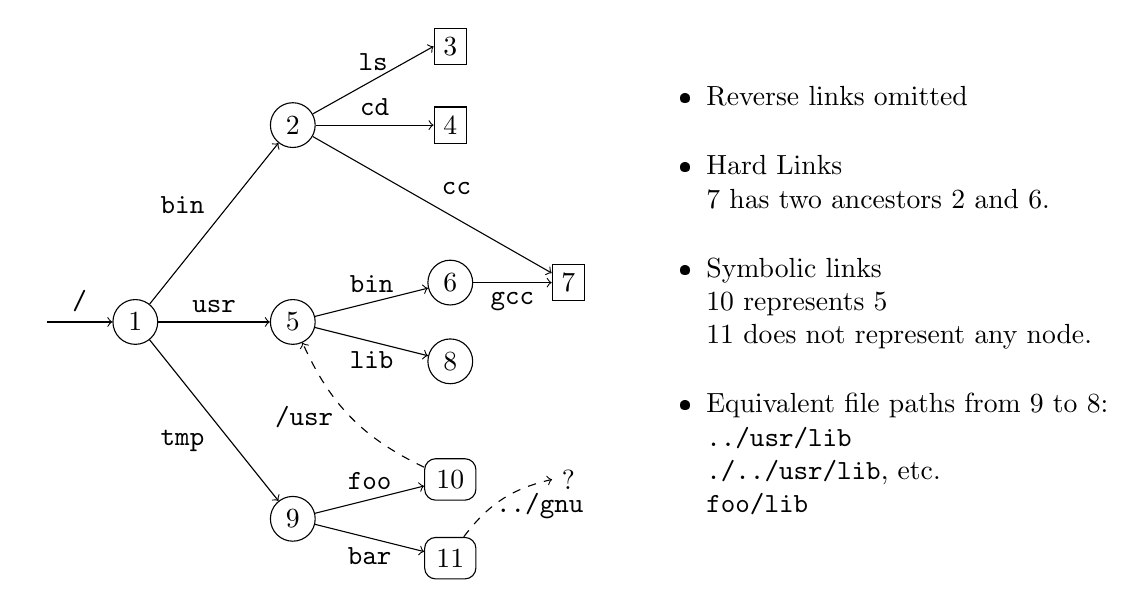
\begin{tikzpicture}
[dir/.style={draw, circle, inner sep=1mm},
 slink/.style={draw,rectangle,inner sep=1.5mm, rounded corners},
 file/.style={draw,rectangle},
 tpath/.style={font={\ttfamily},midway}]
\node (start) at (-1.25,0) {};
\node (n1) at (0,0) [dir] {1};

\node (n2) at (2,2.5) [dir] {2};
\node (n5) at (2,0) [dir] {5};
\node (n9) at (2,-2.5) [dir] {9};

\node (n3) at (4,3.5) [file] {3};
\node (n4) at (4,2.5) [file] {4};
\node (n6) at (4,0.5) [dir] {6};
\node (n8) at (4,-0.5) [dir] {8};
\node (n10) at (4, -2) [slink] {10};
\node (n11) at (4, -3) [slink] {11};

\node (n7) at (5.5, 0.5) [file] {7};
\node (nqmark) at (5.5, -2) {?};

\draw[->] (start) to node [tpath,above] {/} (n1);

\draw[->] (n1) to node [tpath,above left] {bin} (n2);
\draw[->] (n1) to node [tpath,above] {usr} (n5);
\draw[->] (n1) to node [tpath,below left] {tmp} (n9);

\draw[->] (n2) to node [tpath,above] {ls} (n3.west);
\draw[->] (n2) to node [tpath,above] {cd} (n4);
\draw[->] (n2) to node [tpath,above right] {cc} (n7);

\draw[->] (n5) to node [tpath,above] {bin} (n6);
\draw[->] (n5) to node [tpath,below] {lib} (n8);

\draw[->] (n9) to node [tpath,above] {foo} (n10);
\draw[->] (n9) to node [tpath,below] {bar} (n11);

\draw[->] (n6) to node [tpath,below] {gcc} (n7);

\draw[->,dashed] (n10) to [bend left=20] node [tpath,left=1mm] {/usr} (n5);
\draw[->,dashed] (n11) to [bend left=20] node [tpath,below right=-2mm] {../gnu} (nqmark.west);
\node[right=0.75cm, text width=6cm] at (n7)
{
  \begin{itemize}
    \item Reverse links omitted \vspace{5pt}
    \item Hard Links \\ 
      7 has two ancestors 2 and 6.\vspace{5pt}
    \item Symbolic links \\ 
      10 represents 5 \\ 
      11 does not represent any node. \vspace{5pt}
    \item Equivalent file paths from  9 to 8: \\
      \texttt{../usr/lib} \\
      \texttt{./../usr/lib}, {\etc} \\
      \texttt{foo/lib}
  \end{itemize}
};
\end{tikzpicture}
\end{myimage}
\caption{An example of a file hierarchy}
\label{fig/hierarchy}
\end{myfigure}

In general, a recursive traversal of the hierarchy will terminate
if the following rules are respected:
%
\begin{itemize}
\item the directories \ml+.+ and \ml+..+ are ignored.
\item symbolic links are not followed. 
\end{itemize}
% 
But if symbolic links are followed we are traversing a graph and
we need to keep track of the nodes we already visited to avoid loops.

Each process has a current working directory. It is returned by the
function \indexlibvalue{Unix}{getcwd} and can be changed with
\indexlibvalue{Unix}{chdir}.  It is also possible to constrict the
view of the file hierarchy by calling 
\indexlibvalue{Unix}{chroot} \ml+p+. This makes the node \ml+p+, which 
should be a directory, the root of the restricted view of the
hierarchy. Absolute file paths are then
interpreted according to this new root \ml+p+ (and of course \ml+..+ at the
new root is \ml+p+ itself).

\section{File names, file descriptors}

There are two ways to access a file.  The first is by its \emph{file
  name} (or \emph{path name}) in the file system hierarchy.  Due to
hard links, a file can have many different names.  Names are values of
type \ml+string+. For example the system calls \syscall{unlink},
\syscall{link}, \syscall{symlink} and \syscall{rename} all operate at
the file name level.
%
\begin{listingcodefile}{tmpunix.mli}
val $\libvalue{Unix}{unlink}$ : string -> unit
val $\libvalue{Unix}{link}$ : string -> string -> unit
val $\libvalue{Unix}{symlink}$ : string -> string -> unit
val $\libvalue{Unix}{rename}$ : string -> string -> unit
\end{listingcodefile}
% 
Their effect is as follows:
\begin{itemize}
\item \ml+unlink f+ erases the file \ml+f+ like the Unix command
\ml+rm -f f+.
%
\item \ml+link f1 f2+ creates a hard link named \ml+f2+ to
the file \ml+f1+ like the command \ml+ln f1 f2+.
%
\item \ml+symlink f1 f2+ creates a symbolic link named \ml+f2+ to the file 
\ml+f1+ like the command \ml+ln -s f1 f2+. 
%
\item \ml+rename f1 f2+ renames the file \ml+f1+ to \ml+f2+ 
like the command \ml+mv f1 f2+.
\end{itemize}

The second way of accessing a file is by a file descriptor. A
descriptor represents a pointer to a file along with other information
like the current read/write position in the file, the access rights of
the file (is it possible to read? write?) and flags which control the
behavior of reads and writes (blocking or non-blocking, overwrite,
append, \etc). File descriptors are values of the abstract type
\libtype{Unix}{file\_descr}.

Access to a file via its descriptor is independent from the
access via its name. In particular whenever we get a file descriptor,
the file can be destroyed or renamed but the descriptor still points
on the original file.

When a program is executed, three descriptors are allocated and 
tied to the variables \ml+stdin+, \ml+stdout+ and \ml+stderr+ of the
\ml+Unix+ module:
\begin{codefile}{tmpunix.mli}
type file_descr
\end{codefile}
\begin{listingcodefile}{tmpunix.mli}
val $\indexlibvalue{Unix}{stdin}$ : file_descr
val $\indexlibvalue{Unix}{stdout}$ : file_descr
val $\indexlibvalue{Unix}{stderr}$ : file_descr
\end{listingcodefile}
They correspond, respectively, to the standard input, standard output
and standard error of the process.

When a program is executed on the command line without any
redirections, the three descriptors refer to the terminal.  But if,
for example, the input has been redirected using the shell expression
\ml+cmd < f+, then the descriptor \ml+stdin+ refers to the file named \ml+f+
during the execution of the command \ml+cmd+. Similarly, \ml +cmd > f+
and \ml+cmd 2> f+ respectively bind the descriptors \ml+stdout+ and
\ml+stderr+ to the file named \ml+f+ during the execution of the
command.


\section{Meta-attributes, types and permissions}

The system calls \syscall{stat}, \syscall{lstat} and \syscall{fstat}
return the meta-attributes of a file. This is to say information about
the node itself rather than its content. Among other things, this
information contains the identity of the file, the type of file, the
access rights, the time and date of last access and other information.
%
\begin{codefile}{tmpunix.mli}
type stats
\end{codefile}
%
\begin{listingcodefile}{tmpunix.mli}
val $\libvalue{Unix}{stat}$  : string -> stats
val $\libvalue{Unix}{lstat}$ : string -> stats
val $\libvalue{Unix}{fstat}$ : file_descr -> stats
\end{listingcodefile}
% 
The system calls \ml+stat+ and \ml+lstat+ take a file name as an
argument while \ml+fstat+ takes a previously opened descriptor and
returns information about the file it points on.  \ml+stat+ and
\ml+lstat+ differ on symbolic links : \ml+lstat+ returns information
about the symbolic link itself, while \ml+stat+ returns information
about the file that the link points to. The result of these three
calls is a record of type \libtype{Unix}{stats} whose fields are
described in table~\ref{fig/stats}.
%
\begin{mytable}
\begin{tabular}{lp{9cm}}
Field name & Description \\
%
\hline
\ml+st_dev : int+ 
& The id of the device on which the file is stored. \\
%
\ml+st_ino : int+ 
& The id of the file (inode number) in its partition. 
The pair \ml+(st_dev, st_ino)+ uniquely identifies the file
within the file system. \\
%
\ml+st_kind : file_kind+ & 
The file type. The type \libtype{Unix}{file\_kind} is an enumerated type
whose constructors are:  
\begin{mltypecases}
\begin{tabular}{@{}ll}
\ml+S_REG+ & Regular file \\
\ml+S_DIR+ & Directory \\
\ml+S_CHR+ & Character device  \\
\ml+S_BLK+ & Block device  \\
\ml+S_LNK+ & Symbolic link \\
\ml+S_FIFO+ & Named pipe \\
\ml+S_SOCK+ & Socket 
\end{tabular}
\end{mltypecases}
\\
%
\ml+st_perm : int+ & Access rights for the file \\
%
\ml+st_nlink : int+ 
& For a directory: the number of entries in the directory. For others:
the number of hard links on this file. \\
%
\ml+st_uid : int+ & The id of the file's user owner. \\
%
\ml+st_gid : int+ & The id of the file's group owner. \\
%
\ml+st_rdev : int+ 
& The id of the associated peripheral (for special files). \\
%
\ml+st_size : int+ & The file size, in bytes. \\
%
\ml+st_atime : int+ & Last file content access date (in seconds from
January 1st 1970, midnight, \textsc{gmt}). \\
%
\ml+st_mtime : int+ & Last file content modification date (idem).\\
%
\ml+st_ctime : int+ & Last file state modification date: either a
write in the file or a change in access rights, user or group owner,
or number of links.
\smallskip\\
\hline
\end{tabular}
\caption{Fields of the \ml+stats+ structure}
\label{fig/stats}
\end{mytable}

\subsection*{Identification}

A file is uniquely identified by the pair made of its device number
(typically the disk partition where it is located) \ml+st_dev+ and its
inode number \ml+st_ino+.

\subsection*{Owners}

A file has one user owner \ml+st_uid+ and one group owner
\ml+st_gid+.  All the users and groups 
on the machine are usually described in the  
 \ml+/etc/passwd+ and \ml+/etc/groups+ files. We can look up them by
name in a portable manner with the functions \syscall{getpwnam} and 
\syscall{getgrnam} or by id with 
\syscall{getpwuid} and \syscall{getgrgid}.
%
\begin{codefile}{tmpunix.mli}
type passwd_entry = Unix.passwd_entry
type group_entry = Unix.group_entry
\end{codefile}
%
\begin{listingcodefile}{tmpunix.mli}
val $\libvalue{Unix}{getpwnam}$ : string -> passwd_entry
val $\libvalue{Unix}{getgrnam}$ : string -> group_entry
val $\libvalue{Unix}{getpwuid}$ : int -> passwd_entry
val $\libvalue{Unix}{getgrgid}$ : int -> group_entry
\end{listingcodefile}

The name of the user of a running process and all the groups
to which it belongs can be retrieved with the commands
\syscall{getlogin} and \syscall{getgroups}.
%
\begin{listingcodefile}{tmpunix.mli}
val $\libvalue{Unix}{getlogin}$ : unit -> string
val $\libvalue{Unix}{getgroups}$ : unit -> int array
\end{listingcodefile}

The call \syscall{chown} changes the owner (second argument) and the
group (third argument) of a file (first argument). If we have a file
descriptor, \syscall{fchown} can be used instead. Only the super user
can change this information arbitrarily.
%
\begin{listingcodefile}{tmpunix.mli}
val $\libvalue{Unix}{chown}$ : string -> int -> int -> unit
val $\libvalue{Unix}{fchown}$ : file_descr -> int -> int -> unit
\end{listingcodefile}

%% Le changement de groupe peut se faire sans privil�ge lorsque le
%% programme � un \ml+uid+ (effectif) �gal � celui du fichier et un
%% \ml+gid+ (effectif) �gal au group d�sir� ou � un de ses groupes
%% suppl�mentaire

\subsection*{Access rights}

Access rights are encoded as bits in an integer, the type 
\libtype{Unix}{file\_perm} is just an abbreviation for the type
\ml+int+. They specify special bits and read, write and
execution rights for the user owner, the group owner and the other
users as vector of bits:
%
\ifhtmlelse{%
\begin{center}
\begin{tabular}{ccc|ccc|ccc|ccc}
\multicolumn{3}{c}{\texttt{S}pecial}
&\multicolumn{3}{c}{\texttt{U}ser}
&\multicolumn{3}{c}{\texttt{G}roup}
&\multicolumn{3}{c}{\texttt{O}ther} \\
\hline
--&--&--&--&--&--&--&--&--&--&--&--\\
\hline
\multicolumn{12}{c}{\ml+OoSUGO+}
\end{tabular}
\end{center}
}
{%
\begin{displaymath}
\underbrace
{\overbrace{---}^{\texttt Special}
 \overbrace{---}^{\texttt User}
 \overbrace{---}^{\texttt Group}
 \overbrace{---}^{\texttt Other}}_{\texttt{0oSUGO}}
\end{displaymath}
}
% 
where in each of the user, group and other fields, the order of bits
indicates read (\ml+r+), write (\ml+w+) and execute (\ml+x+) rights.
The permissions on a file are the union of all these individual
rights, see table~\ref{tab/permbits}.

\begin{mytable}
\begin{tabular}{lcl}
Bit (octal) & Notation \ml+ls -l+ & Access right \\
\hline
\ml+0o100+ & \ml+--x------+ & executable by the user owner \\
\ml+0o200+ & \ml+-w-------+ & writable by the user owner \\
\ml+0o400+ & \ml+r--------+ & readable by the user owner \\
\hline
\ml+0o10+  & \ml+-----x---+ &
        executable by members of the group owner. \\
\ml+0o20+  & \ml+----w----+ &
        writable by members of the group owner. \\
\ml+0o40+  & \ml+---r----+ &
        readable by members of the group owner. \\
\hline
\ml+0o1+   & \ml+--------x+ & executable by other users\\
\ml+0o2+   & \ml+-------w-+ & writable by other users \\
\ml+0o4+   & \ml+------r--+ & readable by other users \\
\hline
\ml+0o1000+ & \ml+--------t+ & the bit \ml+t+ on the group (sticky bit)\\
\ml+0o2000+ & \ml+-----s---+ & the bit \ml+s+ on the group (\ml+set-gid+)\\
\ml+0o4000+ & \ml+--s------+ & the bit \ml+s+ on the user (\ml+set-uid+)\\
\hline
\end{tabular}
\caption{Permission bits}\label{tab/permbits}
\end{mytable}

For files, the meaning of read, write and execute permissions is
obvious. For a directory, the execute permission means the right to
enter it (to \ml+chdir+ to it) and read permission the right to list
its contents. Read permission on a directory is however not needed to
read its files or sub-directories (but we then need to know their
names).

The special bits do not have meaning unless the \ml+x+ bit is set (if
present without \ml+x+ set, they do not give additional rights).  This
is why their representation is superimposed on the bit \ml+x+ and
the letters \ml+S+ and \ml+T+ are used instead of \ml+s+ and \ml+t+
whenever \ml+x+ is not set. The bit \ml+t+ allows sub-directories to
inherit the permissions of the parent directory. On a directory, 
the bit \ml+s+ allows to use the directory's \ml+uid+ or \ml+gid+ rather
than the user's one to create directories. For an executable file, 
the bit \ml+s+ allows to change at execution time the user's
effective identity or group with the system calls \syscall{setuid} 
and \syscall{setgid}.
%
\begin{listingcodefile}{tmpunix.mli}
val $\libvalue{Unix}{setuid}$ : int -> unit
val $\libvalue{Unix}{setgid}$ : int -> unit
\end{listingcodefile}
%
The process also preserves its original identities unless 
it has super user privileges, in which case \ml+setuid+ and
\ml+setgid+ change both its effective and original user and group
identities. The original identity is preserved to allow 
the process to subsequently recover it as its effective identity
without needing further privileges. The system calls \syscall{getuid} and 
\syscall{getgid} return the original identities and 
\syscall{geteuid} and \syscall{getegid} return the effective identities.
%
\begin{listingcodefile}{tmpunix.mli}
val $\libvalue{Unix}{getuid}$ : unit -> int
val $\libvalue{Unix}{geteuid}$ : unit -> int
val $\libvalue{Unix}{getgid}$ : unit -> int
val $\libvalue{Unix}{getegid}$ : unit -> int
\end{listingcodefile}

A process also has a file creation mask encoded the same way file
permissions are. As its name suggests, the mask specifies prohibitions
(rights to mask): during file creation a bit set to 1 in the
mask is set to 0 in the permissions of the created file.  The mask
can be consulted and changed with the system call \syscall{umask}:
%
\begin{listingcodefile}{tmpunix.mli}
val $\libvalue{Unix}{umask}$ : int -> int
\end{listingcodefile}
% 
Like many system calls that modify system variables, the modifying
function returns the old value of the variable. Thus, to just look up
the value we need to call the function twice. Once with an arbitrary
value to get the mask and a second time to put it back. For example:
%
\begin{codefile}{tmpfich.ml}
open Unix;;
let _ = 
\end{codefile}
%
\begin{listingcodefile}{tmpfich.ml}
let m = umask 0 in ignore (umask m); m
\end{listingcodefile}

File access permissions can be modified with the system calls
\syscall{chmod} and \syscall{fchmod}:
%
\begin{codefile}{tmpunix.mli}
type file_perm
\end{codefile}
%
\begin{listingcodefile}{tmpunix.mli}
val $\libvalue{Unix}{chmod}$ : string -> file_perm -> unit
val $\libvalue{Unix}{fchmod}$ : file_descr -> file_perm -> unit
\end{listingcodefile}
and they can be tested \quotes{dynamically} with the system 
call \syscall{access}:
%
\begin{listingcodefile}{tmpunix.mli}
type $\libtype{Unix}{access\_permission}$ = R_OK | W_OK | X_OK | F_OK
val $\libvalue{Unix}{access}$ : string -> access_permission list -> unit 
\end{listingcodefile}
%
where requested access rights to the file are specified by a list of
values of type \libtype{Unix}{access\_permission} whose meaning is 
obvious except for \ml+F_OK+ which just checks for the file's
existence (without checking for the other rights). The function
raises an error if the access rights are not granted.

Note that the information inferred by \ml+access+ may be more
restrictive than the information returned by \ml+lstat+ because a file
system may be mounted with restricted rights~---~for example in
read-only mode. In that case \ml+access+ will deny a write permission
on a file whose meta-attributes would allow it. This is why we
distinguish between \quotes{dynamic} (what a process can actually do)
and \quotes{static} (what the file system specifies) information.

\section{Operations on directories}

Only the kernel can write in directories (when files are
created). Thus opening a directory in write mode is prohibited. In
certain versions of Unix a directory may be opened in read only mode
and read with \indexvalue{read}, but other versions prohibit
it. However, even if this is possible, it is preferable not to do so
because the format of directory entries vary between Unix versions and
is often complex. The following functions allow reading a directory
sequentially in a portable manner:
%
\begin{codefile}{tmpunix.mli}
type dir_handle = Unix.dir_handle
\end{codefile}
%
\begin{listingcodefile}{tmpunix.mli}
val $\libvalue{Unix}{opendir}$   : string -> dir_handle
val $\libvalue{Unix}{readdir}$   : dir_handle -> string
val $\libvalue{Unix}{rewinddir}$ : dir_handle -> unit
val $\libvalue{Unix}{closedir}$  : dir_handle -> unit
\end{listingcodefile}
% 
The system call \syscall{opendir} returns a directory descriptor on a
directory. \syscall{readdir} reads the next entry of a descriptor, it
returns a file name relative to the directory or raises the exception
\ml+End_of_file+ if the end of the directory is
reached. \syscall{rewinddir} repositions the descriptor at the
beginning of the directory and \syscall{closedir} closes the directory
descriptor.

\begin{example}
The following reusable function iterates a function \ml+f+ over the
entries of the directory \ml+dirname+.
%
\begin{codefile}{misc.mli}
(*** Directory iterator *)
val iter_dir : (string -> 'a) -> string -> unit
(** [iter_dir f d] opens path [d] as a directory and iterates the 
function [f] over all its entries *)
\end{codefile}
%
\begin{codefile}{misc.ml}
open Sys;;
open Unix;;
\end{codefile}
%
\begin{listingcodefile}{misc.ml}
let iter_dir f dirname =
  let d = opendir dirname in
  try while true do f (readdir d) done
  with End_of_file -> closedir d
\end{listingcodefile}
\end{example}

To create a directory or remove an empty directory, we have
\syscall{mkdir} and \syscall{rmdir}:
%
\begin{listingcodefile}{tmpunix.mli}
val $\libvalue{Unix}{mkdir}$ : string -> file_perm -> unit
val $\libvalue{Unix}{rmdir}$ : string -> unit
\end{listingcodefile}
% 
The second argument of \ml+mkdir+ determines the access rights of the
new directory.  Note that we can only remove a directory that is
already empty. To remove a directory and its contents, it is thus
necessary to first recursively empty the contents of the directory and
then remove the directory.

\section{\label{ex/find}Complete example: search in a file hierarchy}

The Unix command \ml+find+ lists the files of a hierarchy matching
certain criteria (file name, type and permissions \etc). In this
section we develop a library function \ml+Findlib.find+ which allows
to make these searches and a command \ml+find+ that provides a version
of the Unix command \ml+find+ restricted to the options \ml+-follow+
and \ml+-maxdepth+.

We specify the following interface for \ml+Findlib.find+:
%
\begin{listingcodefile}{findlib.mli}
val find : 
  (Unix.error * string * string -> unit) -> 
  (string -> Unix.stats -> bool) -> bool -> int -> string list -> 
  unit
\end{listingcodefile}
%
The function call
\begin{lstlisting}
find handler action follow depth roots
\end{lstlisting}
traverses the file hierarchy starting from the roots specified in the
list \ml+roots+ (absolute or relative to the current directory of the
process when the call is made) up to a maximum depth \ml+depth+ and following
symbolic links if the flag \ml+follow+ is set.  The paths found under
the root \ml+r+ include \ml+r+ as a prefix.  Each found path \ml+p+ is
given to the function \ml+action+ along with the data returned by
\ml+Unix.lstat p+ (or \ml+Unix.stat p+ if \ml+follow+ is \ml+true+).
The function \ml+action+ returns a boolean indicating, for
directories, whether the search should continue for its contents (\ml+true+)
or not (\ml+false+).

The \ml+handler+ function reports traversal errors of type
\ml+Unix_error+. Whenever an error occurs the arguments of the
exception are given to the handler function and the traversal
continues. However when an exception is raised by the functions
\ml+action+ or \ml+handler+ themselves, we immediately stop the
traversal and let it propagate to the caller. To propagate an
\ml+Unix_error+ exception without catching it like a traversal error,
we wrap these exceptions in the \ml+Hidden+ exception (see
\ml+hide_exn+ and \ml+reveal_exn+).
%
%%% commented in the french version
%% De plus on arr�te la visite r�cursive d'un r�pertoire que l'on est en train
%% de visiter (ce qui ne peut arriver que lorsqu'on suit les liens symboliques)
\begin{listingcodefile}[style=numbers]{findlib.ml}
open Unix;;

exception Hidden of exn
let hide_exn f x = try f x with exn -> raise (Hidden exn);;
let reveal_exn f x = try f x with Hidden exn -> raise exn;;

let find on_error on_path follow depth roots =
  let rec find_rec depth visiting filename =
    try
      let infos = (if follow then stat else lstat) filename in
      let continue = hide_exn (on_path filename) infos in
      let id = infos.st_dev, infos.st_ino in $\label{prog:did}$
      if infos.st_kind = S_DIR && depth > 0 && continue &&
        (not follow || not (List.mem id visiting))
      then
        let process_child child = 
          if (child <> Filename.current_dir_name &&
              child <> Filename.parent_dir_name) then 
            let child_name = Filename.concat filename child in
            let visiting = 
              if follow then id :: visiting else visiting in $\label{prog:follow}$
            find_rec (depth-1) visiting child_name in
        Misc.iter_dir process_child filename 
    with Unix_error (e, b, c) -> hide_exn on_error (e, b, c) in
  reveal_exn (List.iter (find_rec depth [])) roots;;
\end{listingcodefile}

A directory is identified by the \ml+id+ pair (line~\ref{prog:did})
made of its device and inode number.  The list \ml+visiting+ keeps
track of the directories that have already been visited. In fact
this information is only needed if symbolic links are followed
(line~\ref{prog:follow}).

It is now easy to program the \ml+find+ command. The essential part of
the code parses the command line arguments with the \libmodule{Arg}
module.
\begin{listingcodefile}{find.ml}
let find () =
  let follow = ref false in
  let maxdepth = ref max_int in
  let roots = ref [] in
  let usage_string  =
    ("Usage: " ^ Sys.argv.(0) ^ " [files...] [options...]") in
  let opt_list =  [ 
    "-maxdepth", Arg.Int ((:=) maxdepth), "max depth search";
    "-follow", Arg.Set follow, "follow symbolic links";
  ] in
  Arg.parse opt_list (fun f -> roots := f :: !roots) usage_string;
  let action p infos = print_endline p; true in
  let errors = ref false in
  let on_error (e, b, c) =
    errors := true; prerr_endline (c ^ ": " ^ Unix.error_message e) in
  Findlib.find on_error action !follow !maxdepth 
    (if !roots = [] then [ Filename.current_dir_name ] 
     else List.rev !roots);
  if !errors then exit 1;; 

Unix.handle_unix_error find ();;
\end{listingcodefile}
%
\begin{codefile}{find.test}
cd ../../lib/arch
./find.byte -follow -maxdepth 10 A B > find.out
find A B -follow -maxdepth 10 | diff - find.out
rm find.out
\end{codefile}
Although our \ml+find+ command is quite limited, the library
function \ml+FindLib.find+ is far more general, as the following
exercise shows.
\begin{exercise}
Use the function \ml+FindLib.find+ to write a command
\ml+find_but_CVS+ equivalent to the Unix command:
\begin{lstlisting}
find . -type d -name CVS -prune -o -print
\end{lstlisting}
which, starting from the current directory, recursively prints
files without printing or entering directories whose name is \ml+CVS+.
\end{exercise}
\begin{answer}
\begin{codefile}{find_but_CVS.ml}
open Unix;;
open Misc;;
\end{codefile}
%
\begin{listingcodefile}{find_but_CVS.ml}
let main () = 
  let action p infos = 
    let b = not (infos.st_kind = S_DIR || Filename.basename p = "CVS") in
    if b then print_endline p; b in
  let errors = ref false in
  let error (e,c,b) = 
    errors:= true; prerr_endline (b ^ ": " ^ error_message e) in
  Findlib.find error action false max_int [ "." ];;
handle_unix_error main ()
\end{listingcodefile}
\end{answer}

\begin{exercise}
The function \ml+getcwd+ is not a system call but is defined in the
\ml+Unix+ module.  Give a \quotes{primitive} implementation of
\ml+getcwd+. First describe the principle of your algorithm with words
and then implement it (you should avoid repeating the same system
call).
\end{exercise}
\begin{answer}
Here are some hints. We move up from the current position towards the
root and construct backwards the path we are looking for. The root can
be detected as the only directory node whose parent is equal to itself
(relative to the root \ml+.+ and \ml+..+ are equal). To find the name
of a directory \ml+r+ we need to list the contents of its parent
directory and detect the file that corresponds to \ml+r+.
\end{answer}

\section{Opening a file}

The \ml+openfile+ function allows us to obtain a descriptor on
a file of a given name (the corresponding system call
is \syscall{open}, however \ml+open+ is a keyword in {\ocaml}).
%
\begin{codefile}{tmpunix.mli}
type open_flag = Unix.open_flag;;
\end{codefile}
%
\begin{listingcodefile}{tmpunix.mli}
val $\libvalue{Unix}{openfile}$ : 
 string -> open_flag list -> file_perm -> file_descr
\end{listingcodefile}
% 
The first argument is the name of the file to open. The second
argument, a list of flags from the enumerated type
\libtype{Unix}{open\_flag}, describes the mode in which the file should
be opened and what to do if it does not exist. The third argument of
type \libtype{Unix}{file\_perm} defines the file's access rights,
should the file be created.  The result is a file descriptor on the
given file name with the read/write position at the beginning of the
file.

The flag list must contain exactly one of the following flags:
%
\begin{mltypecases}
\begin{tabular}{@{}ll}
\ml+O_RDONLY+ & Open in read-only mode. \\
\ml+O_WRONLY+ & Open in write-only mode. \\
\ml+O_RDWR+ & Open in read and write mode.
\end{tabular}
\end{mltypecases}
% 
These flags determine whether read or write calls can be done on the
descriptor. The call \ml+openfile+ fails if a process asks to open a
file in write (resp. read) mode on a file on which it has no right to
write (resp. read). For this reason \ml+O_RDWR+ should not be used
systematically.

The flag list can also contain one or more of the following values:
%
\begin{mltypecases}
\begin{tabular}{@{}ll}
\ml+O_APPEND+ & Open in append mode. \\
\ml+O_CREAT+ & Create the file if it does not exist. \\
\ml+O_TRUNC+ & Truncate the file to zero if it already exists. \\
\ml+O_EXCL+ & Fail if the file already exists.
\end{tabular}
\end{mltypecases}
\begin{mltypecases}
\begin{tabular}{@{}ll}
\ml+O_NONBLOCK+ &  Open in non-blocking mode. \\
\ml+O_NOCTTY+ & Do not function in console mode.
\end{tabular}
\end{mltypecases}
\begin{mltypecases}
\begin{tabular}{@{}ll}
\ml+O_SYNC+  & Perform the writes in synchronous mode. \\
\ml+O_DSYNC+ & Perform the data writes in synchronous mode. \\
\ml+O_RSYN+ & Perform the reads in synchronous mode. 
\end{tabular}
\end{mltypecases}
%
The first group defines the behavior to follow if
the file exists or not. With:
\begin{itemize}
\item \ml+O_APPEND+, the read/write position will be set at the end of
  the file before each write. Consequently any written data will be
  added at the end of file. Without \ml+O_APPEND+, writes occur at the
  current read/write position (initially, the beginning of the file).

\item \ml+O_TRUNC+, the file is truncated when it
is opened. The length of the file is set to zero and the bytes
contained in the file are lost, writes start from an empty file. 
Without \ml+O_TRUNC+, the writes are made at the start of the file
overwriting any data that may already be there.

\item \ml+O_CREAT+, creates the file if it does not exist. The created
  file is empty and its access rights are specified by the third argument 
  and the creation mask of the process (the mask can be retrieved 
  and changed with \libvalue{Unix}{umask}).

\item \ml+O_EXCL+, \ml+openfile+ fails if the file already exists.
  This flag, used in conjunction with \ml+O_CREAT+ allows to use
  files as \label{page/lock}\emph{locks}\footnote{This is not 
    possible if the lock file
    is located on a \textsc{nfs} partition, because \textsc{nfs} does
    not implement the option \ml+O_CREAT+ of \ml+open+ correctly.}. A process
  which wants to take the lock calls \ml+openfile+ on the file with
  \ml+O_EXCL+ and \ml+O_CREAT+. If the file already exists, this means
  that another process already holds the lock and \ml+openfile+ raises
  an error. If the file does not exist \ml+openfile+ returns without
  error and the file is created, preventing other processes from
  taking the lock. To release the lock the process calls
  \ml+unlink+ on it. The creation of a file is an atomic operation: if
  two processes try to create the same file in parallel with the
  options \ml+O_EXCL+ and \ml+O_CREAT+, at most one of them can
  succeed. The drawbacks of this technique is that a process must
  busy wait to acquire a lock that is currently hold and
  the abnormal termination of a process holding a lock may never
  release it.
\end{itemize}

\begin{example} 
Most programs use \ml+0o666+ for the third argument
to \ml+openfile+. This means \ml+rw-rw-rw-+ in symbolic notation. 
With the default creation mask of \ml+0o022+, the
file is thus created with the permissions \ml+rw-r--r--+. With a more 
lenient mask of \ml+0o002+, the file is created with the permissions 
\ml+rw-rw-r--+.
\end{example}

\begin{example} 
To read from a file:
%
\begin{lstlisting}
openfile filename [O_RDONLY] 0
\end{lstlisting}
%
The third argument can be anything as \ml+O_CREAT+ is not specified, 0
is usually given.

To write to an empty a file without caring about any previous content:
%
\begin{lstlisting}
openfile filename [O_WRONLY; O_TRUNC; O_CREAT] 0o666
\end{lstlisting}
%
If the file will contain executable code (\eg{} files
created by \ml+ld+, scripts, \etc), we create it with execution permissions:
%
\begin{lstlisting}
openfile filename [O_WRONLY; O_TRUNC; O_CREAT] 0o777
\end{lstlisting}
%
If the file must be confidential (\eg{} \quotes{mailbox} files where
\ml+mail+ stores read messages), we create it with write permissions
only for the user owner:
%
\begin{lstlisting}
openfile filename [O_WRONLY; O_TRUNC; O_CREAT] 0o600
\end{lstlisting}
%
To append data at the end of an existing file or create it if it 
doesn't exist:
%
\begin{lstlisting}
openfile filename [O_WRONLY; O_APPEND; O_CREAT] 0o666
\end{lstlisting}
\end{example}

The \ml+O_NONBLOCK+ flag guarantees that if the file is a named pipe
or a special file then the file opening and subsequent reads and
writes will be non-blocking.

The \ml+O_NOCTYY+ flag guarantees that if the file is a control
terminal (keyboard, window, \etc), it won't become the controlling
terminal of the calling process. 

The last group of flags specifies how to synchronize 
read and write operations. By default these operations are not
synchronized. With:
\begin{itemize}
\item\ml+O_DSYNC+, the data is written synchronously such that
  the process is blocked until all the writes have been done
  physically on the media (usually a disk). 
%
\item\ml+O_SYNC+, the file data and its meta-attributes are written 
  synchronously.
%
\item\ml+O_RSYNC+, with \ml+O_DSYNC+ specifies that the data reads are
  also synchronized: it is guaranteed that all current writes
  (requested but not necessarily performed) to the file are really
  written to the media before the next read.  If \ml+O_RSYNC+ is
  provided with \ml+O_SYNC+ the above also applies to meta-attributes
  changes.
\end{itemize}


\section{Reading and writing}

The system calls \syscall{read} and \syscall{write} read and write
bytes in a file. For historical reasons, the system
call \ml+write+ is provided in {\ocaml} under the name
\ml+single_write+:
%
\begin{listingcodefile}{tmpunix.mli}
val $\libvalue{Unix}{read}$  : file_descr -> string -> int -> int -> int
val $\libvalue{Unix}{single\_write}$ : file_descr -> string -> int -> int -> int
\end{listingcodefile}
% 
The two calls \ml+read+ and \ml+single_write+ have the same
interface. The first argument is the file descriptor to act on.  The
second argument is a string which will hold the read bytes (for
\ml+read+) or the bytes to write (for \ml+single_write+). The third
argument is the position in the string of the first byte to be written
or read. The fourth argument is the number of the bytes to be read or
written. In fact the third and fourth argument define a sub-string of
the second argument (the sub-string should be valid, \ml+read+ and
\ml+single_write+ do not check this).
%
\begin{myimage}[width="85\%"]
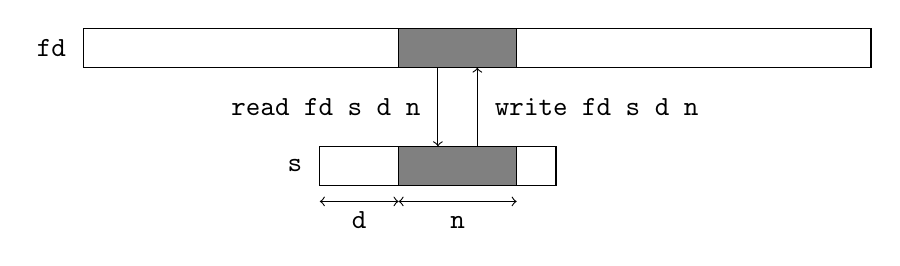
\begin{tikzpicture}[font={\ttfamily}]
\path[draw,fill=gray] (1,1.5) rectangle +(1.5, 0.5);
\path[draw] (-3,1.5) rectangle +(10, 0.5);
\node[anchor=east] at (-3.1,1.75) {fd};

\draw[->] (1.5, 1.5) to node [left=1mm] {read fd s d n} (1.5, 0.5);
\draw[<-] (2, 1.5) to node [right=1mm] {write fd s d n} (2, 0.5);

\path[draw,fill=gray] (1,0) rectangle +(1.5, 0.5);
\path[draw] (0,0) rectangle (3, 0.5);
\node[anchor=east] at (-0.1,0.25) {s};

\draw[<->] (0,-0.2) to node [below] {\phantom{n}d\phantom{n}} (1,-0.2);
\draw[<->] (1,-0.2) to node [below] {\phantom{d}n\phantom{d}} (2.5,-0.2);
\end{tikzpicture}
\end{myimage}
%
\ml+read+ and \ml+single_write+ return the number of bytes actually
read or written.

Reads and write calls are performed from the file descriptor's current
read/write position (if the file was opened in \ml+O_APPEND+ mode,
this position is set at the end of the file prior to any
write). After the system call, the current position is advanced by
the number of bytes read or written.

For writes, the number of bytes actually written is usually the number
of bytes requested. However there are exceptions: (i) if it is not
possible to write the bytes (\eg{} if the disk is full) (ii) the
descriptor is a pipe or a socket open in non-blocking mode (iii) due to
{\ocaml}, if the write is too large.

The reason for (iii) is that internally {\ocaml} uses auxiliary
buffers whose size is bounded by a maximal value. If this value is
exceeded the write will be partial. To work around this problem
{\ocaml} also provides the function \libvalue{Unix}{write} which
iterates the writes until all the data is written or an error occurs.
The problem is that in case of error there's no way to know the number
of bytes that were actually written. Hence \ml+single_write+ should be
preferred because it preserves the atomicity of writes (we know
exactly what was written) and it is more faithful to the original Unix
system call (note that the implementation of \ml+single_write+ is
described in section~\ref{single_write}).

%%% The french version has that here, but I don't think it belongs
%%% here.
%% In the following chapter, we shall see that when we write to a 
%% file descriptor which refers to a pipe or a lock file placed
%% in input/output blocking mode and which is then interrupted by a signal,
%% the call \ml+single_write+ returns an error \ml+EINTR+.
  
\begin{example} 
Assume \ml+fd+ is a descriptor open in write-only mode. 
%
\begin{lstlisting}
write fd "Hello world!" 3 7
\end{lstlisting}
%
writes the characters \ml+"lo worl"+ in the corresponding file,
and returns 7.
\end{example}

For reads, it is possible that the number bytes actually read is
smaller than the number of requested bytes. For example when the end
of file is near, that is when the number of bytes between the current
position and the end of file is less than the number of requested
bytes. In particular, when the current position is at the end of file,
\ml+read+ returns zero. The convention \quotes{zero equals end of
  file} also holds for special files, pipes and sockets. For example,
\ml+read+ on a terminal returns zero if we issue a \ml+ctrl-D+ on the
input.

Another example is when we read from a terminal. In that case,
\ml+read+ blocks until an entire line is available. If the line length
is smaller than the requested bytes \ml+read+ returns immediately with
the line without waiting for more data to reach the number of
requested bytes. (This is the default behavior for terminals, but it
can be changed to read character-by-character instead of
line-by-line, see section~\ref{sec/speciaux} and the type
\libtype{Unix}{terminal\_io} for more details.)

\begin{example} 
The following expression reads at most 100 characters from standard
input and returns them as a string.
%
\begin{lstlisting}
let buffer = String.create 100 in
let n = read stdin buffer 0 100 in
  String.sub buffer 0 n
\end{lstlisting}
\end{example}

\begin{example} 
The function \ml+really_read+ below has the same interface as
\ml+read+, but makes additional read attempts to try to get
the number of requested bytes. It raises the exception
\ml+End_of_file+ if the end of file is reached while doing this.
%
\begin{lstlisting}
let rec really_read fd buffer start length =
  if length <= 0 then () else
  match read fd buffer start length with
  | 0 -> raise End_of_file
  | r -> really_read fd buffer (start + r) (length - r);;
\end{lstlisting}
%
\end{example}

\section{Closing a descriptor}

The system call \syscall{close} closes a file descriptor.
%
\begin{listingcodefile}{tmpunix.mli}
val $\libvalue{Unix}{close}$ : file_descr -> unit
\end{listingcodefile}
% 

Once a descriptor is closed, all attempts to read, write, or do
anything else with the descriptor will fail. Descriptors should be
closed when they are no longer needed; but it is not mandatory. In
particular, and in contrasts to what happen with \ml+Pervasives+'
channels, a file descriptor doesn't need to be closed to ensure that
all pending writes have been performed as write requests made with
\ml+write+ are immediately transmitted to the kernel. On the other
hand, the number of descriptors allocated by a process is limited by
the kernel (from several hundreds to thousands). Doing a \ml+close+ on
an unused descriptor releases it, so that the process does not run out
of descriptors.

\section{\label{ex/filecopy}Complete example: file copy}

We program a command \ml+file_copy+ which, given two arguments 
\ml+f1+ and \ml+f2+, copies in the file \ml+f2+ the bytes contained 
in \ml+f1+.
%
\begin{listingcodefile}{file_copy.ml}
open Unix;;

let buffer_size = 8192;;
let buffer = String.create buffer_size;;

let file_copy input_name output_name =
  let fd_in = openfile input_name [O_RDONLY] 0 in
  let fd_out = openfile output_name [O_WRONLY; O_CREAT; O_TRUNC] 0o666 in
  let rec copy_loop () = match read fd_in buffer 0 buffer_size with
    |  0 -> ()
    | r -> ignore (write fd_out buffer 0 r); copy_loop () 
  in
  copy_loop ();
  close fd_in;
  close fd_out;;
\end{listingcodefile}
%
\begin{codefile}{copy.ml}
open Unix
open File_copy
\end{codefile}
%
\begin{listingcodefile}{copy.ml}
let copy () =
  if Array.length Sys.argv = 3 then begin
    file_copy Sys.argv.(1) Sys.argv.(2);
    exit 0
  end else begin
    prerr_endline 
      ("Usage: " ^ Sys.argv.(0) ^ " <input_file> <output_file>");
    exit 1
  end;;

handle_unix_error copy ();;
\end{listingcodefile}
%

The bulk of the work is performed by the the function \ml+file_copy+.
First we open a descriptor in read-only mode on the input file and
another in write-only mode on the output file. 

If the output file already exists, it is truncated (option
\ml+O_TRUNC+) and if it does not exist it is created (option
\ml+O_CREAT+) with the permissions \ml+rw-rw-rw-+ modified by the creation
mask. (This is unsatisfactory: if we copy an executable file, we would
like the copy to be also executable. We will see later how to give
a copy the same permissions as the original.)

In the \ml+copy_loop+ function we do the copy by blocks of
\ml+buffer_size+ bytes. We request \ml+buffer_size+ bytes to read. If
\ml+read+ returns zero, we have reached the end of file and the copy
is over. Otherwise we write the \ml+r+ bytes we have read in the
output file and start again.

Finally, we close the two descriptors. The main program \ml+copy+
verifies that the command received two arguments and passes them to
the function \ml+file_copy+.

Any error occurring during the copy results in a \ml+Unix_error+
catched and displayed by \ml+handle_unix_error+. Example of errors
include inability to open the input file because it does not
exist, failure to read because of restricted permissions, failure to
write because the disk is full, \etc

\begin{exercise} 
Add an option \ml+-a+ to the program, such that 
\ml+file_copy -a f1 f2+ appends the contents of \ml+f1+ to the end of
the file \ml+f2+. 
\end{exercise}
\begin{answer}
If the option \ml+-a+ is supplied, we need to do 
%
\begin{lstlisting}
openfile output_name [O_WRONLY; O_CREAT; O_APPEND] 0o666
\end{lstlisting}
%
instead of
%
\begin{lstlisting}
openfile output_name [O_WRONLY; O_CREAT; O_TRUNC] 0o666
\end{lstlisting}
%
Parsing the new option from the command line is left to the reader. 
\end{answer}

\section{The cost of system calls. The buffers.}

In the example \ml+file_copy+, reads were made in blocks of 8192
bytes. Why not read byte per by byte, or megabyte per by megabyte?
For efficiency reasons. 

Figure~\ref{fig/copy-speed} shows the copy speed of \ml+file_copy+, in
bytes per second, against the size of blocks (the value
\ml+buffer_size+). The amount of data transferred is the same
regardless of the size of the blocks.
\begin{myfigure}
\begin{myimage}[width="100\%"]
\begin{tikzpicture}[font=\tiny]
\pgfsetplotmarksize{0.8pt}
\draw plot[only marks,mark=*] file {data/speed-log.data};

% x-axis
\draw (0,-1) -- (7,-1);
\foreach \x in {0,...,7} { \draw (\x,-1) -- (\x,-0.95); };
\node at (0,-1.3) {\phantom{$^{2}$}1\phantom{$^{2}$}};
\node at (1,-1.3) {\phantom{$^{2}$}10\phantom{$^{2}$}};
\node at (2,-1.3) {\phantom{$^{2}$}100\phantom{$^{2}$}};
\foreach \x in {3,...,7} { \node at (\x,-1.3) {\phantom{$^{\x}$}10$^\x$}; };
\node at (8.5, -1.3) {Size (bytes)\phantom{1$^{1}$}};

% y-axis
\draw (-0.5,-0.5) -- (-0.5, 2.5);
\foreach \y in {-1,...,3} { \draw (-0.5,\y) -- (-0.45,\y); };
\node[anchor=east] at (-0.5,-1) {0.1\phantom{$^{3}$}};
\node[anchor=east] at (-0.5,0) {1\phantom{$^{3}$}};
\node[anchor=east] at (-0.5,1) {10\phantom{$^{3}$}};
\node[anchor=east] at (-0.5,2) {100\phantom{$^{3}$}};
\node[anchor=east] at (-0.5,3) {10$^{3}$};

\node[anchor=east] at (-0.5,3.5) {Speed (MB/s)};
\end{tikzpicture}
\end{myimage}
\caption{Copy speed as a function of block size}
\label{fig/copy-speed}
\end{myfigure}
For small block sizes, the copy speed is almost proportional to the
block size. Most of the time is not spent in data transfers but in the
execution of the loop \ml+copy_loop+ and in the calls to \ml+read+ and
\ml+write+. By profiling more carefully we can see that most of the
time is spent in the calls to \ml+read+ and \ml+write+. We conclude
that a system call, even if it has not much to do, takes a minimum of
about 4 micro-seconds (on the machine that was used for the test~---~a
2.8 GHz Pentium 4 ), let us say from 1 to 10 microseconds.  For small
input/output blocks, the duration of the system call dominates.
  
For larger blocks, between 4KB and 1MB, the copy speed is constant and
maximal. Here, the time spent in system calls and the loop is small
relative to the time spent on the data transfer. Also the buffer
size becomes bigger than the cache sizes used by the system and the
time spent by the system to make the transfer dominates the cost of a
system call\footnote{In fact, {\ocaml} limits the size of data
  transfers to 16KB (in the current version) and repeats \ml+write+
  system calls to make the complete transfer~---~see the discussion in
  section~\ref{single_write}. But this limit is bigger than the
  size of system caches and it not observable.}

Finally, for very large blocks (8MB and more) the speed is slightly
under the maximum.  Coming into play here is the time needed to
allocate the block and assign memory pages to it as it fills up.

\begin{codefile}{speed_write.c}
#include <errno.h>
#include <string.h>
#include <caml/mlvalues.h>
#include <caml/memory.h>
#include <caml/signals.h>
#include <caml/unixsupport.h>

#define LONG_BUFFER_SIZE 9388608

CAMLprim value speed_write
        (value fd, value buf, value ofs, value len) {
  CAMLparam4(fd, buf, ofs, len);
  long numbytes;
  int ret = 0;
  char iobuf[LONG_BUFFER_SIZE];
  numbytes = Long_val(len);
  if (numbytes > LONG_BUFFER_SIZE) numbytes = LONG_BUFFER_SIZE;
  /* memmove (iobuf, &Byte(buf, Long_val(ofs)), numbytes); */
  /* enter_blocking_section (); */
  /* ret = write(Int_val(fd), iobuf, (int) numbytes); */
  ret = write(Int_val(fd), &Byte(buf, Long_val(ofs)), (int) numbytes);
  /* leave_blocking_section (); */
  if (ret == -1) uerror("write", Nothing);
  CAMLreturn (Val_int(ret));
}
\end{codefile}
%
\begin{codefile}{speed.ed}
f speed.ml
r file_copy.ml
3a
external speed_write :
   file_descr -> string -> int -> int -> int = "speed_write";;
.
/buffer_size/,/file_copy/c
let file_copy buffer_size input_name output_name =
  let buffer = String.create buffer_size in
.
/write/s/write/speed_write/
$a

let rec power n k = if k > 0 then n * power n (pred k) else 1;;
let copy () =
  if Array.length Sys.argv = 2 then begin
    let file = Sys.argv.(1) in
    let tmp = Filename.temp_file "foo" "bar" in
    let mega_octets = float (10 * (lstat file).st_size) /. 1e6 in
    (* put file in cache *)
    file_copy 10 file "/dev/null";
    for i = 23 downto 0 do 
      let start = let t = Unix.times () in t.tms_utime +. t.tms_stime in
      let block = power 2 i in
      for i = 1 to 10 do file_copy block file tmp done;
      let stop = let t = Unix.times () in t.tms_utime +. t.tms_stime in
      let time = stop -. start in
      let speed = mega_octets /. time in
      Printf.printf "%9d %.2f" block speed; 
      print_newline ();
    done;
      exit 0
  end else begin
    prerr_endline ("Usage: " ^Sys.argv.(0)^ " <input_file> <output_file>");
    exit 1
  end;;

handle_unix_error copy ();;
.
wq
\end{codefile}
% $

Moral of the story, a system call, even if it does very little work,
costs dearly~---~much more than a normal function call: roughly, 2 to
20 microseconds for each system call, depending on the the
architecture. It is therefore important to minimize the number of
system calls. In particular, read and write operations should be made
in blocks of reasonable size and not character by character.

In examples like \ml+file_copy+, it is not difficult to do
input/output with large blocks. But other types of programs are more
naturally written with character by character input or output (\eg{}
reading a line from a file, lexical analysis, display a number \etc).
To satisfy the needs of these programs, most systems provide
input/output libraries with an additional layer of software between
the application and the operating system. For example, in {\ocaml} the
\ml+Pervasives+ module defines the abstract types
\libtype{Pervasives}{in\_channel} and
\libtype{Pervasives}{out\_channel}, similar to file descriptors, and
functions on these types like \libvalue{Pervasives}{input\_char},
\libvalue{Pervasives}{input\_line},
\libvalue{Pervasives}{output\_char}, or
\libvalue{Pervasives}{output\_string}.  This layer uses buffers to
group sequences of character by character reads or writes into a
single system call to read or write. This results in better
performance for programs that proceed character by character.
Moreover this additional layer makes programs more portable: we just
need to implement this layer with the system calls provided by another
operating system to port all the programs that use this library on
this new platform.

\section{Complete example: a small input/output library}

To illustrate the buffered input/output techniques, we implement a fragment
of {\ocaml} \ml+Pervasives+' channels. Here is the interface:
%
\begin{listingcodefile}{io.mli}
exception End_of_file

type in_channel
val open_in : string -> in_channel
val input_char : in_channel -> char
val close_in : in_channel -> unit

type out_channel
val open_out : string -> out_channel
val output_char : out_channel -> char -> unit
val close_out : out_channel -> unit
\end{listingcodefile}
%
We start with the \quotes{input} part. The abstract type 
\ml+in_channel+ is defined as follows: 
%
\begin{listingcodefile}{io.ml}
open Unix;;

type in_channel =
  { in_buffer: string;
    in_fd: file_descr;
    mutable in_pos: int;
    mutable in_end: int };;
exception End_of_file
\end{listingcodefile}
%
The character string of the \ml+in_buffer+ field is, literally, the
buffer.  The field \ml+in_fd+ is a (Unix) file descriptor, opened on
the file to read. The field \ml+in_pos+ is the current read position
in the buffer.  The field \ml+in_end+ is the number of valid
characters preloaded in the buffer.
%
\begin{myimage}[width="85\%"]
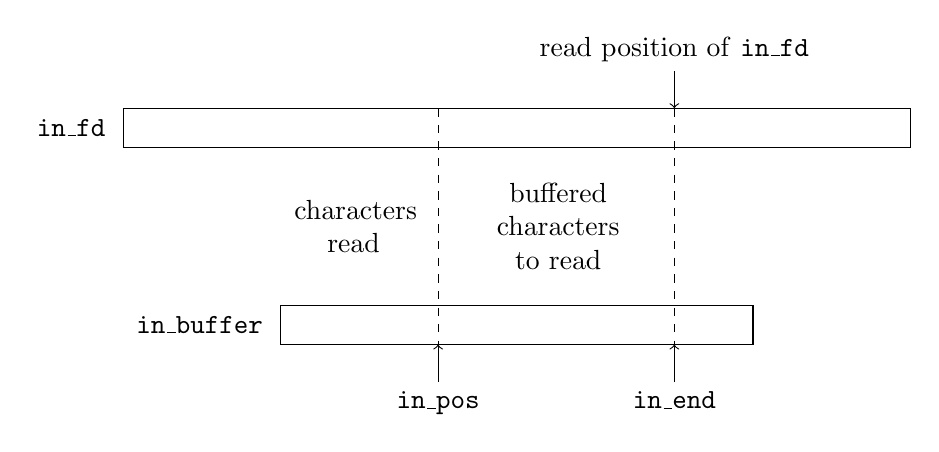
\begin{tikzpicture}
\path[draw] (-3,2.5) rectangle +(10, 0.5);
\node[anchor=east] at (-3.1,2.75) {\texttt{in\_fd}};
\draw[dashed] (1,3) to node [left=2mm,text width=1.5cm,text centered] 
 {characters read} (1,0);

\draw[dashed] (4,3) to node [left=1mm,text width=2.5cm,text centered] 
 {buffered characters to read} (4,0);

\path[draw] (-1,0) rectangle +(6, 0.5);
\node[anchor=east] at (-1.1,0.25) {\texttt{in\_buffer}};

\node (fdpos) at (4,3.75) {read position of \texttt{in\_fd}};
\draw[->] (fdpos.south) to (4,3);

\node (ipos) at (1,-0.75) {\texttt{\phantom{d}in\_pos\phantom{d}}};
\node (iend) at (4,-0.75) {\texttt{\phantom{p}in\_end\phantom{p}}};
\draw[->] (ipos.north) to (1,0);
\draw[->] (iend.north) to (4,0);
\end{tikzpicture}
\end{myimage}
The fields \ml+in_pos+ and \ml+in_end+ will be modified in place during 
read operations; we therefore declare them as \ml+mutable+.
%
\begin{listingcodefile}{io.ml}
let buffer_size = 8192;;
let open_in filename =
  { in_buffer = String.create buffer_size;
    in_fd = openfile filename [O_RDONLY] 0;
    in_pos = 0;
    in_end = 0 };;
\end{listingcodefile}
%
When we open a file for reading, we create a buffer of reasonable size
(large enough so as not to make too many system calls; small enough so
as not to waste memory). We then initialize the field \ml+in_fd+ with
a Unix file descriptor opened in read-only mode on the given file. The
buffer is initially empty (it does not contain any character from the
file); the field \ml+in_end+ is therefore initialized to zero.
%
\begin{listingcodefile}{io.ml}
let input_char chan =
  if chan.in_pos < chan.in_end then begin
    let c =  chan.in_buffer.[chan.in_pos] in
      chan.in_pos <- chan.in_pos + 1;
      c
  end else begin
    match read chan.in_fd chan.in_buffer 0 buffer_size
    with 0 -> raise End_of_file
       | r -> chan.in_end <- r;
              chan.in_pos <- 1;
              chan.in_buffer.[0]
  end;;
\end{listingcodefile}
% 
To read a character from an \ml+in_channel+, we do one of two
things.  Either there is at least one unread character in the buffer;
that is to say, the field \ml+in_pos+ is less than the field
\ml+in_end+. We then return this character located at \ml+in_pos+, and
increment \ml+in_pos+. Or the buffer is empty and we call \ml+read+ to
refill the buffer. If \ml+read+ returns zero, we have reached the end
of the file and we raise the exception \ml+End_of_file+. Otherwise, we
put the number of characters read in the field \ml+in_end+ (we may
receive less characters than we requested, thus the buffer may be
only partially refilled) and we return the first character read.
%
\begin{listingcodefile}{io.ml}
let close_in chan =
  close chan.in_fd;;
\end{listingcodefile}
%
Closing an \ml+in_channel+ just closes the underlying Unix file descriptor. 

The \quotes{output} part is very similar to the \quotes{input}
part. The only asymmetry is that the buffer now contains incomplete
writes (characters that have already been buffered but not written to
the file descriptor), and not reads in advance (characters that have
buffered, but not yet read).

\begin{myimage}[width="85\%"]
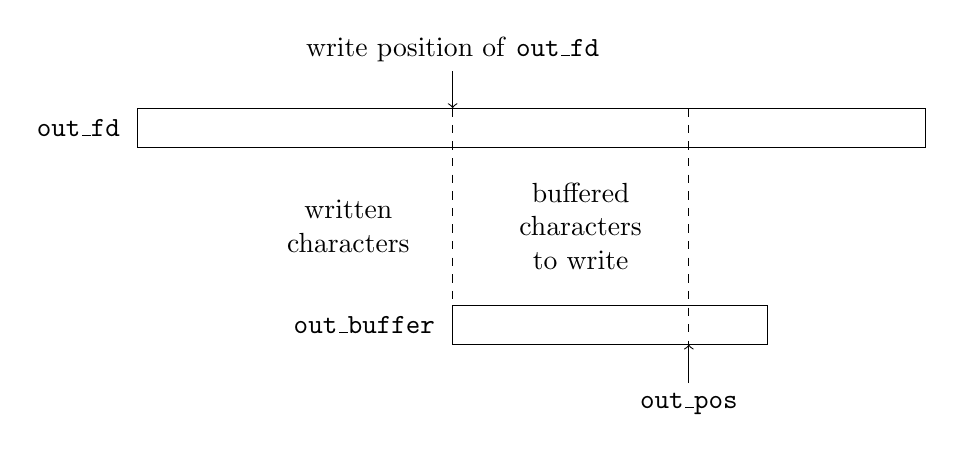
\begin{tikzpicture}
\path[draw] (-3,2.5) rectangle +(10, 0.5);
\node[anchor=east] at (-3.1,2.75) {\texttt{out\_fd}};
\draw[dashed] (1,3) to node [left=2mm,text width=2cm,text centered] 
 {written characters} (1,0);

\draw[dashed] (4,3) to node [left,text width=2.5cm,text centered] 
 {buffered characters to write} (4,0);

\path[draw] (1,0) rectangle +(4, 0.5);
\node[anchor=east] at (0.9,0.25) {\texttt{out\_buffer}};

\node (fdpos) at (1,3.75) {write position of \texttt{out\_fd}};
\draw[->] (fdpos.south) to (1,3);

\node (opos) at (4,-0.75) {\texttt{out\_pos}};
\draw[->] (opos.north) to (4,0);
\end{tikzpicture}
\end{myimage}
%
\begin{listingcodefile}{io.ml}
type out_channel =
  { out_buffer: string;
    out_fd: file_descr;
    mutable out_pos: int };;

let open_out filename =
  { out_buffer = String.create 8192;
    out_fd = openfile filename [O_WRONLY; O_TRUNC; O_CREAT] 0o666;
    out_pos = 0 };;

let output_char chan c =
  if chan.out_pos < String.length chan.out_buffer then begin
    chan.out_buffer.[chan.out_pos] <- c;
    chan.out_pos <- chan.out_pos + 1
  end else begin
    ignore (write chan.out_fd chan.out_buffer 0 chan.out_pos);
    chan.out_buffer.[0] <- c;
    chan.out_pos <- 1
  end;;

let close_out chan =
  ignore (write chan.out_fd chan.out_buffer 0 chan.out_pos);
  close chan.out_fd;;
\end{listingcodefile}
% 
To write a character on an \ml+out_channel+, we do one of two things.
Either the buffer is not full and we just store the character in the
buffer at the position \ml+out_pos+ and increment that value. Or the
buffer is full and we empty it with a call to \ml+write+ and then
store the character at the beginning of the buffer.
 
When we close an \ml+out_channel+, we must not forget to write the
buffer contents (the characters from 0 to \ml+out_pos - 1+) to the
file otherwise the writes made on the channel since the last time
the buffer was emptied would be lost.

\begin{exercise} 
Implement the function:
%
\begin{lstlisting}
val output_string : out_channel -> string -> unit
\end{lstlisting}
%
which behaves like a sequence of \ml+output_char+ on each 
character of the string, but is more efficient.
\end{exercise}
\begin{answer}
The idea is to copy the string to output into the buffer. We need to
take into account the case where there is not enough space in the
buffer (in that case the buffer needs to emptied), and also the case
where the string is longer than the buffer (in that case it can 
be written directly). Here is a possible solution.
%
\begin{codefile}{ex2.ml}
open Unix;;
\end{codefile}
%
\begin{listingcodefile}{ex2.ml}
let output_string chan s =
  let avail = String.length chan.out_buffer - chan.out_pos in
  if String.length s <= avail then begin
    String.blit s 0 chan.out_buffer chan.out_pos (String.length s);
    chan.out_pos <- chan.out_pos + String.length s
  end
  else if chan.out_pos = 0 then begin
    ignore (write chan.out_fd s 0 (String.length s))
  end
  else begin
    String.blit s 0 chan.out_buffer chan.out_pos avail;
    let out_buffer_size = String.length chan.out_buffer in
    ignore (write chan.out_fd chan.out_buffer 0 out_buffer_size);
    let remaining = String.length s - avail in
    if remaining < out_buffer_size then begin
      String.blit s avail chan.out_buffer 0 remaining;
      chan.out_pos <- remaining
    end else begin
      ignore (write chan.out_fd s avail remaining);
      chan.out_pos <- 0
    end
  end;;
\end{listingcodefile}
%
\begin{codefile}{ex2.ml}
let ex2 () = 
  if Array.length Sys.argv < 3 then begin 
     prerr_string "Usage: test <sources> <dest>"; 
     exit 2;
  end;
  let fdin = open_in Sys.argv.(1) in
  let fdout = open_out Sys.argv.(2) in
  prerr_endline "copying";
  try while true do output_char fdout (input_char fdin) done
  with End_of_file -> 
   prerr_endline "Done";
   output_string fdout "The end.\n";
   prerr_endline "Closing";
   close_out fdout;;

handle_unix_error ex2 ();;
\end{codefile}
%
\begin{codefile}{ex2.test}
./ex2.byte ex2.ml ex2.out
(cat ex2.ml; echo "C'est la fin.") | diff --brief - ex2.out
rm ex2.out
\end{codefile}
\end{answer}


\section{Positioning}

The system call \syscall{lseek} allows to set the current read/write
position of a file descriptor.
%
\begin{codefile}{tmpunix.mli}
type seek_command = Unix.seek_command
\end{codefile}
%
\begin{listingcodefile}{tmpunix.mli}
val $\libvalue{Unix}{lseek}$ : file_descr -> int -> seek_command -> int
\end{listingcodefile}
%
The first argument is the file descriptor and the second one the
desired position. The latter is interpreted according to the value
of the third argument of type \libtype{Unix}{seek\_command}. This
enumerated type specifies the kind of position:
%
\begin{mltypecases}
\begin{tabular}{@{}lp{0.8\textwidth}}
\ml+SEEK_SET+ & Absolute position. The second argument specifies
the character number to point on. The first character of a file is at
position zero.\\
%
\ml+SEEK_CUR+ & Position relative to the current position. 
The second argument is an offset relative to the  
current position. A positive value moves forward and a negative value
moves backwards.\\
%
\ml+SEEK_END+ & Position relative to the end of file. The 
second argument is an offset relative to the end of file.
As for \ml+SEEK_CUR+, the offset may be positive or negative.
\end{tabular}
\end{mltypecases}
% 
The value returned by \ml+lseek+ is the resulting absolute
read/write position.

An error is raised if a negative absolute position is
requested. The requested position can be located after the end
of file. In that case, a \ml+read+ returns zero (end of
file reached) and a \ml+write+ extends the file with zeros until 
that position and then writes the supplied data.

\begin{example} 
To position the cursor on the 1000th character of a file:
%
\begin{lstlisting}
lseek fd 1000 SEEK_SET
\end{lstlisting}
%
To rewind by one character:
%
\begin{lstlisting}
lseek fd (-1) SEEK_CUR
\end{lstlisting}
%
To find out the size of a file:
%
\begin{lstlisting}
let file_size = lseek fd 0 SEEK_END in ...
\end{lstlisting}
\end{example}

For descriptors opened in \ml+O_APPEND+ mode, the read/write position
is automatically set at the end of the file before each write.  Thus
a call \ml+lseek+ is useless to set the write position, it may however
be useful to set the read position. 

The behavior of \ml+lseek+ is undefined on certain type of files for
which absolute access is meaningless: communication devices (pipes,
sockets) but also many special files like the terminal.
In most Unix implementations a call to \ml+lseek+ on these files is
simply ignored: the read/write position is set but read/write
operations ignore it. In some implementations, \ml+lseek+ on a pipe or
a socket triggers an error.

\begin{exercise}
The command \ml+tail+ displays the last $n$ lines of a file.
How can it be implemented efficiently on regular files? What can we 
do for the other kind of files? How can the option \ml+-f+ be
implemented (cf. \ml+man tail+)?
\end{exercise}
\begin{answer}
A naive implementation of \ml+tail+ is to read the file sequentially
from the beginning, keeping the last $n$ lines read in a circular
buffer. When we reach the end of file, we display the buffer.
When the data comes from a pipe or a special file which
does not implement \ml+lseek+, there is no better way.

However if the data is coming from a normal file, it is better to read
the file from the end. With \ml+lseek+, we read the last 4096
characters. We scan them for the end of lines. If there are at least
$n$ of them, we output and display the corresponding lines.
Otherwise, we start again by adding the next preceding 4096
characters, \etc

To add the option \ml+-f+, we first proceed as above and then we go
back at the end of the file and try to \ml+read+ from there. If
\ml+read+ returns data we display it immediately and start again. If it
returns \ml+0+ we wait some time (\ml+sleep 1+) and try again.
\end{answer}

\section{Operations specific to certain file types}

In Unix, data communication is done via file descriptors representing
either permanent files (files, peripherals) or volatile ones (pipes
and sockets, see chapters~\ref{sec/pipes} and \ref{sec/sockets}). File
descriptors provide a uniform and media-independent interface for data
communication. Of course the actual implementation of the operations
on a file descriptor depends on the underlying media.

However this uniformity breaks when we need to access all the
features provided by a given media. General operations (opening,
writing, reading, \etc) remain uniform on most descriptors but even,
on certain special files, these may have an ad hoc behavior defined
by the kind of peripheral and its parameters. There are also
operations that work only with certain kind of media.

\subsection*{Normal files}

We can shorten a normal file with the system calls
\syscall{truncate} and \syscall{ftruncate}.
%
\begin{listingcodefile}{tmpunix.mli}
val $\libvalue{Unix}{truncate}$  : string -> int -> unit
val $\libvalue{Unix}{ftruncate}$ : file_descr -> int -> unit
\end{listingcodefile}
%
The first argument is the file to truncate and the second the desired
size. All the data after this position is lost.

\subsection*{Symbolic links}

Most operations on files \quotes{follow} symbolic links in the sense
that they do not apply to the link itself but to the file on which the
link points (for example \indexvalue{openfile},
\indexvalue{stat}, \indexvalue{truncate}, \indexvalue{opendir}, \etc). 

The two system calls \syscall{symlink} and \syscall{readlink} operate
specifically on symbolic links:
%
\begin{listingcodefile}{tmpunix.mli}
val $\libvalue{Unix}{symlink}$  : string -> string -> unit
val $\libvalue{Unix}{readlink}$ : string -> string
\end{listingcodefile}
% 
The call \ml+symlink f1 f2+ creates the file \ml+f1+ as a symbolic
link on \ml+f2+ (like the Unix command \ml+ln -s f1 f2+). The call
\ml+readlink+ returns the content of a symbolic link, \ie{} the name of
the file on which the link points.

\subsection*{\label{sec/speciaux}Special files}

Special files can be of \quotes{character} or \quotes{block} type.
The former are character streams: we can read or write characters only
sequentially. These are the terminals, sound devices, printers, \etc{}
The latter, typically disks, have a permanent medium: characters can
be read by blocks and even seeked relative to the current position.

Among the special files, we may distinguish:
\begin{mltypecases}
\begin{tabular}{@{}lp{0.8\textwidth}}
\ml+/dev/null+ & This is the black hole which swallows
  everything we put into and from which nothing comes out. Extremely
  useful for ignoring the results of a process: we redirect its output
  to \ml+/dev/null+ (see the chapter~\ref{sec/pipes}).\\
%
\ml+/dev/tty*+ & These are the control terminals. \\
%
\ml+/dev/pty*+ & These are the pseudo-terminals: they are not real
  terminals but simulate them (they provide the same interface). \\
%
\ml+/dev/hd*+ & These are the disks. \\
%
\ml+/proc+ & Under Linux, system parameters organized as a
  file system. Allows to read and write them.
\end{tabular}
\end{mltypecases}

The usual file system calls on special files can behave differently.
However, most special files (terminals, tape drives, disks, \etc)
respond to \ml+read+ and \ml+write+ in the obvious manner (but
sometimes with restrictions on the number of bytes written or read),
but many ignore \indexvalue{lseek}.

In addition to the usual file system calls, special files which
represent peripherals must be commanded and/or configured
dynamically. For example, for a tape drive, rewind or fast forward the
tape; for a terminal, choice of the line editing mode, behavior of
special characters, serial connection parameters (speed, parity,
\etc).  These operations are made in Unix with the system call
\syscall{ioctl} which group together all the particular
cases. However, this system call is not provided by {\ocaml}; it is
ill-defined and cannot be treated in a uniform way.

\subsection*{\label{sec/termio}Terminals}

Terminals and pseudo-terminals are special files of type character
which can be configured from {\ocaml}. The system call
\syscall{tcgetattr} takes a file descriptor open on a special file
and returns a structure of type \libtype{Unix}{terminal\_io} which
describes the status of the terminal according to the \textsc{posix} 
standard.
%
\begin{codefile}{tmpunix.mli}
type terminal_io = Unix.terminal_io
\end{codefile}
%
\begin{lstlisting}
type $\libtype{Unix}{terminal\_io}$ = 
  { c_ignbrk : bool; c_brk_int : bool; ...;  c_vstop : char }
\end{lstlisting}
%
\begin{listingcodefile}{tmpunix.mli}
val $\libvalue{Unix}{tcgetattr}$ : file_descr -> terminal_io
\end{listingcodefile}
%
This structure can be modified and given to the function 
\syscall{tcsetattr} to change the attributes of the peripheral.
%
\begin{codefile}{tmpunix.mli}
type setattr_when = Unix.setattr_when
\end{codefile}
%
\begin{listingcodefile}{tmpunix.mli}
val $\libvalue{Unix}{tcsetattr}$ : file_descr -> setattr_when -> terminal_io -> unit
\end{listingcodefile}
% 

The first argument is the file descriptor of the peripheral. The last
argument is a structure of type \ml+terminal_io+ describing the
parameters of the peripheral as we want them. The second argument is a
value of the enumerated type \libtype{Unix}{setattr\_when} that
indicates when the change must be done: immediately (\ml+TCSANOW+),
after having transmitted all written data (\ml+TCSADRAIN+) or after
having read all the received data (\ml+TCAFLUSH+). \ml+TCSADRAIN+ is
recommended for changing write parameters and \ml+TCSAFLUSH+ for read
parameters.

\begin{example}
When a password is read, characters entered by the user should not be
echoed if the standard input is connected to a terminal or a
pseudo-terminal.
%
\begin{codefile}{passwd.ml}
open Unix;;
\end{codefile}
%
\begin{listingcodefile}{passwd.ml}
let read_passwd message = 
  match
    try 
      let default = tcgetattr stdin in
      let silent = 
        { default with 
          c_echo = false; 
          c_echoe = false; 
          c_echok = false; 
          c_echonl = false; 
        } in
      Some (default, silent) 
    with _ -> None
  with 
  | None -> input_line Pervasives.stdin
  | Some (default, silent) -> 
      print_string message; 
      flush Pervasives.stdout;
      tcsetattr stdin TCSANOW silent;
      try 
        let s = input_line Pervasives.stdin in 
        tcsetattr stdin TCSANOW default; s
      with x -> 
        tcsetattr stdin TCSANOW default; raise x;;
\end{listingcodefile}
% 
The \ml+read_passwd+ function starts by getting the current settings
of the terminal connected to \ml+stdin+. Then it defines a modified
version of these in which characters are not echoed. If this fails the
standard input is not a control terminal and we just read a
line. Otherwise we display a message, change the terminal settings, read the
password and put the terminal back in its initial state. Care must be
taken to set the terminal back to its initial state even after a read
failure.
\end{example}
% 
Sometimes a program needs to start another and connect its standard input
to a terminal (or pseudo-terminal). {\ocaml} does not provide any
support for this\footnote {The Cash library~\cite {Cash} supplies
  such functions.}. To achieve that, we must manually look among the
pseudo-terminals (in general, they are files with names in the form of
\ml+/dev/tty[a-z][a-f0-9]+) and find one that is not already open. We
can then open this file and start the program with this file on its
standard input.

Four other functions allow to control the stream of data of a terminal
(flush waiting data, wait for the end of transmission and restart
communication).
%
\begin{listingcodefile}{tmpunix.mli}
val $\libvalue{Unix}{tcsendbreak}$ : file_descr -> int -> unit
\end{listingcodefile}
%
The function  \syscall{tcsendbreak} sends an interrupt to the 
peripheral. the second argument is the duration of the interrupt
(\ml+0+ is interpreted as the default value for the 
peripheral).
%
\begin{listingcodefile}{tmpunix.mli}
val $\libvalue{Unix}{tcdrain}$ : file_descr -> unit
\end{listingcodefile}
%
The function \syscall{tcdrain} waits that all the written data has
been transmitted.
%
\begin{codefile}{tmpunix.mli}
type flush_queue = Unix.flush_queue
\end{codefile}
%
\begin{listingcodefile}{tmpunix.mli}
val $\libvalue{Unix}{tcflush}$ : file_descr -> flush_queue -> unit
\end{listingcodefile}
% 
Depending on the value of the second argument, a call to the
function \syscall{tcflush} discards the data written but not yet
transmitted (\ml+TCIFLUSH+), or the data received but not yet read
(\ml+TCOFLUSH+) or both (\ml+TCIOFLUSH+).
%
\begin{codefile}{tmpunix.mli}
type flow_action = Unix.flow_action
\end{codefile}
%
\begin{listingcodefile}{tmpunix.mli}
val $\libvalue{Unix}{tcflow}$ : file_descr -> flow_action -> unit
\end{listingcodefile}
% 
Depending on the value of the second argument, a call to the
function \syscall{tcflow} suspends the data transmission
(\ml+TCOOFF+), restarts the transmission (\ml+TCOON+), sends a control
character \textsc{stop} or \textsc{start} to request the
transmission to be suspended (\ml+TCIOFF+) or restarted (\ml+TCION+).
%
\begin{listingcodefile}{tmpunix.mli}
val $\libvalue{Unix}{setsid}$ : unit -> int
\end{listingcodefile}
%
The function \syscall{setsid} puts the process in a new
session and detaches it from the terminal.

\section{Locks on files}

Two processes can modify the same file in parallel however their
writes may collide and result in inconsistent data. In some cases data
is always written at the end and opening the file with \ml+O_APPEND+
allows to prevent this. This is fine for \ml+log+ files but it does not
work for files that store, for example, a database because writes are
performed at arbitrary positions. In that case processes using the
file must collaborate in order not to step on each others toes.  A
lock on the whole file can be implemented with an auxiliary file (see
page \pageref{page/lock}) but the system call \syscall{lockf} allows
for finer synchronization patterns by locking only parts of a file.
%
\begin{codefile}{tmpunix.mli}
type lock_command = Unix.lock_command
\end{codefile}
%
\begin{listingcodefile}{tmpunix.mli}
 val $\libvalue{Unix}{lockf}$ : file_descr -> lock_command -> int -> unit
\end{listingcodefile}


\section{\label{sec/copyrec}Complete example: recursive copy of files}

We extend the function \ml+file_copy+ (section~\ref{ex/filecopy}) to
support symbolic links and directories in addition to normal files.
For directories, we recursively copy their contents.

To copy normal files we reuse the function \ml+file_copy+ we already
defined.
\begin{lstlisting}
open Unix
...
let file_copy input_name output_name =
...
\end{lstlisting}
The function \ml+set_infos+ below modifies the owner, the  
access rights and the last dates of access/modification
of a file. We use it to preserve this information for copied files.
%
\begin{codefile}{copy_rec.ml}
open Unix;;
open File_copy;;
\end{codefile}
%
\begin{listingcodefile}{copy_rec.ml}
let set_infos filename infos =
  utimes filename infos.st_atime infos.st_mtime;
  chmod filename infos.st_perm;
  try
    chown filename infos.st_uid infos.st_gid
  with Unix_error(EPERM,_,_) -> ()
\end{listingcodefile}
%
The system call \syscall{utime} modifies the dates of access and 
modification.  We use \ml+chmod+ and \ml+chown+ to re-establish 
the access rights and the owner. For normal users, there are  
a certain number of cases where  \ml+chown+ will fail with a
\quotes{permission denied} error. We catch this error and ignore it.

Here's the main recursive function. 
\begin{listingcodefile}{copy_rec.ml}
let rec copy_rec source dest =
  let infos = lstat source in
  match infos.st_kind with
  | S_REG ->
      file_copy source dest;
      set_infos dest infos
  | S_LNK ->
      let link = readlink source in
      symlink link dest
  | S_DIR ->
      mkdir dest 0o200;
      Misc.iter_dir
        (fun file ->
          if file <> Filename.current_dir_name 
              && file <> Filename.parent_dir_name 
          then 
            copy_rec
              (Filename.concat source file)
              (Filename.concat dest file))
        source;
      set_infos dest infos
  | _ ->
      prerr_endline ("Can't cope with special file " ^ source)
\end{listingcodefile}
%
We begin by reading the information of the \ml+source+ file. If it is
a normal file, we copy its contents with \ml+file_copy+ and its
information with \ml+set_infos+. If it is a symbolic link, we read
where it points to and create a link pointing to the same object.  If
it is a directory, we create a destination directory, then we read the
directory's entries (ignoring the entries about the directory itself
or its parent) and recursively call \ml+copy_rec+ for each entry. All
other file types are ignored, with a warning.

The main program is straightforward:
%
\begin{codefile}{copyrec.ml}
open Unix
open Copy_rec
\end{codefile}
%
\begin{listingcodefile}{copyrec.ml}
let copyrec () =
  if Array.length Sys.argv <> 3 then begin
    prerr_endline ("Usage: " ^Sys.argv.(0)^ " <source> <destination>");
    exit 2
  end else begin
    copy_rec Sys.argv.(1) Sys.argv.(2);
    exit 0
  end
;;
handle_unix_error copyrec ();;
\end{listingcodefile}

\begin{exercise} 
\label{ex/copyrec}
Copy hard links cleverly. As written above \ml+copy_rec+ creates $n$
duplicates of the same file whenever a file occurs under $n$ different
names in the hierarchy to copy. Try to detect this situation, copy
the file only once and make hard links in the destination hierarchy.
\end{exercise}

\begin{answer}
For the files that have already been copied we keep a map from their
identity \ml+(st_dev, st_ino)+ to their destination file name. Before
each copy we consult the map to see if a file with the same identity
was already copied. If that's the case we do a hard link on the
destination file name instead of redoing the copy. To minimize the
size of the map we remember only the files which have more than one
name, \ie{} those for which \ml+st_nlink > 1+.
%
\begin{codefile}{copyrec_ex.ml}
open File_copy
open Copy_rec
open Sys
open Unix
\end{codefile}
%
\begin{listingcodefile}{copyrec_ex.ml}
let copied_files = (Hashtbl.create 53 : ((int * int), string) Hashtbl.t)

let rec copy source dest =
  let infos = lstat source in
  match infos.st_kind with
    S_REG ->
      if infos.st_nlink > 1 then begin
        try
          let dest' = 
            Hashtbl.find copied_files (infos.st_dev, infos.st_ino)
          in link dest' dest
        with Not_found ->
          Hashtbl.add copied_files (infos.st_dev, infos.st_ino) dest;
          file_copy source dest;
          set_infos dest infos
      end else begin
        file_copy source dest;
        set_infos dest infos
      end
\end{listingcodefile}
\begin{lstlisting}
  | S_LNK -> ...
\end{lstlisting}
\begin{codefile}{copyrec_ex.ml}
| _ -> ()
\end{codefile}
\end{answer}

\section{Complete example: {\normalfont\texttt{T}}ape {\normalfont\texttt{AR}}chive}

The \ml+tar+ file format (for \ml+t+ape \ml+ar+chive) can store a file
hierarchy into a single file. It can be seen as a mini file system.

In this section we define functions to read and write \ml+tar+
files. We also program a command \ml+readtar+ such that \ml+readtar a+
displays the name of the files contained in the archive \ml+a+ and
\ml+readtar a f+ extracts the contents of the file \ml+f+ contained in
\ml+a+. Extracting the whole file hierarchy of an archive and
generating an archive for a file hierarchy is left as an exercise.

\paragraph{File format specification}

A \ml+tar+ archive is a set of records. Each record represents a
file; it starts with a header which encodes the information
about the file (its name, type, size, owners, \etc) and is followed by 
the contents of the file. The header is a block of 512 bytes structured as
shown in table~\ref{fig/tar}.

\begin{mytable}
\begin{tabular}{rrlll}
Offset & Length & Code Type & Name & Description \\
\hline
  0&   100 & string  &  \ml+name+   & File name \\
100&     8 & octal   &  \ml+perm+   & File permissions\\
108&     8 & octal   &  \ml+uid+    & Id of user owner\\
116&     8 & octal   &  \ml+gid+    & id of group owner\\
124&    12 & octal   &  \ml+size+   & File size (in bytes)\\
136&    12 & octal   &  \ml+mtime+  & Date of last modification\\
148&     8 & octal   &  \ml+checksum+ & Header checksum \\
156&     1 &character&  \ml+kind+   & File type  \\
157&   100 & octal   &  \ml+link+   & Link\\
257&     8 & string  &  \ml+magic+  & Signature (\ml+"ustar\032\032\0"+)\\
265&    32 & string  &  \ml+user+   & Name of user owner\\
297&    32 & string  &  \ml+group+  & Name of group owner\\
329&     8 & octal   &  \ml+major+  & Peripheral major number\\
337&     8 & octal   &  \ml+minor+  & Peripheral minor number\\
345&   167 &         &              & Padding \smallskip\\
\hline 
\end{tabular}
\begin{flushleft}
\small\textbf{Note.}\quad Field lengths are in number of
bytes. All fields are encoded with character strings terminated with
the null character \ml+'\000'+; except the fields \ml+kind+ and
\ml+size+ in which \ml+'\000'+ optional.
\end{flushleft}
\ifnothtml{\vspace{-\onelineskip}}
\caption {Header structure}
\label{fig/tar}
\end{mytable}
The file contents is stored right after the header, its size is
rounded to a multiple of 512 bytes (the extra space is filled with
zeros). Records are stored one after the other. If needed, the file is
padded with empty blocks to reach at least 20 blocks.

Since tar archives are also designed to be written on brittle media
and reread many years later, the header contains a \ml+checksum+
field which allows to detect when the header is damaged. Its value is
the sum of all the bytes of the header (to compute that sum we assume
that the \ml+checksum+ field itself is made of zeros).

The \ml+kind+ header field encodes the file type in a byte as follows\footnote {This field can 
  also take different values to encode
  pathological cases, for example when the value of a field exceeds
  its size or in extensions of the
  \ml+tar+ format.}:
%
\begin{center}
\begin{tabular}{cccccccc}
\ml+'\0'+ or \ml+'0'+ & 
\ml+'1'+ & \ml+'2'+ &\ml+'3'+ & \ml+'4'+ & \ml+'5'+ & \ml+'6'+ & \ml+'7'+\\
\hline
\ml+REG+ & 
\ml+LINK+ & 
\ml+LNK+ & 
\ml+CHR+ & 
\ml+BLK+ & 
\ml+DIR+ & 
\ml+FIFO+ &
\ml+CONT+
\end{tabular}
\end{center}
Most of the cases correspond to the values of the Unix file type
\libtype{Unix}{file\_kind} stored in the \ml+st_kind+ field of the
\libtype{Unix}{stats} structure.  \ml+LINK+ is for hard links which
must lead to another file already stored within the archive. \ml+CONT+
is for ordinary file, but stored in a contiguous area of memory (this
is a feature of some file systems, we can treat it like an ordinary
file).

The \ml+link+ header field stores the link when \ml+kind+ is \ml+LNK+
or \ml+LINK+.  The fields \ml+major+ and \ml+minor+ contain the major
and minor numbers of the peripheral when \ml+kind+ is \ml+CHR+ or
\ml+BLK+. These three fields are not used in other cases.

The value of the \ml+kind+ field is naturally represented by a
variant type and the header by a record:
%
\begin{codefile}{tarlib.ml}
open Unix;;
\end{codefile}
%
\begin{listingcodefile}{tarlib.ml}
type kind =
  | REG | LNK of string | LINK of string | CHR of int * int 
  | BLK of int * int | DIR | FIFO | CONT

type header = 
    { name : string; perm : int; uid : int; gid : int; size : int; 
      mtime : int; kind : kind; user : string; group : string } 
\end{listingcodefile}

\paragraph {Reading a header}
Reading a header is not very interesting, but it cannot be ignored.
%
\begin{listingcodefile}{tarlib.ml}
exception Error of string * string
let error err mes = raise (Error (err, mes));;
let handle_error f s = 
  try f s with 
  | Error (err, mes) -> 
      Printf.eprintf "Error: %s: %s" err mes;
      exit 2
        
let substring s offset len = 
  let max_length = min (offset + len + 1) (String.length s) in
  let rec real_length j =
    if j < max_length && s.[j] <> '\000' then real_length (succ j) 
    else j - offset in
  String.sub s offset (real_length offset);;

let integer_of_octal nbytes s offset =
  let i = int_of_string ("0o" ^ substring s offset nbytes) in
  if i < 0 then error "Corrupted archive" "integer too large" else i;;

let kind s i = match s.[i] with
  | '\000' | '0' -> REG
  | '1' -> LINK (substring s (succ i) 99)
  | '2' -> LNK (substring s (succ i) 99)
  | '3' -> CHR (integer_of_octal 8 s 329, integer_of_octal 8 s 329)
  | '4' -> BLK (integer_of_octal 8 s 329, integer_of_octal 8 s 337)
  | '5' -> DIR | '6' -> FIFO | '7' -> CONT
  | _ -> error "Corrupted archive" "kind"
        
let header_of_string s =
  { name = substring s 0 99;
    perm = integer_of_octal 8 s 100;
    uid = integer_of_octal 8 s 108;
    gid = integer_of_octal 8 s 116;
    size = integer_of_octal 12 s 124; 
    mtime = integer_of_octal 12 s 136;
    kind = kind s 156;
    user = substring s 265 32;
    group = substring s 297 32; }
    
let block_size = 512;;
let total_size size = 
  block_size + ((block_size -1 + size) / block_size) * block_size;;    
\end{listingcodefile}
% 
An archive ends either at the end of file where a new record would
start or on a complete, but empty, block. To read a header we thus try
to read a block which must be either empty or complete. For that we
reuse the \ml+really_read+ function defined earlier. The end of file
should not be reached when we try to read a block.
%
\begin{codefile}{tarlib.ml}
let rec really_read fd buffer start length =
  if length <= 0 then () else
    match read fd buffer start length with
      0 -> raise End_of_file
    | r -> really_read fd buffer (start+r) (length-r);;
\end{codefile}
%
\begin{listingcodefile}{tarlib.ml}
let buffer_size = block_size;;
let buffer = String.create buffer_size;;

let end_of_file_error () = 
  error "Corrupted archive" "unexpected end of file"
let without_end_of_file f x = 
  try f x with End_of_file -> end_of_file_error ()
      
let read_header fd = 
  let len = read fd buffer 0 buffer_size in
  if len = 0 ||  buffer.[0] = '\000' then None
  else begin
    if len < buffer_size then 
      without_end_of_file (really_read fd buffer len) (buffer_size - len);
    Some (header_of_string buffer)
  end;;
\end{listingcodefile}

\paragraph{Reading an archive}
To perform an operation in an archive, we need to read the records
sequentially until we find the target of the operation. Usually we
just need to read the header of each record without its contents but
sometimes we also need to get back to a previous one to read its
contents. As such we keep, for each record, its header and its location
in the archive:
%
\begin{listingcodefile}{tarlib.ml}
type record = { header : header; offset : int; descr : file_descr };;
\end{listingcodefile}
% 
We define a general iterator that reads and accumulates the records
of an archive (without their contents). To remain general, the
accumulating function \ml+f+ is abstracted. This allows to use the 
same iterator function to display records, destroy them, etc.  
%
\begin{listingcodefile}{tarlib.ml}
let fold f initial fd  =
  let rec fold_aux offset accu = 
    ignore (without_end_of_file (lseek fd offset) SEEK_SET);
    match without_end_of_file read_header fd with
      Some h -> 
        let r = 
          { header = h; offset = offset + block_size; descr = fd } in
        fold_aux (offset + total_size h.size) (f r accu) 
    | None -> accu in
  fold_aux 0 initial;;
\end{listingcodefile}
%
The function \ml+fold_aux+ starts from a position \ml+offset+ with a
partial result \ml+accu+. It moves to \ml+offset+ where a record
should start, reads a header, constructs the record \ml+r+ and starts
again at the end of the record with the new (less partial) result
\ml+f r accu+. It stops when there's no header: the end of the archive
was reached.

\paragraph{Display the record names}
We just display the name of records without keeping them:
\begin{listingcodefile}{tarlib.ml}
let list tarfile =
  let fd = openfile tarfile [ O_RDONLY ] 0o0 in
  let add r () = print_string r.header.name; print_newline () in
  fold add () fd; 
  close fd
\end{listingcodefile}


\paragraph{Display the contents of a record}
The command \ml+readtar a f+ must look for the file \ml+f+ in the
archive and, if it is a regular file, display its contents. If \ml+f+
is a hard link on \ml+g+ in the archive, we follow the link and
display \ml+g+ since even though \ml+f+ and \ml+g+ are represented
differently in the archive they represent the same file. The fact that
\ml+g+ or \ml+f+ is a link on the other or vice versa depends only on
the order in which the files were traversed when the archive was
created. For now we do not follow symbol links.

Hard link resolution is done by the following mutually recursive
functions:
\begin{listingcodefile}{tarlib.ml}
let rec find_regular r list = match r.header.kind with
  | REG | CONT -> r
  | LINK name -> find_file name list
  | _ -> error r.header.name "Not a regular file" 

and find_file name list = match list with 
  | r :: rest -> 
      if r.header.name = name then find_regular r rest
      else find_file name rest
  | [] -> error name "Link not found (corrupted archive)";;
\end{listingcodefile}
The function \ml+find_regular+ finds the regular file corresponding to
the record \ml+r+.  If \ml+r+ is a regular file itself, \ml+r+ is
returned. If \ml+r+ is a hard link the function looks for the regular
file in the archive's previous records stored in \ml+list+ with the
function \ml+find_file+. In all other cases, the function aborts.

Once the record is found we just need to display its contents. After
positioning the descriptor at the start of the record's contents this
operation is very similar to the \ml+file_copy+ example.
\begin{listingcodefile}{tarlib.ml}
let copy_file file output = 
  ignore (lseek file.descr file.offset SEEK_SET);
  let rec copy_loop len =
    if len > 0 then
      match read file.descr buffer 0 (min buffer_size len) with
      | 0 -> end_of_file_error ()
      | r -> ignore (write output buffer 0 r); copy_loop (len-r) in
  copy_loop file.header.size
\end{listingcodefile}
We now just need to combine these functions correctly.
\begin{listingcodefile}{tarlib.ml}
exception Done
let find_and_copy tarfile filename =
  let fd = openfile tarfile [ O_RDONLY ] 0o0 in
  let found_or_collect r accu = 
    if r.header.name = filename then begin 
      copy_file (find_regular r accu) stdout;
      raise Done
    end else r :: accu in
  try 
     ignore (fold found_or_collect [] fd); 
     error "File not found" filename
  with
  | Done -> close fd 
\end{listingcodefile}
We read the records in the archive (but not their contents) until we
find the record with the target name. We then call the function
\ml+find_regular+ to find the record that actually contains the file.
This second, backward, search must succeed if the archive is
well-formed. The first search may however fail if the target name is
not in the archive. In case of failure, the program takes care to
distinguish between these two cases.

Here is the main function which implements the command \ml+readtar+:
\begin{codefile}{readtar.ml}
open Unix
open Tarlib
\end{codefile}
\begin{listingcodefile}{readtar.ml}
let readtar () =
  let nargs = Array.length Sys.argv in 
  if nargs = 2 then list Sys.argv.(1)
  else if nargs = 3 then find_and_copy Sys.argv.(1) Sys.argv.(2)
  else 
    prerr_endline ("Usage: " ^Sys.argv.(0)^ " <tarfile> [ <source> ]");;

handle_unix_error (handle_error readtar) ();;
\end{listingcodefile}

\begin{exercise}\label{ex/readtar}
Extend the command \ml+readtar+ so that it follows symbolic links in
the sense that if the link points on a file of the archive that file's
contents should be extracted. 
\end{exercise}
\begin{answer}
Behind this apparently trivial requirement are hidden difficulties.
Symbolic links are arbitrary paths, they can point on directories
(which is not allowed for hard links) and they may not correspond to
files contained in the archive.

A simple solution is to recreate, in memory, the file hierarchy
contained in the archive.
%
\begin{codefile}{readtar_ex.ml}
open Unix;;
open Tarlib;;
\end{codefile}
%
\begin{listingcodefile}{readtar_ex.ml}
type info = File | Link of string list | Dir of (string * inode) list
and inode = { mutable record : record option; mutable info : info;}
\end{listingcodefile}
% 
Nodes of this in memory file system are described by the \ml+inode+
type. The \ml+info+ field describes the file type, limited to ordinary
files, symbolic links and directories. Paths are represented by lists
of strings and directories by lists that associate a node to each file
name in the directory. The \ml+record+ field stores the \ml+tar+
record associated to the node. This field is optional because
intermediate directories are not always present in the archive; it is
mutable because a file may appear more than once in the archive and
the last occurrence takes precedence over the other.
%
\begin{listingcodefile}{readtar_ex.ml}
let root () = 
  let rec i = 
    { record = None; info = Dir [ Filename.current_dir_name, i ] }
  in i
let link inode name nod = match inode.info with
  | File | Link _ -> error name "Not a directory"
  | Dir list -> 
      try let _ = List.assoc name list in error name "Already exists"
      with Not_found -> inode.info <- Dir ((name, nod) :: list)
          
let mkfile inode name r = 
  let f =  { record = r; info = File } in
  link inode name f; f
let symlink inode name r path =   
  let s =  { record = r; info = Link path } in
  link inode name s; s
let mkdir inode name r = 
  let d = mkfile inode name r in
  d.info <- 
    Dir [ Filename.current_dir_name, d; Filename.parent_dir_name, inode ];
  d
\end{listingcodefile}
%
As in Unix, each directory contains a link to itself and 
to its parent, except for the root directory (in contrast to Unix
where it is its own parent). This allows us to detect and
forbid any access outside the hierarchy contained in the archive.
%
\begin{listingcodefile}{readtar_ex.ml}
let rec find link inode path = match inode.info, path with 
  | _, [] -> inode
  | Dir list, name :: rest ->  
      let subnode = List.assoc name list in 
      let subnode = 
        match subnode.info with 
          Link q -> 
            if link && rest = [] then subnode else find false inode q 
        | _ -> subnode  in 
      find link subnode rest
  | _, _ -> raise Not_found;;
\end{listingcodefile}
% 
The function \ml+find+ finds in the archive the node corresponding to
\ml+path+ by starting from the initial node \ml+inode+.  If the search
result is a link, the flag \ml+link+ indicates whether the link itself
should be returned (true) or the file pointed by the link (false).
%
\begin{listingcodefile}{readtar_ex.ml}
let rec mkpath inode path = 
  match inode.info, path with 
  | _, [] -> inode
  | Dir list, name :: rest -> 
      let subnode = 
        try List.assoc name list 
        with Not_found ->  mkdir inode name None in 
      mkpath subnode rest
  | _, _ -> raise Not_found;;
\end{listingcodefile}
%
The function \ml+mkpath+ traverses the path \ml+path+ creating missing
nodes along the path. 
%
\begin{listingcodefile}{readtar_ex.ml}
let explode f =
  let rec dec f p = 
    if f = Filename.current_dir_name then p
    else dec (Filename.dirname f) (Filename.basename f :: p) in
  dec (if Filename.basename f = "" then Filename.dirname f else f) [];;
\end{listingcodefile}
%
The function \ml+explode+ parses a Unix path into a list of strings. 
It removes the end \quotes{\ml+/+} of directory names which are allowed 
in archives. 
%
\begin{codefile}{readtar_ex.ml}
let rec print top prefix inode  =
  let prefix, list = 
    match inode.info 
    with Dir list -> prefix ^ "/", list
    | _ -> prefix, [] in
  Printf.printf "%s" prefix; 
  begin match inode.record with
    Some r ->  Printf.printf "-> %s" r.header.name; 
  | None -> () 
  end;
  print_newline ();
  List.iter (function n, i -> 
    if n <> "." && n <> ".." then  print top (prefix ^ n) i) list;;
\end{codefile}
%
\begin{listingcodefile}{readtar_ex.ml}
let add archive r = 
  match r.header.kind with
  | CHR (_,_) | BLK (_,_) | FIFO -> ()
  | kind -> 
      match List.rev (explode r.header.name) with
      | []  -> ()
      | name :: parent_rev ->
          let inode = mkpath archive (List.rev parent_rev) in
          match kind with 
          | DIR -> ignore (mkdir inode name (Some r))
          | REG | CONT -> ignore (mkfile inode name (Some r))
          | LNK f -> ignore (symlink inode name (Some r) (explode f))
          | LINK f -> link inode name (find true archive (explode f))
          | _ -> assert false;;
\end{listingcodefile}
%
The function \ml+add+ adds the record \ml+r+ to
the archive. The archive, represented by its root node, is modified by a 
side effect. 
%
\begin{listingcodefile}{readtar_ex.ml}
let find_and_copy tarfile filename =
  let fd = openfile tarfile [ O_RDONLY ] 0 in
  let records = List.rev (fold (fun x y -> x :: y) [] fd) in
  let archive = root () in
  List.iter (add archive) records;
  let inode = 
    try find false archive (explode filename)
    with Not_found -> error filename "File not found" in
  begin match inode.record with 
  | Some ({ header = { kind = (REG | CONT) }} as r) -> copy_file r stdout
  | Some _ -> error filename "Not a regular file"
  | None -> error filename "Not found" 
  end;
  close fd;;
\end{listingcodefile}
%
We end as before. 
\begin{listingcodefile}{readtar_ex.ml}
let readtar () =
  let nargs = Array.length Sys.argv in 
  if nargs = 2 then list Sys.argv.(1)
  else if nargs = 3 then find_and_copy Sys.argv.(1) Sys.argv.(2)
  else prerr_endline ("Usage: " ^Sys.argv.(0)^ " <tarfile> [ <source> ]");;

Printexc.print (handle_unix_error (handle_error readtar)) ();;
\end{listingcodefile}
\end{answer}

\begin{exercise}\label{ex/untar}
Write a command \ml+untar+ such that \ml+untar a+ extracts and creates 
all the files in the archive  \ml+a+ (except special files) 
restoring if possible the information about the files
(owners, permissions) as found in the archive.

The file hierarchy should be reconstructed in the current working
directory of the \ml+untar+ command. If the archive tries to create
files outside a sub directory of the current working directory this
should be detected and prohibited. Nonexistent directories not explicitly
mentioned in the archive should be created with the user's default
permissions.
\end{exercise}

\begin{answer}
This exercise combines the previous exercise (exercise~\ref {ex/readtar})
and the recursive file copy (exercise~\ref {ex/copyrec}).

One small difficulty is the management of permissions: we must create
the archive's directories with write permission and set them to their
actual value only after all the files were extracted.

Let us first write an auxiliary function for \ml+mkpath p m+ that
creates the missing directories along the path \ml+p+ with permissions
\ml+m+ (and such that \ml+p+ may be terminated by a
superfluous \quotes{\ml+/+}).
%
\begin{codefile}{untarlib.ml}
open Sys;;
open Unix;;
open Tarlib;;
\end{codefile}
%
\begin{listingcodefile}{untarlib.ml}
let warning mes = prerr_string mes;prerr_newline ();;
open Filename
let mkpath p perm =
  let normal_path =
    if basename p = "" then dirname p else p in
  let path_to_dir = dirname normal_path in 
  let rec make p = 
    try ignore (stat p)
    with Unix_error (ENOENT, _, _) ->
      if p = current_dir_name then ()
      else if p = parent_dir_name then 
        warning "Ill formed archive: path contains \"..\""
      else begin
        make (dirname p);
        mkdir p perm
      end in
  make path_to_dir;;
\end{listingcodefile}
%
We also define a function \ml+set_infos+ similar to the one
used to copy files (section~\ref {sec/copyrec}):
%
\begin{listingcodefile}{untarlib.ml}
let set_infos header =
  chmod header.name header.perm;
  let mtime = float header.mtime in
  utimes header.name mtime mtime;
  begin match header.kind with
  | LNK f -> ()
  | _ ->  chmod header.name header.perm
  end;
  try chown header.name  header.uid header.gid
  with Unix_error(EPERM,_,_) -> ();;
\end{listingcodefile}
%
The main function of the program is \ml+untar_file_collect_dirs+ which 
processes a single record and accumulates directories explicitly
created by the archive:
%
\begin{listingcodefile}{untarlib.ml}
let verbose = ref true;;
let default_dir_perm = 0o777;;
let default_file_perm = 0o666;;

let protect f x g y = try f x; g y with z -> g y; raise z
let file_exists f = try ignore (stat f); true with _ -> false;;

let untar_file_collect_dirs file dirs =
  let fh = file.header in
  if !verbose then begin print_string fh.name; print_newline () end;
  match fh.kind with
  | CHR (_,_) | BLK(_,_) | FIFO -> 
      warning (fh.name ^ "Ignoring special files");
      dirs
  | DIR ->
      mkpath fh.name default_dir_perm;
      if file_exists fh.name then dirs
      else begin mkdir fh.name default_dir_perm; fh :: dirs end
  | x ->
      mkpath fh.name default_dir_perm;
      begin match x with 
      | REG | CONT ->
          let flags = [ O_WRONLY; O_TRUNC; O_CREAT; ] in
          let out = openfile fh.name flags default_file_perm in
          protect (copy_file file) out close out
      | LNK f ->
          symlink f fh.name
      | LINK f ->
          begin
            try if (stat fh.name).st_kind = S_REG then unlink fh.name
            with Unix_error(_,_,_) -> ();
          end;
          Unix.link f fh.name;
      | _ -> assert false
      end; 
      set_infos fh;
      dirs;;
\end{listingcodefile}
The body of the program just iterates \ml+untar_file_collect_dirs+ on
the records and finally updates the directories with the correct access
rights. 
%
\begin{listingcodefile}{untarlib.ml}
let extract tarfile =
  let fd = openfile tarfile [ O_RDONLY ] 0 in
  let new_directories = 
    fold untar_file_collect_dirs [] fd in
  List.iter set_infos new_directories;
  close fd;;
\end{listingcodefile}
%
\begin{codefile}{untar.ml}
open Sys
open Unix
open Untarlib
\end{codefile}
%
\begin{listingcodefile}{untar.ml}
let untar () =
  let nargs = Array.length Sys.argv in
  if nargs = 2 then extract Sys.argv.(1)
  else prerr_endline ("Usage: " ^ Sys.argv.(0) ^ " <tarfile>");;
handle_unix_error untar ();;
\end{listingcodefile}
\end{answer}

\begin{exercise}
\label{ex/maketar}
Write a program  \ml+tar+ such that \ml+tar -xvf a f1 f2 ...+
constructs the archive \ml+a+ containing the list of files \ml+f1+,
\ml+f2+, \etc{} and their sub-directories. 
\end{exercise}
\begin{answer}
We reuse the data structures already defined above and collect them in
a \ml+Tarlib+ module. We define a warning function which does not stop
the program or alter the return code of the program.
%
\begin{listingcodefile}{tar.ml}
open Sys
open Unix
open Tarlib

let warning path message =  prerr_endline (path ^ ": " ^ message)
\end{listingcodefile}
%
We start with the function that writes a record header in a
buffer. It's a tedious function but it must be done with care as a
single error in a header can corrupt the entire archive. In particular
we must pay attention to the limits imposed by the file format. For
example the size of paths is limited to 99 bytes (There are extensions
to the format to handle longer path but it's not the goal of this
project). 
%
\begin{listingcodefile}{tar.ml}
let write_header_to_buffer source infos kind =
  let size = if kind = REG then infos.st_size else 0 in
  String.fill buffer 0 block_size '\000';
  let put len string offset = 
    String.blit string 0 buffer offset (min (String.length string) len) in
  let put_int8 x = put 7 (Printf.sprintf "%07o" x) in
  let put_int12 x = put 11 (Printf.sprintf "%011o" x) in
  let put_char c offset = buffer.[offset] <- c in
  let put_path s offset = 
    if String.length s <= 99 then put 99 s offset
    else raise (Error ("path too long", s)) in
  put_path (if kind = DIR then source ^ "/" else source) 0;
  put_int8 infos.st_perm 100;
  put_int8 infos.st_uid 108;
  put_int8 infos.st_gid 116;
  put_int12 size 124;
  put_int12 (int_of_float infos.st_mtime) 136;
  put 7 "ustar  " 257;
  put 31 (getpwuid infos.st_uid).pw_name 265;
  put 31 (getgrgid infos.st_gid).gr_name 297;
  (* Fields dev and rdev are only used for special files, which we omit *) 
  put_char
    begin match kind with
    | REG -> '0'
    | LINK s -> put_path s 157; '1' 
    | LNK s ->  put_path s 157; '2'
    | DIR -> '5'
    | _ -> failwith "Special files not implemented"
    end 156;
  let rec sum s i =
    if i < 0 then s else sum (s + Char.code buffer.[i]) (pred i) in
  let checksum = sum (Char.code ' ' * 8) (block_size - 1)  in
  put 8 (Printf.sprintf "%06o\000 " checksum) 148;;
\end{listingcodefile}
%
The following function creates a record header for a file. \ml+source+ is
the file name, \ml+infos+ is the \libtype{Unix}{stats} information of
the file and \ml+kind+ is the type of file. 
%
\begin{listingcodefile}{tar.ml}
let header source infos kind = {
  name = source; 
  size = if kind = REG then infos.st_size else 0; 
  perm = infos.st_perm; 
  mtime = int_of_float infos.st_mtime; 
  uid = infos.st_uid;
  gid = infos.st_gid;
  user = (getpwuid infos.st_uid).pw_name;
  group = (getgrgid infos.st_gid).gr_name;
  kind = kind }
\end{listingcodefile}
%
To write a file in the archive, we define a variant of \ml+file_copy+
which takes as an argument the number of bytes to copy and verifies
that the end of file corresponds to that size. Otherwise, an error is
raised: this handles the abnormal case where a file is modified during
the archival process. To limit the archive's corruption to a single
file we do not write beyond that size. 
%
\begin{listingcodefile}{tar.ml}
let write_file len source fdout =
  let fdin = openfile source [O_RDONLY] 0 in
  let error () = raise (Error ("File changed size", source)) in
  let rec copy_loop len =
    match read fdin buffer 0 buffer_size with
      0 -> 
        close fdin; if len > 0 then error ()
    | r -> 
        let len = len - r  in
        if len < 0 then (close fdin; error ()); 
        ignore (write fdout buffer 0 r); copy_loop len in
  copy_loop len;;

let padding fd len =
  if len > 0 then ignore (write fd (String.make len '\000') 0 len);;
\end{listingcodefile}
%
We now tackle the creation of the archive. The files already written
in the archive are stored in a hashtable with their path so that they
are not copied more than once. We also store the directories that were
already written so as not to copy them again: it can happen that the
archival root is already contained in another and we don't want to
copy it again (even though that would be harmless). 

The data needed to write an archive is a file descriptor pointing on
the file to write, the file and directory cache (see above) and a size
variable that remembers the current archive size (to pad it to a
minimal size if needed). The \ml+archive+ type collects all this
information in a record:
%
\begin{listingcodefile}{tar.ml}
type archive = 
    { regfiles : (int * int, string) Hashtbl.t; 
      dirfiles : (int * int, bool) Hashtbl.t;
      fd : file_descr; st : stats; mutable size : int }

let try_new_dir archive dir =
  try Hashtbl.find archive.dirfiles dir
  with Not_found -> Hashtbl.add archive.dirfiles dir false; true
\end{listingcodefile}
%
Here is the main function that writes an entire hierarchy starting
from a \ml+file+ path given on the command line. This function is not
difficult but needs some care with pathological cases. In particular
we saw how to detect when a file is modified the archival. A sub case
of this when the archive is being archived itself\ldots 
%
\begin{listingcodefile}{tar.ml}
let verbose = ref true;;

let write_from archive file =
  if not (Filename.is_relative file) then
    raise (Error ("absolute path", file));
  let rec write_rec archive file = 
    let source =
      if Filename.basename file = "" then Filename.dirname file else file in
    if !verbose then begin prerr_endline source end;
    let st = lstat source in
    if st.st_ino = archive.st.st_ino && st.st_dev = archive.st.st_dev 
    then warning source "Skipping archive itself!"
    else
      let write_header kind =
        write_header_to_buffer source st kind;
        ignore (write archive.fd buffer 0 block_size) in
      match st.st_kind with
        S_REG ->
          begin try
            if st.st_nlink = 1 then raise Not_found;
            let path = 
              Hashtbl.find archive.regfiles (st.st_ino, st.st_dev) in
            write_header (LINK path);
          with Not_found ->
            if st.st_nlink > 1 then 
              Hashtbl.add archive.regfiles (st.st_ino, st.st_dev) source; 
            write_header REG;
            write_file st.st_size source archive.fd;
            let t = 
              (block_size-1 + st.st_size) / block_size * block_size in
            padding archive.fd (t - st.st_size);
            archive.size <- archive.size + t + block_size;
          end
      | S_LNK ->
          write_header (LNK (readlink source));
      | S_DIR when try_new_dir archive (st.st_ino, st.st_dev) -> 
          write_header DIR;
          Misc.iter_dir
            begin
              fun file ->
                if file = Filename.current_dir_name then ()
                else if file = Filename.parent_dir_name then () 
                else write_rec archive (source ^ "/" ^ file) 
            end
            source
      | S_DIR -> 
          warning source "Ignoring directory already in archive."
      | _ ->
          prerr_endline ("Can't cope with special file " ^ source) in 
  write_rec archive file;;
\end{listingcodefile}
%
We keep track of regular files that may have hard links in the
\ml+regfiles+ table. It's not necessary for files that have a single
link.

Here's the main function. In case of error, it is better to remove the
erroneous archive.
%
\begin{listingcodefile}{tar.ml}
let min_archive_size = 20 * block_size;;

let build tarfile files =
  let fd, remove = 
    if tarfile = "-" then stdout, ignore
    else openfile tarfile [ O_WRONLY; O_CREAT; O_TRUNC ] 0o666, unlink in
  try 
    let arch = 
         { regfiles = Hashtbl.create 13; dirfiles = Hashtbl.create 13; 
           st = fstat fd; fd = fd; size =0 } in
    Array.iter (write_from arch) files; 
    padding fd (min_archive_size - arch.size);
    close fd
  with z -> 
    remove tarfile; close fd; raise z;;
\end{listingcodefile}
%
We end by parsing the command line arguments. 
%
\begin{listingcodefile}{tar.ml}
let usage () = 
  prerr_endline "Usage: tar -cvf tarfile file1 [ file2 ... ] ";
  exit 2;;

let tar () =
  let argn = Array.length Sys.argv in
  if argn > 3 && Sys.argv.(1) = "-cvf" then
    build Sys.argv.(2) (Array.sub Sys.argv 3 (argn-3))
  else usage ();;

let _ = 
  try handle_unix_error tar () 
  with Error (mes, s) -> 
    prerr_endline ("Error: " ^ mes ^ ": " ^ s); exit 1;;
\end{listingcodefile}
\end{answer}

%------------------------------------------------------------------------------
% Copyright (c) 1991-2014, Xavier Leroy and Didier Remy.
%
% All rights reserved. Distributed under a creative commons
% attribution-non-commercial-share alike 2.0 France license.
% http://creativecommons.org/licenses/by-nc-sa/2.0/fr/
%
% Translation by Mark Wong-VanHaren
%------------------------------------------------------------------------------

\chapter{\label{sec/processes}Processes}
\cutname{processes.html}

A process is a program executing on the operating system.  It
consists of a program (machine code) and a state of the program
(current control point, variable values, call stack, open file
descriptors, \etc).

This section presents the Unix system calls to create new processes
and make them run other programs.

\section{Creation of processes}

The system call \syscall{fork} creates a process.
%
\begin{listingcodefile}{tmpunix.mli}
val $\libvalue{Unix}{fork}$ : unit -> int
\end{listingcodefile}
%
The new \emph{child process} is a nearly perfect clone of the
\emph{parent process} which called \ml+fork+.  Both processes execute
the same code, are initially at the same control point (the return
from \ml+fork+), attribute the same values to all variables, have
identical call stacks, and hold open the same file descriptors to
the same files.  The only thing which distinguishes the two processes
is the return value from \ml+fork+: zero in the child process,
and a non-zero integer in the parent.  By checking the return value
from \ml+fork+, a program can thus determine if it is in the parent
process or the child and behave accordingly: 
%
\begin{lstlisting}
match fork () with
| 0 ->   (* code run only in the child  *)
| pid -> (* code run only in the parent *)
\end{lstlisting}
%
The non-zero integer returned by \ml+fork+ in the parent process
is the \emph{process id} of the child.  The process id is used by
the kernel to uniquely identify each process.  A process can obtain
its process id by calling \indexlibvalue{Unix}{getpid}.

The child process is initially in the same state as the parent process
(same variable values, same open file descriptors).  This state is not
shared between the parent and the child, but merely duplicated at the
moment of the \ml+fork+.  For example, if one variable is bound to a
reference before the \ml+fork+, a copy of that reference and its
current contents is made at the moment of the \ml+fork+; after the
\ml+fork+, each process independently modifies its \quotes{own}
reference without affecting the other process.

Similarly, the open file descriptors are copied at the moment of the
\ml+fork+: one may be closed and the other kept open.  On the other
hand, the two descriptors designate the same entry in the file table
(residing in system memory) and share their current position: if one
reads and then the other, each will read a different part of the file;
likewise, changes in the read/write position by one process with \ml+lseek+ are
immediately visible to the other. 

%% I don't think that's very enlighting at this point. 
% The descriptors in the child and
% parent thus act like the argument and result descriptors after a
% \ml+dup+, but they are in different processes as opposed to the same
% one.

\section{Complete Example: the command {\normalfont\texttt{leave}}}

The command \ml+leave hhmm+ exits immediately, but
forks a background process which, at the time \ml+hhmm+, reports that
it is time to leave.
%
\begin{listingcodefile}[style=numbers]{leave.ml}open Sys;;
open Unix;;

let leave () =
 let hh = int_of_string (String.sub Sys.argv.(1) 0 2)
 and mm = int_of_string (String.sub Sys.argv.(1) 2 2) in
 let now = localtime(time ()) in
 let delay = (hh - now.tm_hour) * 3600 + (mm - now.tm_min) * 60 in
$\label{prog:delay}$
 if delay <= 0 then begin
   print_endline "Hey! That time has already passed!";
   exit 0
 end;
 if fork () <> 0 then exit 0;
 sleep delay;
 print_endline "\007\007\007Time to leave!";
 exit 0;;

handle_unix_error leave ();;
\end{listingcodefile}
% 
The program begins with a rudimentary parsing of the command line,
in order to extract the time provided.  It then calculates the delay
in seconds (line~\ref{prog:delay}). The \indexlibvalue{Unix}{time}
call returns the current date, in seconds from the epoch (January 1st
1970, midnight).  The function \indexlibvalue{Unix}{localtime} splits
this duration into years, months, days, hours, minutes and seconds.
It then creates a new process using \ml+fork+.  The parent process
(whose return value from \ml+fork+ is a non-zero integer) terminates
immediately.  The shell which launched \ml+leave+ thereby returns
control to the user.  The child process (whose return value from
\ml+fork+ is zero) continues executing.  It does nothing during the
indicated time (the call to \ml+sleep+), then displays its message and
terminates.

\section{Awaiting the termination of a process}

The system call \ml+wait+ waits for one of the child processes created
by \ml+fork+ to terminate and returns information about how it did.
It provides a parent-child synchronization mechanism and a very
rudimentary form of communication from the child to the parent.
\label{wait}
%
\begin{codefile}{tmpunix.mli}
type process_status = Unix.process_status
type wait_flag = Unix.wait_flag
\end{codefile}
%
\begin{listingcodefile}{tmpunix.mli}
val $\indexlibvalue{Unix}{wait}$ : unit -> int * process_status
val $\libvalue{Unix}{waitpid}$ : wait_flag list -> int -> int * process_status
\end{listingcodefile}
%
The primitive system call is \syscall{waitpid} and the function
\ml+wait ()+ is merely a shortcut for the expression \ml+waitpid [] (-1)+.
% 
The behavior of \ml+waitpid [] p+ depends on the value of \ml+p+:
\begin{itemize}
\item If \ml+p+ $> 0$, it awaits the termination of the child with id
  equal to \ml+p+.
\item If \ml+p+ $= 0$, it awaits any child with the same group id as the
calling process. 
\item If \ml+p+ $= -1$, it awaits any process.
\item If \ml+p+ $<-1$, it awaits a child process with group id equal
  to \ml+-p+.
\end{itemize}
The first component of the result is the process id of the child
caught by \ml+wait+. The second component of the result is a value of type 
\libtype{Unix}{process\_status}:
%
\begin{mltypecases}
\begin{tabular}{@{}lp{0.8\textwidth}}
\ml+WEXITED r+ & The child process terminated normally via
\ml+exit+ or by reaching the end of the program; \ml+r+ is the return
code (the argument passed to \ml+exit+).\\
%
\ml+WSIGNALED s+ & The child process was killed by a signal
(ctrl-C, \ml+kill+, \etc, see chapter~\ref{sec/signals}
for more information about signals); \ml+s+ identifies the signal.\\
%
\ml+WSTOPPED s+ & The child process was halted by the signal
\ml+s+; this occurs only in very special cases where a process
(typically a debugger) is currently monitoring the execution of
another (by calling \ml+ptrace+).
\end{tabular}
\end{mltypecases}
%
If one of the child processes has already terminated by the time the
parent calls \ml+wait+, the call returns immediately.  Otherwise, the
parent process blocks until some child process terminates (a behavior
called \quotes{rendezvous}). To wait for $n$ child processes, one must
call \ml+wait+ $n$ times.

The command \ml+waitpid+ accepts two optional flags for its first
argument: the flag \ml+WNOHANG+ indicates not to wait if there is
a child that responds to the request but has not yet terminated.
In that case, the first result is \ml+0+ and the second undefined.
The flag \ml+WUNTRACED+ returns the child processes that have been
halted by the signal \ml+sigstop+.  The command raises the exception
\ml+ECHILD+ if no child processes match \ml+p+ (in particular, if
\ml+p+ is \ml+-1+ and the current process has no more children).

\begin{example}
\label{ex/forksearch}
The function \ml+fork_search+ below performs a linear search in an 
array with two processes. It relies on the function \ml+simple_search+
to perform the linear search.
%
\begin{listingcodefile}[style=numbers]{forksearch.ml}
open Unix;;
exception Found;;

let simple_search cond v =
 try
   for i = 0 to Array.length v - 1 do
     if cond v.(i) then raise Found
   done;
   false
 with Found -> true;;

let fork_search cond v =
 let n = Array.length v in
 match fork () with
 | 0 ->
     let found = simple_search cond (Array.sub v (n/2) (n-n/2)) in $\label{prog:found}$
     exit (if found then 0 else 1) $\label{prog:searchexit}$
 | _ ->
     let found = simple_search cond (Array.sub v 0 (n/2)) in
     match wait () with
     | (pid, WEXITED retcode) -> found || (retcode = 0) $\label{prog:wexit}$
     | (pid, _)               -> failwith "fork_search";;$\label{prog:wwexit}$
\end{listingcodefile}
%
After the \ml+fork+, the child process traverses the upper half of
the table, and exits with the return code $1$ if it found an element
satisfying the predicate \ml+cond+, or $0$ otherwise
(lines~\ref{prog:found} and~\ref{prog:searchexit}). The parent process
traverses the lower half of the table, then calls \ml+wait+ to
sync with the child process (lines~\ref{prog:wexit}
and~\ref{prog:wwexit}). If the child terminated normally, it combines
its return code with the boolean result of the search in the lower
half of the table. Otherwise, something horrible happened, and the
function \ml+fork_search+ fails.
\end{example}

In addition to the synchronization between processes, the \ml+wait+
call also ensures recovery of all resources used by the child
processes.  When a process terminates, it moves into a \quotes{zombie}
state, where most, but not all, of its resources (memory, \etc) have
been freed. It continues to occupy a slot in the process table to
transmit its return value to the parent via the \ml+wait+ call.
Once the parent calls \ml+wait+, the zombie process is removed from
the process table. Since this table is of fixed size, it is important
to call \ml+wait+ on each forked process to avoid leaks.

\label{double-fork}
If the parent process terminates before the child, the child is
given the process number~$1$ (usually \ml+init+) as parent. This
process contains an infinite loop of \ml+wait+ calls, and will
therefore make the child process disappear once it finishes. This
leads to the useful \quotes{double fork} technique if you cannot
easily call \ml+wait+ on each process you create (because you cannot
afford to block on termination of the child process,
for example).
%
\begin{lstlisting}
match fork () with
| 0 -> if fork () <> 0 then exit 0; 
      (* do whatever the child should do *)
| _ -> wait ();
      (* do whatever the parent should do *)
\end{lstlisting}
%
The child terminates via \ml+exit+ just after the second \ml+fork+.
The grandson becomes an orphan, and is adopted by \ml+init+.  In this
way, it leaves no zombie processes. The parent immediately calls
\ml+wait+ to reap the child. This \ml+wait+ will not block for long
since the child terminates very quickly.

\medskip

\section{Launching a program}

The system calls \syscall{execve}, \syscall{execv}, and
\syscall{execvp} launch a program within the current process.
Except in case of error, these calls never return: they halt the progress
of the current program and switch to the new program.
%
\begin{listingcodefile}{tmpunix.mli}
val $\libvalue{Unix}{execve}$ : string -> string array -> string array -> unit
val $\libvalue{Unix}{execv}$  : string -> string array -> unit
val $\libvalue{Unix}{execvp}$ : string -> string array -> unit
\end{listingcodefile}
%
The first argument is the name of the file containing the program to
execute. In the case of \ml+execvp+, this name is looked for in the
directories of the search path (specified in the environment variable
\ml+PATH+).

\pagebreak

The second argument is the array of command line arguments with which
to execute the program; this array will be the \ml+Sys.argv+ array 
of the executed program.

In the case of \ml+execve+, the third argument is the environment
given to the executed program; \ml+execv+ and \ml+execvp+
give the current environment unchanged.

The calls \ml+execve+, \ml+execv+, and \ml+execvp+ never return a
result: either everything works without errors and the process starts
the requested program or an error occurs (file not found, \etc), and
the call raises the exception \ml+Unix_error+ in the calling program.

\begin{example}
The following three forms are equivalent:
\begin{lstlisting}
execve "/bin/ls" [|"ls"; "-l"; "/tmp"|] (environment ())
execv  "/bin/ls" [|"ls"; "-l"; "/tmp"|]
execvp "ls"      [|"ls"; "-l"; "/tmp"|]
\end{lstlisting}
\end{example}

\begin{example}
Here is a \quotes{wrapper} around the command \ml+grep+ which
adds the option \ml+-i+ (to ignore case) to the list of arguments:
%
\begin{listingcodefile}{grep.ml}
open Sys;;
open Unix;;
let grep () =
 execvp "grep"
   (Array.concat
      [ [|"grep"; "-i"|];
        (Array.sub Sys.argv 1 (Array.length Sys.argv - 1)) ])
;;
handle_unix_error grep ();;
\end{listingcodefile}
\end{example}

\begin{example}
Here's a \quotes{wrapper} around the command \ml+emacs+ which
changes the terminal type:
%
\begin{listingcodefile}{emacs.ml}
open Sys;;
open Unix;;
let emacs () =
 execve "/usr/bin/emacs" Sys.argv
   (Array.concat [ [|"TERM=hacked-xterm"|]; (environment ()) ]);;
handle_unix_error emacs ();;
\end{listingcodefile}
\end{example}

The process which calls \ml+exec+ is the same one that executes the
new program.  As a result, the new program inherits some features of
the execution environment of the program which called \ml+exec+:
\begin{itemize}
\item the same process id and parent process
%% It's strange to say the following since the behavior is defined by
%% the parent, commented out.  
%, same behavior in relation to the parent process which called \ml+wait+
\item same standard input, standard output and standard error
\item same ignored signals (see chapter~\ref{sec/signals})
\end{itemize}

\section{Complete example: a mini-shell}

The following program is a simplified command interpreter: it reads
lines from standard input, breaks them into words, launches the
corresponding command, and repeats until the end of file on the
standard input.  We begin with the function which splits a string into
a list of words.  Please, no comments on this horror.

\begin{listingcodefile}{minishell.ml}
open Unix;;
open Printf;;

let split_words s =
 let rec skip_blanks i =
   if i < String.length s & s.[i] = ' '
   then skip_blanks (i+1)
   else i in
 let rec split start i =
   if i >= String.length s then
     [String.sub s start (i-start)]
   else if s.[i] = ' ' then
     let j = skip_blanks i in
     String.sub s start (i-start) :: split j j
   else
     split start (i+1) in
 Array.of_list (split 0 0);;
\end{listingcodefile}
%
We now move on to the main loop of the interpreter.
%
\begin{listingcodefile}{minishell.ml}
let exec_command cmd =
 try execvp cmd.(0) cmd
 with Unix_error(err, _, _) ->
   printf "Cannot execute %s : %s\n%!"
     cmd.(0) (error_message err);
   exit 255

let print_status program status =
 match status with
 | WEXITED 255 -> ()
 | WEXITED status ->
     printf "%s exited with code %d\n%!" program status;
 | WSIGNALED signal ->
     printf "%s killed by signal %d\n%!" program signal;
 | WSTOPPED signal ->
     printf "%s stopped (???)\n%!" program;;
\end{listingcodefile}
%
The function \ml+exec_command+ executes a command and handles errors.
The return code 255 indicates that the command could not be executed.
(This is not a standard convention; we just hope that few commands
terminate with a return code of 255.)  The function
\ml+print_status+ decodes and prints the status information returned
by a process, ignoring the return code of 255.
%
\begin{listingcodefile}{minishell.ml}
let minishell () =
 try
   while true do
     let cmd = input_line Pervasives.stdin in
     let words = split_words cmd in
     match fork () with
     | 0 -> exec_command words
     | pid_son ->
         let pid, status = wait () in
         print_status "Program" status
   done
 with End_of_file -> ()
;;

handle_unix_error minishell ();;
\end{listingcodefile}
% 
Each time through the loop, we read a line from \ml+stdin+ with the
function \ml+input_line+.  This function raises the \ml+End_of_file+
exception when the end of file is reached, causing the loop to
exit. We split the line into words, and then call \ml+fork+.  The
child process uses \ml+exec_command+ to execute the command.  The
parent process calls \ml+wait+ to wait for the command to finish and
prints the status information returned by \ml+wait+.

\begin{exercise}
\label{shell}
Add the ability to execute commands in the background if they are
followed by \ml+&+.
\end{exercise}
\begin{answer}
If the command line ends with \ml+&+, we do not call \ml+wait+ in
the parent process and immediately continue with the next iteration
of the loop. But there is one difficulty: the parent may now have
multiple children executing at the same time (the commands in the
background which haven't terminated yet, plus the last synchronous
command), and \ml+wait+ could synchronize with any of these children.
Thus, for synchronous command, \ml+wait+ must be repeated until the
recovered child is the one actually executing that command.
%
\begin{codefile}{shell.ml}
open Minishell
open Sys
open Unix
let parse_command_line cmd =
 let rec skip_blanks_backward i =
  if i >= 0 && cmd.[i] = ' ' then skip_blanks_backward (i-1) else i in
 let i = skip_blanks_backward (String.length cmd - 1) in
 let rest, ampersand =
  if i >= 0 && cmd.[i] = '&' then
    String.sub cmd 0 (1 + skip_blanks_backward (i-1)), true
  else cmd, false in
 split_words rest, ampersand
;;
let shell () =
 try
\end{codefile}
\begin{listingcodefile}{shell.ml}
   while true do
     let cmd = input_line Pervasives.stdin in
     let words, ampersand = parse_command_line cmd in
     match fork () with
     | 0 -> exec_command words
     | pid_son ->
         if ampersand then ()
         else
           let rec wait_for_son () =
             let pid, status = wait () in
             if pid = pid_son then
               print_status "Program" status
             else
               let p = "Background program " ^ (string_of_int pid) in
               print_status p status;
               wait_for_son () in
           wait_for_son ()
   done
\end{listingcodefile}
\begin{codefile}{shell.ml}
 with End_of_file -> ()
;;
handle_unix_error shell ();;
\end{codefile}
\end{answer}

%------------------------------------------------------------------------------
% Copyright (c) !!COPYRIGHTYEAR!!, Xavier Leroy and Didier Remy.  
%
% All rights reserved. Distributed under a creative commons
% attribution-non-commercial-share alike 2.0 France license.
% http://creativecommons.org/licenses/by-nc-sa/2.0/fr/
%
% Translation by Thaddeus Meyer
%------------------------------------------------------------------------------

\chapter{Signals}
\label{sec/signals}
\cutname{signals.html}

Signals, or software interrupts, are external, asynchronous events
used to alter the course of a program.  These may occur at any
time during the execution of a program.  Because of this,
they differ from other methods of interprocess communication, where
two processes must be explicitly directed to wait for external messages;
for example, by calling \indexvalue{read} on a pipe.

The amount of information transmitted via a signal is minimal (just
the type of signal) and although they were not originally
intended for communication between processes, they do make it
possible to transmit atomic information about the state of an
external entity (e.g.\ the state of the system or another process). 

\section{Default behavior}

When a process receives a signal, there are four possible outcomes:
%
\begin{itemize}
\item 
The signal terminates the process.  Additionally, the system may write
an image of the process state in a core file (a \emph{core dump}, which
may be later examined with a \emph{debugger}).
%
\item 
The signal suspends process execution, but retains it in memory.  The
parent process (usually the shell) is not terminated, and so may
choose to continue the process or restart it in the background by
sending the process additional signals.
%
\item Nothing occurs: the signal is completely ignored.
%
\item The signal triggers the execution of an associated function in the
receiving process.  Normal execution of the process resumes after the
function returns.
\end{itemize}
%

There are several types of signals, each associated with a particular condition.  
Table~\ref{tab/signals} lists some of them with their default behaviors:

\begin{mytable}
\begin{tabular}{lll}
Name & Significance & Default Behavior \\
\hline
\ml+signup+ &
Hang-up (end of connection) &
Termination \\
\ml+sigint+ &
Interruption (\ml+ctrl-C+) &
Termination \\
\ml+sigquit+ &
Strong interruption (\ml+ctrl-\+) &
Term.\ \& core dump \\
\ml+sigfpe+ &
Arithmetic error (division by zero) &
Term.\ \& core dump \\
\ml+sigkill+ &
Very strong interruption (cannot be ignored) &
Terminasion \\
\ml+sigsegv+ &
Memory protection violation &
Term.\ \& core dump \\
\ml+sigpipe+ &
Writing to a pipe without readers &
Termination \\
\ml+sigalrm+ &
Timer interrupt &
Possibly ignored \\
\ml+sigtstp+ &
Temporary halt (\ml+ctrl-Z+) &
Suspension \\
\ml+sigcont+ &
Resuming a stopped process &
Possibly ignored \\
\ml+sigchld+ &
A process died or was stopped &
Possibly ignored \\
\end{tabular}
\caption{Some signals and their default behaviors}
\label{tab/signals}
\end{mytable}

The signals received by a process come from several possible sources:
%
\begin{itemize}

\item The user may send signals via the keyboard.  By typing \verb'ctrl-C',
  the console operator sends the \ml+sigint+ signal to the processes
  controlled by her terminal (that were not already put in the background).
  In the same way, the \ml+sigquit+ signal is sent by typing \verb'ctrl-\'\footnote{These 
    are the default keystrokes, but it is possible to change them by 
    modifying the properties of the terminal, see section~\ref {sec/termio}.}.  
  When the terminal is closed (either through voluntary disconnection or owing to a disconnected network link), the \ml+signup+ signal is sent.

\item The user may issue the \ml+kill+ command.  This makes it possible 
  to send a specific signal to a specific process.  For example, 
  \ml+kill -KILL 194+ sends the \ml+sigkill+ signal to the process with ID 194, which 
  causes the process to be killed.

\item Another program (via the operating system), requesting a
  \ml+kill+ (the preceding example being a specific case).

\item The system, for misbehaving processes.  For example, a process 
  attempting to divide by zero will receive a \ml+sigfpe+ signal.

\item The system, to notify a process that its execution environment has 
  been changed.  For example, when a child process terminates, its parent 
  will receive a \ml+sigchld+ signal.

\end{itemize}


\section{Using signals}

The system call \syscall{kill} makes it possible to send a
signal to a process.

%
\begin{listingcodefile}{tmpunix.mli}
val $\libvalue{Unix}{kill}$ : int -> int -> unit
\end{listingcodefile}
%
The only parameter is the process identifier (\ml+pid+) of the intended 
recipient.  An error occurs if one attempts to send a signal
to a process not owned by the user.  A process may send signals to 
itself.  When the \ml+kill+ system call executes, it is guaranteed
that the signal is delivered to the intended recipient i.e.\ if
the recipient is made aware of an unmasked signal then its first action
will be to act on the signal (either this one, or another). If a process 
receives the same signal in rapid succession it will execute the code 
associated with the signal only once.  Therefore a program cannot 
count the number of times it receives a signal, rather only the number 
of times it responds to it.

The system call \syscall{alarm} makes it possible to create interruptions
based on the system clock.

%
\begin{listingcodefile}{tmpunix.mli}
val $\libvalue{Unix}{alarm}$ : int -> int
\end{listingcodefile}
%

The call \ml+alarm s+ returns immediately but causes the \ml+sigalrm+ 
signal to be sent to the receiving process at least \ml+s+ seconds later 
(note that there is no guarantee on the maximum wait time).  The call returns 
the number of seconds remaining until the signal is actually sent.  
If \ml+s+ is \ml+null+, the effect is simply to cancel an earlier alarm.

\section{Changing the effect of a signal}

The system call \syscall{signal} makes it possible to modify the behavior
of a process when it receives a signal of a certain type.

%
\begin{codefile}{tmpsys.mli}
type signal_behavior = Sys.signal_behavior
\end{codefile}
%
\begin{listingcodefile}{tmpsys.mli}
val signal : int -> signal_behavior -> signal_behavior
\end{listingcodefile}
%

The second argument indicates the desired behavior.  If it is
\ml+Signal_ignore+, then the signal will be ignored.  If it is 
\ml+Signal_default+ then the default behavior is assumed.  For
\ml+Signal_handle f+ (where \ml+f+ is a function with type 
\ml+unit -> unit+) then the function \ml+f+ will be 
invoked each time the signal is received.

Forking a process (with the system call \indexvalue{fork}) preserves 
signal behavior: the initial definitions for the child are those of 
the parent at the time when \ml+fork+ was executed.  The \indexvalue{exec} 
system call sets all the behaviors to \ml+Signal_default+ except that
signals ignored before are still ignored afterwards.

\begin{example}
Occasionally one wants to log-off or end a session while allowing 
background tasks (large calculations, \quotes{spyware} programs, etc.) 
to continue to run.  If this is desired, processes which normally
exit on receiving \ml+sighup+ (sent at the time the user disconnects)
should be prevented from doing so. The \ml+nohup+
command is exactly what is needed.
\begin{lstlisting}
nohup cmd arg1 ... argn
\end{lstlisting}
executes the command \ml+cmd arg1 ... argn+ in a way unaffected by
the signal \ml+sighup+ (certain shells execute \ml+nohup+
automatically for all processes launched as background tasks).  Here's how
to implement this in three lines:
%
\begin{listingcodefile}{nohup.ml}
open Sys;;
signal sighup Signal_ignore;;
Unix.execvp argv.(1) (Array.sub argv 1 (Array.length argv - 1));;
\end{listingcodefile}
%
The system call \ml+execvp+ preserves the fact that \ml+sighup+ is ignored.
\end{example}

Here are some examples of how signals are intercepted.

\begin{example} 
Carefully exiting when a program is misbehaving. For example,
a program like \ml+tar+ can try to save important information
in a file or destroy the corrupted file before terminating.  For this 
it is possible to include the following lines at the beginning of the program:
%
\begin{lstlisting}
signal sigquit (Signal_handle quit);
signal sigsegv (Signal_handle quit);
signal sigfpe  (Signal_handle quit);
\end{lstlisting}
%
where the function \ml+quit+ is of the form:
%
\begin{lstlisting}
let quit () =
  (* Try to save important information in a file *);
  exit 100;;
\end{lstlisting}
\end{example}

\begin{example} 
Capturing user-initiated interruptions. Some interactive programs
need to return to a main control loop when a user
presses \ml+ctrl-C+.  It is enough to raise an exception when the
\ml+sigint+ signal is received.

%
\begin{lstlisting}
exception Break;;
let break () = raise Break;;
...
let main_loop () =
  signal sigint (Signal_handle break);
  while true do
    try
      (* Read and carry out instructions *)
    with Break ->
      (* display ``stopped'' *)
  done;;
\end{lstlisting}
\end{example}

\begin{example} 
To carry out periodic tasks (animations, etc.) interlaced with
the execution of the main program.  For example, here is how
to create \quotes{beep} sounds every 30 seconds, regardless of
the activity of the main program (calculations or input/output).

\begin{lstlisting}
let beep () = output_char stdout `\007`; flush stdout; alarm 30; ();;
...
signal sigalrm (Signal_handle beep); alarm 30;;
\end{lstlisting}
\end{example}

\subsection*{Checkpoints}

Signals are useful for asynchronous communication -- indeed, it is their 
raison d'\^etre -- but they are often impossible to 
circumvent and thus create some significant difficulties for the
system programmer.

The signal handling code (that which is executed on 
receiving a particular signal) is handled asynchronously, and thus 
pseudo-concurrently executed (i.e.\ interlaced) with the main 
code of the process.  As the signal handler does not return
a signal, its side effect is typically to modify a global variable.
A competition (race condition) between the signal and the main process
for access to this global variable may therefore ensue.  Generally, the solution
is to block signals during the treatment of these critical sections as 
explained later in this chapter.  

However, OCaml does not treat signals in a strictly asynchronous
fashion.  On receiving a signal, OCaml records the receipt of the
signal but the signal handling code will only be executed at certain
\emph{checkpoints}.  These are frequent enough to provide the illusion of
asynchronous treatment.  The checkpoints typically occur during
allocations, loop controls, or interactions with the system
(particularly with system calls).  OCaml guarantees that a program
that does not loop, does not allocate, and does not interact with the
system will not interlace with the signal handler.  Specifically, the
writing of an unallocated value (integer, boolean, etc.\ -- but not a
float!) in a reference does not pose the problem of contention.

\section{How to mask signals}

Signals may be blocked.  Blocked signals are not ignored, but put on 
standby, generally to be delivered later.  The 
\syscall{sigprocmask} system call makes it possible to change the mask
for incoming signals:
%
\begin{codefile}{tmpunix.mli}
type sigprocmask_command = Unix.sigprocmask_command
\end{codefile}
%
\begin{listingcodefile}{tmpunix.mli}
val $\libvalue{Unix}{sigprocmask}$ : sigprocmask_command -> int list -> int list
\end{listingcodefile}
%
\ml+sigprocmask cmd sigs+ changes the list of blocked signals and 
returns a list of signals that were blocked immediately proceeding 
the execution of the command.  This makes it possible later on to 
give the mask of blocked signals in its initial state.  The argument 
\ml+sigs+ is a list of signals whose interpretation depends on \ml+cmd+:

\begin{mltypecases}
\mltypecase{SIG\_BLOCK} the signals \ml+sigs+ are added
to the list of blocked signals.

\mltypecase{SIG\_UNBLOCK} the signals \ml+sigs+ are removed
from signal mask.

\mltypecase{SIG\_SETMASK} the signals \ml+sigs+ are exactly the 
signals to be blocked.
\end{mltypecases}
%
A typical usage of \ml+sigprocmask+ is to mask certain
signals temporarily.

%
\begin{lstlisting}
let old_mask = sigprocmask cmd sigs in 
(* do something *)
let _ = sigprocmask SIG_SETMASK old_mark
\end{lstlisting}
%
Often, one has to guard against possible errors by using
the following outline:

%
\begin{codefile}{sign.ml}
open Unix;;
let tmp cmd sigs = 
\end{codefile}
%
\begin{listingcodefile}{sign.ml}
let old_mask = sigprocmask cmd sigs in 
let treat () = ((* do something *)) in
let reset () = ignore (sigprocmask SIG_SETMASK old_mask) in
Misc.try_finalize treat () reset ()
\end{listingcodefile}

\section{Signals and system calls} 

Any signal that is not ignored can potentially interrupt 
certain system calls.  Generally speaking, these system calls are 
known as \emph{slow} calls, which can take an arbitrary length of time (for
example, terminal I/O, \syscall{select} -- see below, \syscall{system}, etc.).
If an interruption occurs, the system call is not completed and
returns exception \ml+EINTR+.  File I/O is not interruptible:
although these operations can suspend the running process to 
execute another process for disk I/O, when this occurs the interruption
will always be brief if the disk functions correctly.  In particular, 
the throughput of data depends only on the system, and not another user's
process.

Ignored (masked) signals are never delivered.  For unmasked 
signals, it is important to guard against any potentially 
unwanted interruptions.

A typical example is a parent waiting for the termination of a child.
In this case, the parent executes \ml+waitpid [] pid+ where \ml+pid+ 
is the process ID of the child.  This is a blocking system call and 
is therefore \emph{slow}, which means it could be stopped by the 
arrival of a signal.  Specifically, the \ml+sigchld+ signal is sent 
to the parent concerning the terminated child process.

The module \ml+Misc+ contains the function
\ml+restart_on_EINTR+ of type \ml+('a -> 'b) -> 'a -> 'b+ which
makes it possible to repeat a system call when it is stopped
by a signal, i.e.\ when the \ml+EINTR+ exception is raised.

%
\begin{codefile}{misc.mli}
val restart_on_EINTR : ('a -> 'b) -> 'a -> 'b
(** [restart_on_EINTR f x] calls [f x] repeatedly until it does not fail
with [EINTR] *)
\end{codefile}
%
\begin{listingcodefile}{misc.ml}
let rec restart_on_EINTR f x = 
  try f x with Unix_error (EINTR, _, _) -> restart_on_EINTR f x
\end{listingcodefile}
\label{restart_on_EINTR}%
To wait on a child correctly one simply writes
\ml+restart_on_EINTR (waitpid flags) pid+.

\begin{example}
The parent can also recover children asynchronously, specifically
when their return value does not necessitate continued execution.
This is accomplished by executing a function \ml+free_children+ upon
receiving the \ml+sigchld+ signal signal.  We find this general function 
described in the \ml+Misc+ library.


%
\begin{codefile}{misc.mli}
val free_children : int -> unit
(** [free_children signal] free all zombie children of the current process, 
    discarding their exit status. *)
\end{codefile}
%
\begin{listingcodefile}{misc.ml}
let free_children signal = 
  try while fst (waitpid [ WNOHANG ] (-1)) > 0 do () done 
  with Unix_error (ECHILD, _, _) -> ()
\end{listingcodefile}
%
This function executes \ml+waitpid+ in non-blocking mode 
(option \ml+WNOHANG+) and for each thread, repeats
the call when a child returns.  It stops when there are
no more live threads (zero is returned to the \ml+pid+ of the
original process) or when there are no more threads
(\ml+ECHILD+ exception).  When the process receives the \ml+sigchld+ 
signal, it is not possible to know the number of completed processes, 
especially if the signal is received several times within a short 
period of time -- the parent `sees' only one signal.  Note that it 
is not important to guard against the \ml+EINTR+ signal because 
\ml+waitpid+ is non-blocking when called with the \ml+WNOHANG+ option.

In other cases, this signal cannot be ignored: the associated 
action will release all completed threads, in a non-blocking way --
one never knows how much time may have elapsed during the signal 
generation.
\end{example}

\begin{example}
The function \ml+system+ in the \ml+Unix+ module is simply defined as: 

\begin{lstlisting}
let system cmd =
  match fork () with
    0 -> 
      begin try
        execv "/bin/sh" [| "/bin/sh"; "-c"; cmd |]; assert false
      with _ -> exit 127 
      end
  | id -> snd (waitpid [] id);;
\end{lstlisting}

The assertion following the system call \ml+execv+ corrects an
erroneous restriction on the type of the return value of the
\ml+execv+ function (in versions equal to or earlier than 3.07).
As the system call did not return, no constraint could relate to the
returned value, and of course, the assertion could not be
carried out.

The specifications of the standard C library state that the parent
should be unaware of the \ml+sigint+ and \ml+siquit+ signals and masks
the \ml+sigchld+ signal during the command's execution.  
That makes it possible to stop or kill a child process without
affecting the main program's execution.

We prefer to define the function \ml+system+ as a specialization of the
more general function \ml+exec_as_system+ which does not make it
mandatory to carry out the order with the shell. We place it in the
\ml+Misc+ module.

%
\begin{codefile}{misc.mli}
val system : string -> process_status
(** [system cmd] behaves as [Unix.system cmd] except that [sigchld] is
blocked and [sigint] and [sigquit] are ignored during the execution 
of the command [cmd] *)

val exec_as_system : ('a -> process_status) -> 'a -> process_status
(** [system exec args] behaves as [system cmd] except that it takes as
arguments a function [exec] and arguments [args] to be passed to [exec]
to start in the new process. In particular, [system] is an abbreviation for 
[exec_as_system (execv "/bin/sh") \[|"-c"; cmd; |\] v]. *)
\end{codefile}
%
\begin{codefile}{misc.ml}
open Sys;;
open Unix;;
\end{codefile}
%
\begin{listingcodefile}[style=numbers]{misc.ml}
let exec_as_system exec args = 
  let old_mask = sigprocmask SIG_BLOCK [ sigchld ] in 
  let old_int = signal sigint Signal_ignore in 
  let old_quit = signal sigquit Signal_ignore in 
  let reset () =
    ignore (signal sigint old_int); 
    ignore (signal sigquit old_quit);
    ignore (sigprocmask SIG_SETMASK old_mask) in
  let system_call () = 
    match fork () with
    | 0 -> 
        reset (); $\label{prog:sreset}$
        begin try 
          exec args 
        with _ -> exit 127 
        end
    | k -> 
        snd (restart_on_EINTR (waitpid []) k) in
  try_finalize system_call () reset ();; $\label{prog:stry}$

let system cmd = 
  exec_as_system (execv "/bin/sh") [| "/bin/sh"; "-c"; cmd |];;
\end{listingcodefile}
%

Note that the signal change must be made before the call to \ml+fork+ is
executed.  Immediately afterwards only one of the two processes
(generally the child) will remain.  During the period where the child
takes control of the flow of execution, the parent could receive signals
(in particular \ml+sigchld+) if the child were to finish immediately.  As a
result, it is necessary to supply signals with their initial values in
the child before executing the command in line~\ref{prog:sreset}.
Indeed, all ignored signals are preserved by \ml+fork+ and \ml+exec+
and their behavior is preserved by \ml+fork+.  The
\ml+exec+ system call normally supplies signals with their default values, except
where the default behavior is to ignore the
signal.

Finally, the parent must supply signals with their initial values
immediately after executing the call, including error trapping, by 
using the command \ml+try_finalize+ in line~\ref{prog:stry}.
\end{example}


\section{The passage of time}

\subsection*{Legacy approach to time}

Since the earliest versions of Unix, time has been counted in seconds.
For compatibility reasons, therefore, one can always measure time in seconds.
The current time is reckoned in the number of seconds since January 1, 1970
at \ml+00:00:00 GMT+.  It is returned by the function:

%
\begin{listingcodefile}{tmpunix.mli}
val $\indexlibvalue{Unix}{time}$ : unit -> float
\end{listingcodefile}
%

The \syscall{sleep} system call can pause the execution of a program
for the number of seconds specified in its argument:
%
\begin{listingcodefile}{tmpunix.mli}
val $\libvalue{Unix}{sleep}$ : int -> unit
\end{listingcodefile}
%

However, this function is not primitive. It is programmable with 
more elementary system calls using the function alarm (see 
above) and \ml+sigsuspend+: 

%
\begin{listingcodefile}{tmpunix.mli}
val $\libvalue{Unix}{sigsuspend}$ : int list -> unit
\end{listingcodefile}
%

The \ml+sigsuspend l+ system call temporarily suspends the signals in the 
list \ml+l+ and then halts the execution of the program until the reception 
of a signal which is not ignored or suspended (on completion, the 
signal mask is returned to its old value).

\begin{example}

Now we may program the \ml+sleep+ function:
%
\begin{codefile}{sleep.ml}
open Sys;;
open Unix;;
\end{codefile}
%
\begin{listingcodefile}[style=numbers]{sleep.ml}
let sleep s = 
  let old_alarm = signal sigalrm (Signal_handle (fun s -> ())) in $\label{prog:sold}$
  let old_mask = sigprocmask SIG_UNBLOCK [ sigalrm ] in
  let _ = alarm s in
  let new_mask = List.filter (fun x -> x <> sigalrm) old_mask in
  sigsuspend new_mask; 
  let _ = alarm 0 in
  ignore (signal sigalrm old_alarm); 
  ignore (sigprocmask SIG_SETMASK old_mask)$\label{prog:ssigproc}$;;
\end{listingcodefile}
%

Initially, the behavior of the \ml+sigalarm+ signal is to do nothing.  Note
that \quotes{doing nothing} is the same as ignoring the signal.  In
the second instance, the process would not be awakened by the reception
of the signal. The \ml+sigalarm+ signal is put in a non-blocking
state.  Then the process is put on standby by suspending all other
signals which were not already suspended (\ml+old_mask+). After the alarm
is signalled, the preceding modifications are erased. (Note that
line~\ref{prog:ssigproc} could be placed immediately after
line~\ref{prog:sold} because the call to \ml+sigsuspend+ preserves
the signal mask.)

\end{example}

\subsection*{Modern times}

In more modern versions of Unix, time can also be measured in microseconds.
In OCaml, time measured in microseconds is represented as a float.  
The \syscall{gettimeofday} function is the equivalent of the \ml+time+ 
function for modern systems.

%
\begin{listingcodefile}{tmpunix.mli}
val $\libvalue{Unix}{gettimeofday}$ : unit -> float
\end{listingcodefile}

\subsection*{Timers}
In present-day Unix each process is equipped with three timers, each
measuring time from a different perspective.  The timers are:

%
\begin{mltypecases}
\mltypecase{ITIMER\_REAL} real time (\ml+sigalrm+)
\mltypecase{ITIMER\_VIRTUAL} user time (\ml+sigvtalrm+)
\mltypecase{ITIMER\_PROF} user time and system time (\ml+sigprof+)
\end{mltypecases}
% 
The state of a timer is described by the \ml+interval_timer_status+
type which is a structure with two fields (each a \ml+float+)
representing time:


%
\begin{itemize}
\item The field \ml+it_interval+ indicates the length of the time 
being measured
\item The field \ml+it_value+ is the current value of the timer; 
when it returns \ml+null+ the signal \ml+sigvtalarm+ is sent and 
the timer is reset to the value in \ml+it_interval+.
\end{itemize}
%

A timer is therefore inactive when its two fields are \ml+null+.  
The timers can be queried or modified with the following functions:

%
\begin{codefile}{tmpunix.mli}
type interval_timer = Unix.interval_timer
type interval_timer_status = Unix.interval_timer_status
\end{codefile}
%
\begin{listingcodefile}{tmpunix.mli}
val getitimer : interval_timer -> interval_timer_status
val setitimer : 
    interval_timer -> interval_timer_status -> interval_timer_status
\end{listingcodefile}
%

The value returned by \ml+settitimer+ is the old value of 
the timer at the time of the modification.

\begin{exercise}[noanswer]

To manage serveral timers, write a module having the following interface:
%
\begin{listingcodefile}{timers.mli}
module type Timer = sig
  open Unix
  type t
  val new_timer : interval_timer -> (unit -> unit) -> t
  val get_timer : t -> interval_timer_status
  val set_timer : t -> interval_timer_status -> interval_timer_status
end
\end{listingcodefile}
%

The function \ml+new_timer k f+ should create a new timer of the 
timer-type \ml+k+ starting the action \ml+f+, inactive at its creation with 
the function \ml+set_timer t+ allowing the regulation of the timer \ml+t+ 
(returning the old value). 

\end{exercise}

\subsection* {Date calculations}

Modern versions of Unix also provide libraries of functions dedicated to
date handling, see the structure \ml+tm+ which allows
dates and times to be expressed according to a calendar (year, month, etc.) as
well as providing conversion functions:
\indexlibvalue{Unix}{gmtime}, \indexlibvalue{Unix}{localtime},
\indexlibvalue{Unix}{mktime}, etc.

\section{Problems with signals}

Owing to their asynchronous nature, the use of signals for interprocess communication 
presents some limitations and difficulties:
%
\begin{itemize}

\item Very little information is transmitted -- the signal's
type and nothing else.

\item A signal may occur at any point during the execution 
of the program, therefore, a function associated with the receipt 
of a signal should not generally modify the data structures of 
the main program because the main program may be interrupted 
unexpectedly with the modification of a structure.  If necessary,
the entire program must be protected from the type of contention that
results from actions associated with a signal.

\item The use of signals requires taking into account the 
possibility that long system calls might stop the execution of the 
main program, even if the signals keep their default behavior.

\item The functions associated with a standard library must always 
consider the possibility of signal use and guard against system 
call interruption.

\end{itemize}
%

Signals offer only a limited form of asynchronous communication but
carry all the difficulties and problems associated with it. If possible,
it is therefore better not to use them. For example, to wait for a small
amount of time, \indexvalue{select} can be used instead of alarms. But
in certain situations signals must be taken into account (for example in
command line interpreters).

Signals are possibly the least useful concept in the Unix system.  On
certain older versions of Unix (System V, in particular) the behavior
of a signal is initially associated with
\ml+Signal_default+ when it is received.  This function can of course
be made to perform the proper behavior, thus, in the \quotes{beep}
example above, it would be necessary to write:

\begin{lstlisting}
let rec beep () =
  set_signal SIGALRM (Signal_handle beep);
  output_char stdout `\007`; flush stdout;
  alarm 30; ();;
\end{lstlisting}

However, the problem takes place when signals are received between the
instant the behavior is automatically trapped by \ml+Signal_default+
and the moment the \ml+set_signal+ function is carried out.  
Any signals received during this interval are not treated correctly 
(according to the type of the signal): they may be inadvertently 
ignored or might cause the process to crash, instead of carrying 
out the associated function.

Other flavors of Unix (BSD or Linux) treat the 
signals more consistently: the behavior associated with a 
signal is not altered when it is received, and while a particular 
signal is being handled, other signals of the same type are put on standby.


%------------------------------------------------------------------------------
% Copyright (c) !!COPYRIGHTYEAR!!, Xavier Leroy and Didier Remy.  
%
% All rights reserved. Distributed under a creative commons
% attribution-non-commercial-share alike 2.0 France license.
% http://creativecommons.org/licenses/by-nc-sa/2.0/fr/
%
% Translation by
%------------------------------------------------------------------------------

\chapter{Communications inter-processus classiques}
\label{sec/pipes}
\cutname{pipes.html}

On a vu jusqu'ici comment manipuler des processus et les faire
communiquer avec l'ext�rieur par l'interm�diaire de fichiers. Le reste
de ce cours est consacr� au probl�me de faire communiquer entre eux
des processus s'ex�cutant en parall�le, pour leur permettre de
coop�rer.

\section{Les tuyaux}

Les fichiers normaux ne fournissent pas un moyen satisfaisant de
communication entre processus parall�les. Exemple: dans une situation
�crivain/lecteur (un processus �crit des informations, l'autre les
lit), si on utilise un fichier comme m�dium, le lecteur peut constater
que le fichier ne grossit plus (\ml+read+ renvoie z�ro), mais il ne peut
pas savoir si c'est d� au fait que le processus �crivain a termin�, ou
bien si l'�crivain est simplement en train de calculer la prochaine
information. De plus, le fichier garde trace de toutes les
informations transmises, ce qui pose des probl�mes, en particulier de
place disque.

Les tuyaux (parfois �galement appel�s tubes) fournissent un m�canisme
adapt� � ce style de communication. Un tuyau se pr�sente sous la forme
de deux descripteurs de fichiers. L'un, ouvert en �criture, repr�sente
l'entr�e du tuyau.  L'autre, ouvert en lecture, repr�sente la sortie
du tuyau. On cr�e un tuyau par l'appel syst�me \syscall{pipe}:
%
\begin{listingcodefile}{tmpunix.mli}
val $\libvalue{Unix}{pipe}$ : unit -> file_descr * file_descr
\end{listingcodefile}
%
Un appel � pipe retourne une paire \ml+(fd_in, fd_out)+.  Le premier
r�sultat \ml+fd_in+ est un descripteur ouvert en \emph{lecture} sur la
sortie du tuyau; le deuxi�me r�sultat \ml+fd_out+ est un descripteur
ouvert en \emph{�criture} sur l'entr�e du tuyau. Le tuyau proprement
dit est un objet interne au noyau, accessible uniquement via ces deux
descripteurs. En particulier, le tuyau cr�� n'a pas de nom dans le
syst�me de fichiers.

%% To draw fd and pipes
\tikzset{
  fd/.style={draw,rectangle,inner sep=3mm, rounded corners,
             text width=1cm, text centered},
  pipe/.style={draw,cylinder,minimum size=6mm,minimum height=18mm,
               anchor=shape center}}


\begin{myimage}[width="60\%"]
\begin{tikzpicture}
\node (pipe) [pipe] {};
\node (out) [fd, left=of pipe] {\texttt{fd\_out}};
\node (in) [fd, right=of pipe] {\texttt{fd\_in}};
\draw [->] (out) to (pipe);
\draw [->] (pipe) to (in);
\end{tikzpicture}
\end{myimage}

Un tuyau se comporte comme un tampon g�r� en file d'attente (\emph{
  first-in, first-out}): ce qu'on lit sur la sortie du tuyau, c'est ce
qu'on a �crit sur l'entr�e, dans le m�me ordre. Les �critures
(\indexvalue{write} sur le descripteur d'entr�e) remplissent le tuyau,
et lorsqu'il est plein, bloquent en attendant qu'un autre processus
vide le tuyau en lisant depuis l'autre extr�mit�; ce processus est
r�p�t� plusieurs fois, si n�cessaire, jusqu'� ce que toutes les
donn�es fournies � \ml+write+ aient �t� transmises. Les lectures
(\indexvalue{read} sur le descripteur de sortie) vident le tuyau. Si
le tuyau est enti�rement vide, la lecture bloque jusqu'� ce qu'un
octet au moins soit �crit dedans. Les lectures retournent d�s qu'il y
a quelque chose dans le tuyau, sans attendre que le nombre d'octets
demand�s � \ml+read+ soit atteint.

Les tuyaux ne pr�sentent donc aucun int�r�t si c'est le m�me processus
qui �crit et qui lit dedans. (Ce processus risque fort de se bloquer �
tout jamais sur une �criture trop grosse, ou sur une lecture dans un
tuyau vide.) Ce sont donc g�n�ralement des processus diff�rents qui
�crivent et qui lisent dans un tuyau. Comme le tuyau n'est pas nomm�,
il faut que ces processus aient �t� cr��s par \indexvalue{fork} �
partir du processus qui a allou� le tuyau. En effet, les descripteurs
sur les deux extr�mit�s du tuyau, comme tous les descripteurs, sont
dupliqu�s au moment du \ml+fork+, et font donc r�f�rence au m�me tuyau
dans le processus p�re et dans le processus fils.

\begin{example} 
Le fragment de code ci-dessous est typique.
%
\begin{lstlisting}
let (fd_in, fd_out) = pipe() in
match fork () with
| 0 ->
    close fd_in;
    ... write fd_out buffer1 offset1 count1 ...
| k ->
    close fd_out;
    ... read fd_in buffer2 offset2 count2 ...
\end{lstlisting}
%
Apr�s le \ml+fork+, il y a deux descripteurs ouverts sur l'entr�e du
tuyau (un dans le p�re, un dans le fils), et de m�me pour la sortie.
%
\begin{myimage}[width="45\%"]
\begin{tikzpicture}
\node (pipe) at (0,0) [pipe] {};
\node (outfather) at (-2,1.5) [fd] {\texttt{fd\_out} p�re};
\node (outchild) at (-2,-1.5) [fd] {\texttt{fd\_out} fils};
\node (infather) at (2,1.5) [fd] {\texttt{fd\_in} p�re};
\node (inchild) at (2,-1.5) [fd] {\texttt{fd\_in} fils};
\draw [->] (outfather.south) to [bend right=30] (pipe.west);
\draw [->] (outchild.north) to [bend left=30] (pipe.west);
\draw [->] (pipe.east) to [bend right=30] (infather.south);
\draw [->] (pipe.east) to [bend left=30] (inchild.north);
\end{tikzpicture}
\end{myimage}

Dans cet exemple, on a choisi de faire du fils l'�crivain, et du p�re
le lecteur. Le fils ferme donc son descripteur \ml+fd_in+ sur la
sortie du tuyau (pour �conomiser les descripteurs, et pour �viter
certaines erreurs de programmation). Cela laisse le descripteur
\ml+fd_in+ du p�re inchang�, car les descripteurs sont allou�s dans la
m�moire du processus et, apr�s le fork, la m�moire du fils et celle du
p�re sont disjointes.  Le tuyau, allou� dans la m�moire syst�me,
continue � exister puisqu'il y a encore le descripteur \ml+fd_in+ du
p�re ouvert en lecture sur sa sortie.  Le p�re ferme de m�me son
descripteur sur l'entr�e du tuyau. La situation est donc la suivante:
%
\begin{myimage}[width="45\%"]
\begin{tikzpicture}
\node (pipe) at (0,0) [pipe] {};
\node (outchild) at (-2,-1.5) [fd] {\texttt{fd\_out} fils};
\node (infather) at (2,1.5) [fd] {\texttt{fd\_in} p�re};
\draw [->] (outchild.north) to [bend left=30] (pipe.west);
\draw [->] (pipe.east) to [bend right=30] (infather.south);
\end{tikzpicture}
\end{myimage}
%
Les donn�es que le fils �crit sur \ml+fd_out+ arrivent donc bien
jusqu'au descripteur \ml+fd_in+ du p�re.
\end{example}

Lorsqu'on a ferm� tous les descripteurs sur l'entr�e d'un tuyau,
\ml+read+ sur la sortie du tuyau renvoie z�ro: fin de
fichier. Lorsqu'on a ferm� tous les descripteurs sur la sortie d'un
tuyau, \ml+write+ sur l'entr�e du tuyau provoque la mort du processus
qui fait \ml+write+.  Plus pr�cis�ment: le noyau envoie un signal
\ml+SIGPIPE+ au processus qui fait \ml+write+, et le comportement par
d�faut de ce signal est de tuer le processus (voir la partie
\quotes{signaux} ci-dessous), ou si le comportement du signal
\ml+SIGPIPE+ � �t� modifi� alors l'appel syst�me \ml+write+ �choue
avec une erreur \ml+EPIPE+.

\section{Exemple complet: le crible d'�ratosth�ne parall�le}
\label {ex/crible}

L'exemple qui suit est un grand classique de la programmation par
processus communicants. Le but du programme est d'�num�rer les nombres
premiers et de les afficher au fur et � mesure. L'id�e est la
suivante: initialement, on connecte un processus qui �num�re les
entiers � partir de 2 sur sa sortie avec un processus
\quotes{filtre}. Le processus filtre commence par lire un entier $p$
sur son entr�e, et l'affiche � l'�cran.

\tikzset{process/.style={draw,rectangle,inner sep=2mm, rounded corners,
             text width=1cm, minimum height=1cm, text
             centered,font=\small},
         output/.style={font=\small,above}}

\begin{myimage}[width="38\%"]
\begin{tikzpicture}
\node (intgen) at (0,0) [process] {entiers};
\node (read) at (3.5,0) [process] {lire $p$};
\draw [->] (intgen) to node [output] {2, 3, 4...} (read);
\end{tikzpicture}
\end{myimage}
%
Le premier processus filtre lit donc $p=2$. Ensuite, il cr�e un
nouveau processus filtre, connect� � sa sortie, et il se met � filtrer
les multiples de $p$ depuis son entr�e; tous les nombres lus qui ne
sont pas multiples de $p$ sont r��mis sur sa sortie.
%
\begin{myimage}[width="65\%"]
\begin{tikzpicture}
\node (intgen) at (0,0) [process] {entiers};
\node (filter2) at (3.5,0) [process] {filtrer les $2n$};
\node (read) at (7,0) [process] {lire $p$};
\draw [->] (intgen) to node [output] {2, 3, 4...} (filter2);
\draw [->] (filter2) to node [output] {3, 5, 7...} (read);
\end{tikzpicture}
\end{myimage}
%
Le processus suivant lit donc $p=3$, l'affiche, et se met � filtrer
les multiples de 3. Et ainsi de suite.
%
\begin{myimage}[width="100\%"]
\begin{tikzpicture}
\node (intgen) at (0,0) [process] {entiers};
\node (filter2) at (3.5,0) [process] {filtrer les $2n$};
\node (filter3) at (7,0) [process] {filtrer les $3n$};
\node (ldots) at (10,0) {...};
\node (read) at (11,0) [process] {lire $p$};
\draw [->] (intgen) to node [output] {2, 3, 4...} (filter2);
\draw [->] (filter2) to node [output] {2, 3, 4...} (filter3);
\draw [->] (filter3) to node [output] {5, 7, 11...} (ldots);
\end{tikzpicture}
\end{myimage}
%
Cet algorithme n'est pas directement impl�mentable en Unix, parce
qu'il cr�e trop de processus (le nombre d'entiers premiers d�j�
trouv�s, plus un). La plupart des syst�mes Unix limitent le nombre de
processus � quelques dizaines. De plus, dix processus actifs
simultan�ment suffisent � effondrer la plupart des machines
mono-processeurs, en raison des co�ts �lev�s de commutation de
contextes pour passer d'un processus � un autre. Dans l'impl�mentation
qui suit, chaque processus attend d'avoir lu un certain nombre
d'entiers premiers $p_1, \ldots, p_k$ sur son entr�e avant de se
transformer en filtre � �liminer les multiples de $p_1, \ldots,
p_k$. En pratique, $k = 1000$ ralentit raisonnablement la cr�ation de
nouveaux processus.

On commence par le processus qui produit les nombres entiers 
de 2 � $k$.
%
\begin{listingcodefile}{crible.ml}
open Unix;;

let input_int = input_binary_int
let output_int = output_binary_int

let generate k output =
  let rec gen m =
    output_int output m;
    if m < k then gen (m+1)
  in gen 2;;
\end{listingcodefile}
Pour communiquer les entiers en la sortie d'un g�n�rateur et l'entr�e du
filtre suivant on peut utiliser les fonctions suivantes: 
%
\begin{lstlisting}
val $\libvalue{Pervasives}{output\_binary\_int}$ : out_channel -> int -> unit
val $\libvalue{Pervasives}{input\_binary\_int}$ : in_channel -> int
\end{lstlisting}
%
La fonction \ml+output_binary_int+ est une fonction de la biblioth�que
standard qui �crit la repr�sen\-ta\-tion d'un entier (sous forme de
quatre octets) sur un \ml+out_channel+. L'entier peut ensuite �tre
relu par la fonction \ml+input_binary_int+.  L'int�r�t d'employer ici
la biblioth�que standard est double: premi�rement, il n'y a pas �
faire soi-m�me les fonctions de conversion entiers/cha�nes de quatre
caract�res (la repr�sentation n'est pas sp�cifi�e, mais il est garanti
que pour une version du langage, elle est ind�pendante de la machine);
deuxi�mement, on fait beaucoup moins d'appels syst�me, car les
entr�es/sorties sont temporis�es, d'o� de meilleures performances. Les
deux fonctions ci-dessous construisent un \ml+in_channel+ ou un
\ml+out_channel+ qui temporise les lectures ou les �critures sur le
descripteur Unix donn� en argument:
%
\begin{listingcodefile}{tmpunix.mli}
val $\indexlibvalue{Unix}{in\_channel\_of\_descr}$  : file_descr -> in_channel
val $\indexlibvalue{Unix}{out\_channel\_of\_descr}$ : file_descr -> out_channel
\end{listingcodefile}
%
Ces fonctions permettent de faire des entr�es/sorties temporis�es sur
des descripteurs obtenus indirectement ou autrement que par une
ouverture de fichier. Leur utilisation n'a pas pour but de m�langer
les entr�es/sorties temporis�s avec des entr�es sorties non
temporis�es, ce qui est possible mais tr�s d�licat et fortement
d�conseill�, en particulier pour les lectures. Il est �galement
possible mais tr�s risqu� de construire plusieurs \ml+in_channel+ (par
exemple) sur le m�me descripteur de fichier.

On passe maintenant au processus filtre. Il utilise la fonction
auxiliaire \ml+read_first_primes+. L'appel 
\ml+read_first_primes input n+ lit \ml+n+ nombres sur 
\ml+input+ (un \ml+in_channel+), en
�liminant les multiples des nombres d�j� lus. On affiche ces \ml+n+
nombres au fur et � mesure de leur construction, et on en renvoie la
liste.
%% d�finir \ml+input_int+ and \ml+output_int+ as ... and explain independence
%% of repr�sentation. 
%
\begin{listingcodefile}[style=numbers]{crible.ml}
let print_prime n = print_int n; print_newline()

let read_first_primes input count =
  let rec read_primes first_primes count =
    if count <= 0 then
      first_primes
    else
      let n = input_int input in
      if List.exists (fun m -> n mod m = 0) first_primes then
        read_primes first_primes count
      else begin
        print_prime n; $\label{prog:pprime}$
        read_primes (n :: first_primes) (count - 1)
      end in
  read_primes [] count;;
\end{listingcodefile}
%
Voici la fonction filtre proprement dite.
%
\begin{listingcodefile}[style=numbers]{crible.ml}
let rec filter input =
  try 
    let first_primes = read_first_primes input 1000 in
    let (fd_in, fd_out) = pipe() in
    match fork() with
    | 0 ->
        close fd_out;
        filter (in_channel_of_descr fd_in)
    | p ->
        close fd_in;
        let output = out_channel_of_descr fd_out in
        while true do $\label{prog:criblewhile}$
          let n = input_int input in
          if List.exists (fun m -> n mod m = 0) first_primes then ()
          else output_int output n
        done $\label{prog:cribledone}$
  with End_of_file -> ();;
\end{listingcodefile}
%
Le filtre commence par appeler \ml+read_first_primes+ pour lire les
1000 premiers nombres premiers sur son entr�e (le param�tre
\ml+input+, de type \ml+in_channel+). Ensuite, on cr�e un tuyau et on
clone le processus par \ml+fork+. Le processus fils se met � filtrer
de m�me ce qui sort du tuyau. Le processus p�re lit des nombres sur
son entr�e, et les envoie dans le tuyau s'ils ne sont pas multiples
d'un des 1000 nombres premiers lus initialement.

Le programme principal se r�duit � connecter par un tuyau le
g�n�rateur d'entiers avec un premier processus filtre (\ml+crible k+
�num�re les nombres premiers plus petits que \ml+k+.  Si \ml+k+ est
omis (ou n'est pas un entier) il prend la valeur par d�faut
\ml+max_int+).
%
\begin{listingcodefile}[style=numbers]{crible.ml}
let crible () =
  let len = try int_of_string Sys.argv.(1) with _ -> max_int in
  let (fd_in, fd_out) = pipe () in
  match fork() with
    0 ->
      close fd_out;
      filter (in_channel_of_descr fd_in)
  | p ->
      close fd_in;
      generate len (out_channel_of_descr fd_out);; $\label{prog:gen}$

handle_unix_error crible ();;
\end{listingcodefile}
%
Ici, nous n'avons pas attendu que les fils terminent pour terminer le
programme. Les processus p�res sont des g�n�rateurs pour leurs fils.
Lorsque \ml+k+ est donn�, le p�re va s'arr�ter en premier, et fermer
le descripteur sur le tuyau lui permettant de communiquer avec son
fils.  Lorsqu'il termine, {\ocaml} vide les tampons sur les
descripteurs ouverts en �criture, donc le processus fils peut lire les
derni�res donn�es fournies par le p�re. Il s'arr�te � son tour, {\etc}
Les fils deviennent donc orphelins et sont temporairement rattach�s au
processus \ml+1+ avant de terminer � leur tour.

Lorsque \ml+k+ n'est pas fourni, tous les processus continuent
ind�finiment (jusqu'� ce que l'un ou plusieurs soient tu�s).  La mort
d'un processus entra�ne la terminaison d'un de ses fils comme dans le
cas pr�c�dent et la fermeture en lecture du tuyau qui le relie � son
p�re. Cela provoquera la terminaison de son p�re � la prochaine
�criture sur le tuyau (le p�re recevra un signal \ml+SIGPIPE+, dont
l'action par d�faut est la terminaison du processus).

\begin{exercise}
Comment faut-il modifier le programme pour que le p�re attende la
terminaison de ses fils?
\end{exercise}
\begin{answer}
Il faut attendre le fils bien s�r, mais avant cela il faut fermer le
descripteur de fichier sur lequel lit le fils, sinon celui-ci
attendrait ind�finiment que son p�re �mette d'autres donn�es,
conduisant � un interblocage (la fermeture d'un canal se charge de
vider le tampon juste avant sa fermeture, donc on ne perd rien).
Concr�tement, on remplace la ligne~\ref{prog:gen} de la fonction
\ml+crible+ par:
\begin{lstlisting}
let output = out_channel_of_descr fd_out in
 generate len output;
 close_out output;
 ignore(waitpid [] k);;
\end{lstlisting}
De m�me, on va entourer le bloc de
lignes~\ref{prog:criblewhile}--\ref{prog:cribledone} de la fonction
\ml+filter+ (repr�sent� par \ml+...+ ci-dessous) par les lignes suivantes:
\begin{lstlisting}
try 
  ...
with End_of_file -> 
  close_out output;
  ignore (waitpid [] p)
\end{lstlisting}
\end{answer}

\begin{exercise}
� chaque nombre premier trouv�, la fonction \ml+print_prime+ ex�cute
l'expression \ml+print_newline()+ qui effectue un appel syst�me pour
vider de tampon de la sortie standard, ce qui limite artificiellement
la vitesse d'ex�cution.  En fait \ml+print_newline()+ ex�cute
\ml+print_char+ \ml+'\n'+ suivi de \ml+flush Pervasives.stdout+. Que
peut-il se passer si on ex�cute simplement \ml+print_char '\n'+? Que
faire alors?
\end{exercise}
\begin{answer}
Les tampons d'entr�es/sorties de la biblioth�que standard sont
dupliqu�s au moment de la commande \ml+fork+ (puisque le processus
fils est une copie du processus p�re). Si, les tampons ne sont plus
vid�s � chaque �criture, alors il faut les vider explicitement juste
avant la commande \ml+fork+. Pour cela, il suffit d'ajouter 
\ml+flush Pervasives.stdout+ apr�s la ligne~\ref{prog:pprime} de la
fonction \ml+read_first_prime+.
\end{answer}
%
\begin{codefile}{finalcrible.ed}
f finalcrible.ml
r crible.ml
/let print_prime/s/print_newline *()/print_char '\\n'/
/    let (fd_in, fd_out)/a
    flush Pervasives.stdout;
.
/while true do/,/done/c
        try 
          while true do
            let n = input_int input in
            if List.exists (fun m -> n mod m = 0) first_primes then ()
            else output_int output n
          done;
        with End_of_file -> 
          close_out output;
          ignore (waitpid [] p)
.
/generate len (out_channel_of_descr/c
      let output = out_channel_of_descr fd_out in
      generate len output;
      close_out output;
      ignore(waitpid [] p);;
.
wq
\end{codefile}

\section{Les tuyaux nomm�s}

Certaines variantes d'Unix (System~V, SunOS, Ultrix, Linux)
fournissent la possibilit� de cr�er des tuyaux associ�s � un nom dans
le syst�me de fichiers. Ces tuyaux nomm�s (aussi appel�s \emph{fifo})
permettent la communication entre des processus sans liens de famille
particuliers (au contraire des tuyaux normaux, qui limitent la
communication au cr�ateur du tuyau et � ses descendants).

L'appel permettant de cr�er un tuyau nomm� est:
%
\begin{listingcodefile}{tmpunix.mli}
val $\indexlibvalue{Unix}{mkfifo}$ : string -> int -> unit
\end{listingcodefile}
%
Le premier argument est le nom du tuyau; le deuxi�me, les droits
d'acc�s voulus.

On ouvre un tuyau nomm� par l'appel syst�me \syscall{openfile}, comme
pour un fichier normal. Lectures et �critures sur un tuyau nomm� ont
la m�me s�mantique que sur un tuyau simple. Cependant l'ouverture d'un
tuyau nomm� en lecture seule ou en �criture seule est bloquante
jusqu'� ce que ce tuyau soit ouvert par un autre processus en �criture
ou en lecture, respectivement (ce qui peut d�j� �tre le cas et il n'y
a pas � attendre), � moins que l'ouverture soit faite avec le drapeau
\ml+O_NONBLOCK+.  Dans ce denier cas les lectures ou �critures
effectu�s sur le tuyau ne seront pas non plus bloquantes.  On peut
changer ce drapeau une fois le tuyau ouvert avec la fonction
\ml+clear_nonblock+ et rendre les lectures ou les �critures suivantes
sur le tuyau bloquantes (ou non bloquantes avec \ml+set_nonblock+).
%
\begin{listingcodefile}{tmpunix.mli}
val $\indexlibvalue{Unix}{set\_nonblock}$ : file_descr -> unit
val $\indexlibvalue{Unix}{clear\_nonblock}$ : file_descr -> unit
\end{listingcodefile}

\section{Redirections de descripteurs}

Avec ce qu'on a vu jusqu'ici, on ne sait toujours pas connecter par un
tuyau des processus via leurs entr�es et sorties standard, comme le
fait le shell pour ex�cuter des commandes de la forme 
\ml+cmd1 | cmd2+.  
En effet, les descripteurs sur les extr�mit�s d'un tuyau qu'on obtient
avec \ml+pipe+ (ou avec \ml+openfile+ sur un tuyau nomm�) sont de
\quotes{nouveaux} descripteurs, distincts des descripteurs \ml+stdin+,
\ml+stdout+ et \ml+stderr+.

Pour ce genre de probl�mes, Unix fournit un appel syst�me,
\syscall{dup2} (lire: \quotes{DUPlicate a descriptor TO another
  descriptor}), qui permet de rediriger un descripteur vers un
autre. Ceci est rendu possible par le fait qu'il y a un niveau
d'indirection entre un descripteur de fichier (un objet de type
\ml+file_descr+) et l'objet du noyau, qu'on appelle une \emph{file
  table entry}, qui contient effectivement le pointeur vers le fichier
ou le tuyau associ�, et la position courante de lecture/�criture.
%
\begin{listingcodefile}{tmpunix.mli}
val $\libvalue{Unix}{dup2}$ : file_descr -> file_descr -> unit
\end{listingcodefile}
%
L'appel \ml+dup2 fd1 fd2+ a pour effet de faire pointer le descripteur
\ml+fd2+ vers la m�me {\em file table entry} que celle point�e par
\ml+fd1+. Apr�s ex�cution de cet appel, \ml+fd2+ est donc un duplicata
de \ml+fd1+: les deux descripteurs font r�f�rence au m�me fichier ou
tuyau, � la m�me position de lecture/�criture.

\begin{myimage}[width="80\%"]
\begin{tikzpicture}
[ft/.style={draw,rectangle,text width=1.5cm, inner sep=2mm,text centered}]
\node at (1.5,3.5) {Avant \texttt{dup2 fd1 fd2}};
\node (fd1) at (0,2) [fd] {\texttt{fd1}};
\node (fd2) at (0,0) [fd] {\texttt{fd2}};
\node (ft1) at (3,2) [ft] {file table entry 1};
\node (ft2) at (3,0) [ft] {file table entry 2};
\draw [->] (fd1) to (ft1);
\draw [->] (fd2) to (ft2);

\node at (7.5,3.5) {Apr�s \texttt{dup2 fd1 fd2}};
\node (fd1) at (6,2) [fd] {\texttt{fd1}};
\node (fd2) at (6,0) [fd] {\texttt{fd2}};
\node (ft1) at (9,2) [ft] {file table entry 1};
\node (ft2) at (9,0) [ft] {file table entry 2};
\draw [->] (fd1) to (ft1);
\draw [->] (fd2.east) .. controls +(left:-1cm) and +(right:-1cm) .. (ft1.west);
\end{tikzpicture}
\end{myimage}

\begin{example} 
Redirection de l'entr�e standard.
\begin{lstlisting}
let fd = openfile "foo" [O_RDONLY] 0 in
dup2 fd stdin;
close fd;
execvp "bar" [|"bar"|]
\end{lstlisting}
Apr�s le \ml+dup2+, le descripteur \ml+stdin+ fait r�f�rence au
fichier \ml+foo+. Toute lecture sur \ml+stdin+ va donc lire depuis le
fichier \ml+foo+.  (Et aussi toute lecture depuis \ml+fd+; mais on ne
va plus utiliser \ml+fd+ par la suite, et c'est pourquoi on le ferme
imm�diatement.) De plus, cet �tat de choses est pr�serv� par
\ml+execvp+. Et donc, le programme \ml+bar+ va s'ex�cuter avec son
entr�e standard reli�e au fichier \ml+foo+.  C'est ainsi que le shell
ex�cute des commandes de la forme \ml+bar < foo+.
\end{example}

\begin{example} 
Redirection de la sortie standard.
%
\begin{lstlisting}
let fd = openfile "foo" [O_WRONLY; O_TRUNC; O_CREAT] 0o666 in
dup2 fd stdout;
close fd;
execvp "bar" [|"bar"|]
\end{lstlisting}
%
Apr�s le \ml+dup2+, le descripteur \ml+stdout+ fait r�f�rence au
fichier \ml+foo+. Toute �criture sur \ml+stdout+ va donc �crire sur le
fichier \ml+foo+.  Le programme \ml+bar+ va donc s'ex�cuter avec sa
sortie standard reli�e au fichier \ml+foo+. C'est ainsi que le shell
ex�cute des commandes de la forme \ml+bar > foo+.
\end{example}

\begin{example} 
Relier l'entr�e d'un programme � la sortie d'un autre.
%
\begin{lstlisting}
let (fd_in, fd_out) = pipe() in
match fork() with
| 0 -> dup2 fd_in stdin;
       close fd_out;
       close fd_in;
       execvp "cmd2" [|"cmd2"|]
| _ -> dup2 fd_out stdout;
       close fd_out;
       close fd_in;
       execvp "cmd1" [|"cmd1"|]
\end{lstlisting}
%
Le programme \ml+cmd2+ est ex�cut� avec son entr�e standard reli�e �
la sortie du tuyau. En parall�le, le programme \ml+cmd1+ est ex�cut�
avec sa sortie standard reli�e � l'entr�e du tuyau. Et donc, tout ce
que \ml+cmd1+ �crit sur sa sortie standard est lu par \ml+cmd2+ sur
son entr�e standard.

Que se passe-t-il si \ml+cmd1+ termine avant \ml+cmd2+? Au moment du
\ml+exit+ dans \ml+cmd1+, les descripteurs ouverts par \ml+cmd1+ sont
ferm�s. Il n'y a donc plus de descripteur ouvert sur l'entr�e du
tuyau. Lorsque \ml+cmd2+ aura vid� les donn�es en attente dans le
tuyau, la prochaine lecture renverra une fin de fichier; \ml+cmd2+
fait alors ce qu'il est cens� faire quand il atteint la fin de son
entr�e standard~---~par exemple, terminer. Exemple de cette situation:
%
\begin{lstlisting}
cat foo bar gee | grep buz
\end{lstlisting}
%
D'un autre c�t�, si \ml+cmd2+ termine avant \ml+cmd1+, le dernier
descripteur sur la sortie du tuyau est pr�matur�ment ferm�, et donc
\ml+cdm1+ va recevoir un signal (qui, par d�faut, termine le
processus) la prochaine fois qu'il essaye d'�crire sur sa sortie
standard.  Exemple de cette situation:
%
\begin{lstlisting}
grep buz gee | more
\end{lstlisting}
%
et on quitte \ml+more+ avant la fin en appuyant sur \ml+q+. � ce
moment l�, \ml+grep+ est pr�matur�ment arr�t�, sans qu'il aille
jusqu'� la fin du fichier \ml+gee+.
\end{example}

\begin{exercise}
Comment impl�menter quelques-unes des autres redirections du shell
\ml+sh+, � savoir:
%
\begin{lstlisting}
>>      2>      2>>     2>1     <<
\end{lstlisting}
%
\end{exercise}
\begin{answer}
Pour \ml+>>+, on proc�de comme pour \ml+>+, sauf que le fichier est
ouvert avec les options
%
\begin{lstlisting}[]
[O_WRONLY; O_APPEND; O_CREAT]
\end{lstlisting}
%
Pour \ml+2>+, on proc�de comme pour \ml+>+, sauf que
%
\begin{lstlisting}
dup2 fd stderr
\end{lstlisting}
%
est ex�cut� en lieu et place de
%
\begin{lstlisting}
dup2 fd stdout
\end{lstlisting}
%
Pour \ml+2>1+, il suffit d'appeler
%
\begin{lstlisting}
dup2 stderr stdout
\end{lstlisting}
%
avant d'ex�cuter la commande. Enfin, pour \ml+<<+, le shell \ml+sh+
cr�e un fichier temporaire dans \ml+/tmp+, contenant les lignes qui
suivent \ml+<<+, puis ex�cute la commande en redirigeant son entr�e
standard sur ce fichier. Une autre m�thode serait de connecter par un
tuyau l'entr�e standard de la commande � un processus fils qui envoie
les lignes suivant \ml+<<+ sur ce tuyau.
\end{answer}

�changer deux descripteurs est plus d�licat: la s�quence % 
\ml+dup2 fd1 fd2; dup2 fd2 fd1+ � laquelle on pourrait penser
na�vement ne convient pas. En effet, la seconde op�ration de
redirection n'a aucun effet, puisqu'apr�s la premier les deux
descripteurs \ml+fd1+ et \ml+fd2+ pointent d�j� vers la m�me \emph{file
  table entry}. L'ancienne valeur de \ml+fd2+ a �t� perdue. Comme pour
intervertir le contenu de deux r�f�rences, il faut utiliser une
variable auxiliaire pour sauvegarde l'une des deux valeurs. Ici, il
faut sauvegarder l'un des deux descripteurs, en le recopiant avec
l'appel syst�me \syscall{dup}.
%
\begin{listingcodefile}{tmpunix.mli}
val $\libvalue{Unix}{dup}$ : file_descr -> file_descr
\end{listingcodefile}
%
L'appel \ml+dup fd+ retourne un nouveau descripteur qui pointe vers la
m�me \emph{file table entry} que \ml+fd+.  Par exemple, on peut
maintenant �changer \ml+stdout+ et \ml+stderr+ par le code suivant:
%
\begin{codefile}{dup.ml}
open Unix;;
let exchange () = 
\end{codefile}
%
\begin{listingcodefile}{dup.ml}
let tmp = dup stderr in
dup2 stderr stdout; 
dup2 tmp stderr;
close tmp;;
\end{listingcodefile}
%x
Ne pas oublier de refermer le descripteur temporaire \ml+tmp+, devenu
inutile, afin d'�viter une fuite de m�moire.

\section{Exemple complet: composer $N$ commandes}

On va construire une commande \ml+compose+, telle que
\begin{lstlisting}
compose cmd$\(_1\)$ cmd$\(_2\)$ ... cmd$\(_n\)$ 
\end{lstlisting}
se comporte comme la commande shell
\begin{lstlisting}
cmd$\(_1\)$ | cmd$\(_2\)$ | ... | cmd$\(_n\)$
\end{lstlisting}
\begin{listingcodefile}[style=numbers]{compose.ml}
open Sys;;
open Unix;;

let compose () =
  let n = Array.length Sys.argv - 1 in
  for i = 1 to n - 1 do $\label{prog:composefor}$
    let (fd_in, fd_out) = pipe() in
    match fork() with
      0 ->
        dup2 fd_out stdout;
        close fd_out;
        close fd_in;
        execv "/bin/sh" [| "/bin/sh"; "-c"; Sys.argv.(i) |]
    | _ ->
        dup2 fd_in stdin;
        close fd_out;
        close fd_in
  done;
  match fork () with
  | 0 ->
      execv "/bin/sh" [|"/bin/sh"; "-c"; Sys.argv.(n) |]
  | _ ->
      let rec wait_for_children retcode =
        try
          match wait() with
            (pid, WEXITED n) -> wait_for_children (retcode lor n)
          | (pid, _)         -> wait_for_children 127
        with
            Unix_error(ECHILD, _, _) -> retcode in
      exit (wait_for_children 0)
;;
handle_unix_error compose ();;
\end{listingcodefile}
L'essentiel du travail est fait par la boucle \ml+for+ de la
ligne~\ref{prog:composefor}.  Pour chaque commande sauf la derni�re,
on cr�e un nouveau tuyau, puis un nouveau processus. Le nouveau
processus (le fils) relie l'entr�e du tuyau � sa sortie standard, et
ex�cute la commande. Il h�rite l'entr�e standard du processus p�re au
moment du \ml+fork+. Le processus principal (le p�re) relie la sortie
du tuyau � son entr�e standard, et continue la boucle. Supposons
(hypoth�se de r�currence) que, au d�but du $i$�me tour de boucle, la
situation soit la suivante:
\tikzset{
fd/.style={draw,ellipse,font=\small},
pipe/.style={draw,cylinder,minimum size=4mm,minimum
  height=10mm,anchor=shape center},
process/.style={draw,rectangle,inner sep=1mm, rounded corners,
                text width=1.3cm, minimum height=1cm, text
                centered,font=\small}}
\begin{myimage}[width="80\%"]
\begin{tikzpicture}
\node (stdin) at (0,0)[fd] {\texttt{stdin}};
\node (cmd1) at (2.5,0) [process] {\texttt{cmd}$_1$};
\node (pipe1) at (4.5,0) [pipe] {};
\node (cmd2) at (6.5,0) [process] {\texttt{cmd}$_2$};
\node (ldots1) at (8.25,0) {...};
\draw[->] (stdin) to (cmd1);
\draw[->] (cmd1) to (pipe1);
\draw[->] (pipe1) to (cmd2);
\draw[->] (cmd2) to (ldots1);

\node (ldots2) at (0.75,-1.5) {...};
\node (cmd) at (2.5,-1.5) [process] {\texttt{cmd}$_{i-1}$};
\node (pipe2) at (4.5,-1.5) [pipe] {};
\node (compose) at (6.5,-1.5) [process] {\texttt{compose}};
\node (stdout) at (9,-1.5) [fd] {\texttt{stdout}};
\draw[->] (ldots2) to (cmd);
\draw[->] (cmd) to (pipe2);
\draw[->] (pipe2) to (compose);
\draw[->] (compose) to (stdout);
\end{tikzpicture}
\end{myimage}

(Les carr�s repr�sentent des processus, avec leur entr�e standard �
gauche et leur sortie standard � droite. Les deux ellipses
repr�sentent l'entr�e standard et la sortie standard initiales du
processus \ml+compose+.) Apr�s \ml+pipe+ et \ml+fork+, la situation est la
suivante:
%
\begin{myimage}[width="100\%"]
\begin{tikzpicture}
\node (ldots) at (0, 0) {...};
\node (cmd) at (1.5, 0) [process] {\texttt{cmd}$_{i-1}$};
\node (pipe1) at (3.5, 0) [pipe] {};
\node (composec) at (5.5,0) [process] {\texttt{compose} \scriptsize{(fils)}};
\node (pipe2) at (7.5, 0) [pipe] {};
\node (composef) at (9.5,0) [process] {\texttt{compose} \scriptsize{(p�re)}};
\node (stdout) at (12,0) [fd] {\texttt{stdout}};
\draw[->] (cmd) to (pipe1);
\draw[->] (pipe1) to (composec);
\draw[->] (pipe1.east) to [bend right=45] (composef.west);
\draw[->] (composec.east) to [bend right=45] (stdout.west);
\draw[->] (composef) to (stdout);
\end{tikzpicture}
\end{myimage}
%
Le p�re appelle \ml+dup2+; on obtient:
%
\begin{myimage}[width="100\%"]
\begin{tikzpicture}
\node (ldots) at (0, 0) {...};
\node (cmd) at (1.5, 0) [process] {\texttt{cmd}$_{i-1}$};
\node (pipe1) at (3.5, 0) [pipe] {};
\node (composec) at (5.5,0) [process] {\texttt{compose} \scriptsize{(fils)}};
\node (pipe2) at (7.5, 0) [pipe] {};
\node (composef) at (9.5,0) [process] {\texttt{compose} \scriptsize{(p�re)}};
\node (stdout) at (12,0) [fd] {\texttt{stdout}};
\draw[->] (cmd) to (pipe1);
\draw[->] (pipe1) to (composec);
\draw[->] (composec.east) to [bend right=45] (stdout.west);
\draw[->] (pipe2) to (composef);
\draw[->] (composef) to (stdout);
\end{tikzpicture}
\end{myimage}
%
Le fils appelle \ml+dup2+ puis \ml+exec+; on obtient:
\begin{myimage}[width="100\%"]
\begin{tikzpicture}
\node (ldots) at (0, 0) {...};
\node (cmd) at (1.5, 0) [process] {\texttt{cmd}$_{i-1}$};
\node (pipe1) at (3.5, 0) [pipe] {};
\node (cmd2) at (5.5,0) [process] {\texttt{cmd}$_{i}$};
\node (pipe2) at (7.5, 0) [pipe] {};
\node (composef) at (9.5,0) [process] {\texttt{compose} \scriptsize{(p�re)}};
\node (stdout) at (12,0) [fd] {\texttt{stdout}};
\draw[->] (cmd) to (pipe1);
\draw[->] (pipe1) to (cmd2);
\draw[->] (cmd2) to (pipe2);
\draw[->] (pipe2) to (composef);
\draw[->] (composef) to (stdout);
\end{tikzpicture}
\end{myimage}
%
Tout est pr�t pour le prochain tour de boucle.

L'ex�cution de la derni�re commande est faite en dehors de la boucle,
parce qu'il n'y a pas besoin de cr�er un nouveau tuyau: le processus
\ml+compose+ a d�j� la bonne entr�e standard (la sortie de
l'avant-derni�re commande) et la bonne sortie standard (celle fournie
initialement � la commande \ml+compose+); il suffit donc de faire
\ml+fork+ et \ml+exec+ du c�t� du processus fils. Le processus p�re se
met alors � attendre que les fils terminent: on fait \ml+wait+ de
mani�re r�p�t�e jusqu'� ce que l'erreur \ml+ECHILD+ (plus de fils �
attendre) se d�clenche. On combine entre eux les codes de retour des
processus fils par un \quotes{ou} bit-�-bit (op�rateur \ml+lor+) pour
fabriquer un code de retour raisonnable pour \ml+compose+: z�ro si
tous les fils ont renvoy� z�ro, non nul sinon.

Remarque: si les ex�cutions des commandes \ml+cmd+$_1$ passent par
l'interm�diaire de \ml+/bin/sh+, c'est pour le cas o� l'on fait par
exemple
%
\begin{lstlisting}
compose "grep foo" "wc -l"
\end{lstlisting}
%
L'appel � \ml+/bin/sh+ assure le d�coupage de chaque commande complexe en
mots. (On aurait pu le faire soi-m�me comme dans l'exemple du
mini shell, mais c'est p�nible.)

\section{Multiplexage d'entr�es-sorties}

Dans les exemples qu'on a vus jusqu'ici, les processus communiquent de
fa�on \quotes{lin�aire}. En particulier, un processus lit des donn�es
en provenance d'au plus un autre processus. Les situations o� un
processus doit lire des donn�es en provenance de plusieurs processus
posent des probl�mes suppl�mentaires, comme on va le voir maintenant.

On consid�re l'exemple d'un �mulateur de terminal multi-fen�tres sur
un micro-ordinateur. C'est-�-dire, on a un micro-ordinateur reli� �
une machine Unix par une liaison s�rie, et on cherche � faire �muler
par le micro-ordinateur plusieurs terminaux, affichant chacun dans une
fen�tre diff�rente sur l'�cran du micro, et reli�s � des processus
diff�rents sur la machine Unix. Par exemple, une fen�tre peut �tre
reli�e � un shell, et une autre � un �diteur de textes. Les sorties du
shell s'affichent sur la premi�re fen�tre, les sorties de l'�diteur,
sur la seconde; les caract�res entr�s au clavier du micro sont envoy�s
sur l'entr�e standard du shell si la premi�re fen�tre est active, ou
sur l'entr�e standard de l'�diteur si la seconde est active.

Comme il n'y a qu'une liaison physique entre le micro et la machine
Unix, il va falloir multiplexer les liaisons virtuelles
fen�tre/processus, c'est-�-dire entrelacer les transmissions de
donn�es. Voici le protocole qu'on va utiliser. Transitent sur la
liaison s�rie des paquets de la forme suivante:
%
\begin{itemize}
\item un octet indiquant le num�ro du processus ou de la fen�tre
  destinataire

\item un octet indiquant le nombre $N$ d'octets de donn�es qui suivent

\item $N$ octets repr�sentant les donn�es � transmettre au
  destinataire.
\end{itemize}

Voici comment les choses se passent du c�t� de la machine Unix. Les
processus utilisateur (shell, �diteur, etc.) vont �tre reli�s par des
tuyaux � un ou plusieurs processus auxiliaires, qui lisent et �crivent
sur la liaison s�rie, et effectuent le multiplexage et le
d�multiplexage.  La liaison s�rie se pr�sente sous la forme d'un
fichier sp�cial (\ml+/dev/ttya+, par exemple), sur lequel on fait
\ml+read+ et \ml+write+ pour recevoir ou envoyer des octets au
micro-ordinateur.

Le d�multiplexage (transmission dans le sens micro vers processus) ne
pose pas de difficult�s. Il suffit d'avoir un processus qui lit des
paquets depuis la liaison s�rie, puis �crit les donn�es lues sur le
tuyau reli� � l'entr�e standard du processus utilisateur destinataire.
%
%
\tikzset{
fd/.style={draw,ellipse,font=\small},
pipe/.style={draw,cylinder,minimum size=4mm,minimum
  height=10mm,anchor=shape center},
process/.style={draw,rectangle,inner sep=1mm, rounded corners,
                text width=1.3cm, minimum height=1cm, text
                centered,font=\small}}

\begin{myimage}[width="55\%"]
\begin{tikzpicture}
\node (dev) at (0,0) [fd] {\texttt{/dev/ttya}};
\node (demux) at (3,0) [process] {d�multi\-plexeur};
\node (shell) at (5.5,0.75) [process] {\texttt{shell}};
\node (emacs) at (5.5,-0.75) [process] {\texttt{emacs}};
\draw[->] (dev) to (demux);
\draw[->] (demux) to (shell.west);
\draw[->] (demux) to (emacs.west);
\end{tikzpicture}
\end{myimage}

Le multiplexage (transmission dans le sens processus vers micro) est
plus d�licat. Essayons l'approche sym�trique du d�multiplexage: un
processus lit successivement sur les tuyaux reli�s aux sorties
standard des processus utilisateur, puis met les donn�es lues sous
forme de paquets (en ajoutant le num�ro de la fen�tre destinataire et
la taille du bloc de donn�es lu) et les �crit sur la liaison s�rie.
%
\begin{myimage}[width="100\%"]
\begin{tikzpicture}
\node (dev) at (0,0) [fd] {\texttt{/dev/ttya}};
\node (demux) at (3,0) [process] {d�multi\-plexeur};
\node (shell) at (5.5,0.75) [process] {\texttt{shell}};
\node (emacs) at (5.5,-0.75) [process] {\texttt{emacs}};
\node (mux) at (8,0) [process] {multi\-plexeur};
\node (dev2) at (11,0) [fd] {\texttt{/dev/ttya}};
\draw[->] (dev) to (demux);
\draw[->] (demux) to (shell.west);
\draw[->] (demux) to (emacs.west);
\draw[->] (shell.east) to (mux);
\draw[->] (emacs.east) to (mux);
\draw[->] (mux) to (dev2);
\end{tikzpicture}
\end{myimage}

Cette approche ne marche pas, car les lectures sur tuyaux sont
bloquantes. Par exemple, si on d�cide de lire sur la sortie du shell,
mais que le shell n'affiche rien pendant ce temps, le processus
multiplexeur reste bloqu�; et si pendant ce temps l'�diteur affiche
des caract�res, ces caract�res ne seront pas transmis au
micro-ordinateur. Il n'y a aucun moyen de savoir � l'avance quels sont
les tuyaux sur lesquels il y a effectivement des donn�es en attente
d'affichage. (En algorithmique parall�le, cette situation o� un
processus se voit refuser ind�finiment l'acc�s � une ressource
partag�e est connue sous le nom de \quotes{situation de famine}.)

Essayons une deuxi�me approche: � chaque processus utilisateur est
associ� un processus \quotes{r�p�teur}, qui lit la sortie standard du
processus utilisateur par l'interm�diaire d'un tuyau, la met sous
forme de paquet, et �crit directement le paquet sur la liaison s�rie.
(Chaque processus r�p�teur a ouvert \ml+/dev/ttya+ en �criture.)
%
\begin{myimage}[width="100\%"]
\begin{tikzpicture}
\node (dev) at (0,0) [fd] {\texttt{/dev/ttya}};
\node (demux) at (3,0) [process] {d�multi\-plexeur};
\node (shell) at (5.5,0.75) [process] {\texttt{shell}};
\node (emacs) at (5.5,-0.75) [process] {\texttt{emacs}};
\node (rep1) at (8,0.75) [process] {r�p�teur};
\node (rep2) at (8,-0.75) [process] {r�p�teur};
\node (dev2) at (11,0) [fd] {\texttt{/dev/ttya}};
\draw[->] (dev) to (demux);
\draw[->] (demux) to (shell.west);
\draw[->] (demux) to (emacs.west);
\draw[->] (shell.east) to (rep1);
\draw[->] (emacs.east) to (rep2);
\draw[->] (rep1.east) to (dev2.175);
\draw[->] (rep2.east) to (dev2.185);
\end{tikzpicture}
\end{myimage}

Les situations de blocage ne sont plus � craindre, puisque chaque
processus utilisateur a sa sortie retransmise ind�pendamment des
autres processus utilisateur. En revanche, le protocole n'est pas
forc�ment respect�. Deux r�p�teurs peuvent en effet �crire deux
paquets au m�me instant (ou presque). Or, le noyau Unix ne garantit
pas que les �critures sont atomiques, c'est-�-dire effectu�es en une
seule op�ration ininterruptible. Le noyau peut tr�s bien transmettre �
\ml+/dev/ttya+ une partie du paquet �crit par le premier r�p�teur,
puis le paquet �crit par le second r�p�teur, puis le reste du premier
paquet.  Ceci va plonger le d�multiplexeur qui est � l'autre bout de
la liaison dans la plus extr�me confusion: il va prendre le deuxi�me
paquet pour une partie des donn�es du premier paquet, puis il va
essayer d'interpr�ter le reste des donn�es du premier paquet comme un
en-t�te de paquet.

Pour �viter cette situation, il faut que les processus r�p�teurs se
synchronisent pour assurer que, � tout instant, au plus un r�p�teur
est en train d'�crire sur la liaison s�rie. (En algorithmique
parall�le, on dit qu'il faut assurer l'exclusion mutuelle entre les
processus qui acc�dent � la ressource partag�e.)  On peut le faire
avec les moyens qu'on a vu jusqu'ici: les r�p�teurs cr�ent un fichier
donn� (le \quotes{verrou}) avec l'option \ml+O_EXCL+ de \ml+openfile+
avant d'�crire un paquet, et le d�truisent apr�s avoir �crit le
paquet.  Cette m�thode n'est pas tr�s efficace, en raison du co�t de
cr�ation et de destruction du fichier verrou.

Une troisi�me approche consiste � reprendre la premi�re approche (un
seul processus multiplexeur), en mettant en mode \quotes{non bloquant}
les descripteurs ouverts sur les tuyaux reli�s aux sorties standard
des processus utilisateur. (Le passage en mode \quotes{non bloquant}
se fait par une des options de l'appel syst�me \ml+fcntl+, qu'on ne
d�crira pas dans ce cours.) En mode \quotes{non bloquant}, les
op�rations de lecture sur un tuyau vide ne bloquent pas, mais
retournent imm�diatement avec une erreur. Il suffit d'ignorer cette
erreur et de passer � la lecture sur le prochain processus
utilisateur. Cette approche emp�che la famine et ne pose pas de
probl�mes d'exclusion mutuelle, mais se r�v�le tr�s inefficace. En
effet, le processus multiplexeur fait ce qu'on appelle de l'attente
active: il consomme du temps de calcul m�me s'il n'y a rien �
faire~---~par exemple, si les processus utilisateur n'envoient rien
sur leur sortie pendant un certain temps. Bien entendu, on peut
diminuer la fr�quence des tentatives de lecture en introduisant par
exemple des appels \ml+sleep+ dans la boucle de lecture; mais il est
tr�s difficile de trouver la bonne fr�quence: celle qui charge
suffisamment peu la machine lorsqu'il n'y a rien � retransmettre, mais
qui n'introduit pas de d�lai perceptible dans la transmission
lorsqu'il y a beaucoup � retransmettre.

On le voit, il y a l� un probl�me s�rieux. Pour le r�soudre, les
concepteurs de \textsc{bsd} Unix ont introduit un nouvel appel
syst�me, \syscall{select}, qui se trouve maintenant sur la plupart des
variantes d'Unix. L'appel \ml+select+ permet � un processus de se
mettre en attente (passive) d'un ou plusieurs �v�nements
d'entr�e-sortie. Les �v�nements possibles sont:
%
\begin{itemize}
\item �v�nements en lecture: \quotes{il y a des donn�es � lire sur tel
  descripteur}

\item �v�nements en �criture: \quotes{on peut �crire sur tel
  descripteur sans �tre bloqu�}

\item �v�nements exceptionnels: \quotes{une condition exceptionnelle
  est vraie sur tel descripteur}. Par exemple, sur certaines
  connexions r�seau, on peut envoyer des donn�es prioritaires (\emph{
    out-of-band data}), qui court-circuitent les donn�es normales en
  attente de transmission. La r�ception de telles donn�es prioritaires
  constitue une condition exceptionnelle.
\end{itemize}
%
L'appel syst�me \ml+select+ a l'interface suivante:
%
\begin{listingcodefile}{tmpunix.mli}
val $\libvalue{Unix}{select}$ : 
    file_descr list -> file_descr list -> file_descr list -> 
      float -> file_descr list * file_descr list * file_descr list
\end{listingcodefile}
%
Les trois premiers arguments sont des ensembles de descripteurs
(repr�sent�s par des listes): le premier argument est l'ensemble des
descripteurs � surveiller en lecture; le deuxi�me argument est
l'ensemble des descripteurs � surveiller en �criture; le troisi�me
argument est l'ensemble des descripteurs � surveiller en exception. Le
quatri�me argument est un d�lai maximal d'attente, exprim� en
secondes. S'il est positif ou nul, l'appel \ml+select+ va rendre la
main au bout de ce temps, m�me si aucun �v�nement ne s'est produit.
S'il est strictement n�gatif, l'appel \ml+select+ attend ind�finiment
qu'un des �v�nements demand�s se produise.

L'appel \ml+select+ renvoie un triplet de listes de descripteurs: les
descripteurs effectivement pr�ts en lecture (premi�re composante), en
�criture (deuxi�me composante), ou sur lesquels une condition
exceptionnelle s'est produite (troisi�me composante). Si le d�lai
maximal s'est �coul� sans aucun �v�nement, les trois listes sont
vides.

\begin{example} 
Le fragment de code ci-dessous surveille en lecture les deux
descripteurs \ml+fd1+ et \ml+fd2+, et reprendre la main au bout de 0,5
secondes.
\begin{lstlisting}
match select [fd1;fd2] [] [] 0.5 with
| [], [], [] -> (* le d�lai de 0,5s est �coul� *)
| fdl, [], [] ->
    if List.mem fd1 fdl then
         (* lire depuis fd1 *);
    if List.mem fd2 fdl then
         (* lire depuis fd2 *)
\end{lstlisting}
\end{example}

\begin{example} 
La fonction \ml+multiplex+ ci-dessous est le coeur du
multiplexeur/d�multiplexeur pour l'�mulateur de terminaux virtuels
d�crit plus haut. (Pour simplifier, le multiplexeur se contente
d'�tiqueter les messages en fonction de leur provenance et le
d�multiplexeur suppose que les messages sont �tiquet�s en fonction de
leur destinataire: on suppose donc soit que chaque �metteur parle �
une destinataire de m�me num�ro, soit qu'au milieu de la ligne on
�tablit la correspondance �metteur destinataire en r�-�tiquetant les
messages.)

La fonction \ml+multiplex+ prend un descripteur ouvert sur la liaison
s�rie, et deux tableaux de descripteurs de m�me taille, l'un contenant
les tuyaux reli�s aux entr�es standard des processus utilisateur,
l'autre les tuyaux reli�s � leurs sorties standard.
%
\begin{listingcodefile}{multiplex.ml}
open Unix;;

let rec really_read fd buff start length =
  if length <= 0 then () else
    match read fd buff start length with
    | 0 -> raise End_of_file
    | n -> really_read fd buff (start+n) (length-n);;

let buffer = String.create 258;;

let multiplex channel inputs outputs =
  let input_fds = channel :: Array.to_list inputs in
  try
    while true do
      let (ready_fds, _, _) = select input_fds [] [] (-1.0) in
      for i = 0 to Array.length inputs - 1 do
        if List.mem inputs.(i) ready_fds then begin
          let n = read inputs.(i) buffer 2 255 in
          buffer.[0] <- char_of_int i;
          buffer.[1] <- char_of_int n;
          ignore (write channel buffer 0 (n+2));
          ()
        end
      done;
      if List.mem channel ready_fds then begin
        really_read channel buffer 0 2;
        let i = int_of_char(buffer.[0])
        and n = int_of_char(buffer.[1]) in
        if n = 0 then
          close outputs.(i)
        else begin
          really_read channel buffer 0 n;
          ignore (write outputs.(i) buffer 0 n);
          ()
        end
      end
    done
  with End_of_file -> () ;;
\end{listingcodefile}

La fonction \ml+multiplex+ commence par construire un ensemble de
descripteurs (\ml+input_fds+) contenant les descripteurs d'entr�e
(ceux qui sont connect�s aux sorties standard des processus
utilisateur), plus le descripteur sur la liaison s�rie. � chaque tour
de la boucle \ml+while true+, on appelle \ml+select+ pour surveiller
en lecture \ml+input_fds+. On ne surveille aucun descripteur en
�criture ni en exception, et on ne borne pas le temps
d'attente. Lorsque \ml+select+ retourne, on teste s'il y a des donn�es
en attente sur un des descripteurs d'entr�e, ou sur le canal de
communication.

S'il y a des donn�es sur une des entr�es, on fait \ml+read+ sur cette
entr�e, on ajoute un en-t�te aux donn�es lues, et on �crit le paquet
obtenu sur le canal. Si \ml+read+ renvoie z�ro, ceci indique que le
tuyau correspondant a �t� ferm�. Le programme � l'autre bout de la
liaison s�rie va recevoir un paquet contenant z�ro octets de donn�es,
ce qu'il va interpr�ter comme \quotes{le processus utilisateur num�ro
  tant est mort}; il peut alors fermer la fen�tre correspondante.

S'il y a des donn�es sur le canal, on lit d'abord l'en-t�te, ce qui
donne le num�ro \ml+i+ de la sortie destinataire et le nombre \ml+n+
d'octets � lire; puis on lit les \ml+n+ octets sur le canal, et on les
�crit sur la sortie num�ro \ml+i+. Cas particulier: si \ml+n+ vaut 0,
on ferme la sortie correspondante. L'id�e est que l'�mulateur de
terminal � l'autre bout de la liaison va envoyer un paquet avec
\ml+n+$= 0$ pour signifier une fin de fichier sur l'entr�e standard du
processus correspondant.

On sort de la boucle quand \ml+really_read+ d�clenche une exception
\ml+End_of_file+, c'est-�-dire quand la fin de fichier est atteinte
sur la liaison s�rie.
\end{example}

\section{Miscelleaneous:  \texttt{write}}
\label{single_write}

La commande \ml+Unix.write+ it�re l'appel syst�me \syscall{write}
jusqu'� ce que la quantit� demand�e soit effectivement la quantit�
transf�r�e. Lorsque le descripteur est un tuyau (ou une prise que l'on
verra dans le chapitre suivant), l'�criture est par d�faut
bloquante. L'appel syst�me \ml+write+ peut donc �tre interrompu en
pr�sence de signaux.  L'erreur \ml+EINTR+ est alors remont�e vers
OCaml, alors qu'une partie des donn�es a d�j� pu �tre transf�r�e par
un appel pr�c�dent � \ml+write+. La taille des donn�es transf�r�e est
alors perdue, irr�m�diablement, ce qui rend \ml+Unix.write+
inutilisable en pr�sence de signaux.

Pour rem�dier � ce probl�me, OCaml rel�ve �galement l'appel syst�me
\ml+write+ sous le nom \ml+single_write+. Nous montrons sur cet
exemple comment relever un appel syst�me en OCaml. Il s'agit en fait
simplement d'interfacer OCaml avec du code C et on pourra se reporter
� la section correspondante du manuel {\ocaml}.  Le code suivant est
�crit dans un fichier \ml+single_write.c+.
%
\begin{listingcodefile}[style=numbers]{single_write.c}
#include <errno.h>
#include <string.h>
#include <caml/mlvalues.h>
#include <caml/memory.h>
#include <caml/signals.h>
#include <caml/unixsupport.h>

CAMLprim value caml_single_write
        (value fd, value buf, value vofs, value vlen) {
  CAMLparam4(fd, buf, vofs, vlen);
  long ofs, len;
  int numbytes, ret;
  char iobuf[UNIX_BUFFER_SIZE];
  ofs = Long_val(vofs)
  len = Long_val(vlen)
  ret = 0;
  if (len > 0) {
    numbytes = len > UNIX_BUFFER_SIZE ? UNIX_BUFFER_SIZE : len;
    memmove (iobuf, &Byte(buf, ofs), numbytes);
    enter_blocking_section(); $\label{prog:enterbs}$
    ret = write(Int_val(fd), iobuf, numbytes);
    leave_blocking_section(); $\label{prog:leavebs}$
    if (ret == -1) uerror("single_write", Nothing);
  }
  CAMLreturn (Val_int(ret));
}
\end{listingcodefile}
%
Les deux premi�res lignes incluent des biblioth�ques C standards.  Les
quatre suivantes incluent des biblioth�ques C sp�cifiques � {\ocaml}
et install�es avec. La biblioth�que \ml+unixsupport.h+ permet de
r�utiliser certaines fonctions C d'Unix comme le traitement d'erreur,
etc.

La ligne la plus significative est l'appel � \ml+write+.  Comme
celui-ci est bloquant (si le descripteur est un tuyau ou une
chaussette), il faut rel�cher le verrou {\ocaml} imm�diatement avant
l'appel et le reprendre apr�s (lignes \ref{prog:enterbs} et
\ref{prog:leavebs}), afin d'�tre compatible avec la biblioth�que
\ml+Thread+ et de permettre �ventuellement � d'autres coprocessus de
s'ex�cuter pendant l'attente (voir le Chapitre~\ref
{sec/coprocessus}). OCaml peut donc effectuer un GC pendant
l'ex�cution de l'appel syst�me, ce qui oblige � se pr�munir contre un
d�placement de la cha�ne {\ocaml} \ml+buf+ en la recopiant dans une
cha�ne C \ml+iobuf+. Cela a un co�t suppl�mentaire, mais seulement de
l'ordre de 10\% et non de l'ordre de 50\% comme on pourrait s'y
attendre, car la gestion de l'appel syst�me et des structures syst�mes
li�s � la copie gardent un co�t pr�pond�rant.

La taille de cette cha�ne est born�e par \ml+UNIX_BUFFER_SIZE+, afin
d'�viter des � coups inutiles, d�finie dans \ml+unix_support.h+. Une
erreur pendant l'appel syst�me, signal�e par une valeur de retour
strictement n�gative, est propag�e vers {\ocaml} par la fonction
\ml+uerror+, d�finie dans la biblioth�que \ml+Unix+.

Pour remonter ce code en {\ocaml}, le fichier \ml+unix.mli+ d�clare
%
\begin{codefile}{write.mli}
open Sys
open Unix
val single_write : file_descr -> string -> int -> int -> int 
(** Same as [write] but does not attempt to write all data. Return after
the first successful partial transfer. *)
\end{codefile}
%
\begin{codefile}{write.ml}
open Sys
open Unix
\end{codefile}
%
\begin{listingcodefile}{write.ml}
external unsafe_single_write :
  file_descr -> string -> int -> int -> int = "caml_single_write"
\end{listingcodefile}
%
En pratique, on v�rifie les arguments avant d'appeler cette fonction.
\begin{listingcodefile}{write.ml}
let single_write fd buf ofs len =
  if ofs < 0 || len < 0 || ofs > String.length buf - len
  then invalid_arg "Unix.write"
  else unsafe_single_write fd buf ofs len
\end{listingcodefile}
%
Cette fonction est disponible en {\ocaml} depuis la version
\texttt{3.08}.  Autrement, pour utiliser cette fonction dans un
programme \ml+main.ml+, en supposant que l'on ait �crit le code
pr�c�dant dans des fichiers \ml+write.mli+ et \ml+write.ml+, il aurait
fallu compiler comme suit:
%
\begin{lstlisting}
ocamlc -c single_write.c write.ml
ocamlc -custom -o prog unix.cma single_write.o write.cmo mod1.ml mod2.ml
\end{lstlisting}
%
Il est souvent plus pratique de fabriquer une biblioth�que
\ml+write.cma+ r�unissant le code C et {\ocaml}:
%
\begin{lstlisting}
ocamlc -custom -a -o write.cma single_write.o write.cmo
\end{lstlisting}
%
On peut alors utiliser \ml+write.cma+ simplement comme on utilise
\ml+unix.cma+:
%
\begin{lstlisting}
ocamlc -o main.byte unix.cma write.cma main.ml
\end{lstlisting}

La fonction \ml+single_write+ reproduit l'appel \syscall{write} aussi
fid�lement que possible. La seule diff�rence reste que lorsque la
cha�ne d'origine est tr�s longue, l'appel est autoritairement d�coup�
en plusieurs appels. L'atomicit� de l'appel � \ml+write+ (garantie
dans le cas des fichiers r�guliers) n'est donc pas pr�serv�e pour des
�critures tr�s longues. Cette diff�rence est assez marginale, mais il
faut en �tre conscient.

Au dessus de cet appel nous pouvons r�implanter une fonction de plus
haut niveau \ml+really_write+ analogue � \ml+really_read+ qui �crit
effectivement la quantit� demand�e.
%
\begin{codefile}{misc.mli}
val really_write : file_descr -> string -> int -> int -> unit
(** as [single_write] but restarts on [EINTR] until all bytes have been
written. When an error occurs, some unknown number of bytes may have been
written. Hence, an error should in general be considered as fatal. *)
\end{codefile}
%
\begin{listingcodefile}{misc.ml}
let rec really_write fd buffer offset len =
  let n = restart_on_EINTR (single_write fd buffer offset) len in
  if n < len then really_write fd buffer (offset + n) (len - n);;
\end{listingcodefile}
%
\begin{codefile}{copyintr.ml}
open Sys
open Unix

let buffer_size = 10240

let copy fdin fdout = 
  let buffer = String.create buffer_size in
  let rec copy()  =
    let len = 1 + Random.int (buffer_size - 1) in
    let n = Misc.restart_on_EINTR (read fdin buffer 0) len in
    if n > 0 then
      begin
        Misc.really_write fdout buffer 0 n;
        copy()
      end in
  copy()

let main () =
  let eintr _ = () in
  let _ = signal sigalrm (Signal_handle eintr) in
  let _ = setitimer ITIMER_REAL { it_interval = 1e-5; it_value = 1e-5; } in
  copy stdin stdout;;

handle_unix_error main ()
\end{codefile}
%
\begin{codefile}{copyintr.test}
COP=./copyintr.byte 
$COP < $COP | $COP | $COP | diff --brief - $COP 
\end{codefile}


%------------------------------------------------------------------------------
% Copyright (c) !!COPYRIGHTYEAR!!, Xavier Leroy and Didier Remy.  
%
% All rights reserved. Distributed under a creative commons
% attribution-non-commercial-share alike 2.0 France license.
% http://creativecommons.org/licenses/by-nc-sa/2.0/fr/
%
% Translation by
%------------------------------------------------------------------------------

\chapter{Communications modernes: les prises}
\label{sec/sockets}
\cutname{sockets.html}

La communication par tuyaux pr�sente certaines insuffisances. Tout
d'abord, la communication est locale � une machine: les processus qui
communiquent doivent tourner sur la m�me machine (cas des tuyaux
nomm�s), voire m�me avoir le cr�ateur du tuyau comme anc�tre commun
(cas des tuyaux normaux). D'autre part, les tuyaux ne sont pas bien
adapt�s � un mod�le particuli�rement utile de communication, le mod�le
dit par connexions, ou mod�le client-serveur.  Dans ce mod�le, un seul
programme (le serveur) acc�de directement � une ressource partag�e;
les autres programmes (les clients) acc�dent � la ressource par
l'interm�diaire d'une connexion avec le serveur; le serveur s�rialise
et r�glemente les acc�s � la ressource partag�e.  (Exemple: le syst�me
de fen�trage \textsc{x}-window~---~les ressources partag�es �tant ici
l'�cran, le clavier, la souris et le haut-parleur.) Le mod�le
client-serveur est difficile � impl�menter avec des tuyaux. La grande
difficult�, ici, est l'�tablissement de la connexion entre un client
et le serveur. Avec des tuyaux non nomm�s, c'est impossible: il
faudrait que les clients et le serveur aient un anc�tre commun ayant
allou� � l'avance un nombre arbitrairement grand de tuyaux. Avec des
tuyaux nomm�s, on peut imaginer que le serveur lise des demandes de
connexions sur un tuyau nomm� particulier, ces demandes de connexions
pouvant contenir le nom d'un autre tuyau nomm�, cr�� par le client, �
utiliser pour communiquer directement avec le client. Le probl�me est
d'assurer l'exclusion mutuelle entre les demandes de connexion
provenant de plusieurs clients en m�me temps.

Les prises (traduction libre de (\emph{sockets}) sont une g�n�ralisation des
tuyaux qui pallie ces faiblesses.  Le mod�le du client serveur avec prises
(en mode connect�) est d�crit dans la figure~\ref{fig/client-serveur}
\begin{myfigure}
\begin{myimage}[width="70\%"]
\begin{tikzpicture}
[port/.style={draw,fill,circle,minimum size=1mm,inner sep=0mm},
 server/.style={draw, rectangle, inner sep=2mm,rounded corners},
 client/.style={draw, ellipse}]
\node (V) at (0,4) [server] {Serveur $V$};
\node (Vp1) at (V.-8) [port] {};
\node (Vp2) at (V.8) [port] {};
\node (U) at (-1,2) [server] {Serveur $U$};
\node (Up1) at (U.-8) [port] {};
\node[below right] at (Up1.east) {(1)}; % because of babel french

\node (Up2) at (U.8) [port] {};

\node (W) at (0,0) [server] {Serveur $W$};
\node (Wp1) at (W.-8) [port] {};
\node (Wp2) at (W.8) [port] {};

\node (A) at (5,3) [client] {Client $A$}; 
\node (Ap) at (A.west) [port] {};

\node (B) at (5,1) [client] {Client $B$}; 
\node (Bp) at (B.west) [port] {};

\draw [<->] (Up1) to [bend right=15] node[below]{(2)} (Ap);
\draw [<->,dashed] (Up2) to [bend left=15] node[above]{(3)} (Ap);

\draw [<->] (Vp2) to [bend left=20] node[above]{(5)} (Ap);
\draw [<->] (Wp2) to [bend right=20] node[below]{(6)} (Bp);
\draw [densely dotted] (U.north) to [bend left=20] node[left]{(4)} (V.south);
\draw [densely dotted] (U.south) to [bend right=20] (W.north);
\end{tikzpicture}
\end{myimage}
\caption{Mod�le Client-Serveur}
\label{fig/client-serveur}
\end{myfigure}

\begin{enumerate}
\item
Le serveur $U$ cr�� une prise $s$ et la branche sur un port $p$ connu des
clients puis attend les connexions sur sa prise (1).
%
\item
Un  client $A$ cr�� une prise et se connecte au serveur sur le port $p$~(2). 
Le syst�me alloue alors une nouvelle prise pour communiquer en priv�
avec le client $A$ (3). Dans le sch�ma choisi ici, il se duplique
en un serveur auxiliaire $V$~(4), ferme sa prise avec le client $A$ (en
trait hach�), et laisse son fils $V$ traiter la connexion avec $A$~(5).
%
\item
Le serveur peut alors accepter un nouveau client $B$, �tablir une autre
connexion en parall�le servie par un autre clone $W$~(6), et ainsi de suite.
%
\item 
Le serveur peut fermer son service en fermant le descripteur
associ� � la prise $s$. Au bout d'un certain temps le syst�me lib�re le port
$p$ qui peut alors �tre r�utilis�, par exemple pour y installer un autre
service. 
\end{enumerate}
%
Il est essentiel dans ce mod�le que le serveur $U$ et le client $A$
aient �tabli une connexion priv�e (3) pour dialoguer jusqu'� la fin de
la connexion, sans interf�rence avec d'autres requ�tes provenant
d'autres clients. Pour cette raison, on dit que l'on fonctionne en
mode \emph{connect�}. Si le service est court, le serveur pourrait
lui-m�me servir la requ�te directement (sans se cloner) au travers de
la connexion (3). Dans ce cas, le client suivant doit attendre que le
serveur soit libre, soit parce qu'il a effectivement fini de traiter
la connexion (3), soit parce qu'il g�re explicitement plusieurs
connexions par multiplexage.

Les prises permettent �galement un mod�le client-serveur en mode
\emph{d�connect�}. Dans ce cas, moins fr�quent, le serveur n'�tablit
pas une connexion priv�e avec le client, mais r�pond directement �
chaque requ�te du client. Nous verrons bri�vement comment proc�der
selon ce mod�le dans la section~\ref {sec/mode-deconnecte}.  Dans le
reste, de ce chapitre nous d�crivons essentiellement la communication
en mode dit \quotes{connect�}.

\section{Les prises}

Le m�canisme des prises, qui �tend celui des tuyaux, a �t� introduit
en \textsc{bsd} 4.2, et se retrouve maintenant sur toutes les machines
Unix connect�es � un r�seau (Ethernet ou autre).  Tout d'abord, des
appels syst�mes sp�ciaux sont fournis pour �tablir des connexions
suivant le mod�le client-serveur.  Ensuite, les prises permettent la
communication locale ou � travers le r�seau entre processus tournant
sur des machines diff�rentes de fa�on (presque) transparente. Pour
cela, plusieurs domaines de communication sont pris en compte. Le
domaine de communication associ� � une prise indique avec qui on peut
communiquer via cette prise; il conditionne le format des adresses
employ�es pour d�signer le correspondant. Deux exemples de domaines:
%
\begin{itemize}
\item le domaine Unix: les adresses sont des noms dans la hi�rarchie
de fichiers d'une machine. La communication est limit�e aux processus
tournant sur cette machine (comme dans le cas des tuyaux nomm�s).
%
\item le domaine Internet: les adresses sont constitu�es de l'adresse
d'une machine dans le r�seau Internet (adresse de la forme
\ml+129.199.129.1+, par exemple), plus un num�ro de service � l'int�rieur
de la machine. La communication est possible entre processus tournant
sur deux machines quelconques reli�es au r�seau Internet.\footnote{
Le r�seau Internet se compose de r�seaux locaux, g�n�ralement du type
Ethernet, reli�s par des liaisons sp�cialis�es. Il relie
des millions de machines dans le monde entier. � l'int�rieur du
domaine Internet, il n'y a pas de diff�rence au niveau des programmes
entre communiquer avec la machine voisine, branch�e sur le m�me c�ble
Ethernet, et communiquer avec une machine � l'autre bout du monde, �
travers une dizaine de routeurs et une liaison satellite.}
\end{itemize}
%
Enfin, plusieurs s�mantiques de communication sont prises en compte.
La s�mantique indique en particulier si la communication est fiable
(pas de pertes ni de duplication de donn�es), et sous quelle forme les
donn�es se pr�sentent au r�cepteur (flot d'octets, ou flot de
paquets~---~petits blocs d'octets d�limit�s). La s�mantique
conditionne le protocole utilis� pour la transmission des
donn�es. Voici trois exemples de s�mantiques possibles:
%
\smallskip
\begin{center}
\begin{tabular}{l|lll}
         & Flots & Datagramme & Paquet segment�s \\
\hline
Fiable   & oui    & non       & oui \\
Forme des donn�es & flot d'octets & paquets & paquets \\
\end{tabular}
\end{center}
\smallskip
%
La s�mantique par \quotes{flot} est tr�s proche de celle de la
communication par tuyaux. C'est la plus employ�e, en particulier
lorsqu'il s'agit de retransmettre des suites d'octets sans structure
particuli�re (exemple: \ml+rsh+). La s�mantique par \quotes{paquets
  segment�s} structure les donn�es transmises en paquets: chaque
�criture d�limite un paquet, chaque lecture lit au plus un
paquet. Elle est donc bien adapt�e � la communication par messages. La
s�mantique par \quotes{datagrammes} correspond au plus pr�s aux
possibilit�s hardware d'un r�seau de type Ethernet: les transmissions
se font par paquets, et il n'est pas garanti qu'un paquet arrive � son
destinataire. C'est la s�mantique la plus �conomique en termes
d'occupation du r�seau.  Certains programmes l'utilisent pour
transmettre des donn�es sans importance cruciale (exemple: \ml+biff+);
d'autres, pour tirer plus de performances du r�seau, �tant entendu
qu'ils doivent g�rer eux-m�mes les pertes.

\section{Cr�ation d'une prise}

L'appel syst�me \syscall{socket} permet de cr�er une nouvelle prise:
%
\begin{codefile}{tmpunix.mli}
type socket_domain = Unix.socket_domain
type socket_type = Unix.socket_type
\end{codefile}
%
\begin{listingcodefile}{tmpunix.mli}
val $\libvalue{Unix}{socket}$ : socket_domain -> socket_type -> int -> file_descr
\end{listingcodefile}
%
Le r�sultat est un descripteur de fichier qui repr�sente la nouvelle
prise. Ce descripteur est initialement dans l'�tat dit \quotes{non
connect�}; en particulier, on ne peut pas encore faire \ml+read+ ou
\ml+write+ dessus.

Le premier argument indique le domaine de communication auquel la
prise appartient:
%
\begin{mltypecases}
\mltypecase{PF\_UNIX} le domaine Unix
\mltypecase{PF\_INET} le domaine Internet
\end{mltypecases}
%
Le deuxi�me argument indique la s�mantique de communication d�sir�e:
%
\begin{mltypecases}
\mltypecase{SOCK\_STREAM} flot d'octets, fiable
\mltypecase{SOCK\_DGRAM}  paquets, non fiable
\mltypecase{SOCK\_RAW} acc�s direct aux couches basses du r�seau
\mltypecase{SOCK\_SEQPACKET} paquets, fiable
\end{mltypecases}
%
Le troisi�me argument est le num�ro du protocole de communication �
utiliser. Il vaut g�n�ralement 0, ce qui d�signe le protocole par
d�faut, g�n�ralement d�termin� � partir du type de communication
(typiquement, \ml+SOCK_DGRAM+ et \ml+SOCK_STREAM+ sont associ�s aux
protocoles \textsc{udp} et \textsc{tcp}).  D'autres valeurs donnent
acc�s � des protocoles sp�ciaux.  Exemple typique: le protocole
\textsc{icmp} (Internet Control Message Protocol), qui est le
protocole utilis� par la commande \ml+ping+ pour envoyer des paquets
avec retour automatique � l'envoyeur. Les num�ros des protocoles
sp�ciaux se trouvent dans le fichier \ml+/etc/protocols+ ou dans la
table \ml+protocols+ du syst�me d'informations r�parti \textsc{nis}
(\emph{Network Information Service}), le cas �ch�ant.  L'appel syst�me
\syscall{getprotobyname} permet de consulter cette table de mani�re
portable:
%
\begin{codefile}{tmpunix.mli}
type protocol_entry = Unix.protocol_entry
\end{codefile}
%
\begin{listingcodefile}{tmpunix.mli}
val $\libvalue{Unix}{getprotobyname}$ : string -> protocol_entry
\end{listingcodefile}
%
L'argument est le nom du protocole d�sir�. Le r�sultat est un type
\emph{record} comprenant, entre autres, un champ \ml+p_proto+ qui est
le num�ro du protocole.

\section{Adresses}

Un certain nombre d'op�rations sur les prises utilisent des adresses
de prises. Ce sont des valeurs du type concret \ml+sockaddr+:
\begin{lstlisting}
type $\libtype{Unix}{sockaddr}$ =
  | ADDR_UNIX of string
  | ADDR_INET of inet_addr * int
\end{lstlisting}
L'adresse \ml+ADDR_UNIX (f)+ est une adresse dans le domaine Unix. La
cha�ne \ml+f+ est le nom du fichier correspondant dans la hi�rarchie
de fichiers de la machine.

L'adresse \ml+ADDR_INET (a,p)+ est une adresse dans le domaine
Internet.  Le premier argument, \ml+a+, est l'adresse Internet d'une
machine; le deuxi�me argument, \ml+p+, est un num�ro de service
(\emph{port number}) � l'int�rieur de cette machine.

Les adresses Internet sont repr�sent�es par le type abstrait
\ml+inet_addr+. Deux fonctions permettent de convertir des cha�nes de
caract�res de la forme \ml+128.93.8.2+ en valeurs du type
\ml+inet_addr+, et r�ciproquement:
%
\begin{codefile}{tmpunix.mli}
type inet_addr = Unix.inet_addr
\end{codefile}
%
\begin{listingcodefile}{tmpunix.mli}
val $\indexlibvalue{Unix}{inet\_addr\_of\_string}$ : string -> inet_addr
val $\indexlibvalue{Unix}{string\_of\_inet\_addr}$ : inet_addr -> string
\end{listingcodefile}
%
Une autre mani�re d'obtenir des adresses Internet est par consultation
de la table \ml+/etc/hosts+, qui associe des adresses Internet aux
noms de machines.  On peut consulter cette table ainsi que la base de
donn�e \textsc{nis} par l'appel syst�me \syscall{gethostbyname}.  Sur
les machines modernes, cette fonction interroge les \quotes{name
  servers} soit en cas d'�chec, soit au contraire de fa�on
prioritaire, n'utilisant alors le fichier \ml+/etc/hosts+ qu'en
dernier recours.
%
\begin{codefile}{tmpunix.mli}
type host_entry = Unix.host_entry
\end{codefile}
%
\begin{listingcodefile}{tmpunix.mli}
val $\libvalue{Unix}{gethostbyname}$ : string -> host_entry
\end{listingcodefile}
%
L'argument est le nom de la machine d�sir�e. Le r�sultat est un type
\emph{record} comprenant, entre autres, un champ \ml+h_addr_list+, qui
est un vecteur d'adresses Internet: les adresses de la machine. (Une
m�me machine peut �tre reli�e � plusieurs r�seaux, sous des adresses
diff�rentes.)

Pour ce qui est des num�ros de services (\emph{port numbers}), les
services les plus courants sont r�pertori�s dans la table
\ml+/etc/services+. On peut la consulter de fa�on portable par la
fonction \syscall{getservbyname}~:
%
\begin{codefile}{tmpunix.mli}
type service_entry = Unix.service_entry
\end{codefile}
%
\begin{listingcodefile}{tmpunix.mli}
val $\libvalue{Unix}{getservbyname}$ : string -> string -> service_entry
\end{listingcodefile}
%
Le premier argument est le nom du service (par exemple, \ml+ftp+ pour
le serveur FTP, \ml+smtp+ pour le courrier, \ml+nntp+ pour le serveur
de News, \ml+talk+ et \ml+ntalk+ pour les commandes du m�me nom,
etc.). Le deuxi�me argument est le nom du protocole: g�n�ralement,
\ml+"tcp"+ si le service utilise des connexions avec la s�mantique
\quotes{stream}, ou \ml+"udp"+ si le service utilise des connexions
avec la s�mantique \quotes{datagrams}. Le r�sultat de
\ml+getservbyname+ est un type \emph{record} dont le champ \ml+s_port+
contient le num�ro d�sir�.

\begin{example} Pour obtenir l'adresse du serveur FTP de
\ml+pauillac.inria.fr+:
%
\begin{lstlisting}
ADDR_INET((gethostbyname "pauillac.inria.fr").h_addr_list.(0),
          (getservbyname "ftp" "tcp").s_port)
\end{lstlisting}
\end{example}

\section{Connexion � un serveur}

L'appel syst�me \syscall{connect} permet d'�tablir une connexion avec un
serveur � une adresse donn�e.
%
\begin{codefile}{tmpunix.mli}
type sockaddr = Unix.sockaddr
\end{codefile}
%
\begin{listingcodefile}{tmpunix.mli}
val $\libvalue{Unix}{connect}$ : file_descr -> sockaddr -> unit
\end{listingcodefile}
%
Le premier argument est un descripteur de prise. Le deuxi�me argument
est l'adresse du serveur auquel on veut se connecter.

Une fois \ml+connect+ effectu�, on peut envoyer des donn�es au serveur
en faisant \indexvalue{write} sur le descripteur de la prise, et lire
les donn�es en provenance du serveur en faisant \indexvalue{read} sur
le descripteur de la prise. Lectures et �critures sur une prise se
comportent comme sur un tuyau: \ml+read+ bloque tant qu'aucun octet
n'est disponible, et peut renvoyer moins d'octets que demand�; et si
le serveur a ferm� la connexion, \ml+read+ renvoie z�ro et \ml+write+
d�clenche un signal \ml+SIGPIPE+.

Un effet de \ml+connect+ est de brancher la prise � une adresse locale qui est
choisie par le syst�me. Parfois, il est souhaitable de choisir soi-m�me 
cette adresse, auquel cas il est possible d'appeler l'op�ration \ml+bind+
(voir ci-dessous) avant \ml+connect+. 

Pour suivre les connexions en cours cours on peut utiliser la commande 
\ml+netstat+ depuis un shell.

\section{D�connexion}

Il y a deux mani�res d'interrompre une connexion. La premi�re est de faire
\indexvalue{close} sur la prise. Ceci ferme la connexion en �criture et en
lecture, et d�salloue la prise.  Ce comportement est parfois trop
brutal. Par exemple, un client peut vouloir fermer la connexion dans le sens
client vers serveur, pour transmettre une fin de fichier au serveur, mais
laisser la connexion ouverte dans le sens serveur vers client, pour que le
serveur puisse finir d'envoyer les donn�es en attente. L'appel syst�me
\syscall{shutdown} permet ce genre de coupure progressive de
connexions.
%
\begin{codefile}{tmpunix.mli}
type shutdown_command = Unix.shutdown_command
\end{codefile}
%
\begin{listingcodefile}{tmpunix.mli}
val $\libvalue{Unix}{shutdown}$ : file_descr -> shutdown_command -> unit
\end{listingcodefile}
%
Le premier argument est le descripteur de la prise � fermer.  Le
deuxi�me argument peut �tre:
\begin{mltypecases}
\mltypecase{SHUTDOWN\_RECEIVE} ferme la prise en lecture; \ml+write+
sur l'autre bout de la connexion va d�clencher un signal \ml+SIGPIPE+

\mltypecase{SHUTDOWN\_SEND} ferme la prise en �criture; \ml+read+ sur
l'autre bout de la connexion va renvoyer une marque de fin de fichier

\mltypecase{SHUTDOWN\_ALL} ferme la prise en lecture et en �criture; �
la diff�rence de \ml+close+, la prise elle-m�me n'est pas d�sallou�e
\end{mltypecases}
En fait, la d�sallocation d'une prise peut prendre un certain temps
que celle-ci soit faite avec politesse ou brutalit�.


\section{Exemple complet: Le client universel}

On va d�finir une commande \ml+client+ telle que \ml+client host port+
�tablit une connexion avec le service de num�ro \ml+port+ sur la
machine de nom \ml+host+, puis envoie sur la connexion tout ce qu'il
lit sur son entr�e standard, et �crit sur sa sortie standard tout ce
qu'il re�oit sur la connexion.

Par exemple, la commande
\begin{lstlisting}
echo -e 'GET /~remy/ HTTP/1.0\r\n\r\n' | ./client pauillac.inria.fr 80
\end{lstlisting}
se connecte sur le port \ml+80+ et \ml+pauillac.inria.fr+ et envoie la
commande \ml+HTTP+ qui demande la page web d'accueil \ml+/~remy/+ sur
ce serveur.

Cette commande constitue une application client \quotes{universel},
dans la mesure o� elle regroupe le code d'�tablissement de connexions
qui est commun � beaucoup de clients, tout en d�l�guant la partie
impl�mentation du protocole de communication, propre � chaque
application au programme qui appelle \ml+client+.

Nous utilisons une fonction de biblioth�que \ml+retransmit+ qui
recopie les donn�es arrivant d'un descripteur sur un autre
descripteur. Elle termine lorsque la fin de fichier est atteinte sur
le descripteur d'entr�e, sans refermer les descripteurs. Notez que
\ml+retransmit+ peut-�tre interrompue par un signal.
\begin{codefile}{misc.mli}
val retransmit : file_descr -> file_descr -> unit
(** [retransmit fdin fdout] copy the contain of fdin into fdout, until 
it receives end of file in fdin. It does not close descriptors at the
end *)
\end{codefile}
\begin{listingcodefile}{misc.ml}
let retransmit fdin fdout =
  let buffer_size = 4096 in
  let buffer = String.create buffer_size in
  let rec copy() = 
    match read fdin buffer 0 buffer_size with
      0 -> ()
    | n -> ignore (write fdout buffer 0 n); copy() in
  copy ();;
\end{listingcodefile}
Les choses s�rieuses commencent ici.
\begin{listingcodefile}[style=numbers]{client.ml}
open Sys;;
open Unix;;

let client () =
  if Array.length Sys.argv < 3 then begin
    prerr_endline "Usage: client <host> <port>";
    exit 2;
  end;
  let server_name = Sys.argv.(1)
  and port_number = int_of_string Sys.argv.(2) in
  let server_addr =
    try (gethostbyname server_name).h_addr_list.(0)
    with Not_found ->
      prerr_endline (server_name ^ ": Host not found");
      exit 2 in
  let sock = socket PF_INET SOCK_STREAM 0 in
  connect sock (ADDR_INET(server_addr, port_number));
  match fork() with
  | 0 -> $\label{prog:add_signal_ignore}$
      Misc.retransmit stdin sock;
      shutdown sock SHUTDOWN_SEND;
      exit 0
  | _ -> 
      Misc.retransmit sock stdout;
      close stdout;
      wait();;

handle_unix_error client ();;
\end{listingcodefile}
On commence par d�terminer l'adresse Internet du serveur auquel se
connecter. Elle peut �tre donn�e (dans le premier argument de la
commande) ou bien sous forme num�rique, ou bien sous forme d'un nom de
machine. La commande \ml+gethostbyname+ traite correctement les deux
cas de figure. Dans le cas d'une adresse symbolique, la base
\ml+/etc/hosts+ est interrog�e et on prend la premi�re des adresses
obtenues. Dans le cas d'une adresse num�rique aucune v�rification
n'est effectu�e: une structure est simplement cr��e pour l'adresse
demand�e.

Ensuite, on cr�e une prise dans le domaine Internet, avec la
s�mantique \quotes{stream} et le protocole par d�faut, et on la
connecte � l'adresse indiqu�e.

On clone alors le processus par \ml+fork+. Le processus fils recopie
les donn�es de l'entr�e standard vers la prise; lorsque la fin de
fichier est atteinte sur l'entr�e standard, il ferme la connexion en
�criture, transmettant ainsi une fin de fichier au serveur, et
termine. Le processus p�re recopie sur la sortie standard les donn�es
lues sur la prise. Lorsqu'une fin de fichier est d�tect�e sur la
prise, il se synchronise avec le processus fils par \ml+wait+, et
termine.

La fermeture de la connexion peut se faire � l'initiative du client ou
du serveur.
\begin{itemize}

\item 
Le client re�oit une fin de fichier sur son entr�e standard. Le client
(fils) ferme alors la connexion dans le sens client vers serveur et
termine. En retour, le serveur qui re�oit une fin de fichier sur son
entr�e standard devrait, �ventuellement apr�s un court traitement,
fermer la connexion. Donc � l'autre bout de la prise \ml+sock+, le
client (p�re) re�oit finalement une fin de fichier sur la connexion et
termine normalement.

\item 
Le serveur ferme pr�matur�ment la connexion.  Le client (p�re) qui
essaye d'�crire dans la prise \ml+sock+ ferm�e re�oit le signal
\ml+sigpipe+ ce qui par d�faut tue le client.  C'est la s�mantique
attendue. Toutefois, le client meurt imm�diatement, sans pouvoir
indiqu� que la connexion a �t� coup�e. Pour r�cup�rer cette
information, on peut ignorer le signal \ml+SIGPIPE+ avec pour effet
d'envoyer au client l'erreur \ml+EPIPE+ qui sera alors trait�e par le
handler \ml+handle_unix_error+: il suffit d'ajouter la ligne suivante
apr�s la ligne~\ref{prog:add_signal_ignore}.
%
\begin{lstlisting}
ignore (signal sigpipe Signal_ignore)
\end{lstlisting}
%
\end{itemize}
Si le client, fils ou p�re, termine pr�matur�ment la prise sera ferm�e
en �criture ou en lecture. Si le serveur d�tecte cette information, il
ferme l'autre bout de la prise, ce que l'autre partie du client va
d�tecter. Sinon, le serveur termine normalement en fermant la
connexion. Dans les deux cas, on se retrouve �galement dans l'un des
sc�narios pr�c�dents.


\section{�tablissement d'un service}

On vient de voir comment un client se connecte � un serveur; voici
maintenant comment les choses se passent du c�t� du serveur. La
premi�re �tape est d'associer une adresse � une prise, la rendant
ainsi accessible depuis l'ext�rieur. C'est le r�le de l'appel
\syscall{bind}:
%
\begin{listingcodefile}{tmpunix.mli}
val $\libvalue{Unix}{bind}$ : file_descr -> sockaddr -> unit
\end{listingcodefile}
%
Le premier argument est le descripteur de la prise; le second,
l'adresse � lui attribuer.  La commande \ml+bind+ peut aussi utiliser
une adresse sp�ciale \ml+inet_addr_any+ repr�sentant toutes les
adresses internet possibles sur la machine (qui peut comporter
plusieurs sous-r�seaux).

Dans un deuxi�me temps, on d�clare que la prise peut accepter les
connexions avec l'appel \syscall{listen}:
%
\begin{listingcodefile}{tmpunix.mli}
val $\libvalue{Unix}{listen}$ : file_descr -> int -> unit
\end{listingcodefile}
%
Le premier argument est le descripteur de la prise. Le second indique
combien de demandes de connexion incompl�tes peuvent �tre mises en
attente. Sa valeur, souvent de l'ordre de quelques dizaines peut aller
jusqu'� quelques centaines pour des serveurs tr�s sollicit�s.  Lorsque
ce nombre est d�pass�, les demandes de connexion exc�dentaires
�chouent.

Enfin, on re�oit les demandes de connexion par l'appel
\syscall{accept}:
%
\begin{listingcodefile}{tmpunix.mli}
val $\libvalue{Unix}{accept}$ : file_descr -> file_descr * sockaddr
\end{listingcodefile}
%
L'argument est le descripteur de la prise. Le premier r�sultat est un
descripteur sur une prise nouvellement cr��e, qui est reli�e au
client: tout ce qu'on �crit sur ce descripteur peut �tre lu sur la
prise que le client a donn� en argument � \ml+connect+, et
r�ciproquement. Du c�t� du serveur, la prise donn�e en argument �
\ml+accept+ reste libre et peut accepter d'autres demandes de
connexion.  Le second r�sultat est l'adresse du client qui se
connecte. Il peut servir � v�rifier que le client est bien autoris� �
se connecter; c'est ce que fait le serveur \textsc{x} par exemple
(\ml+xhost+ permettant d'ajouter de nouvelles autorisations) ou �
�tablir une seconde connexion du serveur vers le client (comme le fait
\ml+ftp+ pour chaque demande de transfert de fichier).

Le sch�ma g�n�ral d'un serveur \textsc{tcp} est donc de la forme
suivante (nous d�finissons ces fonctions dans la biblioth�que
\ml+Misc+).
%
\begin{codefile}{misc.mli}
val install_tcp_server_socket : Unix.sockaddr -> Unix.file_descr
(** [install_tcp_server_socket sockaddr] creates a socket in the internet
 domain,  binds it to the address [sockaddr], listens to it, and returns
it. *) 

val tcp_server :
 (file_descr -> file_descr * sockaddr -> 'a) -> sockaddr -> unit
(** [tcp_server f addr] installs the tcp service [f] at the internet domain
   address  [addr]. For each connection to the service, the
   function [f] receives the server's socket and the client's
   socket-address pair as parametters. It is the responsability of  [f] to
   close the client connection when done. *) 
\end{codefile}
%
\begin{listingcodefile}[style=numbers]{misc.ml}
let install_tcp_server_socket addr = 
  let s = socket PF_INET SOCK_STREAM 0 in $\label{prog:sock_stream}$
  try  
    bind s addr; $\label{prog:bind}$
    listen s 10; $\label{prog:listen}$
    s
  with z -> close s; raise z;;

let tcp_server treat_connection addr = 
  ignore (signal sigpipe Signal_ignore);
  let server_sock = install_tcp_server_socket addr in 
  while true do
      let client = restart_on_EINTR accept server_sock in $\label{prog:accept}$
      treat_connection server_sock client $\label{prog:treat}$
  done;;
\end{listingcodefile}
La fonction \ml+install_tcp_server_socket+ commence par cr�er une
prise dans le domaine Internet, avec la s�mantique \quotes{stream} et
le protocole par d�faut (ligne~\ref{prog:sock_stream}), puis il la
pr�pare � recevoir des demandes de connexion sur le \emph{port}
indiqu� sur la ligne de commande par les appels \ml+bind+ et
\ml+listen+ des lignes~\ref{prog:bind} et~\ref{prog:listen}. Comme il
s'agit d'une fonction de biblioth�que, nous refermons proprement la
prise en cas d'erreur lors de l'op�ration \ml+bind+ ou \ml+listen+.

La fonction \ml+tcp_server+ cr�e la prise avec la fonction pr�c�dente,
puis entre dans une boucle infinie, o� elle attend une demande de
connexion (\ml+accept+, ligne~\ref{prog:accept}) et traite celle-ci
(ligne~\ref{prog:treat}).  Comme il s'agit d'une fonction de
biblioth�que, nous avons pris soin de relancer l'appel syst�me
\ml+accept+ (bloquant) en cas d'interruption.  Notez qu'il appartient
� la fonction \ml+treat_connection+ de fermer le descripteur
\ml+client+ en fin de connexion y compris lorsque la connexion se
termine de fa�on brutale. Nous ignorons le signal \ml+sigpipe+ afin
qu'une d�connexion pr�matur�e d'un client l�ve une exception
\ml+EPIPE+ r�cup�rable par \ml+treat_connection+ plut�t que de tuer le
processus brutalement.

La fonction \ml+treat_connection+ re�oit �galement le descripteur du
serveur car dans le cas d'un traitement par \ml+fork+ ou
\ml+double_fork+, celui-ci devra �tre ferm� par le fils.

Le traitement d'une connexion peut se faire s�quentiellement, \ie{} par
le serveur lui m�me. Dans ce cas, \ml+treat_connection+ se contente
d'appeler une fonction \ml+service+, enti�rement d�\-pend\-ante de
l'application, qui est le corps du serveur et qui ex�cute
effectivement le service demand� et se termine par la fermeture de la
connexion.
%
\begin{lstlisting}
let service (client_sock, client_addr) = 
  (* Communiquer avec le client sur le descripteur descr *)
  (* Puis quand c'est fini: *)
  close client_descr;;
\end{lstlisting}
%
D'o� la fonction auxiliaire (que nous ajoutons � la biblioth�que
\ml+Misc+):
\begin{codefile}{misc.mli}
val sequential_treatment : 
file_descr -> (file_descr * sockaddr -> unit) -> 
file_descr * sockaddr -> unit
(** [sequential_treatment server service client] runs [service] provided
      on server for one client. The server is given by its socket [socket]
      and the client is given by its socket-address pair [client]. After
      initialization the service is performed by applying [service] to
      [client]. The treatment is sequential, that is, the function only
      returns when the service is completed. *)
\end{codefile}
%
\begin{listingcodefile}{misc.ml}
let sequential_treatment server service client = service client 
\end{listingcodefile}
Comme pendant le traitement de la connexion le serveur ne peut pas
traiter d'autres demandes, ce sch�ma est en g�n�ral r�serv� � des
services rapides, o� la fonction \ml+service+ s'ex�cute toujours en un
temps cours et born� (par exemple, un serveur de \ml+date+).
% L'exception \ml+EPIPE+ peut �tre lev�e par un client qui ferme
% pr�matur�ment la connexion, c'est au service de prendre cet aspect
% en compte.  qu'il convient d'ignorer: la requ�te en cours est
% simplement interrompue.  Les autres types d'erreurs devront �tre
% rattrap�es par la fonction \ml+service+.

La plupart des serveurs sous-traitent le service � un processus fils:
On appelle \ml+fork+ imm�dia\-te\-ment apr�s le retour de
\ml+accept+. Le processus fils traite la connexion. Le processus p�re
recommence aussit�t � faire \ml+accept+.  Nous obtenons la fonction de
biblioth�que suivante~:
%
\begin{codefile}{misc.mli}
val fork_treatment : 
 file_descr -> (file_descr * sockaddr -> unit) -> 
 file_descr * sockaddr -> unit
(** same as [sequential_treament] but the treatment is concurrently
 performed by a forked child process of the server. The parent process
 will have to free the child when completed. *)
\end{codefile}
%
\begin{listingcodefile}{misc.ml}
let fork_treatment server service (client_descr, _ as client) =  
  let treat () = match fork () with
    | 0 -> close server; service client; exit 0
    | k -> () 
  in
  try_finalize treat () close client_descr;;
\end{listingcodefile}
%
Notez qu'il est essentiel de fermer le descripteur \ml+client_descr+
du p�re, sinon sa fermeture par le fils ne suffira pas � terminer la
connexion; de plus, le p�re va tr�s vite se retrouver � court de
descripteurs.  Cette fermeture doit avoir lieu dans le cas normal,
mais aussi si pour une raison quelconque le fork �choue~---~le
programme peut �ventuellement d�cider que ce n'est pas une erreur
fatale et maintenir �ventuellement le serveur en service.

De fa�on sym�trique, le fils ferme le descripteur \ml+sock+ sur lequel
le service � �t� �tabli avant de r�aliser le service. D'une part, il
n'en a plus besoin. D'autre part, le p�re peut terminer d'�tre serveur
alors que le fils n'a pas fini de traiter la connexion en cours. La
commande \ml+exit 0+ est importante pour que le fils meurt apr�s
l'ex�cution du service et ne se mette pas � ex�cuter le code du
serveur.

Nous avons ici ignor� pour l'instant la r�cup�ration des fils qui vont
devenir zombis, ce qu'il faut bien entendu faire. Il y a deux
approches.  L'approche simple est de faire traiter la connexion par un
petit-fils en utilisant la technique du double fork.
%
\begin{codefile}{misc.mli}
val double_fork_treatment : 
file_descr -> (file_descr * sockaddr -> unit) -> 
file_descr * sockaddr -> unit
(** same as [fork_treament] but the treatment is performed after a double
   fork. The forked process will be freed automatically on
   completion. *)  
\end{codefile}
%
\begin{listingcodefile}{misc.ml}
let double_fork_treatment server service (client_descr, _ as client) = 
  let treat () = match fork () with
    | 0 -> 
        if fork () <> 0 then exit 0;
        close server; service client; exit 0
    | k ->  
        ignore (restart_on_EINTR (waitpid []) k) 
  in
  try_finalize treat () close client_descr;;
\end{listingcodefile}
%
Toutefois, cette approche fait perdre au serveur tout contr�le sur son
petit-fils. En g�n�ral, il est pr�f�rable que le processus qui traite
un service appartienne au m�me groupe de processus que le serveur, ce
qui permet de tuer tous les services en tuant les processus du m�me
groupe que le serveur. Pour cela, les serveurs gardent en g�n�ral le
mod�le pr�c�dent et ajoute une gestion des fils, par exemple en
installant une proc�dure \ml+Misc.free_children+ sur le signal
\ml+sigchld+.


\section {R�glage des prises}

Les prises poss�dent de nombreux param�tres internes qui peuvent �tre
r�gl�s: taille des tampons de transfert, taille minimale des
transferts, comportement � la fermeture, \etc{} Ces param�tres sont de
type bool�en, entier, entier optionnel ou flottant. Pour des raisons
de typage, il existe donc autant de primitives \ml+getsockopt+,
\ml+getsockopt_int+, \ml+getsockopt_optint+, \ml+getsockopt_float+,
qui permettent de consulter ces param�tres et autant de variantes pour
\ml+setsockopt+. On pourra consulter la documentation de la fonction
\ocaml~\libvalue{Unix}{getsockopt} et ses consoeurs pour avoir la
liste d�taill�e des options et ainsi que la r�f�rence \textsc{posix}
de \syscall{getsockopt} pour leur sens exact.

A titre d'exemple, voici deux types de r�glages, qui ne s'appliquent
qu'� des prises dans le domaine \ml+INET+ de type \ml+SOCK_STREAM+.
La d�connexion des prises au protocole \textsc{tcp} est n�goci�e, ce
qui peut prendre un certain temps.  Normalement l'appel
\indexvalue{close} retourne imm�diatement, alors que le syst�me
n�gocie la fermeture.
%
\begin{lstlisting}
setsockopt_optint sock SO_LINGER (Some 5);;
\end{lstlisting}
%
Cette option rend l'op�ration \indexvalue{close} bloquante sur la
prise \ml+sock+ jusqu'� ce que les donn�es d�j� �mises soient
effectivement transmises ou qu'un d�lai de 5 secondes se soit �coul�.
%
\begin{lstlisting}
setsockopt sock SO_REUSEADDR;;
\end{lstlisting}
%
L'effet principal de l'option \ml+SO_REUSEADDR+ est de permettre �
l'appel syst�me \indexvalue{bind} de r�allouer une prise � une adresse
locale sur laquelle toutes les communications sont en cours de
d�connexion. Le risque est alors qu'une nouvelle connexion capture les
paquets destin�s � l'ancienne connexion. Cette option permet entre
autre d'arr�ter un serveur et de le red�marrer imm�diatement, tr�s
utile pour faire des tests.


\section{Exemple complet: le serveur universel}

On va maintenant d�finir une commande \ml+server+ telle que 
%
\begin{lstlisting}
./server port cmd arg1 ... argn 
\end{lstlisting}
%
re�oit les demandes de connexion au
num�ro \ml+port+, et � chaque connexion lance la commande \ml+cmd+
avec \ml+arg1 ... argn+ comme arguments, et la connexion comme entr�e
et sortie standard. Par exemple, si on lance
%
\begin{lstlisting}
./server 8500 grep foo
\end{lstlisting}
%
sur la machine \ml+pomerol+, on peut ensuite faire depuis n'importe
quelle machine
%
\begin{lstlisting}
./client pomerol 8500 < /etc/passwd
\end{lstlisting}
%
en utilisant la commande \ml+client+ �crite pr�c�demment, et il
s'affiche la m�me chose que si on avait fait
%
\begin{lstlisting}
./grep foo < /etc/passwd
\end{lstlisting}
%
sauf que \ml+grep+ est ex�cut� sur \ml+pomerol+, et non pas sur la
machine locale.

La commande \ml+server+ constitue une application serveur
\quotes{universel}, dans la mesure o� elle regroupe le code
d'�tablissement de service qui est commun � beaucoup de serveurs, tout
en d�l�guant la partie impl�mentation du service et du protocole de
communication, propre � chaque application ou programme lanc� par
\ml+server+.
%
\begin{listingcodefile}[style=numbers]{server.ml}
open Sys;;
open Unix;;

let server () =
  if Array.length Sys.argv < 2 then begin
    prerr_endline "Usage: client <port> <command> [arg1 ... argn]";
    exit 2;
  end;
  let port = int_of_string Sys.argv.(1) in
  let args = Array.sub Sys.argv 2 (Array.length Sys.argv - 2) in
  let host = (gethostbyname(gethostname())).h_addr_list.(0) in $\label{prog:gethost}$
  let addr = ADDR_INET (host, port) in
  let treat sock (client_sock, client_addr as client) = 
    (* log information *)
    begin match client_addr with
    | ADDR_INET(caller, _) ->
        prerr_endline ("Connection from " ^ string_of_inet_addr caller);
    | ADDR_UNIX _ ->
        prerr_endline "Connection from the Unix domain (???)";
    end;
    (* connection treatment *)
    let service (s, _) = 
      dup2 s stdin; dup2 s stdout; dup2 s stderr; close s;
      execvp args.(0) args 
    in
    Misc.double_fork_treatment sock service client in
  Misc.tcp_server treat addr;;

handle_unix_error server ();;
\end{listingcodefile}
%
L'adresse fournie � \ml+tcp_server+ contient l'adresse Internet de la
machine qui fait tourner le programme; la mani�re habituelle de
l'obtenir (ligne~\ref{prog:gethost}) est de chercher le nom de la
machine (renvoy� par l'appel \ml+gethostname+) dans la table
\ml+/etc/hosts+.  En fait, il existe en g�n�ral plusieurs adresses
pour acc�der � une machine. Par exemple, l'adresse de la machine
pauillac est \ml+128.93.11.35+, mais on peut �galement y acc�der en
local (si l'on est d�j� sur la machine pauillac) par l'adresse
\ml+127.0.0.1+.  Pour offrir un service sur toutes les adresses
d�signant la machine, on peut utiliser l'adresse \ml+inet_addr_any+.

Le traitement du service se fera ici par un \quotes{double fork} apr�s
avoir �mis quelques informations sur la connexion.  Le traitement du
service consiste � rediriger l'entr�e standard et les deux sorties
standard vers la prise sur laquelle est effectu�e la connexion puis
d'ex�cuter la commande souhait�e.  (Notez ici que le traitement du
service ne peut pas se faire de fa�on s�quentielle.)

Remarque: la fermeture de la connexion se fait sans intervention du
programme \ml+serveur+. Premier cas: le client ferme la connexion dans
le sens client vers serveur. La commande lanc�e par le serveur re�oit
une fin de fichier sur son entr�e standard. Elle finit ce qu'elle a �
faire, puis appelle \ml+exit+. Ceci ferme ses sorties standard, qui
sont les derniers descripteurs ouverts en �criture sur la connexion.
(Le client recevra alors une fin de fichier sur la connexion.)
Deuxi�me cas: le client termine pr�matur�ment et ferme la connexion
dans le sens serveur vers client. Le serveur peut alors recevoir le
signal \ml+sigpipe+ en essayant d'envoyer des donn�es au client, ce
qui peut provoquer la mort anticip�e par signal \ml+SIGPIPE+ de la
commande du c�t� serveur; �a convient parfaitement, vu que plus
personne n'est l� pour lire les sorties de cette commande.

Enfin, la commande c�t� serveur peut terminer (de son plein gr� ou par
un signal) avant d'avoir re�u une fin de fichier. Le client recevra
alors un fin de fichier lorsqu'il essayera de lire et un signal
\ml+SIGPIPE+ (dans ce cas, le client meurt imm�diatement) ou une
exception \ml+EPIPE+ (si le signal est ignor�) lorsqu'il essayera
d'�crire sur la connexion.


\subsection*{Pr�cautions}

L'�criture d'un serveur est en g�n�ral plus d�licate que celle d'un
client.  Alors que le client conna�t le serveur sur lequel il se
connecte, le serveur ignore tout de son client.  En particulier, pour
des services publics, le client peut �tre \quotes{hostile}. Le serveur
devra donc se prot�ger contre tous les cas pathologiques.

Un attaque typique consiste � ouvrir des connexions puis les laisser
ouvertes sans transmettre de requ�te: apr�s avoir accept� la
connexion, le serveur se retrouve donc bloqu� en attente sur la prise
et le restera tant que le client sera connect�. L'attaquant peut ainsi
saturer le service en ouvrant un maximum de connexions.  Il est
important que le serveur r�agisse bien � ce genre d'attaque.  D'une
part, il devra pr�voir un nombre limite de connexions en parall�le et
refuser les connexions au del� afin de ne pas �puiser les ressources
du syst�me. D'autre part, il devra interrompre les connexions rest�es
longtemps inactives.
%% Il devra aussi, pouvoir continuer � servir normalement les requ�tes en cours
%% ind�pendemment de l'attaque.

Un serveur s�quentiel qui r�alise le traitement lui m�me et sans le
d�l�guer � un de ses fils est imm�diatement expos� � cette situation
de blocage: le serveur ne r�pond plus alors qu'il n'a rien � faire.
Une solution sur un serveur s�quentiel consiste � multiplexer les
connexions, mais cela peut �tre complexe. La solution avec le serveur
parall�le est plus �l�gante, mais il faudra tout de m�me pr�voir des
\quotes{timeout}, par exemple en programmant une alarme.


\section{Communication en mode d�connect�}
\label{sec/mode-deconnecte}
\subsection*{Les lectures/�critures en mode d�connect�}

Le protocole \textsc{tcp} utilis� par la plupart des connexions de
type \ml+SOCK_STREAM+ ne fonctionne qu'en mode connect�. Inversement,
le protocole \textsc{udp} utilis� par la plupart des connexions de
type \ml+SOCK_DGRAM+ fonctionne toujours de fa�on interne en mode
d�connect�. C'est-�-dire qu'il n'y a pas de connexion �tablie entre
les deux machines.

Ce type de prise peut �tre utilis� sans �tablir de connexion au
pr�alable. Pour cela on utilise les appels syst�me \syscall{recvfrom} et 
\syscall{sendto}. 
%
\begin{codefile}{tmpunix.mli}
type msg_flag = Unix.msg_flag
\end{codefile}
%
\begin{listingcodefile}{tmpunix.mli}
val $\libvalue{Unix}{recvfrom}$ : 
  file_descr -> string -> int -> int -> msg_flag list -> int * sockaddr

val $\libvalue{Unix}{sendto}$ : 
  file_descr -> string -> int -> int -> msg_flag list -> sockaddr -> int
\end{listingcodefile}
%
Chacun des appels retourne la taille des donn�es transf�r�es. L'appel
\ml+recvfrom+ retourne �galement l'adresse du correspondant.

Une prise de type \ml+SOCK_DGRAM+ peut �galement �tre branch�e avec
\indexvalue{connect}, mais il s'agit d'une illusion (on parle de
pseudo-connexion). L'effet de la pseudo-connexion est purement local.
L'adresse pass�e en argument est simplement m�moris�e dans la prise et
devient l'adresse utilis�e pour l'�mission et la r�ception (les
messages venant d'une autre adresse sont ignor�s).

Les prises de ce type peuvent �tre connect�es plusieurs fois pour
changer leur affectation et d�connect�es en les reconnectant sur une
adresse invalide, par exemple \ml+0+. (Par opposition, la reconnexion
d'une prise de type \ml+SOCK_STREAM+ produit en g�n�ral un erreur.)

\subsection*{Les lectures/�critures de bas niveau}

Les appels syst�mes \syscall{recv} et \syscall{send} g�n�ralisent les
fonctions \indexvalue{read} et \indexvalue{write} respectivement (mais
ne s'appliquent qu'aux descripteurs de type prise).
%
\begin{listingcodefile}{tmpunix.mli}
val $\libvalue{Unix}{recv}$ : file_descr -> string -> int -> int -> msg_flag list -> int
val $\libvalue{Unix}{send}$ : file_descr -> string -> int -> int -> msg_flag list -> int
\end{listingcodefile}
%
Leur interface est similaire � \ml+read+ et \ml+write+mais elles
prennent chacune en plus une liste de drapeaux dont la signification
est la suivante:
%
\begin{mltypecases}
\mltypecase{MSG\_OOB} permet d'envoyer une valeur exceptionnelle 

\mltypecase{MSG\_DONTROUTE} indique de court-circuiter les tables de
routage par d�faut 

\mltypecase{MSG\_PEEK} consulte les donn�es sans les lire.
\end{mltypecases}
%
Ces primitives peuvent �tre utilis�es en mode connect� � la place de
\ml+read+ et \ml+write+ ou en mode pseudo-connect� � la place de
\ml+recvfrom+ et \ml+sendto+.

\section{Primitives de haut niveau}

L'exemple du client-serveur universel est suffisamment fr�quent pour
que le module \ml+Unix+ fournisse des fonctions de plus haut niveau
permettant d'�tablir et d'utiliser un service de fa�on presque
transparente.
%
\begin{listingcodefile}{tmpunix.mli}
val $\indexlibvalue{Unix}{open\_connection}$ : sockaddr -> in_channel * out_channel
val $\indexlibvalue{Unix}{shutdown\_connection}$ : Pervasives.in_channel -> unit
\end{listingcodefile}
%
La fonction \ml+open_connection+ ouvre une prise � l'adresse re�ue en
argument et cr�e une paire de tampons (du module \ml+Pervasives+)
d'entr�e-sortie sur cette prise. La communication avec le serveur se
fait donc en �crivant les requ�tes dans le tampon ouvert en �criture
et en lisant les r�ponses dans celui ouvert en lecture.  Comme les
�critures sont temporis�es, il faut vider le tampon pour garantir
qu'une requ�te est �mise dans sa totalit�.
%
Le client peut terminer la connexion brutalement en fermant l'un ou
l'autre des deux canaux (ce qui fermera la prise) ou plus
\quotes{poliment} par un appel � \ml+shutdown_connection+. (Si le
serveur ferme la connexion, le client s'en apercevra lorsqu'il recevra
une fin de fichier dans le tampon ouvert en lecture.)

De fa�on sym�trique, un service peut �galement �tre �tabli
par la fonction \ml+establish_server+. 
%
\begin{listingcodefile}{tmpunix.mli}
val $\indexlibvalue{Unix}{establish\_server}$ : (in_channel -> out_channel -> unit) -> sockaddr -> unit
\end{listingcodefile}
%
Cette primitive prend en argument une fonction \ml+f+, responsable du
traitement des requ�tes, et l'adresse de la prise sur laquelle le
service doit �tre �tabli.  Chaque connexion au serveur cr�e une
nouvelle prise (comme le fait la fonction \ml+accept+); apr�s avoir
�t� clon�, le processus fils cr�� une paire de tampons d'entr�e-sortie
(de la biblioth�que \ml+Pervasives+) qu'il passe � la fonction \ml+f+
pour traiter la connexion. La fonction \ml+f+ lit les requ�tes dans
dans le tampon ouvert en lecture et r�pond au client dans celui ouvert
en �criture.  Lorsque le service est rendu (c'est-�-dire lorsque
\ml+f+ a termin�), le processus fils ferme la prise et termine.  Si le
client ferme la connexion gentiment, le fils recevra une fin de
fichier sur le tampon ouvert en lecture.  Si le client le fait
brutalement, le fils peut recevoir un \ml+SIGPIPE+ lorsqu'il essayera
de d'�crire sur la prise ferm�e. Quant au p�re, il a d�j� sans doute
servi une autre requ�te !  La commande \ml+establish_server+ ne
termine pas normalement, mais seulement en cas d'erreur (par exemple,
du runtime {\ocaml} ou du syst�me pendant l'�tablissement du service).

\section{Exemples de protocoles}

Dans les cas simples (\ml+rsh+, \ml+rlogin+, \ldots), les donn�es �
transmettre entre le client et le serveur se pr�sentent naturellement
comme deux flux d'octets, l'un du client vers le serveur, l'autre du
serveur vers le client. Dans ces cas-l�, le protocole de communication
est �vident. Dans d'autres cas, les donn�es � transmettre sont plus
complexes, et n�cessitent un codage avant de pouvoir �tre transmises
sous forme de suite d'octets sur une prise. Il faut alors que le
client et le serveur se mettent d'accord sur un protocole de
transmission pr�cis, qui sp�cifie le format des requ�tes et des
r�ponses �chang�es sur la prise. La plupart des protocoles employ�s
par les commandes Unix sont d�crits dans des documents appel�s
\quotes{\textsc{rfc}} (request for comments): au d�but simple
propositions ouvertes � la discussion, ces documents acqui�rent valeur
de norme au cours du temps, au fur et � mesure que les utilisateurs
adoptent le protocole d�crit.\footnote{ Les \textsc{rfc} sont
  disponibles par \textsc{ftp} anonyme sur de nombreux sites. En
  France: \href{ftp:/ftp.inria.fr}{\texttt{ftp.inria.fr}}, dans le
  r�pertoire \href{ftp://ftp.inria.fr/pub/rfc/}{\texttt{rfc}}.  Le
  site de r�f�rence �tant \url{http://www.faqs.org/rfcs/}.  }

\subsection*{Protocoles \quotes{binaires}}

La premi�re famille de protocoles vise � transmettre les donn�es sous
une forme compacte la plus proche possible de leur repr�sentation en
m�moire, afin de minimiser le travail de conversion n�cessaire, et de
tirer parti au mieux de la bande passante du r�seau. Exemples typiques
de protocoles de ce type: le protocole \textsc{x}-window, qui r�git
les �changes entre le serveur \textsc{x} et les applications
\textsc{x}, et le protocole \textsc{nfs} (\rfc{1094}).

Les nombres entiers ou flottants sont g�n�ralement transmis comme les
1, 2, 4 ou 8 octets qui constituent leur repr�sentation binaire. Pour
les cha�nes de caract�res, on envoie d'abord la longueur de la cha�ne,
sous forme d'un entier, puis les octets contenus dans la cha�ne. Pour
des objets structur�s (n-uplets, records), on envoie leurs champs dans
l'ordre, concat�nant simplement leurs repr�sentations. Pour des objets
structur�s de taille variable (tableaux), on envoie d'abord le nombre
d'�l�ments qui suivent. Le r�cepteur peut alors facilement
reconstituer en m�moire la structure transmise, � condition de
conna�tre exactement son type. Lorsque plusieurs types de donn�es sont
susceptibles d'�tre �chang�s sur une prise, on convient souvent
d'envoyer en premier lieu un entier indiquant le type des donn�es qui
va suivre.

\begin{example} 
L'appel \ml+XFillPolygon+ de la biblioth�que \textsc{x}, qui dessine
et colorie un polygone, provoque l'envoi au serveur \textsc{X} d'un
message de la forme suivante:
\begin{itemize}
\item l'octet 69 (le code de la commande \ml+FillPoly+)
\item un octet quelconque de remplissage
\item un entier sur deux octets indiquant le nombre de sommets $n$ du
  polygone
\item un entier sur quatre octets identifiant la fen�tre o� tracer
\item un entier sur quatre octets identifiant le \quotes{graphic context}
\item un octet de \quotes{forme}, indiquant si le polygone est
  convexe, etc.
\item un octet indiquant si les coordonn�es des sommets sont absolus
  ou relatifs
\item $4n$ octets codant les coordonn�es des sommets du polygone, en
  deux entiers de 16 bits pour chaque sommet.
\end{itemize}
\end{example}

Dans ce type de protocole, il faut prendre garde aux diff�rences
d'architecture entre les machines qui communiquent. En particulier,
dans le cas d'entiers sur plusieurs octets, certaines machines mettent
l'octet de poids fort en premier (c'est-�-dire, en m�moire, �
l'adresse basse) (architectures dites \emph{big-endian}), et d'autres
mettent l'octet de poids faible en premier (architectures dites \emph{
  little-endian}). Par exemple, l'entier 16 bits $12345 = 48 \times
256 + 57$ est repr�sent� par l'octet 48 � l'adresse $n$ et l'octet
$57$ � l'adresse $n+1$ sur une architecture big-endian, et par l'octet
57 � l'adresse $n$ et l'octet $48$ � l'adresse $n+1$ sur une
architecture little-endian. Le protocole doit donc sp�cifier que tous
les entiers multi-octets sont transmis en mode big-endian, par
exemple.  Une autre possibilit� est de laisser l'�metteur choisir
librement entre big-endian et little-endian, mais de signaler dans
l'en-t�te du message quelle convention il utilise par la suite.

Le syst�me {\ocaml} facilite grandement ce travail de mise en forme
des donn�es (travail souvent appel� \emph{marshaling} ou encore \emph
{s�rialisation} dans la litt�rature) en fournissant deux primitives
g�n�rales de transformation d'une valeur {\ocaml} quelconque en suite
d'octets, et r�ciproquement:
%
\begin{listingcodefile}{tmppervasives.mli}
val $\indexlibvalue{Pervasives}{output\_value}$ : out_channel -> 'a -> unit
val $\indexlibvalue{Pervasives}{input\_value}$ : in_channel -> 'a
\end{listingcodefile}
%
Le but premier de ces deux primitives est de pouvoir sauvegarder
n'importe quel objet structur� dans un fichier disque, puis de le
recharger ensuite; mais elles s'appliquent �galement bien � la
transmission de n'importe quel objet le long d'un tuyau ou d'une
prise. Ces primitives savent faire face � tous les types de donn�es
{\ocaml} � l'exception des fonctions; elles pr�servent le partage et
les circularit�s � l'int�rieur des objets transmis; et elles savent
communiquer entre des architectures d'\emph{endianness} diff�rentes.

\begin{example} 
Si \textsc{x}-window �tait �crit en {\ocaml}, on aurait un type
concret \ml+request+ des requ�tes pouvant �tre envoy�es au serveur, et
un type concret \ml+reply+ des r�ponses �ventuelles du serveur:
%
\begin{lstlisting}
type request =
    ...
  | FillPolyReq of (int * int) array * drawable * graphic_context
                                    * poly_shape * coord_mode
  | GetAtomNameReq of atom
  | ...
and reply =
    ...
  | GetAtomNameReply of string
  | ...
\end{lstlisting}
%
Le coeur du serveur serait une boucle de lecture et d�codage des
requ�tes de la forme suivante:
%
\begin{lstlisting}
(* Recueillir une demande de connexion sur le descripteur s *)
let requests = in_channel_of_descr s
and replies  = out_channel_of_descr s in
try
  while true do
    match input_value requests with
        ...
      | FillPoly(vertices, drawable, gc, shape, mode) ->
          fill_poly vertices drawable gc shape mode
      | GetAtomNameReq atom ->
          output_value replies (GetAtomNameReply(get_atom_name atom))
      | ...
  done
with End_of_file ->
  (* fin de la connexion *)
\end{lstlisting}
%
La biblioth�que \textsc{x}, li�e avec chaque application, serait de la
forme:
%
\begin{lstlisting}
(* �tablir une connexion avec le serveur sur le descripteur s *)
let requests = out_channel_of_descr s
and replies  = in_channel_of_descr s;;
let fill_poly vertices drawable gc shape mode =
  output_value requests
               (FillPolyReq(vertices, drawable, gc, shape, mode));;
let get_atom_name atom =
  output_value requests (GetAtomNameReq atom);
  match input_value replies with
    GetAtomNameReply name -> name
  | _ -> fatal_protocol_error \ml+get_atom_name+;;
\end{lstlisting}
\end{example}

Il faut remarquer que le type de \ml+input_value+ donn� ci-dessus est
s�mantiquement incorrect, car beaucoup trop g�n�ral: il n'est pas vrai
que le r�sultat de \ml+input_value+ a le type \ml+'a+ pour tout type
\ml+'a+.  La valeur renvoy�e par \ml+input_value+ appartient � un type
bien pr�cis, et non pas � tous les types possibles; mais le type de
cette valeur ne peut pas �tre d�termin� au moment de la compilation,
puisqu'il d�pend du contenu du fichier qui va �tre lu �
l'ex�cution. Le typage correct de \ml+input_value+ n�cessite une
extension du langage ML connue sous le nom d'objets dynamiques: ce
sont des valeurs appari�es avec une repr�sentation de leur type,
permettant ainsi des v�rifications de types � l'ex�cution. On se
reportera � \cite{Dynamiques} pour une pr�sentation plus d�taill�e.

\subsection*{Appel de proc�dure distant (Remote Procedure Call)}

\begin{myfigure}
\begin{myimage}[width="80\%"]
\begin{tikzpicture}
[box/.style={draw, rectangle, inner sep=2mm,rounded corners}]

\node (Sys1) at (0,0) [box, minimum width=30mm] {Syst�me};
\node (Rpc1) at (0,1.5) [box] {Serveur RPC};
\node (User1) at (1,2.75) [box] {User 1};
\node (User2) at (-1,3.5) [box] {User 2};
\node (M1label) at (0,4.5) {Machine A};
\node (M1) [box,fit=(Sys1)(Rpc1)(User1)(User2)(M1label)] {};
\draw [<->] (Sys1) to (Rpc1);
\draw [<->] (Rpc1) to (User1);
\draw [<->] (Rpc1) to (User2);

\node (Sys2) at (5.5,0) [box, minimum width=30mm] {Syst�me};
\node (Rpc2) at (5.5,1.5) [box] {Serveur RPC};
\node (Callf) at (4.5,2.75) [box] {Call f};
\node (Callg) at (6.5,3.5) [box] {Call g};
\node (M2label) at (5.5,4.5) {Machine B};
\node (M2) [box,fit=(Sys2)(Rpc2)(Callf)(Callg)(M2label)] {};
\draw [<->] (Sys2) to (Rpc2);
\draw [<->] (Rpc2) to (Callf);
\draw [<->] (Rpc2) to (Callg);

\draw [<->] (Sys1.east) to (Sys2.west);
\draw [<-, dashed] (User1) to [bend right=8] (Callf);
\draw [->, dashed] (User1) to [bend left=8] (Callf);
\draw [<-, dashed] (User2) to [bend right=5] (Callg);
\draw [->, dashed] (User2) to [bend left=5] (Callg);
\end{tikzpicture}
\end{myimage}
\caption{Remote Procedure Call}
\label{fig/rpc}
\end{myfigure}

Une autre application typique de ce type de protocole est l'appel de
proc�dure distant, courramment appel� \textsc{rpc} (pour
\quotes{Remote Procedure Call}).  Un utilisateur sur une Machine A
veut ex�cuter un programme \ml+f+ sur une machine B. Ce n'est
�videmment pas possible directement. Ce pourrait �tre programm� au cas
par cas, en passant par le syst�me pour ouvrir une connexion vers la
machine B ex�cuter l'appel, relayer la r�ponse vers la machine A puis
l'utilisateur.

En fait, comme c'est une situation typique, il existe un service
\textsc{rpc} qui fait cela. C'est un client-serveur (client sur la
machine A, serveur sur la machine B, dans notre exemple) qui re�oit
des requ�tes d'ex�cution sur une machine distante (B) de la part d'un
utilisateur, se connecte au serveur \textsc{rpc} sur la machine
distante B qui ex�cute l'appel f et retourne la r�ponse au client
\textsc{rpc} A qui a son tour la renvoie � l'utilisateur.  L'int�r�t
est qu'un autre utilisateur peut appeler un autre programme sur la
machine B (ou une autre) en passant par le m�me serveur
\textsc{rpc}. Le travail a donc �t� partag� par le service
\textsc{rpc} install� sur les machines A et B.

Du point de vue du programme utilisateur, tout se passe virtuellement
comme s'il faisait un simple appel de fonction (fl�ches hachur�es).

\subsection*{Protocoles \quotes{texte}}

Les services r�seaux o� l'efficacit� du protocole n'est pas cruciale
utilisent souvent un autre type de protocoles: les protocoles
\quotes{texte}, qui sont en fait un petit langage de commandes. Les
requ�tes sont exprim�es sous forme de lignes de commandes, avec le
premier mot identifiant le type de requ�te, et les mots suivants les
arguments �ventuels. Les r�ponses sont elles aussi sous forme d'une ou
plusieurs lignes de texte, commen�ant souvent par un code num�rique,
pour faciliter le d�codage de la r�ponse. Quelques protocoles de ce
type:
\begin{center}
\begin{tabular}{lll}
\textsc{smtp} (Simple Mail Transfert Protocol)  
&\rfc{821} 
&courrier �lectronique
\\
\textsc{ftp} 
(File Transfert Protocol)
&\rfc{959} 
&transferts de fichiers
\\
\textsc{nttp} 
(Network News Transfert Protocol)
&\rfc{977} 
&lecture des News 
\\
\http-1.0 (HyperText Transfert Protocol)
& \rfc{1945} 
&navigation sur la toile
\\
\http-1.1 (HyperText Transfert Protocol)
& \rfc{2068} 
&navigation sur la toile\\
\end{tabular}
\end{center}
Le grand avantage de ce type de protocoles est que les �changes entre
le client et le serveur sont imm�diatement lisibles par un �tre
humain. En particulier, on peut utiliser \ml+telnet+ pour dialoguer
\quotes{en direct} avec un serveur de ce type\footnote{ Il suffit de
  lancer \ml+telnet machine service+, o� \ml+machine+ est le nom de la
  machine sur laquelle tourne le serveur, et \ml+service+ est le nom
  du service (\ml+smtp+, \ml+nntp+, etc.).  }: on tape les requ�tes
comme le ferait un client, et on voit s'afficher les r�ponses. Ceci
facilite grandement la mise au point.  Bien s�r, le travail de codage
et de d�codage des requ�tes et des r�ponses est plus important que
dans le cas des protocoles binaires; la taille des messages est
�galement un peu plus grande; d'o� une moins bonne efficacit�.

\begin{example} 
Voici un exemple de dialogue interactif avec un serveur
\textsc{smtp}. Les lignes pr�c�d�es par~\ifhtmlelse{>>}{$\rightarrow$}
vont du client vers le serveur, et sont donc tap�es par l'utilisateur.
Les lignes pr�c�d�es par~\ifhtmlelse{<<}{$\leftarrow$} vont du serveur
vers le client.
{\ifnothtml{%
   \lstset{language={},literate={{<<}{{$\leftarrow$}}2 {>>}{{$\rightarrow$}}2}}}
\begin{lstlisting}
    pom: telnet margaux smtp
    Trying 128.93.8.2 ...
    Connected to margaux.inria.fr.
    Escape character is '^]'.
<<  220 margaux.inria.fr Sendmail 5.64+/AFUU-3 ready at Wed, 15 Apr 92 17:40:59
>>  HELO pomerol.inria.fr
<<  250 Hello pomerol.inria.fr, pleased to meet you
>>  MAIL From:<god@heavens.sky.com>
<<  250 <god@heavens.sky.com>... Sender ok
>>  RCPT To:<xleroy@margaux.inria.fr>
<<  250 <xleroy@margaux.inria.fr>... Recipient ok
>>  DATA
<<  354 Enter mail, end with "." on a line by itself
>>  From: god@heavens.sky.com (Himself)
>>  To: xleroy@margaux.inria.fr
>>  Subject: salut!
>>  
>>  Ca se passe bien, en bas?
>>  .
<<  250 Ok
>>  QUIT
<<  221 margaux.inria.fr closing connection
    Connection closed by foreign host.
\end{lstlisting}}
Les commandes \ml+HELO+, \ml+MAIL+ et \ml+RCPT+ transmettent le nom de la
machine exp�ditrice, l'adresse de l'exp�diteur, et l'adresse du
destinataire.  La commande \ml+DATA+ permet d'envoyer le texte du message
proprement dit. Elle est suivie par un certain nombre de lignes (le
texte du message), termin�es par une ligne contenant le seul caract�re
\quotes{point}. Pour �viter l'ambigu�t�, toutes les lignes du message qui
commencent par un point sont transmises en doublant le point initial;
le point suppl�mentaire est supprim� par le serveur.

Les r�ponses sont toutes de la forme \quotes{un code num�rique en trois
chiffres plus un commentaire}. Quand le client est un programme, il
interpr�te uniquement le code num�rique; le commentaire est � l'usage
de la personne qui met au point le syst�me de courrier.  Les r�ponses
en \ml+5xx+ indiquent une erreur; celles en \ml+2xx+, que tout s'est bien
pass�.
\end{example}

\section {Exemple complet: requ�tes \http}

Le protocole {\http} (HyperText Transfert Protocol) est utilis�
essentiellement pour lire des documents sur la fameuse \quotes{toile}.
Ce domaine est une niche d'exemples client-serveur: entre la lecture
des pages sur la toile ou l'�criture de serveurs, les relais se
placent en interm�diaires, serveurs virtuels pour le vrai client et
clients par d�l�gation pour le vrai serveur, offrant souvent au
passage un service additionnel tel que l'ajout de caches, de filtres,
\etc.

Il existe plusieurs versions du protocole {\http}.  Pour aller plus
rapidement � l'essentiel, � savoir l'architecture d'un client ou d'un
relais, nous utilisons le protocole simplifi�, h�rit� des toutes
premi�res versions du protocole. M�me s'il fait un peu poussi�reux, il
reste compris par la plupart des serveurs.  Nous d�crivons � la fin
une version plus moderne et plus expressive mais aussi plus complexe,
qui est indispensable pour r�aliser de vrais outils pour explorer la
toile.  Cependant, nous laisserons la traduction des exemples en
exercices.

La version 1.0 du protocole {http} d�crite dans la norme \rfc{1945}
permet les requ�tes simplifi�es de la forme:
\begin{lstlisting}
GET $\textit{sp}$ $\textit{uri}$ $\textit{crlf}$
\end{lstlisting}
o� \textit{\ml+sp+} repr�sente une espace et \textit{\ml+crlf+} la
cha�ne de caract�res \ml+"\r\n"+ (\quotes{return} suivi de
\quotes{linefeed}).  La r�ponse � une requ�te simplifi�e est �galement
simplifi�e: le contenu de l'url est envoy� directement, sans ent�te,
et la fin de la r�ponse est signal�e par la fin de fichier, qui
termine donc la connexion.  Cette forme de requ�te, h�rit�e du
protocole 0.9, limite de fait la connexion � la seule requ�te en
cours.

\subsection*{R�cup�ration d'une url}

Nous proposons d'�crire une commande \ml+geturl+ qui prend un seul
argument, une {\URL}, recherche sur la toile le document qu'elle
d�signe et l'affiche.

La premi�re t�che consiste � analyser l'{\URL} pour en extraire le nom
du protocole (ici n�cessai\-re\-ment \ml+"http"+) l'adresse du serveur,
le port optionnel et le chemin absolu du document sur le serveur.
Pour ce faire nous utilisons la biblioth�que d'expressions r�guli�res
\ml+Str+.  Nous passons rapidement sur cette partie du code peu
int�ressante, mais indispensable.
%
\begin{listingcodefile}{url.ml}
open Unix;;

exception Error of string
let error err mes = raise (Error (err ^ ": " ^ mes));;
let handle_error f x = try f x with Error err -> prerr_endline err; exit 2

let default_port = "80";;

type regexp = { regexp : Str.regexp; fields : (int * string option) list; }

let regexp_match r string = 
  let get (pos, default) = 
    try Str.matched_group pos string 
    with Not_found ->
      match default with Some s -> s | _ -> raise Not_found in
  try
    if Str.string_match r.regexp string 0 then 
      Some (List.map get r.fields)
    else None
  with Not_found -> None;;

let host_regexp = 
  { regexp = Str.regexp "\\([^/:]*\\)\\(:\\([0-9]+\\)\\)?";
    fields = [ 1, None; 3, Some default_port; ] };;

let url_regexp = 
  { regexp = Str.regexp "http://\\([^/:]*\\(:[0-9]+\\)?\\)\\(/.*\\)";
    fields = [ 1, None; 3, None ] };;

let parse_host host = match regexp_match host_regexp host with
  | Some (host :: port :: _) -> host, int_of_string port
  | _ -> error host "Ill formed host";;

let parse_url url = match regexp_match url_regexp url with
  | Some (host :: path :: _) -> parse_host host, path
  | _ -> error url "Ill formed url";;
\end{listingcodefile}
%
Nous pouvons maintenant nous attaquer � l'envoi de la requ�te qui,
dans le protocole simplifi�, est une trivialit�.
%
\begin{listingcodefile}{url.ml}
let send_get url sock = 
  let s = Printf.sprintf "GET %s\r\n" url in
  ignore (write sock s 0 (String.length s));;
\end{listingcodefile}
%
Remarquons que l'{\URL} peut ne contenir que le chemin sur le serveur, ou
bien �tre compl�te, incluant �galement le port et l'adresse du
serveur.

La lecture de la r�ponse est encore plus facile, puisque le document
est simplement envoy� comme r�ponse, sans autre forme de politesse.
Lorsque la requ�te est erron�e, un message d'erreur est encod� dans un
document \textsc{html}. Nous nous contentons ici de faire suivre la
r�ponse sans distinguer si elle indique une erreur ou correspond au
document recherch�. La transmission utilise la fonction de
biblioth�que \ml+Misc.retransmit+.  Le c{\oe}ur du programme �tablit
la connexion avec le serveur.
%
\begin{listingcodefile}{url.ml}
let get_url proxy url fdout = 
  let (hostname, port), path = match proxy with 
    | None -> parse_url url 
    | Some host -> parse_host host, url 
  in  
  let hostaddr =
    try inet_addr_of_string hostname
    with Failure _ -> 
      try (gethostbyname hostname).h_addr_list.(0) 
      with Not_found -> error hostname "Host not found" 
  in
  let sock = socket PF_INET SOCK_STREAM 0 in
  Misc.try_finalize 
    begin function () ->
      connect sock (ADDR_INET (hostaddr, port));
      send_get path sock;
      Misc.retransmit sock fdout 
    end ()
    close sock;;
\end{listingcodefile}
%
Nous terminons, comme d'habitude, par l'analyse de la ligne de
commande.
%
\begin{codefile}{geturl.ml}
open Unix
open Url
\end{codefile}
%
\begin{listingcodefile}{geturl.ml}
let geturl () = 
  let len =  Array.length Sys.argv in 
  if len < 2 then
    error "Usage:" (Sys.argv.(0) ^ " [ proxy [:<port>] ] <url>")
  else 
    let proxy, url = 
      if len > 2 then Some Sys.argv.(1), Sys.argv.(2) else 
      None, Sys.argv.(1) 
    in
    get_url proxy url stdout;;

handle_unix_error (handle_error geturl) ();;
\end{listingcodefile}

\subsection*{Relais \http}

\begin{myfigure}
\begin{myimage}[width="70\%"]
\begin{tikzpicture}[
 server/.style={draw, rectangle, inner sep=2mm,rounded corners},
 client/.style={draw, ellipse}]
\node (Pauillac) at (0,2.5) [server] {pauillac.inria.fr};
\node (Inria) at (0,0) [server] {www.inria.fr};
\node (Kelen) at (5,3) [server] {kelen.polytechnique.fr};
\node (Relay) at (2.5,1) [server] {Relais};

\node (Client1) at (5.5,0) [client] {Navigateur};
\node (Client2) at (6,1.5) [client] {Autre client};

\draw [<->] (Pauillac) to (Relay);
\draw [<->] (Inria) to (Relay);
\draw [<->] (Kelen) to (Relay);
\draw [<->] (Client1) to (Relay);
\draw [<->] (Client2) to (Relay);
\end{tikzpicture}
\end{myimage}
\caption{Relais \http}
\label{fig/relais}
\end{myfigure}

Nous nous proposons maintenant d'�crire un relais {\http}
(\emph{proxy} en anglais), c'est-�-dire un serveur de requ�tes {\http}
qui permet de traiter toutes les requ�tes {\http} en les redirigeant
vers la machine destinataire (ou un autre relais...) et fait suivre
les r�ponses vers la machine appelante.
%
Nous avons sch�matis� le r�le d'un relais dans la figure
\ref{fig/relais}.  Lorsqu'un client {\http} utilise un relais, il
adresse ses requ�tes au relais plut�t que de les adresser directement
aux diff�rents serveurs {\http} localis�s un peu partout dans le
monde. L'avantage du relais est multiple.
%
Un relais peut m�moriser les requ�tes les plus r�centes ou les plus
fr�quentes au passage pour les resservir ult�rieurement sans
interroger le serveur, soit pour ne pas le surcharger, soit en
l'absence de connexion r�seau.  Un relais peut aussi filtrer certaines
pages (retirer la publicit� ou les images, \etc).  L'utilisation d'un
relais peut aussi simplifier l'�criture d'une application en lui
permettant de ne plus voir qu'un seul serveur pour toutes les pages du
monde.

La commande \ml+proxy+ lance le serveur sur le port pass� en argument,
ou s'il est omis, sur le port par d�faut du service {\http}.  Nous
r�cup�rons bien entendu le code r�alis� par la fonction \ml+get_url+
(nous supposons que les fonctions ci-dessus, hormis le lancement de la
commande, sont disponibles dans un module \ml+Url+).  Il ne reste qu'�
�crire l'analyse des requ�tes et mettre en place le serveur.
%
\begin{listingcodefile}{proxy.ml}
open Unix
open Url

let get_regexp = 
  { regexp = Str.regexp "^[Gg][Ee][Tt][ \t]+\\(.*[^ \t]\\)[ \t]*\r"; 
    fields = [ 1, None ] }

let parse_request line = match regexp_match get_regexp line with
  | Some (url :: _) -> url
  | _ -> error line "Ill formed request" 
\end{listingcodefile}
%
Nous allons �tablir le service avec la commande \ml+establish_server+.
Il suffit donc de d�finir le traitement d'une connexion.
%
\begin{listingcodefile}{proxy.ml}
let proxy_service (client_sock, _) = 
  let service () = 
    try
      let in_chan = in_channel_of_descr client_sock in
      let line = input_line in_chan in
      let url = parse_request line in
      get_url None url client_sock
    with End_of_file -> 
      error "Ill formed request" "End_of_file encountered" 
  in
  Misc.try_finalize 
    (handle_error service) ()
    close client_sock
\end{listingcodefile}
\label{page/get_url}
%
Le reste du programme n'a plus qu'� �tablir le service. 
%
\begin{listingcodefile}{proxy.ml}
let proxy () =
  let http_port = 
    if Array.length Sys.argv > 1 then 
      try int_of_string Sys.argv.(1)
      with Failure _ -> error Sys.argv.(1) "Incorrect port" 
    else
      try (getservbyname "http" "tcp").s_port 
      with Not_found -> error "http" "Unknown service" 
  in
  let treat_connection s = Misc.double_fork_treatment s proxy_service in
  let addr = ADDR_INET(inet_addr_any, http_port) in
  Misc.tcp_server treat_connection addr;;

handle_unix_error (handle_error proxy) ();;
\end{listingcodefile}

\subsection*{Le Protocole {\normalfont \http/1.1}}

Les requ�tes simplifi�es obligent � cr�er une connexion par requ�te,
ce qui est inefficace, car il est fr�quent que plusieurs requ�tes se
suivent sur le m�me serveur (par exemple, le chargement d'une page web
qui contient des images va entra�ner dans la foul�e le chargement des
images correspondantes). Le temps d'�tablissement de la connexion peut
facilement d�passer le temps pass� � traiter la requ�te proprement
dite.  Nous verrons dans le chapitre~\ref{sec/coprocessus} comment
r�duire celui-ci en faisant traiter les connexions par des coprocessus
plut�t que par des processus.
%
Nous proposons dans les exercices ci-dessous l'utilisation du
protocole \http/1.1~(\rfc{2068}) qui utilise des requ�tes complexes
permettant de servir plusieurs requ�tes par connexion\footnote {Le
  protocole \http/1.0 permet d�j� ce type de requ�tes en plus des
  requ�tes simplifi�es, mais nous pr�f�rons d�crire le protocole
  \http/1.1 qui traite exclusivement des requ�tes complexes.}.

Dans les requ�tes complexes, le serveur pr�c�de chaque r�ponse par une
ent�te indiquant le format de la r�ponse et le cas �ch�ant la taille
du document transmis. La fin du document n'est plus indiqu�e par une
fin de fichier, puisqu'elle peut �tre d�duite de la taille. La
connexion peut ainsi rester ouverte pour servir d'autres
requ�tes. Celles-ci sont de la forme suivante:
%
\begin{lstlisting}
GET $\textit{sp}$ $\textit{uri}$ $\textit{sp}$ HTTP/1.1 $\textit{crlf}$ 
$\textit{header}$ $\textit{crlf}$
\end{lstlisting}
%
L'ent�te \textit{\ml+header+} d�finit une suite de paires champ-valeur
avec la syntaxe suivante:
%
\begin{lstlisting}
$\textit{field}$ : $\textit{value}$ $\textit{crlf}$
\end{lstlisting}
%
Des espaces superflus sont �galement permis autour du s�parateur
\ml+':'+. En fait, un espace \textit{\ml+sp+} peut toujours �tre
remplac� par une tabulation ou une suite d'espaces.  Les champs de
l'ent�te peuvent �galement s'�tendre sur plusieurs lignes: dans ce cas
et dans ce cas uniquement le lex�me de fin de ligne \textit{\ml+crlf+}
est imm�diatement suivi d'un espace \textit{\ml+sp+}.  Enfin,
majuscules et minuscules sont �quivalentes dans les mots-cl�s des
champs, ainsi que dans les valeurs de certains champs compos�s de
listes de mots-cl�.

Selon le type de requ�te, certains champs sont obligatoires, d'autres
sont optionnels.  Par exemple, une requ�te \ml+GET+ comporte forc�ment
un champ qui indique la machine destinataire:
%
\begin{lstlisting}
Host : $\textit{hostname}$ $\textit{crlf}$
\end{lstlisting}
%
Pour ce type requ�te, on peut aussi demander, en utilisant le champ
optionnel \texttt{If-Modified} que le document ne soit retourn� que s'il a
�t� modifi� depuis une certaine date.
%
\begin{lstlisting}
If-Modified : $\textit{date}$ $\textit{crlf}$
\end{lstlisting}
%
Le nombre de champs du \textit{\ml+header+} n'est donc pas fix� par
avance mais indiqu� par la fin de l'ent�te qui consiste en une ligne
r�duite aux seuls caract�res \textit{\ml+crlf+}.

Voici une requ�te compl�te (toutes les lignes se terminant par le
caract�re \ml+\n+ laiss� implicite et qui suit imm�diatement le
\ml+\r+):
%
\begin{lstlisting}
GET /~remy/ HTTP/1.1\r
Host:pauillac.inria.fr\r
\r
\end{lstlisting}
%
Une r�ponse � une requ�te complexe est �galement une r�ponse compl�te.
Elle comporte une ligne de statut, une ent�te, puis le corps de la
r�ponse, le cas �ch�ant.
%
\begin{lstlisting}
HTTP/1.0 $\textit{sp}$ $\textit{status}$ $\textit{sp}$ $\textit{message}$ $\textit{crlf}$
$\textit{header}$ $\textit{crlf}$ 
$\textit{body}$
\end{lstlisting}
%
Les champs de l'ent�te d'une r�ponse ont une syntaxe analogue � celle
d'une requ�te mais les champs permis et obligatoires sont diff�rents
(ils d�pendent du type de la requ�te ou du statut de la
r�ponse~---~voir la documentation compl�te du protocole).

Le corps de la r�ponse \textit{\ml{body}} peut-�tre vide, transmis en
un seul bloc, ou par tranches.  Dans le second cas, l'ent�te comporte
un champ \ml+Content-Length+ indiquant le nombre d'octets en notation
d�cimale \textsc{ascii}.  Dans le troisi�me cas, l'ent�te comporte une
champ \ml+Transfer-Encoding+ avec la valeur \ml+chunked+.  Le corps
est alors un ensemble de tranches et se termine par une tranche
vide. Une tranche est de la forme:
%
\begin{lstlisting}
$\textit{size}$ $\textit{[ ; \textit{arg} ]}$ $\textit{crlf}$
$\textit{chunk}$ $\textit{crlf}$
\end{lstlisting}
%
o� \textit{\ml+size+} est la taille de la tranche en notation
hexad�cimale (la partie entre \textit{\ml+[+} et \textit{\ml+]+} est
optionnelle et peut �tre ignor�e ici) et \textit{\ml+chunk+} est une
partie du corps de la r�ponse de la taille indiqu�e.  La derni�re
tranche de taille nulle est toujours de la forme suivante:
%
\begin{lstlisting}
0 $\textit{crlf}$ 
$\textit{header}$ $\textit{crlf}$ $\textit{crlf}$
\end{lstlisting}
%
Enfin, le corps de la r�ponse \textit{\ml+body+} est vide lorsque la
r�ponse n'est pas tranch�e et ne contient pas de champ
\ml+Content-Length+ (par exemple, une requ�te de type \ml+HEAD+ ne
r�pond que par une ent�te). Voici un exemple de r�ponse:
\begin{lstlisting}
HTTP/1.1 200 OK\r
Date: Sun, 10 Nov 2002 09:14:09 GMT\r
Server: Apache/1.2.6\r
Last-Modified: Mon, 21 Oct 2002 13:06:21 GMT\r
ETag: "359-e0d-3db3fbcd"\r
Content-Length: 3597\r
Accept-Ranges: bytes\r
Content-Type: text/html\r
\r
<html>
...
</html>
\end{lstlisting}
Le statut \ml+200+ indique que la requ�te a r�ussi.  Un statut
\ml+301+ ou \ml+302+ signifie que l'URL a �t� redirig�e vers une autre
URL d�finie dans le champ \ml+Location+ de la r�ponse.  Les statuts de
la forme \ml+400+, \ml+401+, \etc. indique des erreurs dans la forme
ou l'aboutissement de la requ�te et ceux de la forme \ml+500+,
\ml+501+, \etc{} des erreurs, plus grave, dans le traitement de la
requ�te.

\begin{exercise}[noanswer]
\label {ex/proxy-1.1}
�crire un relais qui fonctionne avec le protocole \http/1.1.
\end{exercise}

\begin{exercise}[noanswer]
Ajouter un cache au relais: les pages sont sauvegard�es sur le
disque. Lorsqu'une page demand�e est disponible dans le cache, la page
du cache est servie, sauf si elle est trop ancienne, auquel cas le
serveur est interrog� (et le cache est mis � jour).
\end{exercise}

\begin{exercise}[noanswer]
\label {ex/wget}
�crire un programme \ml+wget+ telle que \ml+wget u1 ... un+ effectue
les requ�tes \ml+u1+ et sauve les r�ponses dans des fichiers
\ml+./mi/pi+ o� \ml+mi+ et \ml+pi+ sont respectivement le nom de la
machine et le chemin absolu de la requ�te \ml+ui+.  On profitera du
protocole complet pour n'effectuer qu'une seule connexion sur la
machine \ml+m+ lorsque celle-ci est la m�me pour plusieurs requ�tes
cons�cutives.  De plus, on suivra une {\URL} lorsque celle-ci est une
redirection temporaire ou d�finitive.
%
On pourra ajouter les options suivantes: 
\begin{mltypecases}
\mltypecase{-N} pour ne r�cup�rer l'{\URL} que si le fichier
  \ml+./mi/ui+ n'existe pas ou est plus ancien que l'{\URL}.

\mltypecase{-r} pour r�cup�rer r�cursivement toutes les {\URL}s
  contenues dans les r�ponses qui sont des documents au format HTML.
\end{mltypecases}
\end{exercise}


%%%% This is commented in the french version.

%% \begin{answer}
%% Il n'y a pas de difficult� particuli�re dans cette exercice, mais
%% l'analyse des r�ponses doit �tre m�ticuleuse, car le non respect du
%% protocole peut produite une perte de synchronisation entre le serveur
%% et le client qui ne se comprennent plus. De plus, ces erreurs peuvent
%% �tre difficile � d�couvrir, car la plupart des serveurs fournissent
%% des r�ponses � un format \quotes{standard} alors que le protocole
%% permet plus de flexibilit�.

%% Le formattage des requ�tes quant � lui est imm�diat. 
%% %
%% \begin{listingcodefile}{wgetlib.ml}
%% open Unix
%% open Url
%% let http_version = "HTTP/1.1";;
%% let send chan header =
%%   let send_line line =
%%     output_string chan (String.concat " " line);
%%     output_string chan "\r\n" in
%%   List.iter send_line header; 
%%   output_string chan "\r\n"; 
%%   flush chan;;

%% let send_get chan hostname path =
%%   send chan
%%     [ [ "GET"; path; http_version; ];
%%       ["Host:"; hostname; ];
%%     ];;
%% \end{listingcodefile}
%% %
%% L'analyse des ent�tes des r�ponses est une partie facile mais peu
%% int�ressante. On laisse au lecteur le soin d'�crire des fonctions
%% d'analyse:
%% %
%% \begin{lstlisting}
%% val parse_command : in_channel -> (string * string) list
%% val parse_response : in_channel -> (int * string) * (string * string) list
%% val parse_chunk : in_channel -> int * (string * string) list
%% val parse_crlf : in_channel -> unit
%% val tokenize : string -> string list
%% \end{lstlisting}
%% %
%% L'appel \ml+parse_header chan+ lit une suite de champs (les noms
%% champs de champs sont transform�s en lettre minuscules).  L'appel
%% \ml+parse response chan+ lit une r�ponse compl�te retourne le statut
%% de la r�ponse (entier), le message et la liste de champs.  L'appel
%% \ml+parse chunk chan+ lit l'ent�te d'une tranche et retourne sa taille
%% suivit de la liste des champs. L'appel \ml+parse_crlf chan+ lit
%% %
%% \begin{listingcodefile}{wgetlib.ml}
%% open Http;;

%% type connection = 
%%   { in_chan : in_channel; out_chan : out_channel; 
%%     mutable on : bool; host : string; }

%% type header = 
%%   { status : int; message : string; fields : (string * string) list } 

%% type response = 
%%   { connection : connection; header : header };;

%% let read_response connection = 
%%   let (c, mes), lines = parse_response connection.in_chan in
%%   { connection = connection; 
%%     header = { status = c; message = mes; fields = lines; }; 
%%   };;
%% \end{listingcodefile}
%% %
%% La copie du corps de la r�ponse doit �tre modifi�e pour s'arr�ter sur
%% la taille et non plus sur la fin de fichier.
%% %
%% \begin{listingcodefile}{wgetlib.ml}
%% let print_header chan header = 
%%   let pr (x, y) = 
%%     output_string chan (String.capitalize x); prerr_string ": "; 
%%     output_string chan y;
%%     output_string chan "\r\n" in
%%   List.iter pr header;;
%% let error_report err mes reply = 
%%   prerr_newline();
%%   print_header Pervasives.stderr [err, mes]; prerr_newline(); 
%%   print_header Pervasives.stderr reply.header.fields; 
%%   error err mes;;
%% let print_chunk chan len = 
%%   Printf.fprintf chan "%x\r\n" len;;
%% let print_status chan code mes = 
%%   Printf.fprintf chan "%s %d %s\r\n" http_version code mes;;
%% \end{listingcodefile}
%% %
%% \begin{listingcodefile}{wgetlib.ml}
%% type echo = Everything | Body | Nothing
%% let response_OK = 200;;
%% let temp_redirect = 301;;
%% let perm_redirect = 302;;
%% let field name reply = 
%%   try Some (List.assoc name reply.header.fields) with Not_found -> None
%% let content_length reply : int option = 
%%   match field "content-length" reply with 
%%     None -> None
%%   | Some s -> 
%%       try Some (int_of_string s)
%%       with x -> error "Ill-formed field" "content-length";;

%% let moved reply =  
%%   let s = reply.header.status in 
%%   s = temp_redirect || s = perm_redirect;;
%% let location reply = 
%%   field "location" reply;;
%% let chunked reply = 
%%   match field "transfer-encoding" reply with
%%   | Some arg -> List.mem "chunked" (tokenize arg)
%%   | _ -> false;;

%% let buffer_size = 2048;;
%% let buffer = String.create buffer_size;;
%% let rec copy_region echo chan_in chan_out len = 
%%   if len > 0 then
%%     let n = input chan_in buffer 0 (min len buffer_size) in
%%     if echo <> Nothing then output chan_out buffer 0 n;
%%     if n > 0 then copy_region echo chan_in chan_out (len -n)
%%     else error "End_of_file" "encountered prematurately";;

%% let rec copy_chunked echo chan_in chan_out = 
%%   let len = parse_chunk chan_in in
%%   if echo = Everything then print_chunk chan_out len;
%%   if len > 0 then begin 
%%     copy_region echo chan_in chan_out len;
%%     parse_crlf chan_in;
%%     if echo = Everything then output_string chan_out "\r\n";
%%     copy_chunked echo chan_in chan_out
%%   end else 
%%     let h = parse_header chan_in in 
%%     if echo = Everything then print_header chan_out h;;

%% let transfer echo reply out = 
%%   match content_length reply with
%%     Some len -> 
%%       copy_region echo reply.connection.in_chan out len
%%   | None when chunked reply -> 
%%       copy_chunked echo reply.connection.in_chan out
%%   | None -> ();;

%% let dir_mode = 0o777;;
%% open Filename 
%% let mkpath p =
%%   let normal_path =
%%     if basename p = "" then dirname p else p in
%%   let path_to_dir = dirname normal_path in 
%%   let rec make p = 
%%     try ignore (stat p)
%%     with Unix_error (ENOENT, _, _) ->
%%       if p = current_dir_name then ()
%%       else if p = parent_dir_name then 
%%         error "Ill formed path" "contains \"..\""
%%       else begin
%%         make (dirname p);
%%         mkdir p dir_mode
%%       end in
%%   make path_to_dir;;
%% let unwind_protect f x g y =   try f x; g y with x -> g y; raise x;;

%% let regular path =
%%   try (stat path).st_kind = S_REG with Not_found -> false;;
%% let directory path =
%%   try (stat path).st_kind = S_DIR with Not_found -> false;;

%% let transfer_to_file connection file = 
%%   let file = 
%%     if basename file = "" then concat file "index.html" else file in
%%   mkpath file;
%%   Printf.fprintf Pervasives.stderr " ==> %s\n" file;
%%   let chan_out = Pervasives.open_out file in
%%   unwind_protect (transfer Body connection) chan_out
%%     close_out chan_out;;

%% let close_connection c = 
%%   if c.on then begin shutdown_connection c.in_chan; c.on <- false end;;

%% let rec wget_url connection url =
%%   Printf.fprintf Pervasives.stderr "%s" url; flush Pervasives.stderr; 
%%   let (hostname, port), path = parse_url url in
%%   let connection = 
%%     match connection with 
%%       Some c when c.on && c.host = hostname -> c
%%     | Some c when close_connection c; false -> assert false
%%     | _ -> 
%%         let hostaddr =
%%           try inet_addr_of_string hostname
%%           with Failure _ -> (gethostbyname hostname).h_addr_list.(0) in
%%         let reply, request = open_connection (ADDR_INET (hostaddr, port)) in
%%         { in_chan = reply; out_chan = request; 
%%           on = true; host = hostname; } 
%%   in
%%   let get file = 
%%     send_get connection.out_chan hostname file;
%%     let reply = read_response connection in
%%     if reply.header.status = response_OK then 
%%       begin
%%         transfer_to_file reply (hostname ^ file); 
%%         Some connection 
%%       end
%%     else if moved reply then 
%%       match location reply with 
%%         Some new_url -> 
%%           transfer Nothing reply Pervasives.stdout;
%%           Printf.fprintf Pervasives.stderr " --> %s\n" new_url;
%%           wget_url (Some connection) new_url
%%       | None -> 
%%           error_report "Ill formed answer" "missing location" reply
%%     else error_report (string_of_int reply.header.status)
%%         reply.header.message reply in
%%   handle_syntax_error get path;; 
%% \end{listingcodefile}
%% \begin{listingcodefile}{wget.ml}
%% open Sys 
%% open Unix 
%% open Url
%% open Wgetlib
%% let wget () = 
%%   let argn = Array.length Sys.argv in
%%   if argn > 1 then
%%     let argv = Array.sub Sys.argv 1 (argn - 1) in
%%     match Array.fold_left wget_url None argv with
%%       Some c -> close_connection c
%%     | None -> ();;

%% handle_unix_error (handle_error wget) ();;    
%% \end{listingcodefile}
%% \end{answer}

%------------------------------------------------------------------------------
% Copyright (c) !!COPYRIGHTYEAR!!, Xavier Leroy and Didier Remy.  
%
% All rights reserved. Distributed under a creative commons
% attribution-non-commercial-share alike 2.0 France license.
% http://creativecommons.org/licenses/by-nc-sa/2.0/fr/
%
% Translation by Eric Cooper <ecc@cmu.edu>
%------------------------------------------------------------------------------

\chapter{Threads}
\label{sec/coprocessus}
\cutname{threads.html}

A \emph{thread}, also called a \emph{lightweight process}, is a flow
of control that can execute in parallel with other threads in the same
program.

This chapter describes the functions that allow a program to create
threads (\ml+Thread+ module) and synchronize by means of locks
(\ml+Mutex+ module), conditions (\ml+Condition+ module), and
synchronous events (\ml+Event+ module).

\section{Introduction}

The creation of a thread is very different from the \indexvalue{fork}
operation that creates a copy of the current process (and therefore a
copy of the program). After a fork, the address spaces of the parent
and child are totally disjoint, and the two processes can communicate
only through system calls (like reading or writing a file or a pipe).

In contrast, all the threads within a program share the same address
space. The only information that is not shared, and differentiates one
thread from another, is the thread's identity and its execution stack
(along with certain system information such as the signal mask, the
state of locks and conditions, \etc) From this viewpoint, threads
resemble coroutines. The threads within a given program are all
treated in the same fashion, except for the initial thread that was
created when the program started. When this thread terminates, so do
all the other threads and therefore the program as a whole. (Whenever
we speak of multiple threads, we will implicitly mean threads within a
given program.)

But unlike coroutines, which pass control explicitly from one to another
and cannot execute in parallel, threads can execute in parallel and
can be scheduled preemptively by the system. From this viewpoint,
threads resemble processes.

The common address space permits threads to communicate directly among
themselves using shared memory. The fact that threads can execute in
parallel means that they must synchronize their access to shared data,
so that one finishes writing before the other begins reading.
Although not necessary in principle, in practice this requires going
through the operating system. Synchronization is often a difficult
part of programming with threads. It can be done with locks and
conditions, or in a higher-level fashion with events.

The advantages of threads over processes are the lower cost of
creation and the ability to exchange large data structures simply by
passing pointers rather than copying.

On the other hand, using threads incurs the cost of managing the
synchronization among them, including the case of a fatal error in one
of the threads. In particular, a thread must be careful to release its
locks and preserve its invariant before stopping. Processes may also
be preferable to threads when we cannot really benefit from the
latter's advantages.

\paragraph{Implementation in {\ocaml}}

To compile an application using native threads, use the following:
\begin{lstlisting}
ocamlc -thread unix.cma threads.cma -o prog mod1.ml mod2.ml mod3.ml

ocamlopt -thread unix.cmxa threads.cmxa -o prog mod1.ml mod2.ml mod3.ml
\end{lstlisting}
If the \ml+ocamlbuild+ tool is used, all that is needed is to add the
following to the \ml+_tags+ file:
\begin{lstlisting}
<mod{1,2,3}.ml> : thread
<prog.{native,byte}> : use_unix, thread
\end{lstlisting}
%
If your installation does not support native threads, you can refer to
section~\ref{sec/thread-implementation} or the manual for instructions
how to use simulated (\quotes{VM-level}) threads.  The text and examples in
this chapter assume native threads and do not apply, in general, to
VM-level threads.

\section{Creation and termination of threads}

The functions described in this section are defined in the
\libmodule{Thread} module.\medskip

The function \pthreadcall{create} \ml+f v+ creates a new thread that
executes the function application \ml+f v+, and returns a handle that
the caller can use to control the newly-created thread.
%
\begin{codefile}{tmpthread.mli}
type t
\end{codefile}
%
\begin{listingcodefile}{tmpthread.mli}
val $\libvalue{Thread}{create}$ : ('a -> 'b) -> 'a -> t
\end{listingcodefile}
%
The calculation executes concurrently with the other threads in the
program.  The thread terminates when the application \ml+f v+
terminates, and the result of the calculation is simply ignored.  If
the thread terminates with an uncaught exception, the exception is not
propagated to any other thread: a message is printed on the standard
error output and the exception is otherwise ignored.  (The other
threads have proceeded independently and would not be able to
receive the exception.)

A thread can also terminate prematurely by calling the \ml+exit+
function (in the \ml+Thread+ module), not to be confused with the
function of the same name in the \ml+Pervasives+ module that
terminates the entire program, {\ie} all its threads.  The
\pthreadcall{self} function returns the handle of the calling thread.
%
\begin{listingcodefile}{tmpthread.mli}
val $\indexlibvalue{Thread}{exit}$ : unit -> unit
val $\libvalue{Thread}{self}$ : unit -> t
\end{listingcodefile}
%
The initial thread of a program implicitly calls the
\ml+Pervasives.exit+ function when it terminates.

When another thread terminates before the initial thread, it is
deallocated immediately by the {\ocaml} runtime library.  It does not
become a zombie as in the case of a Unix process created by \ml+fork+.

We already know enough to propose an alternative to the preceding
model for the concurrent server that used \quotes{fork} (or
\quotes{double fork})~---~by using a thread rather than a child process.
To establish such a server, we introduce a variant
\ml+Misc.co_treatment+ of the function \ml+Misc.fork_treatment+
defined in Chapter~\ref{sec/sockets}.
%
\begin{codefile}{misc.mli}
val co_treatment : 
file_descr -> (file_descr * sockaddr -> unit) -> 
file_descr * sockaddr -> unit
(** same as [sequential_treatment] but the treatment is concurrently
 performed by another thread. It is the responsibility of the treatment 
 to close file_descr when completed. *)
\end{codefile}
%
\begin{listingcodefile}{misc.ml}
let co_treatment server_sock service (client_descr, _ as client) =  
  try ignore (Thread.create service client)
  with exn -> close client_descr; raise exn;;
\end{listingcodefile}
%
If the thread was successfully created, the treatment is handled
entirely by the \ml+service+ function, including closing
\ml+client_descr+.  Otherwise, we close the \ml+client_descr+
descriptor, the client is abandoned, and we let the main program
handle the error.

Note that all the difficulty of the co-server is hidden in the
\ml+service+ function, which must handle the connection robustly until
disconnection.  In the case of a concurrent server where the service
is executed by another process, premature termination of the service
due to a fatal error produces by default the desired behavior~---~closing
the connection~---~because the system closes the file descriptors when a
process exits.  But in the case where the service is executed by a
thread, the descriptors of the different threads are shared by default
and not closed at the termination of the thread.  It is therefore up
to the thread to close its descriptors before exiting.  In addition, a
thread cannot call \ml+Pervasives.exit+ in the case of a fatal error
during the handling of a service, because it would stop not only the
service but also the entire server.  Calling \ml+Thread.exit+ is often
not a solution either, because we risk not having properly
deallocated the thread's open resources, and in particular the
connection.

One solution consists of raising an exception to signify a fatal stop
(for example an \ml+Exit+ exception), causing finalization code to be
executed as it is handled.  For similar reasons, it is essential to
block the \ml+SIGPIPE+ signal during the handling of a service by a
thread, replacing the immediate termination of the thread by the
raising of an \ml+EPIPE+ exception.

\section{Waiting}

The functions described in this section are defined in the
\libmodule{Thread} module.\medskip

The \pthreadcall{join} function allows one thread to wait for another
to finish.
%
\begin{listingcodefile}{tmpthread.mli}
val $\libvalue{Thread}{join}$ : t -> unit
\end{listingcodefile}
%
The calling thread is suspended until the thread with the given
identity has terminated its execution. This function can also be used
by the principal thread to wait for all the other threads to finish
before terminating itself and the program. (The default behavior is to
kill the other threads without waiting for them to terminate.)

Although this call is blocking and therefore the \quotes{long} kind, it
is restarted automatically when a signal is received: it is
effectively interrupted by a signal, the handler is invoked, then the
call is restarted.  The call therefore does not return until the
thread has really terminated, and the call never raises the \ml+EINTR+
exception.  From the viewpoint of the OCaml programmer, it behaves as
if the signal was received at the moment when the call returns.

A thread does not return, since it is executed asynchronously.  But
its action can be observed~---~luckily!~---~by its side effects.  For
example, one thread can place the result of a computation in a
reference that another thread will consult after making sure that the
calculation has finished.  We will illustrate this in the following
example.
%
\begin{codefile}{tmpthread.ml}
open Thread;;
\end{codefile}
\begin{listingcodefile}{tmpthread.ml}
exception Exited
type 'a result = Value of 'a | Exception of exn
let eval f x = try Value (f x) with z -> Exception z 
let coexec (f : 'a -> 'b) (x : 'a) : unit -> 'b = 
  let result = ref (Exception Exited) in 
  let p = Thread.create (fun x -> result := eval f x) x in
  function() -> 
    match join p; !result with 
    | Value v -> v
    | Exception exn -> raise exn;;

let v1 = coexec succ 4 and v2 = coexec succ 5 in v1()+v2();;
\end{listingcodefile}

The system can suspend one thread in order to give control temporarily
to another, or because it is waiting for a resource being used by
another thread (locks and conditions, for example) or by another
process (file descriptors, for example).  A thread can also suspend
itself voluntarily.  The \ml+yield+ function allows a thread to give
up control explicitly (without waiting for preemption by the system).
%
\begin{listingcodefile}{tmpthread.mli}
val $\indexlibvalue{Thread}{yield}$ : unit -> unit
\end{listingcodefile}
%
It is a hint for the thread scheduler, but it may have no effect, for
example if no other thread can execute immediately.  The system can
therefore decide to give control back to the same thread.

Conversely, it is not necessary to execute \ml+yield+ to permit other
threads to execute, because the system reserves the right to execute
the \ml+yield+ command itself at any moment.  In fact, it exercises
this right sufficiently often to permit other threads to execute and
to give the illusion that the threads are running in parallel, even on
a uniprocessor machine.

\begin{example}
We can revisit example~\ref{ex/forksearch} and modify it to use
threads rather than processes.
%
\begin{codefile}{thpsearch.ml}
open Forksearch
\end{codefile}
%
\begin{listingcodefile}[style=numbers]{thpsearch.ml}
let rec psearch k cond v =
  let n = Array.length v in
  let slice i = Array.sub v (i * k) (min k (n - i * k)) in 
  let slices = Array.init (n/k) slice in 
  let found = ref false in
  let pcond v = if !found then Thread.exit(); cond v in
  let search v = if simple_search pcond v then found := true in $\label{prog:search}$
  let proc_list = Array.map (Thread.create search) slices in
  Array.iter Thread.join proc_list; 
  !found;;
\end{listingcodefile}
%
\begin{codefile}{thpsearch.ml}
if Array.length Sys.argv > 2 then
let arr = Array.sub Sys.argv 2 (Array.length Sys.argv - 2) in
Pervasives.exit (if psearch 1 ((=) Sys.argv.(1)) arr then  0 else 1);;
\end{codefile}
%
The function \ml+psearch k f v+ searches with \ml+k+ threads in
parallel for an array element satisfying the function \ml+f+.
The function \ml+pcond+ allows the search to be interrupted when an
answer has been found.  All the threads share the same reference
\ml+found+: they can therefore access it concurrently.  No critical
section is required, because if different threads write to this resource
in parallel, they write the same value.  It is important that the
threads do not write the result of the search when it is false!
For example, replacing line~\ref{prog:search} by
%
\begin{lstlisting}
let search v = found := !found && simple_search pcond v
\end{lstlisting}
%
or even:
%
\begin{lstlisting}
let search v = let r = simple_search pcond v in found := !found && r 
\end{lstlisting}
%
would be incorrect.
\end{example}

The parallel search is interesting even on a uniprocessor machine if
the comparison of elements could be blocked temporarily (for example by
disk accesses or network connections).  In this case, the thread
performing the search passes control to another and the machine can
therefore continue the computation on another part of the array and
return to the blocked thread when its resource is free.

Access to certain elements can have significant latency, on the order
of a second if information must be retrieved over the network.  In
this case, the difference in behavior between a sequential search and
a parallel search becomes obvious.

\begin{exercise}
\label{ex/qsort}
Parallelize quicksort on arrays.
\end{exercise}
\begin{answer}
Quicksort lends itself well to parallelization, because the sorting is
done recursively on independent sub-arrays.  This can be delegated to
threads whose only synchronization is to wait for all the threads to
finish their sorting, in order for the sub-array to be sorted.

\begin{codefile}{thsort.ml}
let swap arr i j =
  let tmp = arr.(i) in
  arr.(i) <- arr.(j);
  arr.(j) <- tmp;;
\end{codefile}
\begin{listingcodefile}[style=numbers]{thsort.ml}
let qsort cmp arr =
  let rec qsort lo hi = 
  if hi - lo > 0 then
    begin
      let mid = (lo + hi) lsr 1 in
      if cmp arr.(mid) arr.(lo) then swap arr mid lo;
      if cmp arr.(hi) arr.(mid) then
        begin
          swap arr mid hi;
          if cmp arr.(mid) arr.(lo) then swap arr mid lo
        end;
      let pivot = arr.(mid) in
      let i = ref (lo + 1) and j = ref (hi - 1) in
      while !i < !j do
        while not (cmp pivot arr.(!i)) do incr i done;
        while not (cmp arr.(!j) pivot) do decr j done;
        if !i < !j then swap arr !i !j; 
      done;
      let u = Thread.create (qsort lo) (!i-1) in
      let v = Thread.create (qsort (!i+1)) hi in
      Thread.join u; 
      Thread.join v
    end in
  qsort 0 (Array.length arr - 1);;
\end{listingcodefile}
%
\begin{codefile}{thsort.ml}
let arr = Array.sub Sys.argv 1 (Array.length Sys.argv - 1) in
qsort (<=) arr; 
Array.iter print_endline arr;;
\end{codefile}
%
It would be correct, but uninteresting, to exchange lines 20 and 21.
In effect, that would wait for the lower portion of the array to be
sorted before starting the sort of the upper portion.  We would thus
obtain the behavior of a sequential program, with the additional cost
of threads but without obtaining any benefit.

In practice, we should limit parallelization to a reasonable factor
and continue sequentially after that.
\end{answer}

The other forms of suspension are tied to operating system resources.
A thread can be suspended for a certain time by calling \ml+delay s+.
Once \ml+s+ seconds elapse, it can be restarted.
%
\begin{listingcodefile}{tmpthread.mli}
val $\indexlibvalue{Thread}{delay}$ : float -> unit
\end{listingcodefile}
%
This primitive is provided for portability with simulated threads, but
\ml+delay s+ is simply an abbreviation for
\ml+ignore (Unix.select [] [] [] s)+. This call, unlike \ml+join+, is
not restarted when it is interrupted by a signal.

%% Un processus peut attendre sur un signal. 
%% \begin{lstlisting}
%% val $\indexlibvalue{Thread}{wait_signal} : int -> int * process_status
%% \end{lstlisting}

To synchronize a thread with an external operation, we can use the
\indexvalue{select} command. Note that this will block only the
calling thread and not the entire program.  (The \ml+Thread+ module
redefines this function, because in the case of simulated threads
calling the one in the \ml+Unix+ module would block the whole program
and therefore all the threads.  It is therefore necessary to use
\indexlibvalue{Thread}{select} from the \ml+Thread+ module and not
\ml+Unix.select+, even if the two are equivalent in the case of native
threads.)

\begin{example}
\label{ex/crible-copro}
To make the Sieve of Eratosthenes work with threads instead of by
duplication of Unix processes, it suffices to replace lines {30--41} by
%
\begin{codefile}{thcrible.ed}
f th/crible.ml
r finalcrible.ml
/fork/,/waitpid/c
\end{codefile}
%
\begin{listingcodefile}{thcrible.ed}
    let p = Thread.create filter (in_channel_of_descr fd_in) in
    let output = out_channel_of_descr fd_out in
    try 
      while true do
        let n = input_int input in
        if List.exists (fun m -> n mod m = 0) first_primes then ()
        else output_int output n
      done;
    with End_of_file -> 
      close_out output;
      Thread.join p
\end{listingcodefile}
%
and lines {46--52} by
%
\begin{codefile}{thcrible.ed}
.
/fork/,/waitpid/c
\end{codefile}
%
\begin{listingcodefile}{thcrible.ed}
  let k = Thread.create filter (in_channel_of_descr fd_in) in
  let output = out_channel_of_descr fd_out in
  generate len output;
  close_out output;
  Thread.join k;;
\end{listingcodefile}
%
\begin{codefile}{thcrible.ed}
.
wq
\end{codefile}
%
However, we cannot expect any significant gain from this example,
which uses few processes relative to computation time.
\end{example}

%% Pour attendre sur un seul descripteur de fichier (en �criture ou en
%% lecture), on peut utiliser l'une des deux versions sp�cialis�e:
%% \begin{lstlisting}
%% val $\indexlibvalue{Thread}{wait_timed_read}$ : file_descr -> float -> bool
%% val $\indexlibvalue{Thread}{wait_timed_write}$ : file_descr -> float -> bool
%% \end{lstlisting}
%% On peut �galement attendre la terminaison d'un (vrai) processus fils
%% ou attendre sur un signal. 
%% \begin{lstlisting}
%% val $\indexlibvalue{Thread}{wait_pid}$ : int -> int * process_status
%% val $\indexlibvalue{Thread}{wait_signal}$ : int -> int * process_status
%% \end{lstlisting}
%% Expliquer la diff�rence entre la primitive \ml+wait\_pid+ et
%% \ml+Unix.waitpid+. 

\section{Synchronization among threads: locks}
The functions in this section are defined in the
\libmodule{Mutex} module (as in \ml+Mut+ual \ml+ex+clusion).\medskip

We mentioned above a problem of concurrent access to mutable
resources. In particular, the following scenario illustrates the
problem of access to shared resources.  Consider a counter $c$ and two
processes $p$ and $q$, each incrementing the counter in parallel.
%
\begin{myfigure}
\begin{myimage}[width="100\%"]
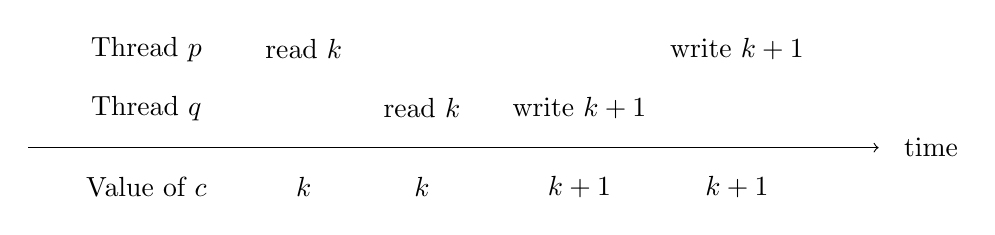
\begin{tikzpicture}
\node at (-1,0.75) {Thread $p$};
\node at (-1,0) {Thread $q$};
\node at (-1,-1){Value of $c$};

\node at (1,0.75) {read $k$};
\node at (1,-1) {$k$};

\node at (2.5,0.0) {read $k$};
\node at (2.5,-1) {$k$};

\node at (4.5,0) {write $k+1$};
\node at (4.5,-1) {$k+1$};

\node at (6.5,0.75) {write $k+1$};
\node at (6.5,-1) {$k+1$};

\draw[->] (-2.5, -0.5) -- (8.3, -0.5);

\node at (8.5, -0.5) [anchor=west]{time};
\end{tikzpicture}
\end{myimage}
\caption {Competition for access to a shared resource.}
\label{fig/competition}
\end{myfigure}
%
Assume the scenario described in figure~\ref {fig/competition}.
Thread $p$ reads the value of counter $c$, then gives control to $q$.
In its turn, $q$ reads the value of $c$, then writes the value $k+1$
to $c$.  The thread $p$ resumes control and writes the value $k+1$ to
$c$. The final value of $c$ is therefore $k+1$ instead of $k+2$.

This classic problem can be resolved by using locks that
prevent arbitrary interleaving of $p$ and $q$.

Locks are shared objects that can be held by at most a single thread
within a program at a time. A lock is created by the function
\pthreadcall[mutex]{create}.
%
\begin{codefile}{tmpmutex.mli}
  type t
\end{codefile}
%
\begin{listingcodefile}{tmpmutex.mli}
val $\libvalue{Mutex}{create}$ : unit -> t
\end{listingcodefile}
%
This operation a constructs a new lock, initially not held by any thread.
To acquire an existing lock, it is necessary to call the function
\pthreadcall[mutex]{lock} with the lock as argument. If the lock is
held by another thread, the caller is frozen until the lock is released.
A lock must be released explicitly by the thread that holds it, by
calling \pthreadcall[mutex]{unlock}.
%
\begin{listingcodefile}{tmpmutex.mli}
val $\libvalue{Mutex}{lock}$ : t -> unit
val $\libvalue{Mutex}{unlock}$ : t -> unit
\end{listingcodefile}
%
The \ml+lock+ call behaves like \ml+Thread.join+ with respect to
signals: if the thread receives a signal while executing \ml+lock+,
the signal will be noted ({\ie} the {\ocaml} runtime will be notified
that the signal has arrived), but the thread will continue to wait so
that \ml+lock+ effectively returns only when the lock has been
acquired, and never raises the \ml+EINTR+ exception.  The real
treatment of the signal by {\ocaml} will happen only upon the return
from \ml+lock+.

We can also try to acquire a lock without blocking by calling
\pthreadcall[mutex]{trylock}
%
\begin{listingcodefile}{tmpmutex.mli}
val $\libvalue{Mutex}{try\_lock}$ : t -> bool
\end{listingcodefile}
%
This function returns \ml+true+ if the lock has been acquired and
\ml+false+ otherwise.  In the latter case, execution is not suspended
since the lock is not acquired. The thread can therefore do something
else and eventually return and try its luck later.

\begin{example}

Incrementing a global counter used by several threads poses a
synchronization problem: the instants between reading the value of the
counter and writing the incremented value are in a critical region,
{\ie} two threads cannot be in this region at the same time. The
synchronization can easily be managed with a lock.
%
\begin{listingcodefile}{cthread.ml}
type counter = { lock : Mutex.t; mutable counter : int }
let newcounter() = { lock = Mutex.create(); counter = 0 }
let addtocounter c k = 
  Mutex.lock c.lock; 
  c.counter <- c.counter + k; 
  Mutex.unlock c.lock;;
\end{listingcodefile}
%
The sole read operation on the counter poses no problem. It can be
performed in parallel with a modification of the counter: the result
will simply be the value of the counter just before or just after the
modification, both results being consistent.
\end{example}

A common pattern is to hold a lock temporarily during a function call.
It is of course necessary to make sure to release the lock at the end
of the call, whether the call succeeded or failed. We can abstract
this behavior in a library function:
\begin{codefile}{misc.mli}
val run_with_lock : Mutex.t -> ('a -> 'b) -> 'a -> 'b
\end{codefile}
\begin{listingcodefile}{misc.ml}
let run_with_lock l f x = 
  Mutex.lock l; try_finalize f x Mutex.unlock l
\end{listingcodefile}
In the preceding example, we could also have written:
\begin{codefile}{cthread.ml}
open Misc;;
\end{codefile}
\begin{listingcodefile}{cthread.ml}
let addtocounter c =
  Misc.run_with_lock c.lock (fun k -> c.counter <- c.counter + k)
\end{listingcodefile}

\begin{example}
An alternative to the model of the server with threads is to start a
number of threads in advance which handle requests in parallel.
%
\begin{codefile}{farm.mli}
open Unix
\end{codefile}
%
\begin{listingcodefile}{farm.mli}
val tcp_farm_server : 
  int -> (file_descr -> file_descr * sockaddr -> 'a) -> sockaddr -> unit
\end{listingcodefile}
%
The \ml+tcp_farm_server+ function behaves like \ml+tcp_server+ but
takes an additional argument which is the number of threads to start,
each of which will become a server at the same address. The advantage
of a pool of threads is to reduce the time to handle each connection
by eliminating the cost of creating a thread for it, since they are
created once and for all.
%
\begin{codefile}{farm.ml}
open Sys;;
open Unix;;
\end{codefile}
%
\begin{listingcodefile}{farm.ml}
let tcp_farm_server n treat_connection addr = 
  let server_sock = Misc.install_tcp_server_socket addr in 
  let mutex = Mutex.create() in
  let rec serve () =
    let client = 
      Misc.run_with_lock mutex 
        (Misc.restart_on_EINTR accept) server_sock in
    treat_connection server_sock client;
    serve () in
  for i = 1 to n-1 do ignore (Thread.create serve ()) done;
  serve ();;
\end{listingcodefile}
The only precaution to take is to ensure mutual exclusion around the
\ml+accept+ so that only one of the threads accepts a connection at a
time. The idea is that the \ml+treat_connection+ function performs a
sequential treatment, but it is not a requirement~---~we can
effectively combine a pool of threads with the creation of new
threads, which can be dynamically adjusted depending on the load.
\end{example}

Acquisition of a lock is an inexpensive operation when it succeeds
without blocking. It is generally implemented with a single
\quotes{test-and-set} instruction provided by all modern processors
(plus other small costs that are involved, such as updating caches).
However, when the lock is not available, the process must be suspended
and rescheduled later, which involves a significant additional cost.
We must therefore incur this penalty only for a real suspension of a
process in order to give control to another, and not for its potential
suspension during the acquisition of a lock.  Consequently, we will
almost always want to release a lock as soon as possible and take it
back later if necessary, rather than simply holding onto the lock.
Avoiding these two operations would have the effect of enlarging the
critical region and therefore the frequency with which another thread
finds itself effectively in competition for the lock and in need of
suspension.

Locks reduce interleaving.  In return, they increase the risk of
deadlock.  For example, there is a deadlock if a thread $p$ waits for
a lock $v$ held by a thread $q$ which itself waits for a lock $u$ held
by $p$.  (In the worst case, a thread waits for a lock that it holds
itself.)  Concurrent programming is difficult, and guarding against
deadlock is not always easy.  A simple way of avoiding this situation
that is often possible consists of defining a hierarchy among the
locks and ensuring that the order in which the locks are acquired
dynamically respects the hierarchy: a thread never acquires a lock
unless that lock is dominated by all the other locks that the thread
already holds.

\section{Complete example: {\http} relay}
\label{ex/th-relais}

We will modify the {\http} relay developed in the preceding chapter
so that it services requests using threads.

Intuitively, it suffices to replace the \ml+establish_server+ function
that creates a process clone with a function that creates a
thread.  We must however take certain precautions.  The challenge
with threads is that they share the entire memory space.  We must
therefore ensure that the threads are not \quotes{stepping on each
other's toes} with one undoing what was just done by another.
That typically happens when two threads modify the same mutable
structure in parallel.

In the case of the {\http} server, there are several changes to make.
Let us start by resolving problems with access to resources.  The
\ml+proxy_service+ function, described in section~\ref{page/get_url},
handles the treatment of connections.  Via the intermediary functions
\ml+parse_host+, \ml+parse_url+ and \ml+parse_request+, it calls the
\ml+regexp_match+ function which uses the \ml+Str+ library.  However,
this library is not re-entrant (the result of the last search is
stored in a global variable). This example shows that we must beware
of calls to innocent-looking functions that hide potential collisions.
In this case we will not rewrite the \ml+Str+ library but simply
sequentialize its use.  It suffices to protect calls to this library
with locks (and there is really no other choice). We must still take
the precaution of releasing the lock when returning from the function
abnormally due to an exception.

To modify the existing code as little as possible, we can just rename
the definition of \ml+regexp_match+ in the \ml+Url+ module as
\ml+unsafe_regexp_match+ and then define \ml+regexp_match+ as a
protected version of \ml+unsafe_regexp_match+.
%
\begin{codefile}{thurl.ed}
f th/url.ml
r url.ml
/^let regexp_match/s/regexp_match/unsafe_regexp_match/
/^let/-1a
open Misc;;
\end{codefile}
%
\begin{listingcodefile}{thurl.ed}
let strlock = Mutex.create();;
let regexp_match r string =
  Misc.run_with_lock strlock (unsafe_regexp_match r) string;;
\end{listingcodefile}

The change is rather minimal.  It should be noted that the
\ml+regexp_match+ function includes both the expression matching and
the extraction of the matched groups.  It would definitely have been
incorrect to protect the \ml+Str.string_match+ and
\ml+Str.matched_group+ functions individually.

Another solution would be to rewrite the analysis functions without using
the \ml+Str+ library.  But there is no reason for such a choice, since
synchronizing the library primitives is easy to do and does not turn
out to be a source of inefficiency.  Obviously, a better solution
would be for the \ml+Str+ library to be re-entrant in the first place.

The other functions that are called are already re-entrant, in particular
the \ml+Misc.retransmit+ function that allocates different buffers for
each call.

However, there are still some precautions to take regarding error
handling.  The handling of a connection by a thread must be robust, as
explained above. In particular, in case of error, the other threads
must not be affected. In other words, the thread must terminate
\quotes{normally}, properly closing the connection in question and
going back to accepting other pending connections.  We must first of
all replace the call to \ml+exit+ in \ml+handle_error+ because it is
essential not to kill the whole process.  A call to \ml+Thread.exit+
would not be correct either, because thread termination does not close
its (shared) descriptors, the way the system does for process
termination.  An error in the handling of a connection would leave the
connection open.  The solution consists of raising an \ml+Exit+
exception that allows the finalization code to do what is required.
We must now protect \ml+treat_connection+ by catching all errors, in
particular \ml+Exit+ but also \ml+EPIPE+, which can be raised if the
client closes the connection prematurely.  We will take care of this
by using a protected function.
%
\begin{codefile}{thurl.ed}
.
1;#
/handle_error/;#
-1a
exception Exit;;
.
.,++s/exit 2/raise Exit/
wq
\end{codefile}
%
\begin{codefile}{thproxy.ed}
f th/proxy.ml
r proxy.ml
/let proxy/-1a
\end{codefile}
\begin{listingcodefile}{thproxy.ed}
let allow_connection_errors f s = 
  try f s with Exit | Unix_error(EPIPE,_,_) -> ()
\end{listingcodefile}
%
\begin{codefile}{thproxy.ed}
.
/let treat_connection/c
\end{codefile}
%
\begin{listingcodefile}{thproxy.ed}
let treat_connection s = 
  Misc.co_treatment s (allow_connection_errors proxy_service) in
\end{listingcodefile}
%
\begin{codefile}{thproxy.ed}
.
wq
\end{codefile}

\begin{exercise}[noanswer]
Rewrite the proxy for the {\http}/1.1 protocol using threads.
\end{exercise}

\begin{exercise}[noanswer]
Coroutines can be seen as a very particular kind of threads where each
process must surrender control explicitly before another can execute.
Give an implementation of coroutines using threads.
\end{exercise}

\section{Conditions}

The functions described in this section are defined in the
\libmodule{Condition} module.

Synchronization with locks is very simple, but it is not sufficient:
locks allow waiting for shared data to be free, but do not allow
waiting for the data to have a particular state.  Let us replace the
example of a counter by a (first-in/first-out) queue shared among
several threads.  Adding a value to the queue can be synchronized by
using a lock as above, since no matter what the state of the queue,
we can always add an element.  But what about removing an element
from the queue?  What should be done when the queue is empty?  We
cannot hold the lock while waiting for the queue to be filled, because
that would completely prevent another thread from filling the queue.
So it must be released.  But how can we know when the queue is no
longer empty, except by testing it periodically?  This solution,
called \quotes{busy-waiting}, is definitely not satisfactory.  Either
it consumes computing cycles unnecessarily (period too short) or else
it it is not reactive enough (period too long).

\emph{Conditions} provide a solution to this problem.  A thread that
holds a lock can wait for a condition object until another thread
sends a signal on that condition.  As with locks, conditions are
passive structures that can be manipulated by synchronization
functions.  They can be created by the \pthreadcall[cond]{create}
function.
%
\begin{codefile}{tmpcondition.mli}
type t
\end{codefile}
%
\begin{listingcodefile}{tmpcondition.mli}
val $\libvalue{Condition}{create}$ : unit -> t
\end{listingcodefile}
%
A process $p$ that \emph{already holds} a lock \ml+v+ can wait on a
condition \ml+c+ and the \ml+v+ by calling \pthreadcall[cond]{wait}.
The process $p$ informs the system that it is waiting on the condition
\ml+c+ and the lock \ml+v+, then releases the lock \ml+v+ and goes to
sleep.  It will not be woken up by the system until another thread $q$
signals a change on the condition \ml+c+ and the lock \ml+v+ is
available; the process $p$ will then hold the lock \ml+v+ again.
%
\begin{listingcodefile}{tmpcondition.mli}
val $\libvalue{Condition}{wait}$ : t -> Mutex.t -> unit
\end{listingcodefile}
%
Note: it is an error to call \ml+wait c v+ without holding the lock
\ml+v+.  The behavior of \ml+wait c v+ with respect to signals is the
same as for \ml+Mutex.lock+.

When a thread signals a change on a condition, it can either ask for
all threads waiting on that condition to be woken up
(\pthreadcall[cond]{broadcast}), or else for just one of them to be
woken up (\pthreadcall[cond]{signal}).
%
\begin{listingcodefile}{tmpcondition.mli}
val $\libvalue{Condition}{signal}$ : t -> unit
val $\libvalue{Condition}{broadcast}$ : t -> unit
\end{listingcodefile}
%
Sending a signal or a broadcast on a condition does not require
holding a lock (unlike waiting), in the sense that it will not trigger
a \quotes{system} error.
%%
%% Est-ce vrai? c'est � celui qui se met en attente � avoir pris le verrou
%% avant de tester, puis fait wait. Il est donc s�r que la condition n'est
%% pas vrai � ce moment l�. 
%% 
However, it can sometimes be a programming error.
%% En effet, �mettre un signal sans poss�der le verrou sur
%% lequel les r�cepteurs de ce signal sont en attente signifie que
%% l'�mission du signal n'est pas synchronis�e avec la mise en attente et
%% peut donc se produire avant la mise en attente qu'il est suppos�
%% interrompre: le signal sera alors ignor� et l'attente jamais
%% interrompue (voir l'exemple des queues ci-dessous).  

The choice between waking up one thread or all the threads depends on
the problem.  To consider the example of the queue again, if a thread
adds an element to an empty queue, there is no need to wake up all the
others, since only one will effectively be able to remove that
element.  On the other hand, if it adds a number of elements that is
either not statically known or very large, it must wake up all the
threads.  Note that if adding an element to a non-empty queue does not
send a signal, then adding an element to an empty queue must send a
broadcast, since it could be followed immediately by another addition
(without a signal) and therefore behave like a multiple addition.
In summary, either send a signal on every addition, or send a
broadcast only when adding to an empty queue.
The choice between these two strategies is a bet on whether the queue
is usually empty (first solution) or usually non-empty (second
solution).

Often, one thread knows only an approximation of the reason why
another thread is waiting on a condition.  It will therefore signal
the condition whenever the situation \emph{might} be what the other
thread is waiting for.  An awakened thread, therefore, cannot assume
that the condition it was waiting is now satisfied.  It must, in
general, re-test the state of its shared data, and if necessary wait
on the condition again.  This does not consitute busy-waiting, because
it only happens when another thread signals the condition.

Here is another justification for this approach: when a thread has
just produced a lot of some resource and wakes all the others using a
\ml+broadcast+, nothing prevents the first one that wakes up from
being greedy and exhausting the entire resource.  The second one to
wake up must go back to sleep, hoping to be luckier next time.

We can now give a concrete solution for shared queues.  The \ml+queue+
structure defined in the \ml+Queue+ module is extended with a lock and
a \ml+non_empty+ condition.
%
\begin{listingcodefile}[style=numbers]{thcheck.ml}
type 'a t = 
  { queue : 'a Queue.t; lock : Mutex.t; non_empty : Condition.t }
let create () = 
  { queue = Queue.create(); 
    lock = Mutex.create(); non_empty = Condition.create() }

let add e q = 
  Mutex.lock q.lock; 
  if Queue.length q.queue = 0 then Condition.broadcast q.non_empty;$\label{prog:broadcast}$
  Queue.add e q.queue; 
  Mutex.unlock q.lock;;

let take q = 
  Mutex.lock q.lock; 
  while Queue.length q.queue = 0 $\label{prog:lock}$
  do Condition.wait q.non_empty q.lock done;  $\label{prog:slock}$
  let x = Queue.take q.queue in
  Mutex.unlock q.lock; x;;
\end{listingcodefile}
%
Addition never blocks, but we must not forget to signal
the \ml+non_empty+ condition when the list is empty beforehand,
because it is possible that someone is waiting on the condition.

Removal is a little more complicated: after acquiring the lock, we
must try to remove an element from the queue. If the queue is empty,
we must wait on the \ml+non_empty+ condition.  When awakened, we try
again, knowing that we already have the lock.

As explained above, the \ml+broadcast q.non_empty+ signal
(line~\ref{prog:broadcast}) is executed by a thread $p$ already in
possession of the lock \ml+q.lock+.
This implies that a reader thread $q$ executing the \ml+take+ function
cannot be between line~\ref{prog:lock} and~\ref{prog:slock}
where it would have verified that the queue is empty but not yet have
gone to sleep.  In this case, the signal sent by $p$ would be
ineffective and ignored, since $q$ has not gone to sleep yet; but $q$
would then go to sleep and not be woken up, because $p$ has already
sent its signal.
The lock therefore guarantees that either $q$ is already asleep or
else has not yet tested the state of the queue.

\begin{exercise}
Implement a variant in which the queue is bounded: addition to the
queue becomes blocking when the size of the queue reaches a fixed
value. (In a concurrent world, we might need this scheme to avoid
having a producer that produces endlessly while the consumer is
blocked.)
\end{exercise}
\begin{answer}
We must introduce an additional \ml+non_full+ condition.
We also add a \ml+size+ field to allow queues of different sizes.
%
\begin{listingcodefile}{thtqueue.ml}
type 'a t = 
    { queue : 'a Queue.t; size : int; lock : Mutex.t;
      non_empty : Condition.t; non_full : Condition.t; }
      
let create k = 
  if  k > 0 then
    { queue = Queue. create(); size = k; lock = Mutex. create(); 
      non_empty = Condition. create(); non_full = Condition.create() }
  else failwith "Tqueue.create: empty size";;
\end{listingcodefile}
%
Addition is a combination of the preceding versions of the
\ml+add+ and \ml+take+ functions above.
%
\begin{listingcodefile}{thtqueue.ml}
let add x q = 
  Mutex.lock q.lock;
  while Queue.length q.queue = q.size 
  do Condition.wait q.non_full q.lock done;
  if Queue.is_empty q.queue then Condition.broadcast q.non_empty;
  Queue.add q x;
  Mutex.unlock q.lock;;
\end{listingcodefile}
%
Removal is symmetric to addition (and must now signal \ml+non_full+
when the queue is full beforehand), and is left to the reader.
%
\begin{codefile}{thtqueue.ml}
let take q = 
  Mutex.lock q.lock;
  while Queue.length q.queue = 0 
  do Condition.wait q.non_empty q.lock done;
  if Queue.length q.queue = q.size then Condition.broadcast q.non_full;
  let x = Queue.take q.queue in
  Mutex.unlock q.lock; x;;
\end{codefile}
%
We get the behavior of unbounded queues by choosing \ml+max_int+ for
\ml+size+.
\end{answer}



\section{Event-based synchronous communication}

The functions described in this section are defined in the
\libmodule{Event} module.

Locks and conditions together allow all forms of synchronization to be
expressed.  However, their implementation is not always easy, as shown
by the example of the initially simple queue whose synchronization
code subsequently turned out to be subtle.

Event-based synchronous communication is a collection of higher-level
communication primitives that tend to facilitate concurrent
programming.  The primitives in the \ml+Event+ module were initially
developed by John Reppy as an extension of the \emph{Standard ML}
language called \emph{Concurrent ML}~\cite{CML}.  In {\ocaml}, these
primitives are located above the more elementary synchronization of
locks and conditions.

Communication occurs by sending \emph{events} along \emph{channels}.
Channels are like \quotes{lightweight pipes}: they allow communication
among threads in the same program and take care of synchronization
between producers and consumers.  A channel carrying values of type
\ml+'a+ has the type \ml+'a Event.channel+.  Channels are homogeneous
and therefore always carry values of the same type.  A channel is
created with the \ml+new_channel+ primitive.
%
\begin{codefile}{tmpevent.mli}
type 'a channel
type +'a event
\end{codefile}
%
\begin{listingcodefile}{tmpevent.mli}
val $\indexlibvalue{Event}{new\_channel}$ : unit -> 'a channel
\end{listingcodefile}
%
Sending or receiving a message is not done directly, but through the
intermediary of an event.  An elementary event is \quotes{sending a
message} or \quotes{receiving a message}.  They are constructed by
means of the following primitives:
%
\begin{listingcodefile}{tmpevent.mli}
val $\indexlibvalue{Event}{send}$ : 'a channel -> 'a -> unit event
val $\indexlibvalue{Event}{receive}$ : 'a channel -> 'a event
\end{listingcodefile}
%
Construction of a message does not have an immediate effect: it just
creates a data structure describing the action to be done.  To make an
event happen, the thread must synchronize with another thread wishing
to make the complementary event happen.  The \ml+sync+ primitive
allows a thread to wait for the occurrence of the event passed
as argument.
%
\begin{listingcodefile}{tmpevent.mli}
val $\indexlibvalue{Event}{sync}$ : 'a event -> 'a
\end{listingcodefile}
%
Thus, to send a value \ml+v+ on the channel \ml+c+, one can execute
\ml+sync (send c v)+.  The thread is suspended until the event occurs,
that is to say until another thread is ready to receive a value on the
channel \ml+c+.  In a symmetric fashion, a thread can wait for a
message on channel \ml+c+ by performing \ml+sync (receive c)+.

There is a competition among all the producers on one hand and all the
consumers on the other.  For example, if several threads try to send a
message on a channel but only one is ready to read it, it is clear
that only one producer will make the event occur.  The others will
remain suspended, without even noticing that another was
\quotes{served} ahead of them.

The competition can also occur within the same thread.
Multiple events can be combined by the \ml+choose+ primitive.
%
\begin{listingcodefile}{tmpevent.mli}
val $\indexlibvalue{Event}{choose}$ : 'a event list -> 'a event
\end{listingcodefile}
%
The resulting event is an offer, in parallel, of the events passed as
arguments, and occurs when exactly one of them occurs.  We distinguish
between the offer of an event and its occurrence.  The call
\ml+sync (choose [e1; e2])+ synchronizes by offering a choice of two events
\ml+e1+ and \ml+e2+, but only one of the two events will effectively
occur (the offer of the other event will be simultaneously cancelled).
The \ml+wrap_abort+ primitive allows an event to handle being
cancelled.
%
\begin{listingcodefile}{tmpevent.mli}
val $\indexlibvalue{Event}{wrap\_abort}$ : 'a event -> (unit -> unit) -> 'a event
\end{listingcodefile}
%
The call \ml+wrap_abort e f+ creates an event that is equivalent to
\ml+e+, but if it is not chosen during synchronization, then the
function \ml+f+ is executed.  (This is only interesting when it is
part of a complex event.)

A thread can try to synchronize on an event without blocking (somewhat
like \ml+Mutex.try_lock+) with \ml+poll+.
%
\begin{listingcodefile}{tmpevent.mli}
val $\indexlibvalue{Event}{poll}$ : 'a event -> 'a option
\end{listingcodefile}
%
The call \ml+poll e+ offers the event \ml+e+ but if it cannot occur
immediately, it cancels the offer rather than blocking and has no
effect (or more exactly, behaves as if the expression \ml+poll e+ had
been replaced by the value \ml+None+).  By contrast, if the event can
happen immediately, then it behaves as if the thread had done
\ml+sync e+, except that the value \ml+Some v+ is returned
rather than \ml+v+.

\begin{example}
In example~\ref {ex/crible-copro} of the Sieve of Eratosthenes,
the communication between different threads is done with pipes as in
the original program, using system memory (the pipe) as intermediary.
One might think that it would be more efficient to communicate
directly by using the memory of the process.  A simple solution
consists of replacing the pipe by a channel on which integers are sent.

Sending integers on the channel is not sufficient, because we must
also be able to detect the end of the stream.  The simplest is
therefore to pass elements of the form \ml+Some n+ and to terminate by
sending the value \ml+None+.  To minimize the changes, we will go back
to the code in example~\ref{ex/crible}.  We simulate pipes and the
functions for reading and writing pipes by channels and functions for
reading and writing channels.

It is sufficient to take the previous version of the program and
change the input/output functions to ones that read and write a channel,
rather than an input/output buffer from the \ml+Pervasives+ library.
For example, we can insert the following code at line~2:
%
\begin{codefile}{theventcrible.ed}
f th/eventcrible.ml
r th/crible.ml
/let input_int/d
/let output_int/d
/generate/-1a
\end{codefile}
%
\begin{listingcodefile}{theventcrible.ed}
let pipe () = let c = Event.new_channel() in c, c
let out_channel_of_descr x = x
let in_channel_of_descr x = x

let input_int chan = 
  match Event.sync (Event.receive chan) with
  | Some v -> v 
  | None -> raise End_of_file
let output_int chan x = Event.sync (Event.send chan (Some x))
let close_out chan = Event.sync (Event.send chan None);;
\end{listingcodefile}
%
\begin{codefile}{theventcrible.ed}
.
wq
\end{codefile}

However, if we compare the efficiency of this version with the
previous one, we find that it is twice as slow.  Communication of each
integer requires a synchronization between two threads and therefore
several system calls for acquiring and releasing locks.  On the other
hand, communication via pipes uses buffered \io{} that allows several
thousand integers to be exahanged with each system call.

To be fair, one should also provide buffered communication on
channels, using the channel only to exchange a packet of integers.
The child can accumulate the results in a private queue, to which it
can therefore write without synchronization.  When the queue is full,
or upon an explicit request, it is emptied by synchronizing on the
channel.  The parent has its own queue that it receives by
synchronizing and empties gradually.

Here is a solution:
%
\begin{codefile}{thbuffercrible.ed}
f th/buffercrible.ml
r th/crible.ml
/generate/-1a
\end{codefile}
%
\begin{listingcodefile}{thbuffercrible.ed}
type 'a buffered = 
    { c : 'a Queue.t Event.channel; 
      mutable q : 'a Queue.t; 
      size : int }

let pipe () = let c = Event.new_channel() in c, c;;

let size = 1024;;
let out_channel_of_descr chan = 
  { c = chan; q = Queue.create(); size = size };;
let in_channel_of_descr = out_channel_of_descr;;

let input_int chan = 
  if Queue.length chan.q = 0 then begin
    let q = Event.sync (Event.receive chan.c) in
    if Queue.length q > 0 then chan.q <- q
    else raise End_of_file
  end;
  Queue.take chan.q;;

let flush_out chan = 
  if Queue.length chan.q > 0 then Event.sync (Event.send chan.c chan.q);
  chan.q <- Queue.create();;

let output_int chan x = 
  if Queue.length chan.q = size then flush_out chan;
  Queue.add x chan.q

let close_out chan = 
  flush_out chan;
  Event.sync (Event.send chan.c chan.q);;
\end{listingcodefile}
%
\begin{codefile}{thbuffercrible.ed}
.
wq
\end{codefile}
%
This version allows us to regain efficiency comparable to (but not
better than) the version with pipes.

Compared to the original version with processes and pipes, there are
two potential advantages. First, threads are more lightweight and less
costly to launch.  Second, communication on a channel merely passes a
pointer, without copying.  But these advantages are not noticeable
here, because the number of threads created and the data exchanged are
not big enough compared to the cost of system calls and compute time.

In conclusion, we can say that communication between threads has a
cost of up to one system call (if the process must be suspended) and
the cost can be significantly reduced by buffering communication and
sending larger structures less often.
\end{example}

\begin{exercise}[noanswer]
An {\http} server can be subjected to a high, bursty load.  To improve
response time, we can refine the architecture of an {\http} server by
always keeping a dozen threads ready to handle new requests. This means
that a thread does not handle only a single request, but a potentially
infinite series of requests that it reads from a queue.

To avoid overloading the machine, we can limit the number of threads
to a reasonable value beyond which the overhead of managing tasks
exceeds the latency for servicing requests (time spent waiting for
data on disk, \etc).  After that, we can keep some connections waiting
to be handled, and then finally we can refuse connections.  When the
load diminishes and the number of threads is above the \quotes{ideal}
value, some of them are allowed to die and the others remain ready for
the next requests.

Transform example~\ref{ex/th-relais} into this architecture.
\end{exercise}


\section{Implementation details}

\paragraph {Implementation of threads in Unix}

The Unix system was not originally designed to provide support for
threads.  However, most modern Unix implementations now offer such
support.  Nevertheless, threads remain an add-on that is sometimes
apparent.  For example, when using threads it is strongly discouraged
to use \ml+fork+ except when doing \ml+exec+ immediately afterward.
In effect, \ml+fork+ copies the current thread, which becomes a
crippled process that runs believing it has threads when in fact they
do not exist.  The parent continues to run normally as before.
The special case of a call to \ml+fork+ where the child immediately
launches another program does not cause the parent any problem.
Luckily, since that is the only way to start other programs!

Inversely, one can do \ml+fork+ (not followed by \ml+exec+), and then launch
several threads in the child and the parent, without any problem.

\paragraph {Native and simulated implementation in OCaml}
\label{sec/thread-implementation}

When the underlying operating system has threads, {\ocaml} can provide
a native implementation of threads, leaving their management to the
operating system as much as possible.  Each thread then lives in a
different Unix process but shares the same address space.

When the system does not provide support for threads, {\ocaml} can
emulate them.  All the threads then execute in the same Unix process,
and their management, including their scheduling, is handled by the
{\ocaml} runtime system.  However, this implementation is only
available when compiling to bytecode.

The {\ocaml} system provides the same programming interface for the
native and simulated versions of threads. The implementation of
threads is therefore split: one implementation for the emulated
version that includes its own task controller, and another
implementation that is based on \textsc{posix}~(1003.1c) threads and
lifts the corresponding library functions to the level of the {\ocaml}
language.  In the process, the {\ocaml} language handles certain
simple administrative tasks and ensures an interface identical to the
emulated version.  This guarantees that a program compilable on one
Unix architecture remains compilable on another Unix architecture.
However, whether threads are emulated or native can change the
synchronization of calls to the C library, and therefore change,
despite everything, the semantics of the program.  It is therefore
necessary to take certain precautions before believing that a program
will behave the same way in these two versions.  In this chapter, the
discussion will mainly concern these two implementations, but recall
that by default, we have taken the viewpoint of a native
implementation.

To use emulated threads, one must pass the \ml+-vmthreads+ option
instead of \ml+-threads+ to the \ml+ocamlc+ compiler. This option is
not accepted by the \ml+ocamlopt+ compiler.

\paragraph{Sequentialization of {\ocaml} code}

The implementation of threads in {\ocaml} must face one of the
peculiarities of the {\ocaml} language: the automatic management of
memory and its high consumption of allocated data.  The solution
adopted, which is the simplest and also generally the most efficient,
is to sequentialize the execution of {\ocaml} code in all threads: a
lock in the runtime system prevents two threads from executing
{\ocaml} code simultaneously.  This seems contrary to the whole idea
of threads, but it is not, since the lock is released before blocking
system calls and reacquired upon return.  Other threads can therefore
take control at that moment.  A special case of such a system call is
the call to \ml+sched_yield+, performed at regular intervals to
suspend the running thread and give control to another.

On a multiprocessor machine, the only source of true parallelism comes
from the execution of C code and system calls.  On a uniprocessor
machine, the fact that the {\ocaml} code is sequentialized is not
really noticeable.

The programmer cannot rely on this sequentialization, because one
thread can give control to another at almost any moment.  With one
exception, the sequentialization guarantees memory coherence: two
threads always have the same view of memory, except perhaps when they
execute C code.  In effect, the passing of the lock implies a
synchronization of the memory: a read operation by one thread
occurring after a write operation to the same address by another
thread will always return the freshly-written value, with no need for
additional synchronization.

\paragraph {Threads and signals}

Generally speaking, using signals is already delicate with a single
thread due to their asynchronous character.  It is even more so in the
presence of multiple threads because of the addition of new
difficulties: which thread should a signal be sent to?  To all, to the
primary one, or to the one currently running?  What happens if one
thread sends a signal to another?  In fact, threads were implemented
before answering these questions, and different implementations can
behave differently with respect to signals.

The \ml+Thread.join+, \ml+Mutex.lock+, and \ml+Condition.wait+,
despite being long system calls, are not interruptible by a signal.
(They cannot therefore fail with the \ml+EINTR+ error.)  If a signal
is sent while waiting, it will be received and handled when the call
returns.

The \textsc{posix} standard specifies that the signal handler is
shared among all the threads and in contrast the signal mask is
private to each thread and inherited upon creation of a thread.  But
the behavior of threads with respect to signals remains largely
underspecified and therefore non-portable.

It is therefore preferable to avoid as much as possible the use of
asynchronous signals (such as \ml+sigalrm+, \ml+sigvtalrm+,
\ml+sigchld+, \etc) with threads. These can be blocked and examined
with \ml+Thread.wait_signal+.  One can dedicate a thread to signal
handling and nothing else: it can wait for the reception of signals,
undertake the necessary actions, and update certain information
examined by other threads.

In addition, {\ocaml} threads (since version 3.08) use the
\ml+sigvtalarm+ signal internally to implement preemption of threads.
This signal is therefore reserved and must not be used by the program
itself, since there is a risk of interference.

\begin{codefile}{thmisc.ed}
f th/misc.mli
r misc.mli
$r th/misc.MLI
w
f th/misc.ml
1,$ d
r misc.ml
$r th/misc.ML
wq
\end{codefile}







%------------------------------------------------------------------------------
% Copyright (c) 1991-2014, Xavier Leroy and Didier Remy.  
%
% All rights reserved. Distributed under a creative commons
% attribution-non-commercial-share alike 2.0 France license.
% http://creativecommons.org/licenses/by-nc-sa/2.0/fr/
%
% Translation by
%------------------------------------------------------------------------------

\chapter*{\label{sec/more}\ifhtml{\aname{htocmore}}Going further}
\addcontentsline{toc}{chapter}{\ifhtml{\ahrefloc{htocmore}}{Going further}}
\cutname{more.html}

We have shown how \ocaml's \libmodule{Sys}, \libmodule{Unix}, and
\libmodule{Threads} modules can be used to program applications that
interact with the operating system.

These modules allow the invocation of the most important Unix system calls
directly from {\ocaml}. Some of these calls were replaced by higher-level
functions, either to facilitate programming or to maintain invariants
needed by {\ocaml}'s runtime system. In any case, this higher-level
access to the Unix system streamlines the development of applications.

Not every feature of the Unix system is available through these
modules, however it is still possible to access the missing ones by
writing C bindings.

Another useful library is Cash~\cite{Cash} which focuses on writing
scripts directly in {\ocaml}. This library completes the \ml+Unix+
module in two different ways. First, in addition to a few helper
functions to write scripts, it provides, on top of the \ml+Unix+
module, a few system call variations to assist the programmer in
process and pipe management. Second, it offers additional entry points
to the Unix system.


\backmatter

%% Exercise answers
\ifnothtml{\chapter{Exercise answers}\inputexerciseanswers}

%% References
%------------------------------------------------------------------------------
% Copyright (c) 1991-2014, Xavier Leroy and Didier Remy.  
%
% All rights reserved. Distributed under a creative commons
% attribution-non-commercial-share alike 2.0 France license.
% http://creativecommons.org/licenses/by-nc-sa/2.0/fr/
%
% Translation by Daniel C. Buenzli
%------------------------------------------------------------------------------

\renewcommand{\bibname}{References}
\ifhtml{\renewcommand{\refname}{\aname{htocrefs}References}}
\begin{thebibliography}{9}
\cutname{references.html}
\ifhtml{\addcontentsline{toc}{chapter}{\ahrefloc{htocrefs}{References}}}

\bibcomment{OCaml}

\bibitem{Caml-Light}
Xavier Leroy, Michel Mauny. \emph{The Caml Light system, release 0.5.
Documentation and user's manual.} L-5 software, distributed by \textsc{inria}.

\bibitem{OCaml}
Xavier Leroy, Didier Rémy, Jacques Garrigue, Jérôme Vouillon and
Damien Doligez.
\emph{The {OCaml} system,
documentation and user's manual -- release 3.06.}
Documentation distributed by \textsc{inria} with the OCaml
system, August 2002.
\url{http://caml.inria.fr/pub/docs/manual-ocaml/}.

\bibitem{Cash}
Bruno Verlyck.
\emph{Cash, the Caml Shell -- release 0.20}.
Documentation distributed by \textsc{inria} with the Cash system, 2002. 
\url{http://pauillac.inria.fr/cash/}.

\bibcomment{Unix system programming}

\bibitem{man}
The Unix \texttt{man}ual, sections 2~and~3.

\bibitem{KP}
Brian Kernighan, Rob Pike. \emph{The Unix programming
environment}, Addison-Wesley.

\bibitem{R1} 
Jean-Marie Rifflet. \emph{La programmation sous Unix}. McGraw-Hill.

\bibitem{R2}
Jean-Marie Rifflet. \emph{La communication sous Unix}. McGraw-Hill.

\bibcomment{Unix kernel architecture}

\bibitem{BSD}
Samuel Leffler, Marshall McKusick, Michael Karels, John Quarterman.
\emph{The design and implementation of the 4.3 \textsc{bsd}
 Unix operating system},
Addison-Wesley.

\bibitem{Bach}
Maurice Bach. \emph{The design and implementation of the Unix operating
system}, Prentice-Hall.

\bibitem{Stevens/advanced}
Richard~W. Stevens.
\newblock \emph{Advanced Programming in the Unix Environment}.
\newblock Addison-Wesley, 1992.

\bibitem{Kay-Stevens/Practical}
Kay~A. Robbins and Steven Robbins.
\newblock \emph{Practical Unix Programming.
A Guide to Concurrency, Communication, and Multithreading}.
\newblock Prentice Hall, 1996.

\bibcomment{General knowledge on operating systems}

\bibitem{T3}
Andrew Tanenbaum. \emph{Modern Operating Systems},
Second Edition, Prentice-Hall, 2001. 
 

\bibitem{T1}
Andrew Tanenbaum. \emph{Operating systems, design and implementation},
Prentice-Hall.

\bibitem{T2}
Andrew Tanenbaum. \emph{Computer Networks}, Prentice-Hall.

\bibcomment{Typed communication of structured objects}

\bibitem{Dynamiques}
Xavier Leroy, Michel Mauny. \emph{Dynamics in ML}. Actes de \textsc{fpca}~91,
\textsc{lncs}~523, Springer-Verlag.

\bibitem{CML}
John H. Reppy. \emph{Concurrent Programming in ML}.
Cambridge University Press, 1999.     

\bibcomment{Threads programming}

\bibitem{Butenhof/threads}
David R. Butenhof. 
\emph{{P}rogramming with {\textsc{posix}} {T}hreads}.
Addison-Wesley, 1997.

\bibcomment{Applications}

\bibitem{Unison}
Pierce et al.
\emph{Unison File Synchronizer. Version 2.9.1.
User Manual and Reference}. 
Free software available from  
\url{http://www.cis.upenn.edu/~bcpierce/unison/}. 
\end{thebibliography}


\appendix

%% Index
\renewcommand{\preindexhook} {
  \ifhtml{\aname{htocindex}{}} %% how can I put that in the title?
  \ifhtmlelse{Links}{Pages} in bold refer to the description of 
  a \textsc{posix} system call.
  \ifnothtml{\medskip}}

\printindex
\ifhtml{\addcontentsline{toc}{chapter}{\ahrefloc{htocindex}{Index}}}
\cutname{docindex.html}

%% Add a blank page
\pagestyle{empty}
\newpage
\mbox{}

%% Include standard implementation in .ml to check against our signatures. 
\begin{codefile}{tmpunix.ml}include Unix;;\end{codefile}
\begin{codefile}{tmpsys.ml}include Sys;;\end{codefile}
\begin{codefile}{tmppervasives.ml}include Pervasives;;\end{codefile}
\begin{codefile}{tmpevent.ml}include Event;;\end{codefile}
\begin{codefile}{tmpmutex.ml}include Mutex;;\end{codefile}
\begin{codefile}{tmpthread.ml}include Thread;;\end{codefile}
\begin{codefile}{tmpcondition.ml}include Condition;;\end{codefile}
\end{document}

